\documentclass[answers]{exam}

% AMS packages
\usepackage{amsmath}
\usepackage{amsthm}
\usepackage{amsfonts}
\usepackage{amssymb}

% Used so the PDF is hyperlinked for convenience, and chapter/section numbers are in the PDF bookmarks
\usepackage[bookmarksnumbered,hidelinks]{hyperref}

% Used in copmlex tabular/table
% Needed for a table in one of the solutions
\usepackage{multirow}

% Make the margins not so large
% Cannot use for now because the page number at the bottom goes off page
%\usepackage[margin=0.75in]{geometry}

% Used to indent whole paragraphs
\usepackage{changepage}

% Needed to be able to do arithmetic when setting counters
\usepackage{calc}

% Needed to make title pages without page numbers in exam class
\usepackage{titling}

% Needed for customization of section headers
\usepackage{titlesec}

% For diagrams (e.g. Venn diagrams in section 1.4)
\usepackage{tikz}

% TODO: Should we migrate \newcommand to this, which better enforces arguments and gives much better error messages for missing arguments
% Useful for more advanced macro arguments (e.g. boolean values)
\usepackage{xparse}

% For Creative Commons license icons
\usepackage[scale=1.5]{ccicons}


% Import all our custom macros
% Common sets
\def\nats{{\boldsymbol{N}}}
\def\ints{{\boldsymbol{Z}}}
\def\rats{{\boldsymbol{Q}}}
\def\prats{\rats^+}
\def\reals{{\boldsymbol{R}}}
\def\es{\varnothing}

% Common variables/symbols
\def\vphi{\varphi}
\def\a{\alpha}
\def\b{\beta}
\def\g{\gamma}
\def\d{\delta}
\def\e{\varepsilon}
\def\z{\zeta}
\def\k{\kappa}
\def\l{\lambda}
\def\n{\nu}
\def\r{\rho}
\def\s{\sigma}
\def\t{\tau}
\def\x{\xi}
\def\w{\omega}
\def\W{\Omega}
\def\al{\aleph}

% Logic
\def\bic{\leftrightarrow}
\newcommand{\propP}[1]{\prop{P}(#1)}
\def\lxor{\veebar}

% For set-buider notation
\def\where{\mid}

% Other stuff
\def\dom{\mathrm{dom}\,}
\def\ran{\mathrm{ran}\,}

% Cardinality shortcuts
\def\cnats{{\al_0}}
\def\ccont{{2^\cnats}}

% Equivalence classes
\newcommand\eclass[2]{\squares{#1}_{#2}}

% Shortcuts that make writing easier
\newcommand\parens[1]{\left( #1 \right)}
\newcommand\squares[1]{\left[ #1 \right]}
\newcommand\braces[1]{\left\{ #1 \right\}}
\newcommand\angles[1]{\left\langle #1 \right\rangle}
\newcommand\ceil[1]{\left\lceil #1 \right\rceil}
\newcommand\floor[1]{\left\lfloor #1 \right\rfloor}
\newcommand\abs[1]{\left| #1 \right|}
\newcommand\dabs[1]{\left\| #1 \right\|}
\newcommand\vect[1]{\mathrm{\mathbf{#1}}}
\newcommand\conj[1]{\overline{#1}}
\newcommand\pset[1]{\mathcal{P}\left(#1\right)}
\newcommand\inv[1]{#1^{-1}}
\newcommand\prop[1]{\mathbf{#1}}
\def\rest{\restriction}
\newcommand\tet[2]{{^{#1}#2}}

% Families of set
\def\famF{\mathcal{F}}

% These are needed so that half-open intervals do not cause auto-indentation issues due to unmatched brackets
\newcommand\clop[1]{[#1)}
\newcommand\ilab[1]{#1)}

% Other miscellaneous stuff
\def\ss{\subseteq}
\def\pss{\subset}
\def\Seq{\mathrm{Seq}}
\def\prece{\preccurlyeq}
\def\sd{\bigtriangleup}

% Environment shortcuts
\newcommand\gath[1]{\begin{gather*} #1 \end{gather*}}
\newcommand\ali[1]{\begin{align*} #1 \end{align*}}
\newcommand\qproof[1]{\begin{proof} #1 \end{proof}}
\newcommand\bicproof[2]{
  $(\to)$ #1

  $(\leftarrow)$ #2
}
\newcommand\seteqproof[2]{
  $(\ss)$ #1

  $(\supseteq)$ #2
}

% Environment for indenting nested paragraphs (useful in case trees)
\newenvironment{indpar}
{
  \begin{adjustwidth}{1cm}{}
    }{
  \end{adjustwidth}
}

% Exercise, Theorem, and solution shortcuts
\newcommand\exercise[2]{{
      \renewcommand\label[1]{} % Needed to suppress multiply-defined label warning since the same question numbers are used in different sections
      \setcounter{subsubsection}{#1-1} % Subsubsections are used to that lemmas have the full nested numbering
      \stepcounter{subsubsection} % Need to increment this so that the lemma counter gets reset
      \setcounter{question}{#1-1} % Manually set the question number since we always know the exercise number
      \question{#2} % The actual exam class question
    }}
\newcommand\exerciseapp[3]{
  \setqf{#2}
  \exercise{#1}{#3}
  \setqf{}
}
\newcommand\theorem[2]{{
      \renewcommand\label[1]{} % Needed to suppress multiply-defined label warning since the same question numbers are used in different sections
      \setcounter{subsubsection}{#1-1} % Subsubsections are used to that lemmas have the full nested numbering
      \stepcounter{subsubsection} % Need to increment this so that the lemma counter gets reset
      \setcounter{question}{#1-1} % Manually set the question number since we always know the theorem number
      \question{#2} % The actual exam class question
    }}
\newcommand\theoremapp[3]{
  \setqf{#2}
  \theorem{#1}{#3}
  \setqf{}
}
\newcommand\sol[1]{
  \begin{solution}

    #1
  \end{solution}
}

% Main problem and theorem labels
\def\mainprob{\textbf{Main Problem.}}
\def\mainthrm{\textbf{Main Theorem.}}

% Saves some typing
\def\cbthrm{Cantor-Bernstein Theorem}

% Book title
\def\booktitle{
  Introduction to Set Theory \\
  Third Edition, Revised and Expanded \\
  by Karel Hrbacek and Thomas Jech
}


\title{
  \booktitle \\
  \ \\
  Solutions Manual \\
  \ \\
  \ \\
  by Dan Whitman
}

% So pages will break inside long equation environments
\allowdisplaybreaks

% Lemmas/Corollaries environments
\newtheorem{lem}{Lemma}[subsubsection]
\newtheorem{defin}[lem]{Definition}
\newtheorem{cor}[lem]{Corollary}
\newtheorem{thrm}[lem]{Theorem}

\begin{document}

% Setup section (chapter)  format
\titleformat{\section} % command
[hang] % shape
{\bfseries \Large} % format
{Chapter \thesection} % label
{12pt} % sep
{} % before-code
{} % after-code

% Setup subsection format
\titleformat{\subsection} % command
[hang] % shape
{\bfseries \large} % format
{\S \thesubsection} % label
{12pt} % sep
{} % before-code
{} % after-code

% Question label format
\newcommand\setqf[1]{\qformat{\hspace{0.5cm} \textbf{Exercise \thesubsection.\thequestion #1} \hfill \vrule depth 1em width 0pt}}
\setqf{}

% Title page
\begin{titlingpage}
  \maketitle
\end{titlingpage}

\newpage
\input{license.tex}

\newpage

\tableofcontents
\newpage

% Apparently need this to get page number on the first real page
\cfoot{Page \thepage}
\setcounter{page}{1}

% Start content
\begin{questions}

  % Chapters (sections are used since the exam class has no chapters)
  \setcounter{section}{1-1}

  \section{Sets}
  \setcounter{subsection}{3-1}
  \subsection{The Axioms}

\def\axcomp{Axiom Schema of Comprehension}

\exercise{1}{
	Show that the set of all $x$ such that $x \in A$ and $x \notin B$ exists.
}
\sol{
	\qproof{
		$A$ is a given extant set.
		So let $\propP{x, B}$ be the property that $x \in A$ and $x \notin B$ so that clearly $\propP{x, B}$ implies that $x \in A$.
		Then, by was expounded just before Example~1.3.13, the set
		\gath{
			\braces{x \where \propP{x, B}} = \braces{x \where x \in A \land x \notin B}
		}
		uniquely exists, which is of course the set we seek.
	}
}

\exercise{2}{
	Replace the Axiom of Existence by the following weaker postulate:

	Weak Axiom of Existence: Some set exists.

	Prove the Axiom of Existence using the Weak Axiom of Existence and the Comprehension Schema.
		[Hint: Let $A$ be a set known to exist; consider $\braces{x \in A \where x \neq x}$.]
}
\sol{
	\qproof{
		Invoking the Weak Axiom of Existence, suppose that $A$ is a set that exists.
		Let $\propP(x)$ denote the proprty $x \neq x$, noting that clearly $\propP{x}$ is false no matter the $x$, since otherwise identity would be violated.
		Then the set $B = \braces{x \in A \where \propP{x}}$ uniquely exists by the \axcomp{} and Lemma~1.3.4.

		Now consider any $x$.
		If $x \notin A$, then clearly $x \notin B$ either.
		If $x \in A$, then again $x \notin B$ since the property $\propP{x}$ is false (since it is false for \emph{any} $x$).
		Hence, in both cases $x \notin B$, which shows that
		\gath{
			\forall x (x \notin B) \bic \lnot \exists x (x \in A)
		}
		since $x$ was arbitrary.
		This of course means that $B = \es$ is the unique empty set, proving the Axiom of Existence since $B$ was shown to exist.
	}
}

\exercise{3}{
	(a) Prove that a ``set of all sets'' does not exist.
		[Hint: if $V$ is a set of all sets, consider $\braces{x \in V \where x \notin x}$.]

	(b) Prove that for any set $A$ there is some $x \notin A$.
}
\sol{
	(a) \qproof{
		Suppose that a set of all sets exists, and denote such a set by $V$.
		Then, since the property $\propP{x}$ defined by $x \notin x$ is a perfectly valid property, the set $W = \braces{x \in V \where \propP{x}}$ uniquely exists by the \axcomp{} and Lemma~1.3.3.
		Of course, it must be that either $W \in W$ or $W \notin W$, noting that $W \in V$ since $W$ is a set.
		If $W \in W$ then it must be that $\propP{W}$ by the definition of $W$ since $W \in V$.
		However, $\propP{W}$ means that $W \notin W$, which is a contradiction.
		Hence, it must be that $W \notin W$, but in this case $\propP{W}$ is true so that $W \in W$ by definition since $W \in V$, which is again a contradiction.
		Since a contradiction occurs no matter what, it must be that our original supposition that a set of all sets exists is untrue.
	}

	(b) \qproof{
		Suppose that $A$ is a set.
		To avoid duplicating effort, we jump ahead a bit and utilize the result of Exercise~1.3.6 below.
		There it is proved that $\pset{A}$, which uniquely exists by the Axiom of Power Set, is not a subset of $A$.
		Therefore, there must be some $x \in \pset{A}$ such that $x \notin A$, which proves our result.
		This is because, by the definition of subset, we have the following logical equivalences:
		\ali{
			\pset{A} \not\ss A &\bic \lnot \forall x \squares{x \in \pset{A} \to x \in A} \\
			&\bic \exists x \lnot \squares{x \in \pset{A} \to x \in A} \\
			&\bic \exists x \lnot \squares{x \notin \pset{A} \lor x \in A} \\
			&\bic \exists x \squares{x \in \pset{A} \land x \notin A}.
		}
	}
}

\exercise{4}{
	Let $A$ and $B$ be sets.
	Show that there exists a unique set $C$ such that $x \in C$ if and only if either $x \in A$ and $x \notin B$ or $x \in B$ and $x \notin B$.
}
\sol{
	\qproof{
		Since $A$ and $B$ are sets, the set $A \cup B$ uniquely exists by the Axiom of Union.
		Now let $\propP{x}$ be the property defined by $x \in A$ and $x \notin B$ or $x \in B$ and $x \notin B$.
		Consider any $x$ such that $\propP{x}$ holds.
		If $x \in A$ and $x \notin B$, then obviously $x \in A$.
		On the other hand, if $x \in B$ and $x \notin A$, then obviously $x \in B$.
		Thus, in either case, $x \in A$ or $x \in B$ so that $x \in A \cup B$.
		Therefore, $\propP{x}$ implies that $x \in A \cup B$.
		Therefore, clearly the set we seek is $C = \braces{x \where \propP{x}} = \braces{x \in A \cup B \where \propP{x}}$, which uniquely exists by the \axcomp{}.
	}

	It is worth noting that the set $C$ here is called the \emph{symmetric difference} of $A$ and $B$ and is introduced in the next section.
}

\exercise{5}{
	(a) Given $A$, $B$, and $C$, there is a set $P$ such that $x \in P$ if and only if $x = A$ or $x = B$ or $x = C$.

	(b) Generalize to four elements.
}
\sol{
	(a) \qproof{
		By the Axiom of Pair, the sets $D = \braces{A, B}$ and $E = \braces{C}$ uniquely exist.
		Then, by the Axiom of Union the set $P = D \cup E$ uniquely exists, which we claim is exactly the set we seek.

		($\to$) Suppose that $x \in P = D \cup E$ so that $x \in D$ or $x \in E$.
		If $x \in D = \braces{A, B}$ then either $x = A$ or $x = B$.
		On the other hand, if $x \in E = \braces{C}$ then it must be that $x = C$.
		So in all cases it is true that $x = A$ or $x = B$ or $x = C$ as desired.


		($\leftarrow$) Suppose that $x = A$ or $x = B$ or $x = C$.
		In the first two cases clearly $x \in D = \braces{A, B}$ so that $x \in D \cup E = P$.
		In the last case $x = C$ so that clearly $x \in E = \braces{C}$ so that again $x \in D \cup E = P$.
		Note that $x \in P$ in both cases.

		This proves the results, and we can denote our set $P$ by $\braces{A, B, C}$.
	}

	(b) \qproof{
		Suppose that the four elements are $A$, $B$, $C$, and $D$.
		That is, we want to prove the existence of a set $P$ such that $x \in P$ if and only if $x = A$, $x = B$, $x = C$, or $x = D$.
		By part (a) just above, the set $E = \braces{A, B, C}$ exists as does $F = \braces{D}$ by the Axiom of Pair.
		Predictably, our set is then $P = E \cup F$ which exists by the Axiom of Union.
		We can denote this set $P$ in kind by $\braces{A, B, C, D}$.
		The proof that $P$ is the set we seek is directly analogous to the corresponding proof in part (a), so we do not repeat it here.
	}
}

\exercise{6}{
	Show that $\pset{X} \ss X$ is false for any $X$.
	In particular, $\pset{X} \neq X$ for any $X$.
	This proves again that a ``set of all sets'' does not exist.
		[Hint: Let $Y = \braces{u \in X \where u \notin u}$; $Y \in \pset{X}$ but $Y \notin X$.]
}
\sol{
	\qproof{
		Following the hint, let $Y = \braces{u \in X \where u \notin u}$.
		Clearly $Y \ss X$ so that $Y \in \pset{X}$ since any element in $Y$ must also be in $X$.
		Now suppose that also $Y \in X$.
		We treat two cases.

		Case: $Y \in Y$. Then $Y \in X$ and $Y \notin Y$ by the definition of $Y$.
		This is of course a contradiction.

		Case: $Y \notin Y$. Then, since we supposed that $Y \in X$, the property in the definition of $Y$ is satisfied so that $Y \in Y$.
		This is again a contradiction.

		Since both exhaustive cases result in a contradiction, our supposition that $Y \in X$ cannot be true!
		So, since $Y \in \pset{X}$ but $Y \notin X$, this suffices to show that $\pset{X}$ is not a subset of $X$ as desired by the definition of inclusion.
	}

	This can also serve as a lemma to prove (differently than Exercise~1.3.3a) that a ``set of all sets'' cannot exist.
	To see this, suppose that $V$ is such a set.
	Clearly then $\pset{V}$ is a set that contains other sets.
	However, it was just shown that there is a $Y \in \pset{V}$ such that $Y \notin V$.
	But $Y$ is a \emph{set}, so it must be in $V$ by definition, a contradiction.
}

\exercise{7}{
	The Axiom of Pair, the Axiom of Union, and the Axiom of Power Set can be replaced by the following weaker versions.

	Weak Axiom of Pair: For any $A$ and $B$, there is a set $C$ such that $A \in C$ and $B \in C$.

	Weak Axiom of Union: For any $S$, there exists $U$ such that if $X \in A$ and $A \in S$, then $X \in U$.

	Weak Axiom of Power Set: For any set $S$, there exists $P$ such that $X \ss S$ implies $X \in P$.

	Prove the Axiom of Pair, the Axiom of Union, and the Axiom of Power Set using these weaker versions.
		[Hint: Use also the Comprehension Schema.]
}
\sol{
	All the below proofs follow the same basic structure:
	\begin{enumerate}
		\item Establish a property $\propP{x}$ that exactly matches the defining property of the set guaranteed to exist by the normal axiom.
		\item Instantiate the set $C$ that exists by the weak form of the axiom.
		\item Show that $\propP{x} \to x \in C$ for all $x$.
		\item This proves that the set $\braces{x \where \propP{x}}$ exists by the \axcomp{}, which is exactly the set asserted to exist by the normal axiom.
	\end{enumerate}

	The Axiom of Pair
	\qproof {
		Suppose that $A$ and $B$ are sets and define the property $\propP{x}$ by $x = A$ or $x = B$.
		Now let $C$ be a set guaranteed to exist by the Weak Axiom of Pair such that $A \in C$ and $B \in C$.
		Now suppose that $\propP{x}$ holds for $x$, hence $x = A$ or $x = B$.
		If $x = A$ then $x \in C$ since $A \in C$.
		Similarly, in the other case in which $x = B$ then also $x \in C$ since $B \in C$.
		Hence, in both cases $x \in C$ so that $\propP{x}$ implies that $x \in C$.
		Therefore, the set $P = \braces{x \where \propP{x}}$ = $\braces{x \in C \where \propP{x}}$ exists by the \axcomp{}.
		Of course $P$ is exactly the set guaranteed to exist by the (normal) Axiom of Pair, proving the result.
	}

	The Axiom of Union
	\qproof{
		Let $S$ be any set and define the property $\propP{x}$ as $x \in A$ for some $A \in S$.
		Now let $C$ be a set guaranteed to exist by the Weak Axiom of Union so that, for every $A \in S$, $x \in A$ implies that $x \in C$ also.
		Suppose that $\propP{x}$ holds for $x$ so that there is a particular $A \in S$ such that $x \in A$.
		Then, since $A \in S$ and $x \in A$, it follows from the Weak Axiom of Union that $x \in C$.
		Hence, we have established that $\propP{x}$ implies that $x \in C$.
		Therefore, by the \axcomp{}, the set $\braces{x \where \propP{X}} = \braces{x \in C \where \propP{x}}$ exists, which is exactly the set guaranteed to exist by the (normal) Axiom of Union.
	}

	The Axiom of Power Set
	\qproof{
		Let $S$ be any set and define the property $\propP{X}$ by $X \ss S$.
		Now let $C$ be a set that exists by the Weak Axiom of Power Set so that $X \ss S$ implies that $X \in C$ for all $X$.
		Next, suppose that $\propP{X}$ holds for $X$ so that $X \ss S$.
		Then, by the above, we have that $X \in C$ so that clearly $\propP{X}$ implies that $X \in C$.
		Then the set $P = \braces{X \where \propP{X}} = \braces{X \in C \where \propP{X}}$ exists by the \axcomp{}.
		Of course $P$ is exactly the set guaranteed to exist be the (normal) Axiom of Power Set, proving our result.
	}
}

  \subsection{Elementary Operations on Sets}

\newcommand\venndiagiii[7]{
    \begin{center}
        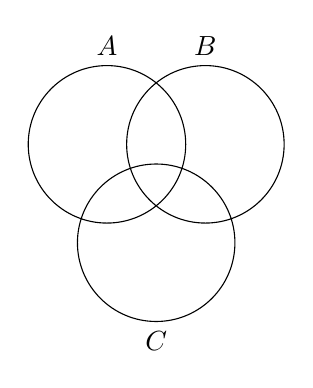
\begin{tikzpicture}[fill=gray]
            \def\bx{1.25}
            \def\cy{-1.25}
            \def\circA{(0,0) circle (1)}
            \def\circB{(\bx,0) circle (1)}
            \def\circC{(\bx/2,\cy) circle (1)}
            \def\vennrect{(-1,\cy-1) rectangle (\bx+1,1)}
            \def\@true{1}

            % A only
            \ifx1#1
                \begin{scope}
                    \clip \vennrect \circB;
                    \clip \vennrect \circC;
                    \fill \circA;
                \end{scope}
            \fi

            % B only
            \ifx1#2
                \begin{scope}
                    \clip \vennrect \circA;
                    \clip \vennrect \circC;
                    \fill \circB;
                \end{scope}
            \fi

            % C only
            \ifx1#3
                \begin{scope}
                    \clip \vennrect \circA;
                    \clip \vennrect \circB;
                    \fill \circC;
                \end{scope}
            \fi

            % A and B only
            \ifx1#4
                \begin{scope}
                    \clip \vennrect \circC;
                    \clip \circA;
                    \clip \circB;
                    \fill \circA;
                \end{scope}
            \fi

            % A and C only
            \ifx1#5
                \begin{scope}
                    \clip \vennrect \circB;
                    \clip \circA;
                    \clip \circC;
                    \fill \circA;
                \end{scope}
            \fi

            % B and C only
            \ifx1#6
                \begin{scope}
                    \clip \vennrect \circA;
                    \clip \circB;
                    \clip \circC;
                    \fill \circB;
                \end{scope}
            \fi

            % A and B and C
            \ifx1#7
                \begin{scope}
                    \clip \circA;
                    \clip \circB;
                    \clip \circC;
                    \fill \circA;
                \end{scope}
            \fi

            % Draw circles and labels
            \draw \circA (0,1)  node [text=black,above] {$A$}
            \circB (\bx,1)  node [text=black,above] {$B$}
            \circC (\bx/2,\cy-1)  node [text=black,below] {$C$};
        \end{tikzpicture}
    \end{center}
}
\newcommand\venndiagii[3]{
    \begin{center}
        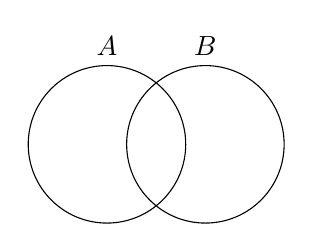
\begin{tikzpicture}[fill=gray]
            \def\bx{1.25}
            \def\circA{(0,0) circle (1)}
            \def\circB{(\bx,0) circle (1)}
            \def\vennrect{(-1,-1) rectangle (\bx+1,1)}
            \def\@true{1}

            % A only
            \ifx1#1
                \begin{scope}
                    \clip \vennrect \circB;
                    \fill \circA;
                \end{scope}
            \fi

            % B only
            \ifx1#2
                \begin{scope}
                    \clip \vennrect \circA;
                    \fill \circB;
                \end{scope}
            \fi

            % A and B only
            \ifx1#3
                \begin{scope}
                    \clip \circA;
                    \clip \circB;
                    \fill \circA;
                \end{scope}
            \fi

            % Draw circles and labels
            \draw \circA (0,1)  node [text=black,above] {$A$}
            \circB (\bx,1)  node [text=black,above] {$B$};
        \end{tikzpicture}
    \end{center}
}

\exercise{1}{
    Prove all the displayed formulas in this section and visualize them using Venn diagrams.
}
\sol{
    \newcommand*{\comproof}[2]{
        \ali{
            x \in A #1 B &\bic x \in A #2 x \in B \\
            &\bic x \in B #2 x \in A \\
            &\bic x \in B #1 A,
        }
    }
    \newcommand*{\assocproof}[2]{
        \ali{
            (A #1 B ) #1 C &\bic x \in A #1 B #2 x \in C \\
            &\bic (x \in A #2 x \in B) #2 x \in C \\
            &\bic x \in A #2 x \in B #2 x \in C \\
            &\bic x \in A #2 (x \in B #2 x \in C) \\
            &\bic x \in A #2 x \in B #1 C \\
            &\bic x \in A #1 (B #1 C),
        }
    }
    For commutivity, Venn diagrams are not very useful.
    \qproof{
        For all $x$, we have that
        \comproof{\cap}{\land}
        which shows that $A \cap B = B \cap A$.
        Similarly, we have that
        \comproof{\cup}{\lor}
        which proves that $A \cup B = B \cup A$.
    }

    Venn diagrams also provide no insight for associativity.
    \qproof{
        Again, for any $x$, we have that
        \assocproof{\cap}{\land}
        showing that $(A \cap B) \cap C = A \cap (B \cap C)$.
        Likewise, we have
        \assocproof{\cup}{\lor}
        and hence $(A \cup B) \cup C = A \cup (B \cup C)$.
    }

    \newcommand*{\distproof}[4]{
        \ali{
            x \in A #1 (B #2 C) &\bic x \in A #3 (x \in B #4 x \in C) \\
            &\bic (x \in A #3 x \in B) #4 (x \in A #3 x \in C) \\
            &\bic x \in A #1 B #4 x \in A #1 C \\
            &\bic x \in (A #1 B) #2 (A #1 C),
        }
    }
    For distributivity, Venn diagrams \emph{do} provide insight.
    The Venn diagram for the distributive identity $A \cap (B \cup C) = (A \cap B) \cup (A \cap C)$ is shown below:
    \venndiagiii{0}{0}{0}{1}{1}{0}{1}
    A proof of this follows directly from the distributivity of logical conjunction.
    \qproof{
        For all $x$, we have
        \distproof{\cap}{\cup}{\land}{\lor}
        which proves the result.
    }
    Likewise, the Venn diagram for $A \cup (B \cap C) = (A \cup B) \cap (A \cup C)$ is shown below:
    \venndiagiii{1}{0}{0}{1}{1}{1}{1}
    This time, the proof follows directly from the distributivity of logical disjunction.
    \qproof{
        For every $x$, we have that
        \distproof{\cup}{\cap}{\lor}{\land}
        proving the desired result.
    }

    \newcommand\demorgproof[4]{
        \ali{
            x \in C - (A #1 B) &\bic x \in C \land x \notin A #1 B \\
            &\bic x \in C \land \lnot (x \in A #1 B) \\
            &\bic x \in C \land \lnot (x \in A #2 x \in B) \\
            &\bic x \in C \land (x \notin A #3 x \notin B) \\
            &\bic (x \in C \land x \notin A) #3 (x \in C \land x \notin B) \\
            &\bic x \in C - A #3 x \in C - B \\
            &\bic x \in (C - A) #4 (C - B),
        }
    }
    Regarding the two DeMorgan laws, proofs of these rely on the DeMorgan and distributive laws of logic.
    First, we have $C - (A \cap B) = (C - A) \cup (C - B)$:
    \venndiagiii{0}{0}{1}{0}{1}{1}{0}
    \qproof{
        For all $x$,
        \demorgproof{\cap}{\land}{\lor}{\cup}
        of course showing the result.
    }
    The other DeMorgan law is of course $C - (A \cup B) = (C - A) \cap (C - B)$:
    \venndiagiii{0}{0}{1}{0}{0}{0}{0}
    \qproof{
        Again, for all $x$, we have
        \demorgproof{\cup}{\lor}{\land}{\cap}
        which proves the result.
    }

    Next, we have the property $A \cap (B - C) = (A \cap B) - C$, which is visualized below:
    \venndiagiii{0}{0}{0}{1}{0}{0}{0}
    The proof of this follows from the associativity of logical conjunction.
    \qproof{
        For all $x$, we have
        \ali{
            x \in A \cap (B - C) &\bic x \in A \land x \in B - C \\
            &\bic x \in A \land (x \in B \land x \notin C) \\
            &\bic (x \in A \land x \in B) \land x \notin C \\
            &\bic x \in A \cap B \land x \notin C \\
            &\bic x \in (A \cap B) - C,
        }
        showing the result.
    }

    The next claim is that $A - B = \es$ if and only if $A \ss B$, for which a Venn diagram is not useful.
    \qproof{
        \bicproof{
            First suppose that $A - B = \es$ and consider any $x \in A$.
            Suppose that $x \notin B$.
            Then we would have $x \in A$ but $x \notin B$ so that $x \in A - B$, contradicting the fact that $A - B = \es$.
            Hence, it has to be that $x \in B$ so that $A \ss B$ since $x$ was arbitrary.
        }{
            Now suppose that $A \ss B$ but that $A - B \neq \es$ so that there is an  $x \in A - B$.
            Therefore, $x \in A$ but $x \notin B$.
            However, since $A \ss B$ it must also be that $x \in B$ since $x \in A$, a contradiction!
            So it in fact has to be that $A - B = \es$ as desired.
        }
    }

    To prove the next property, it is first useful to establish the following lemma.
    \begin{lem}
        For any set $A$, $A - A = \es$.
    \end{lem}
    \qproof{
        This is very nearly self-evident, but suppose $A - A \neq \es$ so that there is an $x \in A - A$.
        Then it would both be true that $x \in A$ and $x \notin A$.
        As this is a clear contradiction, it has to be that in fact $A - A = \es$ as claimed.
    }
    The next property is then that $A \sd A = \es$, for which again a Venn diagram provides no insight and in fact does not really even make sense.
    \qproof{
        By definition and the above lemma,
        \gath{
            A \sd A = (A - A) \cup (A - A) = \es \cup \es = \es.
        }
        Clearly $\es \cup \es = \es$ since, were there an $x \in \es \cup \es$, we would have $x \in \es$ or $x \in \es$, the same impossibility in either case.
    }

    The penultimate property asserted in this section is that $A \sd B = B \sd A$.
    \qproof{
        This follows trivially from the commutativity of the union operation, proven above.
        By definition, we simply have
        \gath{
            A \sd B = (A - B) \cup (B - A) = (B - A) \cup (A - B) = B \sd A.
        }
    }

    The final property is $(A \sd B) \sd C = A \sd (B \sd C)$, i.e. that the symmetric difference operation is associative.
    This set is visualized below:
    \venndiagiii{1}{1}{1}{0}{0}{0}{1}
    In order to prove this while avoiding great tedium, we introduce the logical ``exclusive or'' operation, also called XOR.
    The reader may already have some familiarity with this operation, but for propositions $P$ and $Q$, we denote the XOR of $P$ and $Q$ as $P \lxor Q$.
    The XOR operation is defined by the following truth table:
    \begin{center}
        \begin{tabular}{cc|c}
            $P$ & $Q$ & $P \lxor Q$ \\
            \hline
            F   & F   & F           \\
            F   & T   & T           \\
            T   & F   & T           \\
            T   & T   & F
        \end{tabular}
    \end{center}
    \begin{lem}\label{lem:oper:xorid}
        We claim the logical identity $P \lxor Q \bic (P \land \lnot Q) \lor (Q \land \lnot P)$
    \end{lem}
    \qproof{
        To prove this, we work out the truth table for the right-hand side, in which we set $R = (P \land \lnot Q) \lor (Q \land \lnot P)$ for brevity:
        \begin{center}
            \begin{tabular}{cc|cc|cc|c}
                $P$ & $Q$ & $\lnot P$ & $\lnot Q$ & $P \land \lnot Q$ & $Q \land \lnot P$ & $R$ \\
                \hline
                F   & F   & T         & T         & F                 & F                 & F   \\
                F   & T   & T         & F         & F                 & T                 & T   \\
                T   & F   & F         & T         & T                 & F                 & T   \\
                T   & T   & F         & F         & F                 & F                 & F
            \end{tabular}
        \end{center}
        Since the truth table for $R$ is identical to that for $P \lxor Q$ above, this proves the identity.
    }
    \begin{lem}\label{lem:oper:xorassoc}
        The logical XOR operation is associative, that is that $(P \lxor Q) \lxor R \bic P \lxor (Q \lxor R)$.
    \end{lem}
    \qproof{
        This is again most easily proved via exhaustive truth tables:
        \begin{center}
            \begin{tabular}{ccc|c|c}
                $P$ & $Q$ & $R$ & $P \lxor Q$ & $(P \lxor Q) \lxor R$ \\
                \hline
                F   & F   & F   & F           & F                     \\
                F   & F   & T   & F           & T                     \\
                F   & T   & F   & T           & T                     \\
                F   & T   & T   & T           & F                     \\
                T   & F   & F   & T           & T                     \\
                T   & F   & T   & T           & F                     \\
                T   & T   & F   & F           & F                     \\
                T   & T   & T   & F           & T
            \end{tabular}
        \end{center}
        \pagebreak
        \begin{center}
            \begin{tabular}{ccc|c|c}
                $P$ & $Q$ & $R$ & $Q \lxor R$ & $P \lxor (Q \lxor R)$ \\
                \hline
                F   & F   & F   & F           & F                     \\
                F   & F   & T   & T           & T                     \\
                F   & T   & F   & T           & T                     \\
                F   & T   & T   & F           & F                     \\
                T   & F   & F   & F           & T                     \\
                T   & F   & T   & T           & F                     \\
                T   & T   & F   & T           & F                     \\
                T   & T   & T   & F           & T
            \end{tabular}
        \end{center}
        Since the final column of both tables are identical, this shows the desired result.
    }
    \begin{lem}\label{lem:oper:sdxor}
        For sets $A$ and $B$ and any $x$, $x \in A \sd B$ if and only if $x \in A \lxor x \in B$.
    \end{lem}
    \qproof{
        For any $x$, define the proposition $P$ as $x \in A$ and $Q$ as $x \in B$.
        Then we have that
        \ali{
            x \in A \sd B &\bic x \in (A -  B) \cup (B - A) & \text{Definition of $\sd$} \\
            &\bic x \in A - B \lor x \in B - A & \text{Definition of union} \\
            &\bic (x \in A \land x \notin B) \lor (x \in B \land x \notin A) & \text{Definition of set difference} \\
            &\bic (P \land \lnot Q) \lor (Q \land \lnot P) & \text{Definitions of $P$ and $Q$} \\
            &\bic P \lxor Q & \text{Lemma~\ref{lem:oper:xorid}} \\
            &\bic x \in A \lxor x \in B, & \text{Definitions of $P$ and $Q$}
        }
        which of course proves the result.
    }
    Finally, we are ready to prove the original assertion that the symmetric difference is associative.
    \qproof{
        For any $x$, define the proposition $P$ as $x \in A$, $Q$ as $x \in B$ and $R$ as $x \in C$.
        We then have that
        \ali{
            x \in (A \sd B) \sd C &\bic (x \in A \lxor x \in B) \lxor x \in C & \text{Lemma~\ref{lem:oper:sdxor}} \\
            &\bic (P \lxor Q) \lxor R & \text{Definitions of $P$, $Q$, and $R$} \\
            &\bic P \lxor (Q \lxor R) & \text{Lemma~\ref{lem:oper:xorassoc}} \\
            &\bic x \in A \lxor (x \in B \lxor x \in C) & \text{Definitions of $P$, $Q$, and $R$} \\
            &\bic x \in A \sd (B \sd C). & \text{Lemma~\ref{lem:oper:sdxor}}
        }
        This of course suffices to show that $(A \sd B) \sd C = A \sd (B \sd C)$.
    }
}

\exercise{2}{
    Prove:
    \begin{enumerate}
        \item[(a)] $A \ss B$ if and only if $A \cap B = A$ if and only if $A \cup B = B$ if and only if $A - B = \es$.
        \item[(b)] $A \ss B \cap C$ if and only if $A \ss B$ and $A \ss C$.
        \item[(c)] $B \cup C \ss A$ if and only if $B \ss A$ and $C \ss A$.
        \item[(d)] $A - B = (A \cup B) -B = A - (A \cap B)$.
        \item[(e)] $A \cap B = A - (A - B)$.
        \item[(f)] $A - (B - C) = (A - B) \cup (A \cap C)$.
        \item[(g)] $A = B$ if and only if $A \sd B = \es$.
    \end{enumerate}
}
\sol{
    (a) \qproof{
        \bicproof{
            First assume that $A \ss B$.

            To show that $A \cap B = A$, first consider $x \in A \cap B$, then clearly $x \in A$ so that $A \cap B \ss A$.
            Now suppose that $x \in A$ so that also $x \in B$ since $A \ss B$.
            Hence, $x \in A$ and $x \in B$ so that $x \in A \cap B$, showing that $A \ss A \cap B$.

            Next we show that $A \cup B = B$.
            First consider any $x \in A \cup B$.
            If $x \in A$ then also $x \in B$ since $A \ss B$.
            Since, in the other case, we have that $x \in B$ directly, it follows that $A \cup B \ss B$.
            Now suppose that $x \in B$ so that clearly also $x \in A \cup B$, and so $B \ss A \cup B$ as well.

            Finally, we show that $A - B = \es$.
            To see this, assume first that $A - B \neq \es$ so that there is an $x \in A - B$.
            Thus, $x \in A$ but $x \notin B$.
            However, $x \in A$ implies that $x \in B$ since $A \ss B$, which is a contradiction.
        }{
            First suppose that $A \cap B = A$ and consider any $x \in A$ so that also $x \in A \cap B$, and hence $x \in B$ as well.
            This shows that $A \ss B$.

            Next, suppose that $A \cup B = B$ and consider any $x \in A$.
            Then $x \in A \cup B = B$, which suffices to show that $x \in B$ and thus $A \ss B$.

            Lastly, suppose that $A - B = \es$ and consider any $x \in A$.
            Were it the case that $x \notin B$ then it would follow that $x \in A - B = \es$, an impossibility.
            Hence, it has to be that $x \in B$ as well so that $A \ss B$ again.
        }

        This all suffices to show that
        \gath{
            A \ss B \bic A \cap B = A \bic A \cup B = B \bic A - B = \es
        }
        as desired.
    }

    (b) \qproof{
        \bicproof{
            Suppose first that $A \ss B \cap C$ and consider any $x \in A$.
            Then also $x \in B \cap C$ so that both $x \in B$ and $x \in C$.
            As $x$ was arbitrary, this shows that both $A \ss B$ and $A \ss C$.
        }{
            Now suppose that $A \ss B$ and $A \ss C$ and consider any $x \in A$.
            Then both $x \in B$ since $A \ss B$, and $x \in C$ since $A \ss C$.
            Therefore, $x \in B \cap C$, showing that $A \ss B \cap C$.
        }
    }

    (c) \qproof{
        \bicproof{
            First suppose that $B \cup C \ss A$ and consider any $x \in B$.
            Then $x \in B \cup C$ so that also $x \in A$, showing that $B \ss A$.
            Similarly, for any $x \in C$ we have that again $x \in B \cup C$ so that $x \in A$.
            This shows that $C \ss A$ as well.
        }{
            Now suppose that both $B \ss A$ and $C \ss A$ and consider any $x \in B \cup C$.
            In the case in which $x \in B$, we have that $x \in A$ since $B \ss A$.
            In the other case in which $x \in C$ we also have $x \in A$ since $C \ss A$ as well.
            This shows that $B \cup C \ss A$ since $x$ was arbitrary.
        }
    }

    (d) \qproof{
        \seteqproof{
            Suppose that $x \in A - B$ so that $x \in A$ and $x \notin B$.
            Then of course also $x \in A \cup B$ since $x \in A$.
            Since also $x \notin B$ it follows that $x \in (A \cup B) - B$, showing that $A - B \ss (A \cup B) - B$.
            We also have that $x \notin A \cap B$ since $x \notin B$.
            Hence, also $x \in A - (A \cap B)$ so that $A - B \ss A - (A \cap B)$ as well.
        }{
            Suppose that $x \in (A \cup B) - B$.
            Then $x \in A \cup B$ and $x \notin B$.
            Since it must be that $x \in A$ or $x \in B$, but $x \notin B$, it must be that $x \in A$.
            Hence, $x \in A - B$, which proves that $(A \cup B) - B \ss A - B$.

            Now suppose that $x \in A - (A \cap B)$ so that $x \in A$ and $x \notin A \cap B$.
            Since $x \in A$ it has to be that $x \notin B$ since otherwise it would be that $x \in A \cap B$.
            Therefore, $x \in A$ and $x \notin B$ so that $x \in A - B$, showing that also $A - (A \cap B) \ss A - B$.

            This all is sufficient to show that
            \gath{
                A - B = (A \cup B) - B = A - (A \cap B)
            }
            as desired.
        }
    }

    (e) First, a somewhat obvious lemma.
    \begin{lem}\label{lem:oper:negsd}
        For any $x$, $x$ is \emph{not} a member of $A - B$ if and only if $x \notin A$ or $x \in B$.
    \end{lem}
    \qproof{
        This is shown with some basic rules of logic.
        For any $x$, we have
        \ali{
            x \notin A - B &\bic \lnot(x \in A - B) & \\
            &\bic \lnot(x \in A \land x \notin B) & \text{Definition of set difference} \\
            &\bic x \notin \lor x \in B, & \text{DeMorgan law for logical conjunction}
        }
        and it is as simple as that.
    }
    Now we can prove the desired result.
    \qproof{
        Consider any $x$.
        Let $F$ be the proposition that $x \in A$ and $x \notin A$, which is of course \emph{always} false.
        We then have
        \ali{
            x \in A \cap B &\bic x \in A \land x \in B & \text{Definition of set intersection} \\
            &\bic F \lor (x \in A \land x \in B) & \text{Since $F$ is always false} \\
            &\bic (x \in A \land x \notin A) \lor (x \in A \land x \in B) & \text{Definition of $F$} \\
            &\bic x \in A \land (x \notin A \lor x \in B) & \text{Distributive law for conjunction} \\
            &\bic x \in A \land x \notin A - B & \text{Lemma~\ref{lem:oper:negsd}} \\
            &\bic x \in A - (A - B), & \text{Definition of set difference}
        }
        showing the desired result.
    }

    (f) \qproof{
        Here we have, for any $x$,
        \ali{
            x \in A - (B - C) &\bic x \in A \land x \notin B - C & \text{Definition of set difference} \\
            &\bic x \in A \land (x \notin B \lor x \in C) & \text{Lemma~\ref{lem:oper:negsd}} \\
            &\bic (x \in A \land x \notin B) \lor (x \in A \land X \in C) & \text{Distributive law for conjunction} \\
            &\bic x \in A - B \lor x \in A \cap C & \text{Definitions of $-$ and $\cap$} \\
            &\bic x \in (A - B) \cup (A \cap C), & \text{Definition of set union}
        }
        which proves the result.
    }

    (g) \qproof{
        \bicproof{
            Suppose that $A = B$.
            Then $A \sd B = A \sd A = \es$ by a property of the symmetric difference that was listed in the text and proven in Exercise~1.4.1 above.
        }{
            Now suppose that $A \sd B = \es$.
            Then it follows that both $A - B = \es$ and $B - A = \es$ since otherwise we would have that $A \sd B = (A - B) \cup (B - A) \neq \es$.

            Now consider any $x \in A$ so that of course $x \notin A - B = \es$.
            Then, by Lemma~\ref{lem:oper:negsd}, we have that $x \notin A$ or $x \in B$.
            Hence, $x \in B$ since we have already established that $x \in A$.
            This shows that $A \ss B$.

            Now consider any $x \in B$ so that, similarly, $x \notin B - A = \es$.
            Then, again by Lemma~\ref{lem:oper:negsd}, $x \notin B$ or $x \in A$ so that $x \in A$ since $x \in B$.
            This shows that $B \ss A$ as well, and therefore that $A = B$ as desired.
        }
    }
}

\exercise{3}{
    For each of the following (false) statements draw a Venn diagram in which it fails:
    \begin{enumerate}
        \item[(a)] $A - B = B - A$.
        \item[(b)] $A \cap B \pss A$.
        \item[(c)] $A \ss B \cup C$ implies $A \ss B$ or $A \ss C$.
        \item[(d)] $B \cap C \ss A$ implies $B \ss A$ or $C \ss A$.
    \end{enumerate}
}
\sol{
    (a) The following is an arrangement of $A$ and $B$ the demonstrates the falsehood:
    \venndiagii{0}{0}{0}
    In particular, $A - B$ is
    \venndiagii{1}{0}{0}
    while $B - A$ is
    \venndiagii{0}{1}{0}
    which are clearly not equal.

    (b) This is demonstrated by the following sets:
    \begin{center}
        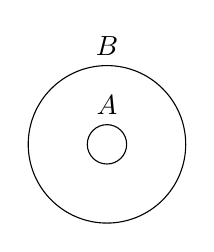
\begin{tikzpicture}
            \draw (0,0) circle (1) (0,1)  node [text=black,above] {$B$};
            \draw (0,0) circle (0.25) (0,0.25)  node [text=black,above] {$A$};
        \end{tikzpicture}
    \end{center}
    Here $A \ss B$ so that $A \cap B = A$, and hence $A \cap B$ is not a \emph{proper} subset of $A$.

    (c) Sets that contradict this assertion are shown below, in which $A$ is shaded:
    \begin{center}
        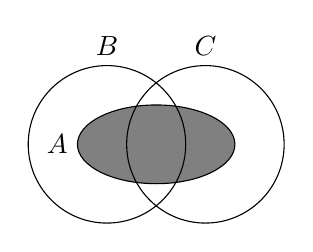
\begin{tikzpicture}
            \def\cx{1.25}
            \draw[fill=gray] (\cx/2,0) ellipse (1 and 0.5) (\cx/2-1,0) node [text=black,left] {$A$};
            \draw (0,0) circle (1) (0,1)  node [text=black,above] {$B$};
            \draw (\cx,0) circle (1) (\cx,1)  node [text=black,above] {$C$};
        \end{tikzpicture}
    \end{center}
    Here clearly $A$ is a subset of $B$ and $C$ taken together (i.e. $B \cup C$), but also clearly is a subset of neither $B$ nor $C$ alone.

    (d) Here is an example of sets that contradict this assertion, in which $B \cap C$ is shaded:
    \begin{center}
        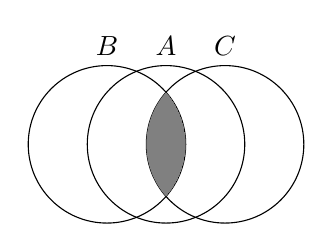
\begin{tikzpicture}[fill=gray]
            \def\cx{1.5}
            \def\circB{(0,0) circle (1)}
            \def\circC{(\cx,0) circle (1) (\cx,1)}
            \draw \circB (0,1)  node [text=black,above] {$B$};
            \draw \circC  node [text=black,above] {$C$};
            \draw (\cx/2,0) circle (1) (\cx/2,1) node [text=black,above] {$A$};

            % Shade B cap C
            \begin{scope}
                \clip \circB;
                \clip \circC;
                \fill \circB;
            \end{scope}
        \end{tikzpicture}
    \end{center}
    Clearly $B \cap C$ is a subset of $A$, but neither B not C alone are subsets of $A$.
}

\exercise{4}{
    Let $A$ be a set; show that a ``complement'' of $A$ does not exist.
    (The ``complement'' of $A$ is the set of all $x \notin A$.)
}
\sol{
    TODO
}

\exercise{5}{
    Let $S \neq \es$ and $A$ be sets.
    \begin{enumerate}
        \item[(a)] Set $T_1 = \braces{Y \in \pset{A} \where \text{$Y = A \cap X$ for some $X \in S$}}$, and prove $A \cap \bigcup S = \bigcup T_1$ (generalized distributive law).
        \item[(b)] Set $T_2 = \braces{Y \in \pset{A} \where \text{$Y = A - X$ for some $X \in S$}}$, and prove
            \gath{
                A - \bigcup S = \bigcap T_2 \\
                A - \bigcap S = \bigcup T_2
            }
            (generalized De Morgan's laws).
    \end{enumerate}
}
\sol{
    TODO
}

\exercise{6}{
    Prove that $\bigcap S$ exists for all $S \neq \es$.
    Where s the assumption that $S \neq \es$ used in the proof?
}
\sol{
    TODO
}

  \setcounter{section}{5-1}

  \section{Cardinal Numbers}
  \subsection{Cardinal Arithmetic}

\exercise{1}{
  Prove properties (a)-(n) of cardinal arithmetic stated in the text of this section.
  These are

  (a) $\k + \l = \l + \k$

  (b) $\k + (\l + \mu) = (\k + \l) + \mu$

  (c) $\k \leq \k + \l$

  (d) If $\k_1 \leq \k_2$ and $\l_1 \leq \l_2$, then $\k_1 + \l_1 \leq \k_2 + \l_2$

  (e) $\k \cdot \l = \l \cdot \k$

  (f) $\k \cdot (\l \cdot \mu) = (\k \cdot \l) \cdot \mu$

  (g) $\k \cdot (\l + \mu) = \k \cdot \l + \k \cdot \mu$

  (h) $\k \leq \k \cdot \l$ if $\l > 0$

  (i) If $\k_1 \leq \k_2$ and $\l_1 \leq \l_2$, then $\k_1 \cdot \l_1 \leq \k_2 \cdot \l_2$

  (j) $\k + \k = 2 \cdot \k$

  (k) $\k + \k \leq \k \cdot \k$, whenever $\k \geq 2$

  (l) $\k \leq \k^\l$ if $\l > 0$

  (m) $\l \leq \k^\l$ if $\k > 1$

  (n) If $\k_1 \leq \k_2$ and $\l_1 \leq \l_2$, then $\k_1^{\l_1} \leq \k_2^{\l_1}$
}
\sol{
For solutions (a) through (c) suppose that
\ali{
  \k &= |K|  &
  \l &= |L| &
  \mu &= |M|,
}
where $K$, $L$, and $M$ are mutually disjoint sets.

(a)
\qproof{
  It is obvious that
  $$
    \k + \l = |K \cup L| = |L \cup K| = \l + \k
  $$
  since $K \cup L = L \cup K$ and $K$ and $L$ are disjoint.
}

(b)
\qproof{
  First we note that clearly
  $$
    K \cup (L \cup M) = K \cup L \cup M = (K \cup L) \cup M.
  $$
  Now suppose that there is an $x \in K \cap (L \cup M)$ so that $x \in K$ and $x \in L \cup M$
  If $x \in L$ then $x \in K \cap L$ and if $x \in M$ then $x \in K \cap M$, either of which is a contradiction since all three sets are mutually disjoint.
  Hence $K$ and $L \cup M$ are disjoint.
  A similar argument show that $K \cup L$ and $M$ are disjoint.
  Thus we have the following:
  $$
    \k + (\l + \mu) = |K| + |L \cup M| = |K \cup (L \cup M)| = |(K \cup L) \cup M| = |K \cup L| + |M| = (\k + \l) + \mu
  $$
  as desired.
}

(c)
\qproof{
  Define the function $f: K \to K \cup L$ by simply the identity $f(k) = k$ for any $k \in K$.
  Obviously this is an injective function so that $\k = |K| \leq |K \cup L| = \k + \l$.
}

(d)
\qproof{
  Suppose that
  \ali{
    \k_1 &= |K_1| &
    \k_2 &= |K_2| &
    \l_1 &= |L_1| &
    \l_2 &= |L_2|
  }
  for sets $K_1$, $K_2$, $L_1$, and $L_2$ where $K_1 \cap L_1 = \es$ and $K_2 \cap L_2 = \es$.
  Also suppose that $\k_1 \leq \k_2$ and $\l_1 \leq \l_2$.
  Thus $|K_1| = \k_1 \leq \k_2 = |K_2|$ so that there is an injective function $f$ from $K_1$ to $K_2$.
  Similarly there is an injective function $g : L_1 \to L_2$ since $|L_1| = \l_1 \leq \l_2 = |L_2|$.
  Now define $h : K_1 \cup L_1 \to K_2 \cup L_2$ by
  $$
    h(x) = \begin{cases}
      f(x) & x \in K_1  \\
      g(x) & x \in L_1.
    \end{cases}
  $$
  We show that $h$ is injective so consider $x$ and $y$ in $K_1 \cup L_1$ where $x \neq y$.

  Case: $x \in K_1$, $y \in K_1$.
  Then
  $$
    h(x) = f(x) \neq f(y) = h(y)
  $$
  since $f$ is injective and $x \neq y$.

  Case: $x \in L_1$, $y \in L_1$.
  Then
  $$
    h(x) = g(x) \neq g(y) = h(y)
  $$
  since $g$ is injective and $x \neq y$.

  Case: $x \in K_1$, $y \in L_1$.
  Then we have $h(x) = f(x) \in K_2$ and $h(y) = g(y) \in L_2$ so that $h(x) \neq h(y)$ since $K_2$ and $L_2$ are disjoint.
  Note that this is the same as the case in which $x \in L_1$ and $y \in K_1$ since we simply switch $x$ and $y$.

  Since these cases are exhaustive and $h(x) \neq h(y)$ in each this shows that $h$ is injective.
  Hence we have demonstrated that
  $$
    \k_1 + \l_1 = |K_1 \cup L_1| \leq |K_2 \cup L_2| = \k_2 + \l_2
  $$
  as desired.
}

For solutions (e) through (h) suppose that
\ali{
  \k &= |A| & \l &= |B| & \mu &= |C|
}
for sets $A$, $B$, and $C$.

(e)
\qproof{
  First we show that $|A \times B| = |B \times A|$ by constructing a bijection $f : A \times B \to B \times A$.
  For $(a,b) \in A \times B$ define
  $$
    f(a,b) = (b,a) \in B \times A,
  $$
  which is clearly a function.
  Then for $(a,b) \in A \times B$ and $(c,d) \in A \times B$ where $f(a,b) = f(c,d)$ we have
  $$
    f(a,b) = (b,a) = f(c,d) = (d,c)
  $$
  so that $b=d$ and $a=c$.
  Hence $(a,b) = (c,d)$ so that $f$ is injective.
  Now consider any $(b,a) \in B \times A$ so that clearly $f(a,b) = (b,a)$, noting that $(a,b) \in A \times B$.
  Clearly this shows that $f$ is surjective.

  Hence $f$ is bijective so that
  $$
    \k \cdot \l = |A \times B| = |B \times A| = \l \cdot \k
  $$
  as required.
}

(f)
\qproof{
  Similar part (e) above, it is trivial to find a bijection from $A \times (B \times C)$ to $(A \times B) \times C$ so that
  $$
    \k \cdot (\l \cdot \mu) = |A \times (B \times C)| = |(A \times B) \times C| = (\k \cdot \l) \cdot \mu
  $$
  as desired.
}

(g)
\qproof{
  Here suppose additionally that $B \cap C = \es$.
  First we note that since $B$ and $C$ are disjoint that $A \times B$ and $A \times C$ are also disjoint.
  Suppose that this is not the case so that there is an $(a,b) \in A \times B$ where $(a,b) \in A \times C$ also.
  Then clearly $b \in B$ and $b \in C$, which is a contradiction since they are disjoint.
  Now, it is also trivial to show the equality
  $$
    A \times (B \cup C) = (A \times B) \cup (A \times C).
  $$
  Hence we have that
  $$
    \k \cdot (\l + \mu) = \k \cdot |B \cup C| = |A \times (B \cup C)| = |(A \times B) \cup (A \times C)|
    = |A \times B| + |A \times C| = \k \cdot \l + \k \cdot \mu
  $$
  as desired.
}

(h)
\qproof{
  Here suppose that $\l > 0$  so that $B \neq \es$.
  Here we construct a bijection $f: A \to A \times B$, from which it follows that
  $$
    \k = |A| \leq |A \times B| = \k \cdot \l.
  $$
  Since $B \neq \es$ there exists a $b \in B$.
  So for any $a \in A$ define
  $$
    f(a) = (a, b),
  $$
  which is clearly a function.
  So for $a_1, a_2 \in A$ where $a_1 \neq a_2$ we have that
  $$
    f(a_1) = (a_1, b) \neq (a_2, b) = f(a_2)
  $$
  so that $f$ is injective.
}

(i)
\qproof{
  Suppose that
  \ali{
    \k_1 &= |A_1| & \k_2 &= |A_2| & \l_1 &= |B_1| & \l_2 &= |B_2|
  }
  for sets $A_1$, $A_2$, $B_1$, and $B_2$ where $\k_1 = |A_1| \leq |A_2| = \k_2$ and $\l_1 = |B_1| \leq |B_2| = \l_2$.
  Hence there is an injective function $f: A_1 \to A_2$ and injective function $g: B_1 \to B_2$.
  We shall construct an injective function $h: A_1 \times B_1 \to A_2 \times B_2$ so that it immediately follows that
  $$
    \k_1 \cdot \l_1 = |A_1 \times B_1| \leq |A_2 \times B_2| = \k_2 \cdot \l_2
  $$
  as required.
  So for $(a, b) \in A_1 \times B_1$ define
  $$
    h(a, b) = (f(a), g(b))
  $$
  Suppose then $(a, b) \in A_1 \times B_1$ and $(c, d) \in A_1 \times B_1$ where $(a,b) \neq (c,d)$.
  If $a \neq c$ then $f(a) \neq f(c)$ since $f$ is injective so that
  $$
    h(a,b) = (f(a), g(b)) \neq (f(c), g(d)) = h(c,d)
  $$
  Similarly if $b \neq d$ then $g(b) \neq g(d)$ since $g$ is injective.
  Hence again
  $$
    h(a,b) = (f(a), g(b)) \neq (f(c), g(d)) = h(c,d)
  $$
  Thus in all cases $h(a,b) \neq h(c,d)$ so that $h$ is injective.
}

(j) This is adequately proven in the text.

For solutions (k) through (m) suppose that
\ali{
  \k &= |A| & \l &= |B|
}
for sets $A$ and $B$.

(k)
\qproof{
  Suppose here that $\k \geq 2$.
  Then $2 \leq \k$ and $\k \leq \k$ so that by property (i) we have
  $$
    2 \cdot \k \leq \k \cdot \k.
  $$
  Then by property (j) we have
  $$
    \k + \k = 2 \cdot \k \leq \k \cdot \k
  $$
  as desired.
}

(l)
\qproof{
  Here suppose that $\l = |B| > 0$ so that $B \neq \es$.
  Hence there exists a $b \in B$.
  We shall construct an injective $f: A \to A^B$, from which it follows that
  $$
    \k = |A| \leq |A^B| = \k^\l.
  $$
  So for any $a \in A$ define $f(a) = g$ where $g : B \to A$ is a function defined by $g(b) = a$ for all $b \in B$, noting that $g \neq \es$ since $B \neq \es$.

  Now consider any $a_1, a_2 \in A$ where $a_1 \neq a_2$ so that for any $b \in B$ we have
  $$
    f(a_1)(b) = a_1 \neq a_2 = f(a_2)(b).
  $$
  From this it follows that $f(a_1) \neq f(a_2)$ so that $f$ is injective.
}

(m)
\qproof{
  Here suppose that $\k = |A| > 1$ so that there are $a_1, a_2 \in A$ where $a_1 \neq a_2$.
  We shall construct an injective function $f: B  \to A^B$ so that
  $$
    \l = |B| \leq |A^B| = \k^\l.
  $$
  So for any $b \in B$ define $f(b) = g$ where $g: B \to A$ is a function defined by
  $$
    g(c) =
    \begin{cases}
      a_1 & c = b    \\
      a_2 & c \neq b
    \end{cases}
  $$
  for $c \in B$.
  Now suppose that $b_1, b_2 \in B$ where $b_1 \neq b_2$.
  We then have
  $$
    f(b_1)(b_1) = a_1 \neq a_2 = f(b_2)(b_1)
  $$
  since $b_1 \neq b_2$.
  From this it follows that $f(b_1) \neq f(b_2)$ so that $f$ is injective.
}

(n)
\qproof{
Suppose that
\ali{
  \k_1 &= |A_1| & \k_2 &= |A_2| & \l_1 &= |B_1| & \l_2 &= |B_2|
}
for sets $A_1$, $A_2$, $B_1$, and $B_2$ where $\k_1 = |A_1| \leq |A_2| = \k_2$ and $\l_1 = |B_1| \leq |B_2| = \l_2$.

The theorem as presented in the text is actually not true in full generality.
As a counterexample suppose that $A_1 = A_2 = B_1 = \es$ so that $\k_1 = \k_2 = \l_1 = 0$ and $B_2 = 1$ so that $\l_2 = 1$.
Then certainly the hypotheses above are true but we also have
$$
  \k_1^{\l_1} = 0^0 = 1 > 0 = 0^1 = \k_2^{\l_2}
$$
where we have used the results of Exercises~5.1.2 and 5.1.3.

However, if we add the restriction that $\k_2 > 0$ then it becomes true.
To prove this first note that this implies that $A_2 \neq \es$ so that there is an $a_2 \in A_2$.
Also there is an injective function $f: A_1 \to A_2$ and an injective function $g: B_1 \to B_2$.
We shall construct an injective $F: A_1^{B_1} \to A_2^{B_2}$, from which it follows that
$$
  \k_1^{\l_1} = |A_1^{B_1}| \leq |A_2^{B_2}| = \k_2^{\l_2}.
$$
So for any $h_1 \in A_1^{B_1}$ define $F(h_1) = h_2$ where $h_2 \in A_2^{B_2}$ is defined by
$$
  h_2(b) = \begin{cases}
    f(h_1(g^{-1}(b))) & b \in \ran(h_1)    \\
    a_2               & b \notin \ran(h_1)
  \end{cases}
$$
for any $b \in B_2$, noting that $g^{-1}$ is a function on $\ran(h_1)$ since $g$ is injective.
Clearly $F$ is a function but now we show that it is injective.

So consider any $h_1, h_2 \in A_1^{B_1}$ where $h_1 \neq h_2$.
Then there is a $b_1 \in B_1$ such that $h_1(b_1) \neq h_2(b_1)$.
So let $b_2 = g(b_1)$ so that clearly $b_2 \in \ran(g)$ and $b_1 = g^{-1}(b_2)$.
Hence we have
$$
  F(h_1)(b_2) = f(h_1(g^{-1}(b_2))) = f(h_1(b_1)) \neq f(h_2(b_1)) = f(h_2(g^{-1}(b_2))) = F(h_2)(b_2)
$$
since $h_1(b_1) \neq h_2(b_1)$ and $f$ is injective.
It thus follows that $F(h_1) \neq F(h_2)$ so that we have shown that $F$ is injective.
}
}

\exercise{2}{
  Show that $\k^0 = 1$ and $\k^1 = \k$ for all $\k$.
}
\sol{
  \qproof{
    Suppose that $\k = |A|$ for a set $A$.

    We claim that $A^\es = \braces{\es} = 1$ so that clearly
    $$
      \k^0 = |A^\es| = |1| = 1.
    $$
    First consider any $f \in A^\es$.
    Suppose that $f \neq \es$ so that there is a $(b,a) \in f \subseteq \es \times A$.
    But then $b \in \es$, which is a contradiction.
    Hence $f = \es$.
    So if there are any $f \in A^\es$ then $f = \es$ but are there any $f \in A^\es$?
    Clearly the empty set is a function from $\es$ to $A$ since it is vacuously true that for every $b \in \es$ there is a unique $a \in A$ such that $(b,a) \in \es$.
    Hence $\es \in A^\es$ so that $A^\es = \braces{\es} = 1$.

    We also claim that $|A^1| = |A|$ so that
    $$
      \k^1 = |A^1| = |A| = \k.
    $$
    To this end for any $f \in A^1$ define $F(f) = f(\es)$, noting that $1 = \braces{\es}$, so that clearly $F: A^1 \to A$.
    Now consider any $f,g \in A^1$ where $f \neq g$.
    Then it has to be that
    $$
      F(f) = f(\es) \neq g(\es) = F(g)
    $$
    so that $F$ is injective.
    Now consider any $a \in A$ and define $f \in A^1$ by $f(\es) = a$.
    Then clearly
    $$
      F(f) = f(\es) = a
    $$
    so that $F$ is surjective.
    Hence we've shown that $F$ is bijective.
  }
}

\exercise{3}{
  Show that $1^\k = 1$ for all $\k$ and $0^\k = 0$ for all $\k > 0$.
}
\sol{
  \qproof{
    Suppose that $\k = |A|$ for a set $A$.

    Note first that if $\k = 0$ then by Exercise~5.1.2 it follows that
    $$
      1^\k = 1^0 = 1.
    $$
    In the case where $\k > 0$ we claim that there is a unique $f \in 1^A$ so that clearly then
    $$
      1^\k = |1^A| = 1.
    $$
    For existence define $f:A \to 1$ by $f(x) = \es$ for all $x \in A$ so that clearly $f \in 1^A$.
    For uniqueness consider any $f_1, f_2 \in 1^A$.
    Since $1 = \braces{\es}$ it has to be that $f_1(x) = f_2(x) = \es$ for all $x \in A$.
    Hence $f_1 = f_2$.

    Now suppose also that $\k > 0$ so that $A \neq \es$.
    Hence there is an $a \in A$.
    We claim that in this case that $\es^A = \es$ so that
    $$
      0^\k = |\es^A| = |\es| = 0.
    $$
    So suppose that $\es^A \neq \es$ so that there \emph{is} an $f \in \es^A$.
    Then it's true that for every $a \in A$ there is a unique $b \in \es$ such that $f(a) = b$.
    But since there \emph{is} an $a \in A$ this implies that there is also a $b \in \es$, which is a contradiction.
    Hence there can be no $f \in \es^A$ so that $\es^A = \es$.
  }
}

\exercise{4}{
  Prove that $\k^\k \leq 2^{\k \cdot \k}$.
}
\sol{
\qproof{
Suppose that $\k = |A|$ for a set $A$.
Then we construct an injective $F : A^A \to 2^{A \times A}$ so that
$$
  \k^\k = |A^A| \leq |2^{A \times A}| = |2|^{|A \times A|} = 2^{\k \cdot \k}.
$$
So for any $f \in A^A$ define $F(f) = g$ where $g \in 2^{A\times A}$ is defined by
$$
  g(a_1, a_2) =
  \begin{cases}
    0 & f(a_1) \neq a_2 \\
    1 & f(a_1) = a_2
  \end{cases}
$$
for $(a_1, a_2) \in A \times A$.
To show that $F$ is injective consider any $f,g \in A^A$ where $f \neq g$.
Then there is an $a \in A$ such that $f(a) \neq g(a)$.
Now let $a_1 = f(a)$ and $a_2 = g(a)$ so that
$$
  f(a) = a_1 \neq a_2 = g(a).
$$
Since $f(a) = a_1$ it follows by definition that $F(f)(a,a_1) = 1$.
Similarly since $g(a) = a_2  \neq a_1$ it follows that $F(g)(a,a_1) = 0$.
Hence we have
$$
  F(f)(a, a_1) = 1 \neq 0 = F(g)(a, a_1)
$$
so that clearly $F(f) \neq F(g)$.
Thus $F$ is injective.
}
}

\exercise{5}{
  If $\abs{A} \leq \abs{B}$ and if $A \neq \es$, then there is a mapping of $B$ onto $A$.
  We later show, with the help of the Axiom of Choice, that the converse is also true: If there is a mapping of $B$ onto $A$, then $\abs{A} \leq \abs{B}$.
}
\sol{
  \qproof{
    Suppose that $|A| \leq |B|$ for sets $A$ and $B$ where $A \neq \es$.
    Then there is an $a \in A$.
    There is also an injective $f : A \to B$ so that $f^{-1}$ is a function from $\ran(f) \to A$.
    So let $g$ be a mapping from $B$ to $A$ defined by
    $$
      g(b) = \begin{cases}
        f^{-1}(b) & b \in \ran(f)     \\
        a         & b \notin \ran(f).
      \end{cases}
    $$
    To show that $g$ is onto consider any $x \in A$ and let $b = f(a)$. Thus $b \in \ran(f)$ so that
    $$
      g(b) = f^{-1}(b) = f^{-1}(f(a)) = a.
    $$
    Hence $g$ is onto since $a$ was arbitrary.
  }
}

\exercise{6} {
  If there is a mapping of $B$ onto $A$, then $2^{\abs{A}} \leq 2^{\abs{B}}$.
    [Hint: Given $g$ mapping $B$ onto $A$, let $f(X) = \inv{g}[X]$, for all $X \ss A$.]
}
\sol{
\qproof{
Suppose that $f$ is a mapping from $B$ \emph{onto} $A$.
We shall construct an injective $F: 2^A \to 2^B$ so that
$$
  2^{|A|} = |2|^{|A|} = |2^A| \leq |2^B| = |2|^{|B|} = 2^{|B|}.
$$
So for any $g \in 2^A$ let $F(g) = h$ where $h \in 2^B$ is defined by
$$
  h(b) = g(f(b))
$$
for $b \in B$.
To show that $F$ is injective consider any $g_1, g_2 \in 2^A$ where $g_1 \neq g_2$.
Then there is an $a \in A$ such that $g_1(a) \neq g_2(a)$.
Since $f : B \to A$ is onto there is a $b \in B$ such that $f(b) = a$.
Thus we have
$$
  F(g_1)(b) = g_1(f(b)) = g_1(a) \neq g_2(a) = g_2(f(b)) = F(g_2)(b)
$$
so that $F(g_1) \neq F(g_2)$.
Thus $F$ is injective.
}
}

\exercise{7}{
  Use Cantor's Theorem to show that ``the set of all sets'' does not exist.
}
\sol{
  \qproof{
    Suppose that $X$ is the set of all sets.
    Consider any $Z \in \pset{X}$.
    Since clearly $Z$ is a set we have $Z \in X$.
    Thus since $Z$ was arbitrary it follows that $\pset{X} \subseteq X$ so that by Exercise~4.1.3 $|\pset{X}| \leq |X|$.
    However, this contradicts Cantor's Theorem, according to which $|\pset{X}| > |X|$.
    Thus $X$ cannot be the set of all sets.
  }
}

\exercise{8}{
  Let $X$ be a set and let $f$ be a one-to-one mapping of $X$ into itself such that $f[X] \pss X$.
  Then $X$ is infinite.
}
\sol{
  \qproof{
    For a set $X$ suppose that $f : X \to X$ is injective.
    Also suppose that $\ran(f)$ is a proper subset of $X$.

    Now suppose that $X$ is finite so that there is an $n \in \nats$ such that there is a bijective $g : n \to X$.
    We also note that clearly $g^{-1} : X \to n$ is also a bijection.
    Now define a function $h : n \to n$ by
    $$
      h(k) = (g^{-1} \circ f \circ g)(k) = g^{-1}(f(g(k))
    $$
    for any $k \in n$.
    Since $g$, $f$, and $g^{-1}$ are all injective it follows from Exercise~2.3.5 that $h$ is also injective.

    We now claim that $\ran(h)$ is proper subset of $n$.
    First we note that for any $m \in n$ we have
    $$
      g(h(m)) = g(g^{-1}(f(g(m)))) = f(g(m))
    $$
    since $g$ is a function.
    Now, since $\ran(f) \subset X$ there is an $x \in X$ such that $x \notin \ran(f)$.
    So let $k = g^{-1}(x)$ so that $g(k) = x$.
    Now suppose that there is an $m \in n$ such that $h(m) = k$.
    Then per the above we have
    $$
      f(g(m)) = g(h(m)) = g(k) = x,
    $$
    which is impossible since $x \notin \ran(f)$.
    So it must be that there is no such $m$ so that $k \notin \ran(h)$
    Hence since $k \in n$ it follows that $\ran(g) \subset n$.

    Now clearly $h$ is a surjective mapping from $n$ to $\ran(h)$.
    But since $h$ is also injective it is thus a bijection from $n$ to $\ran(n)$.
    However, according to Lemma~4.2.2 there is no bijective mapping from $n$ to $\ran(n)$ since $\ran(h) \subset n$.
    We have thus arrived at a contradiction so that, if the hypotheses hold, then $X$ cannot be finite.
    Hence by definition $X$ is infinite.
  }
}

\exercise{9}{
  Every countable set is Dedekind infinite.
}
\sol{
\begin{lem}\label{lem:card:equidede}
  If sets $X$ and $Y$ are equipotent (i.e. $|X| = |Y|$) and $Y$ is Dedekind infinite then $X$ is also Dedekind infinite.
\end{lem}
\qproof{
Since $X$ and $Y$ are equipotent there is a bijective $f : X \to Y$ so that $\inv{f}$ is also bijective.
Also since $Y$ is Dedekind infinite there is a $Z \subset Y$ such that there is a bijective $g : Y \to Z$ so that $\inv{g}$ is also bijective.
So since $Z \subset Y$ there is a $y \in Y$ such that $y \notin Z$.
So let $S = X - \braces{\inv{f}(y)}$.
Clearly since $\inv{f}(y) \in X$ it follows that $S \subset X$ since $\inv{f}(y) \notin S$.
Now define $h: X \to S$ by
$$
  h(x) = (\inv{f} \circ g \circ f)(x) = \inv{f}(g(f(x))))
$$
for $x \in X$.
Since $f$ is a function this implies that
$$
  f(h(x)) = f(\inv{f}(g(f(x)))) = g(f(x)).
$$
Now suppose for a moment that there is an $x \in X$ such that $h(x) = \inv{f}(y)$.
Then
$$
  g(f(x)) = f(h(x)) = f(\inv{f}(y)) = y,
$$
which is impossible since $y \notin Z$ but $\ran(g) \subseteq Z$.
Hence there is no such $x$ so that $h$ really is a map from $X$ to $S$ (as opposed to $X$ to $X$).

Now, since $\inv{f}$, $g$, and $f$ are all injective it follows from Exercise~2.3.5 that $h$ is injective as well.
Then consider any $s \in S$ and let $x = \inv{f}(\inv{g}(f(s)))$, noting that $\inv{g}(f(s))$ exists since $s \neq \inv{f}(y)$.
Then we have
$$
h(x) = \inv{f}(g(f(\inv{f}(\inv{g}(f(s))))))) = \inv{f}(g(\inv{g}(f(s)))) = \inv{f}(f(s)) = s
$$
so that $h$ is surjective since $s$ was arbitrary.
Hence $h$ is a bijective map from $X$ to $S$, and since $S \subset X$ this means that $X$ is Dedekind infinite.
}

\begin{lem}\label{lem:card:natdede}
  $\nats$ is Dedekind infinite.
\end{lem}
\qproof{
  Let $N = \nats - \braces{0}$ so that clearly $N$ is proper subset of $\nats$.
  Then we define the map $f : \nats \to N$ by
  $$
    f(n) = n+1
  $$
  for $n \in \nats$.
  Consider any $n,m \in \nats$ where $n \neq m$.
  Then clearly
  \gath{
    n \neq m \\
    n+1 \neq m+1 \\
    f(n) \neq f(m)
  }
  so that $f$ is injective.
  Now consider any $n \in N$ so that clearly $f(n-1) = (n-1) + 1 = n$, noting that since $n \neq 0$ we have $n \geq 1$ so that $n-1 \geq 0$.
  Hence $n-1 \in \nats$.
  This shows that $f$ is surjective.
  Hence $f$ is a bijection from $\nats$ onto a proper subset $N$ so that by definition $\nats$ is Dedekind infinite.
}

\mainprob
\qproof{
  Suppose that $X$ is a countable set.
  Then by definition $X$ is equipotent to $\nats$.
  Hence since $\nats$ is Dedekind infinite (Lemma~\ref{lem:card:natdede}) it follows that $X$ is as well by Lemma~\ref{lem:card:equidede}.
}
}

\exercise{10}{
  If $X$ contains a countable subset, then $X$ is Dedekind infinite.
}
\sol{
  \qproof{
    Suppose that $X$ is a set with a countable subset $Y$.
    Then by Exercise~5.1.9 $Y$ is Dedekind infinite so that there is a $Z \subset Y \subseteq X$ such that there is a bijective $f : Y \to Z$.
    So define the following $g: X \to X$ by
    $$
      g(x) = \begin{cases}
        f(x) & x \in Y    \\
        x    & x \notin Y
      \end{cases}
    $$
    for any $x \in X$.
    Now since $Z \subset Y$ there is a $y \in Y$ such that $y \notin Z$, noting that since $Y \subseteq X$, $y \in X$.

    First we claim that $y \notin \ran(g)$.
    So suppose that it is so that there is an $x \in X$ such that $g(x) = y$.
    If $x \in Y$ then by definition $g(x) = f(x) = y$, but this is a contradiction since $f : Y \to Z$ but $y \notin Z$.
    On the other hand if $x \notin Y$ then we have $g(x) = x = y$, which is also a contradiction since $y = x \in Y$.
    Since a contradiction follows in either case it must be that there is no such $x$ so that $y \notin \ran(g)$.
    Hence $\ran(g) \subset X$.

    Clearly $g$ is a surjective map from $X$ to $\ran(g)$ so we now show that it is injective.
    So consider any $x_1, x_2 \in X$ where $x_1 \neq x_2$.

    Case: $x_1 \in Y$ and $x_2 \in Y$.
    Then
    $$
      g(x_1) = f(x_1) \neq f(x_2) = g(x_2)
    $$
    since $f$ is injective.

    Case: $x_1 \notin Y$ and $x_2 \notin Y$.
    Then
    $$
      g(x_1) = x_1 \neq x_2 = g(x_2).
    $$

    Case: $x_1 \in Y$ and $x_2 \notin Y$.
    Then $g(x_1) = f(x_1) \in Z$ but $g(x_2) = x_2 \notin Y$ so that  $x_2 \notin Z$ either since $Z \subset Y$.
    Hence $f(x_1) \neq x_2$ so that
    $$
      g(x_1) = f(x_1) \neq x_2 = g(x_2).
    $$
    Thus in all cases $g(x_1) \neq g(x_2)$ so that $g$ is injective since $x_1$ and $x_2$ were arbitrary.

    Therefore we have shown that $g$ is a bijective map from $X$ to $\ran(g) \subset X$ so that $X$ is Dedekind infinite by definition.
  }
}

\exercise{11}{
  If $X$ is Dedekind infinite, then it contains a countable subset.
    [Hint: Let $x \in X - f[X]$; define $x_0 = x$, $x_1 = f(x_0)$, \ldots, $x_{n+1} = f(x_n)$, \ldots.
      The set $\braces{x_n \where n \in \nats}$ is countable.]
}
\sol{
  \qproof{
    Suppose that $X$ is a Dedekind infinite set.
    Then there is a $Y \subset X$ such that there is a bijective $f : X \to Y$.
    Since $Y \subset X$ there is an $x \in X$ such that $x \notin Y$.
    So first define $x_0 = x$ and then for $n \in \nats$ define $x_{n+1} = f(x_n)$.

    We claim that $x_n \neq x_m$ for any $n,m \in \nats$ where $n \neq m$, from which it clearly follows that
    $$
      Z = \braces{x_n \where n \in \nats}
    $$
    is a countable set.
    So consider any $n,m \in \nats$ where $n \neq m$
    Without loss of generality we can assume that $n < m$.
    Suppose that  $x_n = x_m$.
    We now show by induction that $x_{n-k} = x_{m-k}$ for all $n \geq k \geq 0$.
    If $k=0$ then we clearly have
    $$
      x_{n-k} = x_{n-0} = x_n = x_m = x_{m-0} = x_{m-k}.
    $$
    Now suppose that $x_{n-k} = x_{m-k}$.
    We then have
    $$
      f(x_{n-(k+1)}) = f(x_{n-k-1}) = x_{n-k} = x_{m-k} = f(x_{m-k-1}) = f(x_{m-(k+1)})
    $$
    Since $f$ is injective this implies that $x_{n-(k+1)} = x_{m-(k+1)}$ so that inductive proof is complete.
    So since this holds for $k=n$ we have that
    $$
      x_0 = x_{n-n} = x_{m-n} = f(x_{m-n-1}),
    $$
    Noting that $m-n-1 \geq 0$ since $m \geq n +1$.
    But $x_0 = x \notin Y$ and $f(x_{m-n-1}) \in Y$ since $f:X \to Y$ so that we have a contradiction.
    So it must be that $x_n \neq x_m$.
    Hence $Z$ is countable.
    Since also clearly $Z \subseteq X$ the proof is complete.
  }
}

\exercise{12}{
  If $A$ and $B$ are Dedekind infinite, the $A \cup B$ is Dedekind infinite.
    [Hint: Use Exercise~1.11.]
}
\sol{
  \qproof{
    Suppose that sets $A$ and $B$ are both Dedekind infinite.
    Then $A$ contains a countable subset $C$ by Exercise~5.1.11.
    Clearly $C \subseteq A \cup B$ so that $C$ is a countable subset of $A \cup B$.
    Hence by Exercise~5.1.10 $A \cup B$ is Dedekind infinite.
  }
}

\exercise{13}{
  If $A$ and $B$ are Dedekind infinite, then $A \times B$ is Dedekind infinite.
    [Hint: Use Exercise~1.11.]
}
\sol{
  \qproof{
    Suppose that $A$ and $B$ are both Dedekind infinite.
    Then $A$ contains a countable subset $C$ by Exercise~5.1.11.
    Also since $B$ is Dedekind infinite it is not finite by Exercise~5.1.8.
    Hence $B \neq \es$ so that there is a $b \in B$.
    Clearly then the set
    $$
      D = \braces{(a,b) \where a \in C}
    $$
    is a countable subset of $A \times B$ so that $A \times B$ is Dedekind infinite by Exercise~5.1.10.
  }
}

\exercise{14}{
  If $A$ is infinite, then $\pset{\pset{A}}$ is Dedekind infinite.
    [Hint: For each $n \in \nats$, let $S_n = \braces{X \pss A \where \abs{X} = n}$.
      The set $\braces{S_n \where n \in \nats}$ is a countable subset of $\pset{\pset{A}}$.]
}
\sol{
  \begin{lem}\label{lem:card:infss}
    If $A$ is an infinite set then for any $n \in \nats$ there is a $B \subseteq A$ such that $|B| = n$.
  \end{lem}
  \qproof{
    Suppose that $A$ is an infinite set and consider any $n \in \nats$.
    Then $\cnats \leq |A|$ so that there is an injective $f : \nats \to A$.
    Now $n \in \nats$ but also $n \subseteq \nats$.
    So define the set
    $$
      B = \braces{f(k) \where k \in n}.
    $$
    Clearly $B \subseteq A$ and we show that $|B| = n$ by defining a mapping $g : n \to B$ by
    $$
      g(k) = f(k)
    $$
    for $k \in n$.
    Since $f$ is injective clearly $g$ is.
    Now consider any $b \in B$.
    By definition then there is a $k \in n$ such that $f(k) = b$.
    Hence $g(k) = f(k) = b$ so that $g$ is surjective.
    Hence since $g$ is bijective $|B| = n$ as desired.
  }

  \mainprob
  \qproof{
    Suppose that $A$ is infinite.
    Then for any $n \in \nats$ define
    $$
      S_n = \braces{X \in \pset{A} \where |X| = n},
    $$
    noting that $S_n \neq \es$ by Lemma~\ref{lem:card:infss}.
    We also note that for $n,m \in \nats$ where $n \neq m$ we have $S_n \neq S_m$ since for any $X \in S_n$ and $Y \in S_m$ we have
    $$
      |X| = n \neq m = |Y|
    $$
    so that $X \neq Y$.
    From this it follows that
    $$
      S = \braces{S_n \where n \in \nats}
    $$
    is a countable set.
    Also, for an $S_n \in S$ we have that each $X \in S_n$ is in $\pset{A}$ so that $S_n \subseteq \pset{A}$.
    Hence each $S_n \in \pset{\pset{A}}$.
    Thus $S \subseteq \pset{\pset{A}}$.
    Since $S$ is countable it then follows that $\pset{\pset{A}}$ is Dedekind infinite by Exercise~5.1.10.
  }
}

  \subsection{The Cardinality of the Continuum}

\exercise{1}{
  Prove that the set of all finite sets of reals has cardinality $2^{\al_0}$.
  We remark here that the set of all countable sets of reals also has cardinality $2^{\al_0}$, but the proof of this requires the Axiom of Choice.
}
\sol{
  \qproof{
    Let $F$ denote the set of all finite sets of reals.
    First we construct an injective $f: F \to \reals^\nats$
    So consider any $A \in F$.
    Then $|A|=n$ for an $n \in \nats$ so that there is a finite sequence $\angles{a_k \where k \in n}$ where $\ran(a) = A$.
    Now we define an infinite sequence of reals $\hat{a} \in \reals^\nats$ by
    $$
      \hat{a}_k = \begin{cases}
        a_k & k \in n\, \text{(i.e. $0 \leq k < n$)} \\
        a_0 & k \notin n\, \text{(i.e. $k \geq n$)}
      \end{cases}
    $$
    so that clearly we have $\ran(\hat{a}) = A$ as well.
    Note that this only works if $A \neq \es$ since otherwise there is no $a_0$.
    In the case  where $A = \es$ we set $\hat{a}_k = k$ for $k \in \nats$ so that $\ran(\hat{a}) = \nats$.
    In any case we set $f(A) = \hat{a}$.

    Now we claim that $f$ is injective.
    So consider any $A,B \in F$ where $A \neq B$.
    If one of them is the empty set, say $A$, then since $B$ is finite $m = \max(\ceil{\max(B)} + 1, 0)$ exists so that clearly $m \notin B$.
    Hence $m \notin \ran(f(B)) = B$.
    However $m \in \ran(f(A)) = \nats$ since $m \in \nats$.
    It thus follows that $\ran(f(B)) \neq \ran(f(A))$ so that $f(A) \neq f(B)$.
    On the other hand if neither $A$ nor $B$ is the empty set (but still $A \neq B$) then there is an $a \in A$ where $a \notin B$ or vice versa.
    Without loss of generality we need only consider the first case.
    Clearly then $a \in \ran(f(A)) = A$ but $a \notin \ran(f(B)) = B$ so that again $f(A) \neq f(B)$.
    Hence in all cases we've shown that $f$ is injective.

    Thus we have that
    $$
      |F| \leq |\reals^\nats| = \ccont,
    $$
    where the last equality was shown in Theorem~5.2.3d.
    Now define
    $$
      E = \braces{\braces{x} \where x \in \reals}
    $$
    so that clearly $E \subseteq F$ and $|E| = |\reals|$.
    Hence we have
    $$
      \ccont = |\reals| = |E| \leq |F|
    $$
    by Exercise 4.1.3.
    Thus by the \cbthrm{} $|F| = \ccont$ as required.
  }
}

\exercise{2}{
  A real number $x$ is \emph{algebraic} if it is a solution of some equation
  $$
    a_n x^n + a_{n-1} x^{n-1} + \cdots + a_1 x + a_0 = 0,
  $$
  where $a_0, \ldots, a_n$ are integers.
  If $x$ is not algebraic, it is called \emph{transcendental}.
  Show that the set of algebraic numbers is countable and hence the set of all transcendental numbers has cardinality $2^{\al_0}$.
}
\sol{
  I did not prove this here as I have already done so when studying Rudin's Principles of Mathematical Analysis, Exercise~2.2.
}

\exercise{3}{
  If a linearly ordered set $P$ has a countable dense subset, then $\abs{P} \leq 2^{\al_0}$.
}
\sol{
  Note that the countable dense subset is dense in $P$ and not just in itself as explained in the errata list.
  \qproof{
    Suppose that $(P,<)$ is our linearly ordered set and $R$ is the countable dense subset of $P$.
    We construct an $f : P \to \pset{R}$ by defining
    $$
      f(x) = \braces{y \in R \where y < x}
    $$
    for any $x \in P$.
    Clearly for such $x$ we have that $f(x) \ss R$ so that $f(x) \in \pset{R}$.

    Now we claim that $f$ is injective.
    So consider any $x,y \in P$ such that $x \neq y$.
    Without loss of generality we can assume that $x < y$.
    Since $R$ is dense in $P$ there is a $z \in R$ where $x < z < y$.
    From this it follows that $z \in f(y)$ but that $z \notin f(x)$ since it is not true that $z < x$.
    Hence clearly $f(x) \neq f(y)$ so that we have shown that $f$ is injective.

    Thus we have
    $$
      |P| \leq |\pset{R}| = 2^{|R|} = \ccont,
    $$
    where we have  used Theorem~5.1.9.
  }
}

\exercise{4}{
  The set of all closed subsets of reals has cardinality $2^{\al_0}$.
}
\sol{
  \qproof{
    Let $C$ denote all the closed subsets of $\reals$ and $O$ the open sets.
    We form a mapping $f: C \to O$ defined by
    $$
      f(A) = \reals - A
    $$
    for $A \in C$.
    Clearly by definition $f(A)$ is open for every $A \in C$ since $A$ is closed.

    Now consider any $A,B \in C$ where $A \neq B$.
    Then there is an $a \in A$ such that $a \notin B$ or vice versa.
    Without loss of generality we can assume the former.
    Then since $a \in A$ it follows that $a \notin \reals - A$.
    But also since $a \notin B$ (but $a \in \reals$) we have that $a \in \reals - B$.
    Thus
    $$
      f(A) = \reals - A \neq \reals - B = f(B)
    $$
    so that $f$ is injective.

    Now consider any $B \in O$ and let $A = \reals - B$.
    $$
      f(A) = \reals - A = \reals - (\reals - B) = B
    $$
    so that $f$ is also surjective.
    Hence we have that
    $$
      |C| = |O| = \ccont
    $$
    by Theorem~2.6b.
  }
}

\exercise{5}{
  Show that, for $n > 0$, $n \cdot 2^\ccont = \cnats \cdot 2^\ccont = \ccont \cdot 2^\ccont = 2^\ccont \cdot 2^\ccont = \parens{2^\ccont}^n = \parens{2^\ccont}^\cnats = \parens{2^\ccont}^\ccont = 2^\ccont$.
}
\sol{
  \begin{lem}\label{lem:card:multone}
    For any cardinal number $\k$
    $$
      1 \cdot \k = \k.
    $$
  \end{lem}
  \qproof{
    Suppose that $\k = |A|$ for a set $A$.
    We define $f : A \to 1 \times A$ by
    $$
      f(a) = (0, a)
    $$
    for $a \in A$, noting that $1 = \braces{0}$.
    Clearly by simple inspection this is bijective so that
    $$
      1 \cdot \k = |1 \times A| = |A| = \k
    $$
    as desired.
  }

  \mainprob
  \qproof{
    First we note that clearly since $\cnats \leq \ccont$ we have
    $$
      \ccont \leq 2^\ccont
    $$
    by property (n) in section~5.1.
    So consider any cardinal $n \in \nats$ where $n > 0$ so that $1 \leq n$.
    We then have
    \ali{
      2^\ccont &= 1 \cdot 2^\ccont & \text{(by Lemma~\ref{lem:card:multone})} \\
      &\leq n \cdot 2^\ccont \leq \cnats \cdot 2^\ccont \leq \ccont \cdot 2^\ccont \leq 2^\ccont \cdot 2^\ccont & \text{(repeated property (i) of 5.1)} \\
      &= \parens{2^\ccont}^2 & \text{(by property (o) of 5.1)}\\
      &= 2^{2 \cdot \ccont} & \text{(by Theorem 5.1.7b)} \\
      &= 2^\ccont. & \text{(by Theorem 5.2.2b)}
    }
    We also have
    \ali{
      2^\ccont &= \parens{2^\ccont}^1 & \text{(by Exercise 5.1.2)} \\
      &\leq \parens{2^\ccont}^n \leq \parens{2^\ccont}^\cnats \leq \parens{2^\ccont}^\ccont & \text{(repeated property (n) of 5.1)} \\
      &= 2^{\ccont \cdot \ccont} & \text{(by Theorem 5.1.7b)} \\
      &= 2^\ccont & \text{(by Theorem 5.2.2b)}
    }
    Clearly these together with the \cbthrm{} shows the desired result.
  }
}

\exercise{6}{
  The cardinality of the set of all discontinuous functions is $2^\ccont$.
    [Hint: Using Exercise~2.5, show that $\abs{\reals^\reals - C} = 2^\ccont$ whenever $\abs{C} \leq \ccont$.]
}
\sol{
  \begin{lem}\label{lem:card:contminus}
    If $B$ is a set with $|B| = 2^\ccont$ and $A$ is a subset of $B$ with $|A| \leq \ccont$ then $|B - A| = 2^\ccont$.
  \end{lem}
  \qproof{
    The proof is analogous to that of Theorem~5.2.4.
    So suppose that $C$ is a set with $|C| = 2^\ccont$.
    Let $B = C \times C$ so that by Exercise~5.2.5 we have
    $$
      |B| = |C \times C| = 2^\ccont \cdot 2^\ccont = 2^\ccont.
    $$
    Also suppose that $A \subseteq B$ where $|A| = \ccont$.
    Now define a set
    $$
      P = \braces{x \in C \where \exists y \in C ((x,y) \in A)}.
    $$
    Clearly then $|P| \leq |A| = \ccont$.
    Since also $|C| = 2^\ccont$ but $P \subseteq C$ it follows that there is an $x_0 \in C$ where $x_0 \notin P$.
    If we let $X = \braces{x_0} \times C$ then any $(x,y) \in X$ is not in $A$ so that $(x,y) \in C\times C - A = B - A$.
    Hence $X \subseteq B - A$ but also since there is an obvious bijection between $X$ and $C$ we have
    $$
      2^\ccont = |C| = |X| \leq |B-A|.
    $$
    Since also clearly $B - A \subseteq B$ we also have that
    $$
      |B-A| \leq |B| = 2^\ccont.
    $$
    Hence by the \cbthrm{} $|B-A| = 2^\ccont$ as desired.
  }

  \mainprob
  \qproof{
    By Lemma~5.2.7 $|\reals^\reals| = 2^\ccont$.
    Also by Theorem~5.2.6a the set $C$ of all continuous $f: \reals \to \reals$ has cardinality of $\ccont$.
    Thus clearly the set of all discontinuous functions from $\reals \to \reals$ is simply
    $$
      D = \reals^\reals - C.
    $$
    But then by Lemma~\ref{lem:card:contminus} above we have that
    $$
      |D| = |\reals^\reals| = 2^\ccont
    $$
    as desired.
  }
}

\exercise{7}{
  Construct a one-to-one mapping of $\reals \times \reals$ onto $\reals$.
    [Hint: If $a,b \in [0, 1]$ have decimal expansions $0.a_1 a_2 a_3 \cdots$ and $0.b_1 b_2 b_3 \cdots$, map the ordered pair $(a,b)$ onto $0.a_1 b_1 a_2 b_2 a_3 b_3 \cdots \in [0,1]$.
      Make adjustments to avoid sequences where the digit 9 appears from some place onward.]
}
\sol{
  Skipping this problem due to the obviousness of it in principle but the fact that the details are tedious, and I have proved similar problems when studying Rudin's Principles of Mathematical Analysis.
}


  \section{Ordinal Numbers}
  \subsection{Well-Ordered Sets}

\exercise{1}{
  Give an example of a linearly ordered set $(L,<)$ and an initial segment $S$ of $L$ which is not of the form $\braces{x \where x < a}$, for any $a \in L$.
}
\sol{
  We claim that $L = \reals$ and $S = \braces{x \in L \where x \leq 0}$ with the usual order meet the criteria.
  \qproof{
    First, clearly $L = \reals$ is a linearly ordered set.
    So consider any $a \in S$ and any $x < a$ so that we have
    $$
      x < a \leq 0.
    $$
    Hence $x \in S$ also so that by definition $S$ is an initial segment of $\reals$.
    Now suppose that $S$ does have the form
    $$
      S = \braces{x \in L \where x < a}
    $$
    for some $a \in L$.
    Since $0 \leq 0$ clearly $0 \in S$ by the original definition so that by the above $0 < a$.
    But now consider $a/2$, which is clearly in $L = \reals$.
    By the above $a/2 < a$ since $a > 0$ so $a/2 \in S$ but we also have $0 < a/2$ (hence it is not true that $a/2 \leq 0$) since $0 < a$ so that by the original definition $a/2 \notin S$.
    Since we have a contradiction it must be that $S$ cannot be expressed in such a form.
  }
}

\exercise{2}{
  $\w + 1$ is not isomorphic to $\w$ (in the well-ordering by $\in$).
}
\sol{
  \qproof{
    Since $\w = \nats$ and $\w + 1 = \w \cup \braces{\w}$ clearly $\w$ is a proper subset of $\w + 1$ (since $\w \notin \w$ but $\w \in \w + 1$).
    Now consider any $a \in \w = \nats$ and any $x < a$.
    Then clearly also $x \in \nats$ so $x \in \w$.
    Thus $\w$ is an initial segment of $\w + 1$.
    Then, since it has already been shown that both $\w$ and $\w + 1$ are well-ordered sets, it follows from Corollary~6.1.5a that they  cannot be isomorphic.
  }
}

\exercise{3}{
  There exist $\ccont$ well-orderings of the set of natural numbers.
}
\sol{
  \begin{lem}\label{lem:ord:isnats}
    Suppose that $A$ is a subset of $\nats$ (including $A = \nats$).
    Then every initial segment of $A$ with the standard ordering is finite.
  \end{lem}
  \qproof{
    Consider any initial segment $S$ of $(A, <)$.
    Then by Lemma~6.1.2 there is an $n \in A \ss \nats$ such that $S = \braces{k \in A \where k < n}$.
    So consider any $k \in S$ so that $k \in A \ss \nats$ and $k < n$.
    Then by the definition of $<$ we have that $k \in n$.
    Since $k$ was arbitrary this shows that $S \ss n$ so that $|S| \leq n$.
    From this it clearly follows that $S$ is finite since $n$ is.
  }

  \mainprob
  \qproof{
    Throughout the following let $<$ denote the standard well-ordering on $\nats$ and let $R$ be the set of all well-orderings defined on $\nats$.

    First we construct an injective $F: R \to \nats^\nats$.
    So for any $\prec \in R$ we have that $(\nats, <)$ and $(\nats, \prec)$ are two well-orderings of $\nats$.
    Consider then Theorem~6.1.3.
    We show that (c) cannot be the case, i.e. that an initial segment of $(\nats, <)$ cannot be isomorphic to $(\nats, \prec)$.
    So suppose that this is the case so that $f$ is an isomorphism from an initial segment $S$ of $(\nats, <)$ to $(\nats, \prec)$.
    Then by  Lemma~\ref{lem:ord:isnats}, $S$ is finite whereas $\nats$ is infinite, but since $f$ is a bijection this is impossible since it would imply that $|S| = |\nats| = \cnats$.
    Hence it must be that (a) $(\nats, <)$ is isomorphic to $(\nats, \prec)$ or (b) the former is isomorphic to an initial segment of the latter.
    In either case such an isomorphism $f$ is unique by Corollary~6.1.5c.
    So define $F(\prec) = f$, noting that clearly $f \in \nats^\nats$.

    Now we show that $F$ is injective by considering two $\prec_1, \prec_2 \in R$ where $\prec_1 \neq \prec_2$.
    Without loss of generality we can the assume that there is an $(n,m) \in \prec_1$ where $(n,m) \notin \prec_2$.
    Thus $n \prec_1 m$ but since $\prec_2$ is a linear, strict ordering and $\lnot (n \prec_2 m)$ it has to be that $m \prec_2 n$ since $n \neq m$.
    Now let $f_1 = F(\prec_1)$ and $f_2 = F(\prec_2)$.
    Since both $f_1$ and $f_2$ are bijective there are $k_1,l_1,k_2,l_2 \in \nats$ such that
    \ali{
      f_1(k_1) &= n & f_2(k_2) &= n \\
      f_1(l_1) &= m & f_2(l_2) &= m
    }
    Since $f_1$ is an isomorphism and $f_1(k_1) = n \prec_1 m = f_1(l_1)$ it follows that
    $$
      k_1 < l_1
    $$
    and similarly since $f_2$ is an isomorphism and $f_2(l_2) = m \prec_2 n = f_2(k_2)$ it follows that
    $$
      l_2 < k_2.
    $$
    Now we claim that either $f_1(k_1) \neq f_2(k_1)$ or $f_1(l_1) \neq f_2(l_1)$.
    Either case shows that $F(\prec_1) = f_1 \neq f_2 = F(\prec_2)$ so that $F$ is injective.
    To this end suppose that $f_1(k_1) = f_2(k_1) = n = f_2(k_2)$.
    Then since $f_2$ is injective it follows that $k_1 = k_2$.
    Hence with the above we have
    $$
      l_2 < k_2 = k_1 < l_1
    $$
    so that $m = f_2(l_2) \prec_2 f_2(l_1)$ and hence $m \neq f_2(l_1)$.
    Thus we have $f_1(l_1) = m \neq f_2(l_1)$ so that the disjunction is shown (since $\lnot P \to Q \equiv P \lor Q$) and $F$ is injective.

    Hence since $F: R \to \nats^\nats$ is injective we have that
    $$
      |R| \leq |\nats^\nats| = \cnats^\cnats = \ccont
    $$
    by Theorem~5.2.2c.

    Now suppose that $B$ is the set of all bijections from $\nats$ to $\nats$.
    We then construct an injective $G: 2^\nats \to B$.
    So for any infinite sequence $a \in 2^\nats$ we define an $f \in \nats^\nats$ by
    \ali{
      f(2n) &= \begin{cases}
        2n   & a_n = 0 \\
        2n+1 & a_n = 1
      \end{cases}
      &
      f(2n+1) &= \begin{cases}
        2n+1 & a_n = 0  \\
        2n   & a_n = 1.
      \end{cases}
    }
    for $n \in \nats$, i.e we swap $2n$ and $2n+1$ if $a_n = 1$ and leave them alone if $a_n = 0$.
    We then assign $G(a) = f$.
    It is trivial but tedious to show that $f$ is bijective so that indeed $f \in B$.

    Now consider any $a, b \in 2^\nats$ where $a \neq b$ and let $f = G(a)$ and $g = G(b)$.
    Since $a \neq b $ there is an $n \in \nats$ where $a_n \neq b_n$.
    Without loss of generality we can assume that $a_n = 0 \neq 1 = b_n$.
    Then we have
    $$
      f(2n) = 2n \neq 2n+1 = g(2n)
    $$
    since $a_1 = 0$ but $b_n = 1$.
    Hence $f \neq g$ so that $G$ is injective, from which it follows that $|2^\nats| \leq |B|$.

    Lastly we construct an injective $H : B \to R$.
    So for an $f \in B$ define
    $$
      \prec = \braces{(f(n), f(m)) \where (n,m) \in \nats \times \nats \land n < m}
    $$
    and set $H(f) = \prec$.
    Clearly by definition since $f$ is bijective it is an isomorphism from $(\nats, <)$ to $(\nats, \prec)$.
    This means that $(\nats, \prec)$ is isomorphic to $(\nats, <)$ so that clearly $\prec$ is a well-ordering since $<$ is.
    Hence indeed $H(f) = \prec \in R$.

    Now we show that $H$ is injective.
    So consider $f_1, f_2 \in B$ where $\prec_1 = H(f_1) = H(f_2) = \prec_2$.
    Then $\inv{f_1} \circ f_2$ is an isomorphism from $(\nats, \prec_1)$ to $(\nats, \prec_2)$
    But since $\prec_1 = \prec_2$ these are the same well-ordered set so that it follows from Corollary~6.1.5b that the only isomorphism between them is the identity $i_\nats$.
    Hence $\inv{f_1} \circ f_2 = i_\nats$, from which it follows that $f_1 = f_2$.
    Therefore $H$ is injective so that $|B| \leq |R|$.

    Putting this together results in
    $$
      \ccont = |2^\nats| \leq |B| \leq |R|.
    $$
    It then follows from the \cbthrm{} that $|R| = \ccont$ as desired.
  }
}

\exercise{4}{
  For every infinite subset $A$ of $\nats$, $(A,<)$ is isomorphic to $(\nats,<)$.
}
\sol{
  \qproof{
    Let $A$ be an infinite subset of $\nats$.
    Then $(A, <)$ (where $<$ is the standard well-ordering of $\nats$) is a well-ordering since any $B \ss A$ is also a subset of $\nats$ and therefore has a least element.
    Hence by Theorem~6.1.3 either:
    \begin{enumerate}
      \item $(A,<)$ and $(\nats,<)$ are isomorphic,
      \item An initial segment of $(A,<)$ is isomorphic to $(\nats,<)$, or
      \item $(A,<)$ is isomorphic to an initial segment of $(\nats,<)$
    \end{enumerate}
    We show that they must be isomorphic (1) by showing that (2) and (3) lead to contradictions.

    Suppose (2), i.e. that an initial segment $S$ of $(A,<)$ is isomorphic to $(\nats,<)$.
    Then since $A \ss \nats$ it follows from Lemma~\ref{lem:ord:isnats} that $S$ is finite.
    But since this is isomorphic to $\nats$ it means that $|S| = |\nats| = \cnats$, which is a contradiction!

    Now suppose (3) so that $(A,<)$ is isomorphic to an initial segment $S$ of $(\nats, <)$.
    Again Lemma~\ref{lem:ord:isnats} tells us that $S$ is finite whereas $A$ is infinite.
    But since they are isomorphic this implies that $|S| = |A| = \cnats$, which is again a contradiction!

    Hence it has to be that $(A,<)$ and $(\nats,<)$ are isomorphic.
  }
}

\exercise{5}{
  Let $(W_1, <_1)$ and $(W_2,<_2)$ be disjoint well-ordered sets, each isomorphic to $(\nats,<)$.
  Show that the sum of the two linearly ordered sets (as defined in Lemma~4.5 in Chapter~4) is a well-ordering, and is isomorphic to the ordinal number $\w + \w = \braces{0,1,2,\ldots,\w,\w+1,\w+2,\ldots}$.
}
\sol{
  \qproof{
    Suppose that $(W, \prec)$ is the sum and associated order as defined in Lemma~4.4.5.
    By that lemma $\prec$ is a linear ordering but we must show that it is also a well-ordering.

    First we note that clearly $W_1$ and $W_2$ are both well-orderings since they are both isomorphic to $(\nats, <)$.
    So consider any non-empty subset of $A$ of $W = W_1 \cup W_2$.
    Let $A_1 = A \cap W_1$ and $A_2 = A \cap W_2$ so that clearly they are disjoint since $W_1$ and $W_2$ are and $A_1 \ss W_1$ and $A_2 \ss W_2$.
    Also since $A$ is not empty either $A_1$ or $A_2$ (or both) are also not empty.
    If $A_1$ is not empty then since $A_1 \ss W_1$ and $(W_1, <_1)$ is a well-ordering there is a least element $a \in A_1$.
    Otherwise if $A_1$ is empty then $A_2$ is not and it has a least element $a$ since it is a non-empty subset of the well-ordered $(W_2, <_2)$.
    Now consider any $b \in A$ so that also $b \in W$.
    If $b \in W_1$ then $b \in A_1$ so that $A_1$ is not empty.
    In this case since $a$ is the least element of $A_1$ we have $a \leq_1 b$ so that by definition $a \prece b$.
    On the other hand if $b \in W_2$ then $b \in A_2$.
    If $A_1$ was empty then $a$ is the least element of $A_2$ and $b \in A_2$ so that again $a \leq_2 b$, hence by definition $a \prece b$.
    If $A_1$ is not empty then $a \in A_1 \ss W_1$ so that by the definition of the sum $(W, \prec)$ we have that $a \prec b$ since $b \in W_2$.
    Hence also $a \prece b$.
    Thus in all cases $a \prece b$ so that $a$ is the least element of $A$ since $b$ was arbitrary.

    Now we show that $(W, \prec)$ is isomorphic to $(\w + \w, <)$.
    First, since $(W_1, <_1)$ and $(W_2, <_2)$ are both isomorphic to $(\nats, <)$ let $f_1 : W_1 \to \nats$ and $f_2 : W_2 \to \nats$ be isomorphisms.
    Now we define $g : W \to \w + \w$ by
    $$
      g(w) = \begin{cases}
        f_1(w)      & w \in W_1 \\
        \w + f_2(w) & w \in W_2
      \end{cases}
    $$
    for $w \in W = W_1 \cup W_2$, noting that $g$ is well defined since $W_1$ and $W_2$ are disjoint.
    Clearly since $\ran(f_1) = \ran(f_2) = \nats$ we have that $g(w) \in \w + \w$ for all $w \in W$.

    Consider any $k \in \w + \w$ so that $k \in \nats$ or $k = \w + n$ for some $n \in \nats$.
    In the former case let $w = \inv{f_1}(k)$, which exists since $f_1$ is bijective.
    Thus $w \in W_1$ so that by definition $g(w) = f_1(w) = k$.
    In the latter case let $w = \inv{f_2}(n)$, which exists since $f_2$ is bijective.
    Thus $w \in W_2$ so that by definition $g(w) = \w + f_2(w) = \w + n = k$.
    This shows that $g$ is surjective.

    Now we show that $g$ is an increasing function.
    So consider any $w_1, w_2 \in W$ where $w_1 \prec w_2$.

    Case: $w_1, w_2 \in W_1$.
    Then since $w_1 \prec w_2$ we have that $w_1 <_1 w_2$.
    It then follows that $g(w_1) = f(w_1) < f_(w_2) = g(w_2)$ since $f_1$ is an isomorphism.

    Case: $w_1, w_2 \in W_2$.
    Then since $w_1 \prec w_2$ we have that $w_1 <_2 w_2$.
    It then follows that $f_2(w_1) < f_2(w_2)$ since $f_2$ is an isomorphism.
    Hence we clearly then have $g(w_1) = \w + f_2(w_1) < \w + f_2(w_2) = g(w_2)$.

    Case: $w_1 \in W_1$ and $w_2 \in W_2$.
    Then we have that $g(w_1) = f_1(w_1) \in \nats$ and $g(w_2) = \w + f_2(w_2)$ so that clearly $g(w_1) < \w \leq g(w_2)$ since $f_2(w_2) \in \nats$.

    Case: $w_2 \in W_1$ and $w_1 \in W_2$.
    If this were the case then by the definition of $\prec$ we would have that $w_2 \prec w_1$, which contradicts the established hypothesis that $w_1 \prec w_2$.
    Hence this case is impossible.

    Hence in all cases $g(w_1) < g(w_2)$ so that $g$ is increasing.
    Therefore it is also injective and an isomorphism (since we've shown that it is surjective as well).
    Thus we've shown that $W$ is isomorphic to $\w + \w$ as desired.
  }
}

\exercise{6}{
  Show that the lexicographic product $(\nats \times \nats, <)$ (see Lemma~4.6 in Chapter~4) is isomorphic to $\w \cdot \w$.
}
\sol{
  \qproof{
    Suppose that $\prec$ is the lexicographic ordering of $\nats \times \nats$.
    Now we define $f: \nats \times \nats \to \w \cdot \w$ by
    $$
      f(n,m) = \w \cdot n + m
    $$
    for any $(n,m) \in \nats \times \nats$.
    Clearly $f(n,m) \in \w \times \w$.

    First we show that $f$ is surjective.
    So consider any $k \in \w \cdot \w$ so that there are $n,m \in \nats$ where $k = \w \cdot n + m$.
    Then we clearly have that $f(n,m) = \w \cdot  n + m = k$.
    Since clearly $(n,m) \in \nats \times \nats$ it follows that $f$ is surjective.

    Now we show that $f$ is an increasing function.
    To this end consider any $(n_1, m_1), (n_2, m2) \in \nats \times \nats$ where $(n_1, m_1) \prec (n_2, m_2)$.

    Case: $n_1 = n_2$.
    Then since $(n_1, m_1) \prec (n_2, m_2)$ it must be that $m_1 < m_2$.
    Hence we have that $f(n_1, m_1) = \w \cdot n_1 + m_1 = \w \cdot n_2 + m_1 < \w \cdot n_2 + m_2 = f(n_2, m_2)$.

    Case: $n_1 \neq n_2$.
    Then since $(n_1, m_1) \prec (n_2, m_2)$ it must be that $n_1 < n_2$.
    Hence we have that $f(n_1, m_1) = \w \cdot n_1 + m_1 < \w \cdot n_2 \leq \w \cdot n_2 + m_2 = f(n_2, m_2)$.

    Thus in all cases $f(n_1, m_1) < f(n_2, m_2)$ so that $f$ is increasing.
    It then follows that $f$ is injective and isomorphic.
    Hence $(\nats \times \nats, \prec)$ is isomorphic to $\w \cdot \w$.
  }
}

\exercise{7}{
  Let $(W,<)$ be a well-ordered set, and let $a \notin W$.
  Extend $<$ to $W' = W \cup \braces{a}$ by making $a$ greater than all $x \in W$.
  Then $W$ has a smaller order type than $W'$.
}
\sol{
  This problem is looking ahead to future sections where order types and how to compare them are defined.
  \qproof{
    Suppose that $\a$ is the order type of $W$ and that $f : W \to \a$ is the isomorphism.
    Now let $\b = S(\a) = \a \cup \braces{\a}$.
    We then claim that $W'$ is isomorphic to $\b$.
    So define a $g : W' \to \b$ by
    $$
      g(w) = \begin{cases}
        f(w) & w \in W    \\
        \a   & w \notin W
      \end{cases}
    $$
    for $w \in W'$.
    Clearly we have that $g(w) \in \b$ for any $w \in W'$.

    Now consider any $x \in \b$.
    If $x = \a$ then set $w = a \notin W$ so that $g(w) = \a = x$.
    If $x \neq \a$ then $x \in \a$ so set $w = \inv{f}(x)$ so that then $w \in W$.
    We then have that $g(w) = f(w) = f(\inv{f}(x)) = x$.
    Therefore $g$ is surjective.

    Now consider any $w_1, w_2 \in W'$ where $w_1 < w_2$

    Case: $w_1, w_2 \in W$.
    Then since $f$ is an isomorphism and $w_1 < w_2$ we have that $g(w_1) = f(w_1) < f_(w_2) = g(w_2)$.

    Case: $w_1 \in W$ and $w_2 = a$.
    Then $g(w_1) = f(w_1) \in \a$ and $w_2 \notin W$ so that $g(w_2) = \a$.
    Hence $g(w_1) \in g(w_2)$ so that by the definition of $<$ we have that $g(w_1) < g(w_2)$.

    Note that these cases are exhaustive since it can't be that $w_1 = w_2 = \a$ since $w_1 < w_2$ (and therefore $w_1 \neq w_2$).
    It also cannot be that $w_2 \in W$ but $w_1 = a$ since then it would be that $w_2 \leq w_1$ since $a$ is the greatest element of $W'$, which contradicts $w_1 < w_2$.
    Thus in all cases $g(w_1) < g(w_2)$ so that $g$ is increasing, and therefore injective and an isomorphism.

    Hence $\b$ is the order type of $W'$, $\a$ is the order type of $W$, and $\a < \b$ since $\a \in \b$.
  }
}

\exercise{8}{
  The sets $W = \nats \times \braces{0,1}$ and $W' = \braces{0,1} \times \nats$, ordered lexicographically, are nonisomorphic well-ordered sets.
  (See the remark following Theorem~4.7 in Chapter~4.)
}
\sol{
  \qproof{
    Let $\prec$ be the lexicographic ordering of $W = \nats \times \braces{0,1}$ and $\prec'$ be the lexicographic ordering of $W' = \braces{0,1} \times \nats$.

    First we define $f : W \to \w$ by
    $$
      f(n,m) = 2n + m
    $$
    for $(n, m) \in W$.
    Clearly each $f(n,m) \in \nats = \w$.

    Now consider any $k \in \w = \nats$.
    If $k$ is even then $k = 2n$ for some $n \in \nats$ so set $w = (n, 0) \in W$.
    Then clearly $f(w) = f(n,0) = 2n = k$.
    On the other hand if $k$ is even then $k = 2n + 1$ for some $n \in \nats$ so set $w = (n,1) \in W$.
    Then clearly $f(w) = f(n,1) = 2n+1 = k$.
    This shows that $f$ is surjective.

    Now consider any $w_1 = (n_1,m_1)$ and $w_2 = (n_2, m_2)$ in $W$ where $w_1 \prec w_2$.

    Case: $n_1 = n_2$.
    Then since $w_1 \prec w_2$ it has to be that $m_1 < m_2$, and since $m_1,m_2 \in \braces{0,1}$ it has to be that $m_1=0$ and $m_2 = 1$.
    From this it follows that
    $$
      f(w_1) = f(n_1,m_1) = f(n_1,0) = 2n_1 < 2n_1 + 1 = 2n_2 + 1 = f(n_2,1) = f(n_2,m_2) = f(w_2).
    $$

    Case: $n_1 \neq n_2$.
    Then since $w_1 \prec w_2$ it has to be that $n_1 < n_2$.
    Then $n_1 + 1 \leq n_2$ and since also $m_1 < 2$ we have
    $$
      f(w_1) = f(n_1, m_1) = 2n_1 + m_1 < 2n_1 + 2 = 2(n_1 + 1) \leq 2n_2 \leq 2n_2 + m_2 = f(n_1, m_2) = f(w_2).
    $$
    Hence in all cases $f(w_1) < f(w_2)$ so that $f$ is increasing and therefore injective and isomorphic.
    Therefore $W$ is isomorphic to $\w$.

    Now we define $g: W' \to \w+\w$ by
    $$
      g(n,m) = \begin{cases}
        m      & n = 0 \\
        \w + m & n = 1
      \end{cases}
    $$
    for $(n,m) \in W'$.
    Clearly since $m \in \nats$ we have that $g(n,m) \in \w+\w$ for all $(n,m) \in W'$.

    Now consider any $\a \in \w + \w$.
    If $\a \in \w = \nats$ then $(0, \a) \in W'$ and $g(0,\a) = \a$.
    On the other hand if $\a = \w + m$ for some $m \in \nats$ then $(1, m) \in W'$ and $g(1,m) = \w + m = \a$.
    Therefore $g$ is surjective.

    Now consider any $w_1 = (n_1,m_1)$ and $w_2 = (n_2, m_2)$ in $W'$ where $w_1 \prec' w_2$.

    Case: $n_1 = n_2$.
    Then since $w_1 \prec' w_2$ it has to be that $m_1 < m_2$.
    If $n_1 = n_2 = 0$ then
    $$
      g(w_1) = g(n_1,m_1) = g(0,m_1) = m_1 < m_2 = g(0, m_2) = g(n_2,m_2) = g(w_2).
    $$
    On the other hand if $n_1 = n_2 = 1$ then
    $$
      g(w_1) = g(n_1,m_1) = g(1,m_1) = \w + m_1 < \w + m_2 = g(1, m_2) = g(n_2,m_2) = g(w_2).
    $$

    Case: $n_1 \neq n_2$.
    Then since $w_1 \prec' w_2$ it has to be that $n_1 < n_2$.
    Moreover since $n_1,n_2 \in \braces{0,1}$ it has to be that $n_1 = 0$ and $n_2 = 1$ so that
    $$
      g(w_1) = g(n_1,m_1) = g(0,m_1) = m_1 < \w + m_2 = g(1,m_2) = g(n_2,m_2) = g(w_2).
    $$

    Hence in all cases $g(w_1) < g(w_2)$ so that $g$ is increasing and therefore injective and an isomorphism.
    Therefore $W'$ is isomorphic to $\w + \w$.

    Now, since $w \in \w+\w$ we have that $\w < \w+\w$ and so are distinct ordinals.
    Therefore by the remarks following Theorem~6.2.10 $\w$ and $\w+\w$ are not isomorphic.
    If $W$ and $W'$ were isomorphic with $h$ as the isomorphism then $g \circ h \circ \inv{f}$ would be an isomorphism from $\w$ to $\w + \w$, which is impossible.
    So it must be that $W$ and $W'$ are not isomorphic.
  }
}

  \input{sections/sec_6_2}
  \subsection{The Axiom of Replacement}

\exercise{1}{
  Let $\prop{P}(x,y)$ be a property such that for every $x$ there is at most one $y$ for which $\prop{P}(x,y)$ holds.
  Then for every set $A$ there is a set $B$ such that, for all $x \in A$, if $\prop{P}(x,y)$ holds for some $y$, then $\prop{P}(x,y)$ holds for some $y \in B$.
}
\sol{
  \qproof{
    Define a property $\prop{R}(x,y)$ such that $\prop{R}(x,y)$ holds if and only if
    \begin{enumerate}
      \item $\prop{P}(x,y)$ holds, or
      \item $y = \es$ and there is not a $z$ such that $\prop{P}(x,z)$ holds.
    \end{enumerate}
    Clearly this property is such that for every $x$ there is a unique $y$ for which $\prop{R}(x,y)$ holds.

    Now consider any set $A$.
    Then by the Axiom Schema of Replacement there is a set $B$ such that, for every $x \in A$, there is a $y \in B$ for which $\prop{R}(x,y)$ holds.
    Consider any $x \in A$.
    Then by the above there is a $y \in B$ such that $\prop{R}(x,y)$ holds.
    Now suppose that $\prop{P}(x,z)$ holds for some $z$.
    Then option 2 above cannot be the case so that, $\prop{P}(x,y)$ holds (option 1) since $\prop{R}(x,y)$ does.
    Thus $\prop{P}(x,y)$ holds for some $y \in B$ as we were required to show.
  }
}

\exercise{2}{
  Use Theorem~6.3.6 to prove the existence of

  (a) The set $\braces{\es, \braces{\es}, \braces{\braces{\es}}, \braces{\braces{\braces{\es}}}, \ldots}$.

  (b) The set $\braces{\nats, \pset{\nats}, \pset{\pset{\nats}}, \ldots}$.

  (c) The set $\w + \w = \w \cup \braces{\w, \w+1, (\w+1)+1, \ldots}$.
}
\sol{
  (a)
  \qproof{
    Define the operation $\prop{G}(x,n)$ for set a $x$ and $n \in \nats$ by
    $$
      \prop{G}(x,n) = \braces{x}.
    $$
    Then by Theorem~6.3.6 there is a unique sequence $\angles{a_n \where n \in \nats}$ where
    \ali{
      a_0 &= \es \\
      a_{n+1} &= \prop{G}(a_n, n) = \braces{a_n}
    }
    for all $n \in \nats$.
    Clearly the range of $\angles{a_n}$ is the set we seek.
  }

  (b)
  \qproof{
    Similarly define the operation $\prop{G}(x,n)$ for a set $x$ and $n \in \nats$ by
    $$
      \prop{G}(x,n) = \pset{x},
    $$
    noting that this set exists by the Axiom of Power Set.
    Then by Theorem~6.3.6 there is a sequence $\angles{a_n \where n \in \nats}$ defined by
    \ali{
      a_0 &= \nats \\
      a_{n+1} &= \prop{G}(a_n, n) = \pset{a_n},
    }
    noting that $a_0 = \nats$ exists by the Axiom of Infinity.
    Clearly then the range of $\angles{a_n}$ is the set we seek.
  }

  (c)
  \qproof{
    Define the operation $\prop{G}(x,n)$ for a set $x$ and $n \in \nats$ by
    $$
      \prop{G}(x,n) = S(x) = x \cup \braces{x},
    $$
    Then by Theorem~6.3.6 there is a sequence $\angles{a_n \where n \in \nats}$ defined by
    \ali{
      a_0 &= \w \\
      a_{n+1} &= \prop{G}(a_n, n) = S(a_n) = a_n+1,
    }
    noting that $a_0 = \w = \nats$ exists by the Axiom of Infinity.
    Clearly then the range of $\angles{a_n}$ is $A = \braces{\w, \w+1, \w+2, \ldots}$.
    It then follows that  $\w + \w = \w \cup A$ is the set we seek.
  }
}

\exercise{3}{
  Use Theorem~6.3.6 to define
  \ali{
    V_0 &= \es; \\
    V_{n+1} &= \pset{V_n} \hspace{0.5cm} (n \in \w); \\
    V_\w &= \bigcup_{n \in \w} V_n.
  }
}
\sol{
  \qproof{
    Define the operation $\prop{G}(x,n)$ for a set $x$ and $n \in \nats$ by
    $$
      \prop{G}(x,n) = \pset{x},
    $$
    noting that this set exists by the Axiom of Power Set.
    Then by Theorem~6.3.6 there is a sequence $\angles{V_n \where n \in \nats}$ defined by
    \ali{
      V_0 &= \es \\
      V_{n+1} &= \prop{G}(V_n, n) = \pset{V_n},
    }
    noting that $V_0 = \es$ exists by the Axiom of Existence.
    Then we let
    $$
      V_\w = \bigcup_{n \in \w} V_n,
    $$
    noting that $\w = \nats$.
    This set exists by the Axiom of Union.
  }
}

\exercise{4}{
  (a) Every $x \in V_\w$ is finite.

  (b) $V_\w$ is transitive.

  (c) $V_\w$ is an inductive set.
}
\sol{

(a)
\qproof{
First we show by induction that every $V_n$ is finite (for $n \in \nats$).
For $n=0$ we have $V_n = V_0 = \es$, which is clearly finite.
Now suppose that $V_n$ is finite then we have $V_{n+1} = \pset{V_n}$, which is finite by Theorem~4.2.8.

Now consider any $x \in V_\w = \bigcup_{n \in \w} V_n$ so that there is an $n \in \w$ such that $x \in V_n$.
We note that $n \neq 0$ since $V_0 = \es$ so it cannot be that $x \in V_0 = \es$.
Hence $V_{n-1}$ is a set and moreover $V_n = \pset{V_{n-1}}$.
So since $x \in V_n$ it follows that $x \in \pset{V_{n-1}}$ so that $x \ss V_{n-1}$.
Thus it follows that $|x| \leq |V_{n-1}|$ so that clearly $x$ is finite since $V_{n-1}$ is (shown above).
}

(b)
\qproof{
  Consider any $x \in V_w$.
  Then by the same argument as in part (a) above it follows that $x \in V_n$ where $n \neq 0$.
  Hence again $V_{n-1}$ is a set and $V_n = \pset{V_{n-1}}$ so that $x \ss V_{n-1}$.
  Then for any $y \in x$ we have that $y \in V_{n-1}$, from which it follows that clearly $y \in \bigcup_{k \in \w} V_k = V_\w$.
  Hence since $y$ was arbitrary $x \ss V_\w$, and since $x$ was arbitrary this shows that $V_\w$ is transitive by definition.
}

(c)
\qproof{
  First we show by induction that each $V_n$ (where $n \in \w$) is transitive.
  For $n=0$ we have $V_n = V_0 = \es$, which is clearly vacuously transitive.
  Now suppose that $V_n$ is transitive and consider any $x \in V_{n+1} = \pset{V_n}$ so that $x \ss V_n$.
  Now consider any $y \in x$ so that also $y \in V_n$.
  But since $V_n$ is transitive $y \ss V_n$ so that $y \in \pset{V_n} = V_{n+1}$.
  Hence since $y$ was arbitrary this shows that $x \ss V_{n+1}$ and since $x$ was arbitrary this shows by definition that $V_{n+1}$ is transitive, thereby completing the inductive proof.

  Now we show that $V_\w$ is inductive.
  So  first note that $V_1 = \pset{V_0} = \pset{\es} = \braces{\es}$ so that $0 = \es \in V_1$.
  From this is clearly follows that $0 \in \bigcup_{n \in \w} V_n = V_\w$.

  Now suppose that $n \in V_\w = \bigcup_{k \in \w} V_k$ so that there is an $m \in \w$ such that $n \in V_m$.
  Since it was shown above that $V_m$ is transitive we have that $n \ss V_m$ as well.
  So consider any $x \in n+1 = n \cup \braces{n}$.
  If $x \in n$ then also $x \in V_m$ since $n \ss V_m$.
  On the other hand if $x \in \braces{n}$ then $x = n \in V_m$.
  Since $x$ was arbitrary this shows that $n+1 \ss V_m$ so that $n+1 \in \pset{V_m} = V_{m+1}$.
  From this it clearly follows that $n+1 \in \bigcup_{k \in \w} V_k = V_\w$.
  This shows that $V_\w$ is inductive by definition.
}
}

\exercise{5}{
  (a) If $x \in V_\w$ and $y \in V_\w$, then $\braces{x,y} \in V_\w$.

  (b) If $X \in V_\w$, then $\bigcup X \in V_\w$ and $\pset{X} \in V_\w$.

  (c) If $A \in V_\w$ and $f$ is a function on $A$ such that $f(x) \in V_\w$ for each $x \in A$, then $f[X] \in V_\w$.

  (d) If $X$ is a finite subset of $V_\w$, then $X \in V_\w$.

  Note that part (c) differs slightly from the book; see the Errata List.
}
\sol{

  (a)
  \qproof{
    First we show that if $x \in V_n$ for some $n \in \w$ then $x \in V_m$ for all $m \geq n$.
    We show this by induction on $m$.
    So for $m=n$ clearly $x \in V_n = V_m$.
    Now suppose that $x \in V_m$.
    Then it was shown in Exercise~6.3.4 part (c) that $V_m$ is transitive so that $x \ss V_m$.
    Hence $x \in \pset{V_m} = V_{m+1}$, thereby completing the inductive proof.

    Now suppose that $x,y \in V_\w$.
    Then  there are $n,m \in \w$ such that $x \in V_n$ and $y \in V_m$.
    Without loss of generality we can assume that $n \leq m$ (since if this is not the case then we simply reverse the roles of $x$ and $y$).
    So since $m \geq n$ it follows from what was shown above that $x \in V_m$ as well.
    Hence we have that clearly $\braces{x,y} \ss V_m$ since both $x \in V_m$  and $y \in V_m$.
    Then $\braces{x,y} \in \pset{V_m} = V_{m+1}$ from which it clearly follows that $\braces{x,y} \in \bigcup_{k \in \w} V_k = V_\w$.
  }

  (b)
  \qproof{
    Suppose that $X \in V_\w = \bigcup_{k \in \w} V_k$.
    Then there is an $n \in \w$ such that $X \in V_n$.
    It was shown in Exercise 6.3.4 part (c) that $V_n$ is transitive so that $X \ss V_n$.

    First we show that $\bigcup X \in V_\w$.
    So consider any $x \in \bigcup X$ so that there is a $Y \in X$ such that $x \in Y$.
    Then since $X \ss V_n$ we have that $Y \in V_n$.
    Since again $V_n$ is transitive we have that $Y \ss V_n$ so that $x \in V_n$ since $x \in Y$.
    Since $x$ was arbitrary it follows that $\bigcup X \ss V_n$ so that $\bigcup X \in \pset{V_n} = V_{n+1}$.
    From this it clearly follows that  $\bigcup X \in \bigcup_{k \in \w} V_k = V_\w$.

    Next we show that $\pset{X} \in V_\w$.
    So consider any $Y \in \pset{X}$ so that $Y \ss X$.
    Now consider any $y \in Y$ so that also $y \in X$.
    Since $X \ss V_n$ we have that $y \in V_n$.
    But since $y \in Y$ was arbitrary it follows that $Y \ss V_n$ so that $Y \in \pset{V_n} = V_{n+1}$.
    Then since $Y \in \pset{X}$ was arbitrary it follows that $\pset{X} \ss V_{n+1}$ so that $\pset{X} \in \pset{V_{n+1}} = V_{n+2}$.
    From this it clearly follows that  $\pset{X} \in \bigcup_{k \in \w} V_k = V_\w$.
  }

  (c)
  \qproof{
    Note the issue with this part in the errata list.
    Since $A \in V_\w$ we have by Exercise~6.3.4 part (a) that $A$ is finite.
    Then by Theorem~2.2.5 it follows that $f[A]$ is finite.
    Also clearly $f[A]$ is a subset of $V_\w$ and hence is a finite subset.
    Therefore by part (d) below $f[A] \in V_\w$.
  }

  (d)
  \qproof{
    Consider any finite $X \ss V_\w$.
    Suppose then that $|X| = n$ for some $n \in \nats$.
    Then for each $x_k \in X$, where $k \in n$, we have that $x_k \in V_\w = \bigcup_{m \in \w} V_m$ so that there is an $m_k \in \w$ where $x_k \in V_{m_k}$.
    Now let $m = \max_{k \in n} m_k$, which exists since $n$ is finite.
    Then, for any $k \in n$, by what was shown in Exercise~6.3.5 part (a) we have $x_k \in V_m$ since $x_k \in V_{m_k}$ and $m \geq m_k$.
    Hence it follows that $X \ss V_m$ so that $X \in \pset{V_m} = V_{m+1}$.
    Clearly then $X \in \bigcup_{k \in \w} V_k = V_\w$.
  }
}

  \subsection{Transfinite Induction and Recursion}

\def\P{\prop{P}}
\def\G{\prop{G}}
\def\R{\prop{R}}
\def\F{\prop{F}}
\exercise{1}{
  Prove a more general Transfinite Recursion Theorem (Double Recursion Theorem):
  Let $\G$ be an operation in two variables.
  Then there is an operation $\F$ such that $\F(\a,\b) = \G(\F \rest (\b \times \a))$ for all ordinals $\b$ and $\a$.
    [Hint: Computations are functions on $(\b+1) \times (\a+1)$.]
}
\sol{
  \qproof{
    Since in these Recursion Theorems the arguments of interest of the given operation $\G$ are typically functions, we assume that $\G$ still takes a single variable despite what the text says.
    Hence for each $x$ there is a unique $y$ such that $y = \G(x)$.
    It just happens that in this case the variables of interest are functions of two variables.

    For ordinals $\a$ and $\b$ we let $f_{\a,\b}$ be the isomorphism from the ordinal $(\b+1)\cdot(\a+1)$ to the lexicographic ordering of $(\a+1) \times (\b+1)$, which exists by Theorem~6.5.8.
    We also note that  according to Exercise~6.5.2 we have
    $$
      (\b+1)\cdot(\a+1) = (\b+1)\cdot\a + (\b+1)\cdot 1 = (\b+1)\cdot\a + (\b+1) = \squares{(\b+1)\cdot\a + \b} + 1
    $$
    so that $(\b+1)\cdot(\a+1)$ is a successor ordinal.
    Then for $\g < (\b+1)\cdot(\a+1)$ define
    $$
      X_{\a,\b,\g} : \braces{(\d,\e) \in (\a+1) \times (\b+1) \where (\d,\e) \prec f_{\a,\b}(\g)}
    $$

    Then for $\g < (\b+1) \cdot (\a+1)$ we say that $t$ is a computation of length $\g$ if $t$ is a transfinite sequence whose domain is $\g+1$ and such that $t(\d) = \G(t \circ (\inv{f_{\a,\b}} \rest X_{\a,\b,\d}))$ for all $\d \leq \g$.
    We note that since $(\b+1)\cdot(\a+1)$ is a successor that $\g+1 \leq (\b+1)\cdot(\a+1)$.

    Now we define the property $\P(x,y,z)$ such that $\P(x,y,z)$ holds if and only if
    \begin{enumerate}
      \item $x$ and $y$ are ordinal numbers and $z = t(\inv{f_{x,y}}(x,y))$ for some computation $t$ of length $(y+1)\cdot x + y$ (with respect to $\G$), or
      \item $x$ or $y$ is \emph{not} an ordinal and $z = \es$.
    \end{enumerate}

    We prove that $\P$ defines an operation.
    Hence we have to show that  for any $x$ and $y$ there is a unique $z$ such that $\P(x,y,z)$ holds.
    So consider any sets $\a$ and $\b$.
    If $\a$ or $\b$ is not an ordinal than clearly $\P(\a,\b,\es)$ holds and $\es$ is unique.
    So suppose that both $\a$ and $\b$ are ordinals.
    Then it suffices to show that there is a unique computation of length $(y+1)\cdot x + y$ (with respect to $\G$) since this will make $z = t(\inv{f_{\a,\b}}(\a,\b))$ unique.
    We show this via transfinite induction.

    So consider any ordinal $\g < (\b+1) \cdot (\a+1)$ so that $\g \leq (y+1)\cdot x + y$ and assume that for all $\d < \g$ that there is a unique computation of length $\d$ and we show that there exists a unique computation of length $\g$, which completes the proof that $\P$ defines an operation.

    \emph{Existence.} First define a property $\R(x,y)$ such that $\R(x,y)$ holds if and only if
    \begin{enumerate}
      \item $x$ is an ordinal where $x < \g$ and $y$ is a computation of length $x$ (with respect to $\G$), or
      \item $x$ is is an ordinal and $x \geq \g$ and $y = \es$, or
      \item $x$ is not an ordinal and $y = \es$.
    \end{enumerate}
    Clearly by the induction hypothesis this property has a unique $y$ for every $x$.
    Hence we can apply the Axiom Schema of Replacement, according to which there is a set $T$ such that for every $\d \in \g$ (so that $\d < \g$) there is a $t$ in $T$ such that $\R(\d, t)$ holds.
    That is
    $$
      T = \braces{t \where t \text{ is the unique computation of length $\d$ for all $\d < \g$}}
    $$
    Now, $T$ is a system of transfinite sequences (which are functions) so define $\bar{t} = \bigcup T$ and let $\t = \bar{t} \cup \braces{(\g, \G(\bar{t} \circ (\inv{f_{\a,\b}} \rest X_{\a,\b,\g}))}$.

    \emph{Claim 1:} $\dom(\t) = \g+1$.
    So consider any $\e \in \dom(\t)$.
    Clearly if $\e = \g$ then $\e \in \g+1$.
    On the other hand if $\e \in \dom(\bar{t})$ then there is a $t \in T$ such that $\e \in \dom(t)$.
    But since $t$ is a computation of length $\d$ and $\d < \g$ it follows that $\e \leq \d < \g < \g+1$ so that $\e \in \g+1$.
    Hence since $\e$ was arbitrary $\dom(\t) \ss \g+1$.

    Now consider any $\e \in \g+1$ so that $\e \leq \g$.
    If $\e = \g$ then clearly by definition $\e \in \dom(\t)$.
    On the other hand if $\e \neq \g$ then $\e < \g$.
    So consider the $t \in T$ where $t$ is the unique computation of length $\e$ (which exists since $\e < \g$).
    Then clearly $\e \in \dom(t)$ so that $\e \in \dom(\bar{t})$.
    From this it follows that clearly $\e \in \dom(\t)$ so that $\g+1 \ss \dom(\t)$ since $\e$ was arbitrary.
    This proves the claim.

    \emph{Claim 2:} $\t$ is a function.
    Consider any $\e \in \dom(\t) = \g+1$ so that again $\e \leq \g$.
    If $\e = \g$ then clearly $\t(\e) = \t(\g) = \G(\bar{t} \circ (\inv{f_{\a,\b}} \rest X_{\a,\b,\g}))$ is unique since $\G$ is an operation.
    On the other hand if $\e < \g$ then $\t$ is a function so long as $\bar{t}$ is, and this is the case so long as $T$ is a compatible system of functions since $\bar{t} = \bigcup T$.
    We show this presently.

    So consider any arbitrary $t_1, t_2 \in T$ where $t_1$ is the computation of length $\e_1$ and $t_2$ is the computation of length $\e_2$.
    Without loss of generality we can assume that $\e_1 \leq \e_2$.
    We must show that $t_1(\d) = t_2(\d)$ for all $\d \leq \e_1$.
    This we show by transfinite induction.
    So suppose that $t_1(\k) = t_2(\k)$ for all $\k < \d \leq \e_1$.
    Then clearly $t_1 \rest \d = t_2 \rest \d$, from which it follows that $t_1 \circ (\inv{f_{\a,\b}} \rest X_{\a,\b,\d}) = t_2 \circ (\inv{f_{\a,\b}} \rest X_{\a,\b,\d})$ and since $\G$ is an operation we have $t_1(\d) = \G(t_1 \circ (\inv{f_{\a,\b}} \rest X_{\a,\b,\d})) = \G(t_2 \circ (\inv{f_{\a,\b}} \rest X_{\a,\b,\d})) = t_2(\d)$.
    This completes the proof of the claim.

    \emph{Claim 3:} $\t(\d) = \G(\t \circ (\inv{f_{\a,\b}} \rest X_{\a,\b,\d}))$ for all $\d \leq \g$.
    So consider any such $\d$.
    If $\d = \g$ then since $\t \rest \g = \bar{t}$ we clearly have $\t(\d) = \t(\g) = \G(\bar{t} \circ (\inv{f_{\a,\b}} \rest X_{\a,\b,\g})) = \G(\t \circ (\inv{f_{\a,\b}} \rest X_{\a,\b,\g})) = \G(\t \circ (\inv{f_{\a,\b}} \rest X_{\a,\b,\d}))$\,.
    On the other hand if $\d < \g$ then let $t \in T$ be the computation of length $\d$ (which exists since $\d < \g$).
    Then $\t(\d) = t(\d) = \G(t \circ (\inv{f_{\a,\b}} \rest X_{\a,\b,\d})) = \G(\t \circ (\inv{f_{\a,\b}} \rest X_{\a,\b,\d}))$ since $t$ is a computation (with respect to $\G$) and clearly $t \ss \t$.

    Claims 1 through 3 show that $\t$ is a computation of length $\g$ and hence that such a computation exists.

    \emph{Uniqueness.} Now let $\s$ be another computation of length $\g$.
    We show that $\s = \t$, which proves uniqueness.
    Since both $\s$ and $\t$ are functions with $\dom(\s) = \g+1 = \dom(\t)$ it suffices to show that $\s(\d) = \t(\d)$ for all $\d \leq \g$.
    We show this once again by using transfinite induction.
    So suppose that $\s(\e) = \t(\e)$ for all $\e < \d \leq \g$.
    It then follows that $\s \rest \d = \t \rest \d$ so that $\s \circ (\inv{f_{\a,\b}} \rest X_{\a,\b,\d}) = \t \circ (\inv{f_{\a,\b}} \rest X_{\a,\b,\d})$.
    Then since $\s$ and $\t$ are computations we have that $\s(\d) = \G(\s \circ (\inv{f_{\a,\b}} \rest X_{\a,\b,\d})) = \G(\t \circ (\inv{f_{\a,\b}} \rest X_{\a,\b,\d})) = \t(\d)$, thereby completing the uniqueness proof.

    This completes the proof that $\P$ defines an operation.

    So let $\F$ be the operation defined by $\P$.
    The last thing we need to show to complete the proof of the entire theorem is that $\F(\a, \b) = \G(\F \rest (\a \times \b))$ for all ordinals $\a$ and $\b$, noting that we are treating $\F$ as a function even though it is an operation.
    Thus, for any set $X$, $\F \rest X$ denotes the set $\braces{(x, \F(x)) \where x \in X}$, which forms a function with domain $X$.
    The range of this function is a set whose existence is guaranteed by the Axiom Schema of Replacement since $\F$ is an operation.

    So consider any ordinals $\a$ and $\b$ and the unique computation $t$ of length $(\b+1)\cdot\a + \b$.
    Then clearly for any $\g \leq (\b+1)\cdot\a + \b$ we have that $t_\g = t \rest (\g+1)$ is a computation of length $\g$.
    Since this computation is the unique computation of length $\g$, by the definition of $\F$ as it relates to $\P$ we have $\F(f(\g)) = t_\g(\g) = t(\g)$.
    Since $\g$ was arbitrary this shows that $\F \rest (\a \times \b) = t \rest (\b+1)\cdot\a + \b$.
    Then clearly we have $\F(\a, \b) = t((\b+1)\cdot\a + \b) = \G(t \circ (\inv{f_{\a,\b}} \rest X_{\a,\b,(\b+1)\cdot\a + \b})) = \G(t \rest (\b+1)\cdot\a + \b) = \G(\F \rest (\a \times \b))$ by what was just shown above.
  }

  NOTE: This is a very nasty exercise and there may be a simpler way to do this.
}

\def\G{\prop{G}}
\def\F{\prop{F}}
\exercise{2}{
  Using the Recursion Theorem~6.4.9 show that there is a binary operation $\F$ such that

  (a) $\F(x,1) = 0$ for all $x$.

  (b) $\F(x, n+1) = 0$ if and only if there exist $y$ and $z$ such that $x = (y,z)$ and $\F(y,n) = 0$.

  We say that $x$ is an \emph{$n$-tuple} (where $n \in \w$, $n > 0$) if $\F(x,n) = 0$.
  Prove that this definition of $n$-tuples coincides with the one given in Exercise~5.17 in Chapter~3.
}
\sol{
  \qproof{
    Note that there is no such operation that can exactly satisfy both conditions as they actually contradict each other.
    To  see this suppose there is such an operation $\F$.
    Then define the set $x = \es$ and $n = 0$
    Then by (a) we have that $\F(x,n+1) = \F(x, 1) = 0$.
    It then follows from (b) that there are a $y$ and $z$ such that $x = (y,z)$, but clearly this is not the case for $x=\es$.
    Hence a contradiction.

    To remedy this we simply add a condition to (b), which when restated becomes

    (b) $n > 0$ and $\F(x,n+1) = 0$ if and only if there exists $y$ and $z$ such that $x = (y,z)$ and $\F(y,n) = 0$.

    Now, define an operation $\G$ by $z = \G(x,y_u)$ if and only if either
    \begin{enumerate}
      \item $y_u$ is a function with parameter $u$, $\dom(y_u) = 1$, and $z = 0$, or
      \item $y_u$ is a function with parameter $u$, $\dom(y_u) = \a+1$ for some ordinal $\a$, there are $p$ and $q$ where $x = (p,q)$, $y_p(\a) = 0$, and $z = 0$ or
      \item None of the above hold and $z = 1$.
    \end{enumerate}

    Then by Theorem~6.4.9 there is an operation $\F$ such that $\F(x,\a) = \G(x, \F_x \rest \a)$ for all ordinals $\a$ and sets $x$.

    Then for any set $x$ we have that clearly $\F \rest 1$ is a function with domain $1$ (and parameter $x$) so that by definition
    $$
      \F(x,1) = \G(x, \F_x \rest 1) = 0.
    $$
    This shows (a).

    To show (b) consider any ordinal $n$ and set $x$.

    ($\to$) Suppose that $n > 0$ and $\F(x,n+1) = 0$ so that clearly $(3)$ above cannot be the case.
    Also $(1)$ cannot be the case since $\F(x,n+1) = \G(x, \F_x \rest n+1)$ and $\dom(\F_x \rest n+1) = n + 1 > 1$.
    Hence (2) is the case so that there are $y$ and $z$ such that $x = (y,z)$ and $(\F_y \rest n+1)(n) = 0$.
    Hence it follows that $F(y,n) = 0$.

    ($\leftarrow$) Now suppose that there are $y$ and $z$ such that $x = (y,z)$ and $F(y,n) = 0$.
    Then $F(y,n) = G(y, \F_y \rest n) = 0$.

    So if $n=0$ then $\dom(\F_y \rest n) = \dom(\F_y \rest 0) = 0 \neq 1$ so (1) cannot be the case.
    Also since $0$ is not a successor ordinal (2) cannot be the case either (since $\dom(\F_y \rest 0) \neq \a+1$ for any ordinal $\a$).
    Hence (3) must be the case, but this implies that $F(y,n) = 1$, which is a contradiction.
    So we must have that $n \neq 0$ so $n > 0$.

    Since $\F(y, n) = 0$ clearly we have that $(\F_y \rest n+1)(n) = 0$.
    Since also $\dom(\F_x \rest n+1) = n+1$ we find that (2) holds for $\G(x, \F_x \rest n+1)$.
    From this it follows that $\F(x,n+1) = \G(x, \F_x \rest n+1) = 0$.

    This completes the proof.
  }
}

  \subsection{Ordinal Arithmetic}

\exercise{1}{
  Prove the associate law $(\a \cdot \b) \cdot \g = \a \cdot (\b \cdot \g)$.
}
\sol{
  \begin{lem}\label{lem:ord:multzero}
    $0 \cdot \a = 0$ for all ordinals $\a$.
  \end{lem}
  \qproof{
    We show this by transfinite induction on $\a$.
    For $\a = 0$ we have $0 \cdot \a = 0 \cdot 0 = 0$ by Definition~6.5.6a.
    Now suppose that $0 \cdot \a = 0$ so that we have
    $$
      0 \cdot (\a + 1) = 0 \cdot \a + 0 = 0 + 0 = 0
    $$
    by the induction hypothesis, Definition~6.5.6b, and Definition~6.5.1a.
    Lastly, suppose that $\a \neq 0$ is a limit ordinal and that $0 \cdot \b = 0$ for all $\b < \a$.
    Then by Definition~6.5.6c we have that
    $$
      0 \cdot \a = \sup\braces{0 \cdot \b \where \b < \a} = \sup\braces{0 \where \b < \a} = \sup\braces{0} = 0
    $$
    by the induction hypothesis.
    This completes the proof.
  }

  \begin{lem}\label{lem:ord:limsucc}
    Ordinal $\a$ is a limit ordinal if and only if $\b+1 < \a$ for every ordinal $\b < \a$.
  \end{lem}
  \qproof{
    ($\to$) We show this by contrapositive.
    So suppose that there is a $\b < \a$ such that $\b+1 \geq \a$.
    Then by Lemma~\ref{lem:ord:ordleq} we have also that $\b+1 \leq \a$, from which it follows that $\a = \b+1$ so that $\a$ is a successor ordinal and not a limit ordinal.

    ($\leftarrow$) Suppose that $\b+1 < \a$ for every $\b < \a$.
    Suppose also that $\a = \g + 1$ is a successor ordinal.
    Then clearly $\g < \g+1 = \a$ so that also $\g+1 < \a$, which is an immediate contradiction.
    Hence it must be that $\a$ is a limit ordinal.

    Note that the bi-conditional is vacuously true for $\a = 0$.
  }

  \begin{lem}\label{lem:ord:multlim:right}
    Suppose that $\a \neq 0$ is an ordinal and $\b \neq 0$ is a limit ordinal.
    Then $\a \cdot \b$ is a limit ordinal and $\a \cdot \b \neq 0$.
  \end{lem}
  \qproof{
    Since $\a \neq 0$ we have that $\a \geq 1$.
    Now consider any $\g < \a \cdot \b$.
    We claim that $\g \leq \a \cdot \d$ for some $\d < \b$.
    Suppose to the contrary that $\g > \a \cdot \d$ for all $\d < \b$.
    Then $\g$ is an upper bound of the set $\braces{\a \cdot \d \where \d < \b}$.
    But from this it follows that
    $$
      \g \geq \sup\braces{\a \cdot \d \where \d < \b} = \a \cdot \b
    $$
    by Definition~6.5.6c, which contradicts the definition of $\g$.
    Hence the claim is true so that $\g \leq \a \cdot \d$ for some $\d < \b$.
    Then we have by Lemma~6.5.4a and the fact that $1 \leq \a$ that
    $$
      \g + 1 \leq \a \cdot \d + 1 \leq \a \cdot \d + \a = \a \cdot (\d + 1) < \a \cdot \b
    $$
    by Exercise~6.5.7a since $\d + 1 < \b$ since $\b$ is a limit ordinal.
    Note that we also used Definition~6.5.6b.
    Thus since $\g + 1 < \a \cdot \b$ and $\g$ was arbitrary it follows from Lemma~\ref{lem:ord:limsucc} that $\a \cdot \b$ is a limit ordinal.

    We also have that $\a \neq 0$ and $0 < \b$ (since $0 \neq \b$) so that by Exercise~6.5.7a above and Definition~6.5.6a
    $$
      0 = \a \cdot 0 < \a  \cdot \b.
    $$
    Thus $\a \cdot \b \neq 0$.
  }

  \mainprob
  \qproof{
    We show this by transfinite induction on $\g$.

    First for $\g=0$ we have
    $$
      (\a \cdot \b) \cdot \g = (\a \cdot \b) \cdot 0 = 0 = \a \cdot 0 = \a \cdot (\b \cdot 0) = \a \cdot (\b \cdot \g),
    $$
    where we have used Definition~6.5.6a repeatedly.
    Now suppose that $(\a \cdot \b) \cdot \g = \a \cdot (\b \cdot \g)$ for ordinal $\g$.
    Then
    \ali{
      (\a \cdot \b) \cdot (\g+1) &= (\a \cdot \b) \cdot \g + \a \cdot \b & \text{(by Definition~6.5.6b)} \\
      &= \a \cdot (\b \cdot \g) + \a \cdot \b & \text{(by the induction hypothesis)} \\
      &= \a \cdot \squares{\b \cdot \g + \b} & \text{(by the distributive law, see Exercise~6.5.2)} \\
      &= \a \cdot \squares{\b \cdot (\g+1)}. & \text{(by Definition~6.5.6b)}
    }
    Now suppose that $\g \neq 0$ is a limit ordinal and $(\a \cdot \b) \cdot \d = \a \cdot (\b \cdot \d)$ for all $\d < \g$.
    First if $\b = 0$ then
    $$
      (\a \cdot \b) \cdot \g = (\a \cdot 0) \cdot \g = 0 \cdot \g = 0 = \a \cdot 0 = \a \cdot (0 \cdot \g) = \a \cdot (\b \cdot \g)
    $$
    where we have used Definition~6.5.6a and Lemma~\ref{lem:ord:multzero}.
    So assume that $\b \neq 0$.
    Then we have $(\a \cdot \b) \cdot \g = \sup\braces{(\a \cdot \b) \cdot \d \where \d < \g} = \sup\braces{\a \cdot (\b \cdot \d) \where \d < \g}$ by Definition~6.5.6c and the induction hypothesis.
    Then, since $\b \neq 0$, by Lemma~\ref{lem:ord:multlim:right} we have that $\b \cdot \g$ is a limit ordinal and $\b \cdot \g \neq 0$.
    From this and Definition~6.5.6c we have that
    $$
      (\a \cdot \b) \cdot \g = \sup\braces{\a \cdot (\b \cdot \d) \where \d < \g} = \sup\braces{\a \cdot \d \where \d < \b \cdot \g} = \a \cdot (\b \cdot \g)
    $$
    as desired.
    This completes the  inductive proof.
  }
}

\exercise{2}{
  Prove the distributive law $\a \cdot (\b + \g) = \a \cdot \b + \a \cdot \g$.
}
\sol{
  \qproof{
    We show this by transfinite induction on $\g$.
    So  for $\g = 0$ we have
    \ali{
      \a \cdot (\b + \g) &= \a \cdot (\b + 0) = \a \cdot \b & \text{(by Definition~6.5.1a)} \\
      &= a \cdot \b + 0 & \text{(by Definition~6.5.1a)} \\
      &= \a \cdot \b + \a \cdot 0 & \text{(by Definition~6.5.6a)} \\
      &= \a \cdot \b + \a \cdot \g.
    }
    Now suppose that $\a \cdot (\b + \g) = \a \cdot \b + \a \cdot \g$ for ordinal $\g$.
    We then have
    \ali{
      \a \cdot \squares{\b + (\g + 1)} &= \a \cdot \squares{(\b + \g) + 1} & \text{(by Definition~6.5.1b)} \\
      &= \a \cdot (\b + \g) + \a & \text{(by Definition~6.5.6b)} \\
      &= (\a \cdot \b + \a \cdot \g) + \a & \text{(by the induction hypothesis)} \\
      &= \a \cdot \b + (\a \cdot \g + \a) & \text{(by the associativity of addition, Lemma~6.5.4c)} \\
      &= \a \cdot \b + \a \cdot (\g + 1). & \text{(by Definition~6.5.6b)}
    }
    Lastly, suppose that $\g \neq 0$ is a limit ordinal and that $\a \cdot (\b + \d) = \a \cdot \b + \a \cdot \d$ for all $\d < \g$.
    If $\a = 0$ then we have
    $$
      \a \cdot (\b + \g) = 0 \cdot (\b + \g) = 0 = 0 + 0 = 0 \cdot \b + 0 \cdot \g = \a \cdot \b + \a \cdot \g,
    $$
    where we have used Lemma~\ref{lem:ord:multzero} above.
    So suppose that $\a \neq 0$ so that $\a \geq 1$.
    Now, if $\x < \b  + \g$ then $\x \leq \b + \d$ for some $\d < \g$.
    Then by Lemma~6.5.4 we have that $\x + 1 \leq (\b + \d) + 1 = \b + (\d+1) < \b + \g$ since $\g$ is a limit ordinal.
    Hence $\b + \g$ is a limit ordinal so that by Definition~6.5.6c we have $\a \cdot (\b + \g) = \sup\braces{\a \cdot \x \where \x < \b + \g}$.
    But then by Definition~6.5.1c we have that $\b + \g = \sup\braces{\b + \d \where \d < \g}$.
    It then follows that
    $$
      \a \cdot (\b + \g) = \sup\braces{\a \cdot \x \where \x < \b + \g} = \sup\braces{\a \cdot (\b + \d) \where \d < \g}
      = \sup\braces{\a \cdot \b + \a \cdot \d \where \d < \g}
    $$
    by the induction hypothesis.
    Then by Definition~6.5.6c we have that $\sup\braces{\a \cdot \d \where \d < \g} = \a \cdot \g$ since $\g$ is a limit ordinal.
    It then follows from Lemma~\ref{lem:ord:multlim:right} that $\a \cdot \g$ is also a limit ordinal and $\a \cdot \g \neq 0$ since $\a \neq 0$.
    From  this and Definition~6.5.1c we have that
    $$
      \a \cdot (\b + \g) = \sup\braces{\a \cdot \b + \a \cdot \d \where \d < \g} = \sup\braces{\a \cdot \b + \d \where \d < \a \cdot \g}
      = \a \cdot \b + \a \cdot \g
    $$
    as desired.
    This completes the inductive proof.
  }
}

\exercise{3}{
  Simplify

  (a) $(\w + 1) + \w$.

  (b) $\w + \w^2$.

  (c) $(\w + 1) \cdot \w^2$.
}
\sol{

  (a) By Lemma~6.5.4c we have
  $$
    (\w + 1) + \w = \w + (1 + \w) = \w + \w = \w \cdot 2.
  $$

  (b) We simply have
  $$
    \w + \w^2 = \w \cdot 1 + \w \cdot \w = \w \cdot (1 + \w) = \w \cdot \w = \w^2
  $$

  (c)
  \begin{lem}\label{lem:ord:wp1tn}
    $(\w+1) \cdot n = \w \cdot n + 1$ for all $n \in \w$ where $n > 0$.
  \end{lem}
  \qproof{
    We show this by standard (as opposed to transfinite) induction on $n$.
    For $n=1$ we have
    $$
      (\w + 1) \cdot n = (\w+1) \cdot 1 = \w + 1 = \w \cdot 1 + 1 = \w \cdot n + 1\,.
    $$
    Now suppose that $(\w + 1) \cdot n = \w \cdot n + 1$ so that we have
    \ali{
      (\w+1) \cdot (n+1) &= (\w + 1) \cdot n + (\w + 1) & \text{(by Definition~6.5.6b)} \\
      &= (\w\cdot n + 1) + (\w + 1) & \text{(by the induction hypothesis)} \\
      &= \w \cdot n + (1 + \w) + 1 & \text{(by the associativity of addition)} \\
      &= \w \cdot n + \w + 1 \\
      &= \w \cdot (n+1) + 1. & \text{(by Definition~6.5.6b)}
    }
    This completes the inductive proof.
  }

  \begin{lem}\label{lem:ord:wp1tw}
    $(\w + 1) \cdot \w = \w^2$.
  \end{lem}
  \qproof{
    Since $\w$ is a limit ordinal we have by Definition~6.5.6c
    $$
      (\w + 1) \cdot \w = \sup\braces{(\w + 1) \cdot n \where n \in \w} = \sup\braces{\w \cdot n + 1 \where n \in \w}
    $$
    by Lemma~\ref{lem:ord:wp1tn}.
    Now, since we have
    $$
      \w \cdot n + 1 < (\w \cdot n + 1) + \w = \w \cdot n + (1 + \w) = \w \cdot n + \w = \w \cdot (n+1)
    $$
    it is clear that we have
    $$
      (\w + 1) \cdot \w = \sup\braces{\w \cdot n + 1 \where n \in \w} = \sup\braces{\w \cdot n \where n \in \w} = \w \cdot \w = \w^2
    $$
    by Definition~6.5.6c.
  }

  \mainprob

  We have
  $$
    (\w+1) \cdot \w^2 = (\w+1) \cdot (\w \cdot \w) = \squares{(\w+1) \cdot \w} \cdot w = \w^2 \cdot \w = \w^{2+1} = \w^3,
  $$
  where we have used Lemma~\ref{lem:ord:wp1tw} and Definition~6.5.9b.
}

\exercise{4}{
  For every ordinal $\a$, there is a unique limit ordinal $\b$ and a unique natural number $n$ such that $\a = \b + n$.
    [Hint: $\b = \sup\braces{\g \leq \a \where \g \text{ is limit}}$.]
}
\sol{
  \begin{lem}\label{lem:ord:addlim}
    If $\a$ and $\b$ are ordinals and $\b \neq 0$ is a limit ordinal then $\a + \b$ is a limit ordinal.
  \end{lem}
  \qproof{
    First we note that since $\b \neq 0$ we have $1 \leq \b$.
    Consider any $\g < \a + \b$.
    If $\g < \a$ then $\g + 1 \leq \a < \a + 1 \leq \a + \b$.
    On the other hand if $\g \geq \a$ then by Lemma~6.5.5 there is an ordinal $\d$ such that $\a + \d = \g$.
    Then since $\a + \d = \g < \a + \b$ it follows from Lemma~6.5.4a that $\d < \b$, and so by Lemma~\ref{lem:ord:limsucc} we have that $\d+1 < \b$ since $\b$ is a limit ordinal.
    Therefore we have $\g + 1 = (\a + \d) + 1 = \a + (\d + 1) < \a + \b$ by Lemma~6.5.4 parts c and a.
    Hence in all cases $\g + 1 < \a + \b$ so that $\a + \b$ is a limit ordinal by Lemma~\ref{lem:ord:limsucc} since $\g$ was arbitrary.
  }

  \begin{lem}\label{lem:ord:limnat}
    If $\a$ is a limit ordinal and $\b$ is another ordinal such that $\b < \a$ then $\b + n < \a$ for any natural number $n$.
  \end{lem}
  \qproof{
    We show this by normal (not transfinite) induction on $n$.
    For $n = 0$ we clearly have $\b + n = \b + 0 = \b < \a$.
    So suppose that $\b + n < \a$ so that we have
    $$
      \b + (n + 1) = (\b + n) + 1 < \a
    $$
    by Definition~6.5.1b.
    The inequality follows from Lemma~\ref{lem:ord:limsucc} and the induction hypothesis since $\a$ is a limit ordinal.
    This completes the inductive proof.
  }

  \mainprob
  \qproof{
    \emph{Existence.}
    First for any ordinal $\a$ let
    $$
      B = \braces{\g \in \a+1 \where \text{$\g$ is a limit ordinal}}
    $$
    and define $\b = \sup B$.

    First we show that $\b$ is a limit ordinal.
    To this end consider any $\d < \b$.
    Then since $\b$ is the least upper bound of $B$ it follows that $\d$ is not an upper bound of $B$ so that there is a $\g \in B$ such that $\d < \g$.
    Since $\g \in B$ it is a limit ordinal so that also $\d+1 < \g$ by Lemma~\ref{lem:ord:limsucc}.
    Then since $\b$ is an upper bound of $B$ we have that $\d+1 < \g \leq \b$ so that $\b$ is a limit ordinal by Lemma~\ref{lem:ord:limsucc} since $\d$ was arbitrary.

    Now, since each $\g \in B$ is in $\a+1$ we have that $\g < \a+1$ so that $\g \leq \a$.
    Hence $\a$ is an upper bound of $B$, and since $\b$ is the \emph{least} upper bound of $B$ it follows that $\b \leq \a$.
    Because of this there is a unique ordinal $\x$ such that $\b + \x = \a$ by Lemma~6.5.5.

    We claim that $\x < \w$ so that $\x$ is a natural number.
    To the contrary, suppose that $\x \geq \w$.
    It then follows from Lemma~6.5.4 that  $\b + \w \leq \b + \x = \a$.
    Also, $\b + \w$ is a limit ordinal by Lemma~\ref{lem:ord:addlim} above since $\w$ is so that $\b+\w \in B$ since also $\b + \w \in \a+1$ (since $\b+\w \leq \a$).
    Then $\b + \w \leq \b$ since $\b$ is an upper bound of $B$, but this is a contradiction since clearly $\b = \b + 0 < \b + \w$ by Lemma~6.5.4a since $0 < \w$.
    Hence it must be that $\x < \w$.

    Thus $\a = \b + \x$ for a limit ordinal $\b$ and natural number $\x$, thereby proving existence.

    \emph{Uniqueness.}
    Suppose that $\a = \b_1 + n_1 = \b_2 + n_2$ where $\b_1$ and $\b_2$ are limit ordinals and $n_1$ and $n_2$ natural numbers.
    First suppose that $\b_1 \neq \b_2$ so that without loss of generality we can assume that $\b_1 < \b_2$.
    It then follows from Lemma~\ref{lem:ord:limnat} that $\b_1 + n_1 < \b_2$ as well since $\b_2$ is a limit ordinal and $n_1$ is a natural number.
    But then we have $\b_1 + n_1 < \b_2 = \b_2 + 0 \leq \b_2 + n_2$, which contradicts the fact that $\b_1 + n_1 = \a = \b_2 + n_2$.
    So it must be that in fact $\b_1 = \b_2$.
    But then it follows from Lemma~6.5.4b that $n_1 = n_2$ also, which shows uniqueness.
  }
}

\exercise{5}{
  Let $\a \leq \b$.
  The equation $\x + \a = \b$ may have 0, 1, or infinitely many solutions.
}
\sol{
\begin{lem}\label{lem:ord:natlt}
  If $\a$ and $\b$ are ordinals and $n$ a natural number then $\a < \b$ if and only if $\a + n < \b + n$.
\end{lem}
\qproof{
  ($\to$) We show this by induction on $n$.
  So for $n=0$ and any ordinals $\a$ and $\b$ where $\a < \b$ we clearly have
  $$
    \a + n = \a + 0 = \a < \b = \b + 0 = \b + n.
  $$
  Now suppose that $\a + n < \b + n$ for any ordinals $\a$ and $\b$ where $\a < \b$.
  Suppose that $\a$ and $\b$ are such ordinals so that by Lemma~\ref{lem:ord:ordleq} we have $\a + 1 \leq \b < \b + 1$.
  Hence $\a+1$ and $\b+1$ are ordinals such that $\a+1 < \b+1$.
  It then follows from the induction hypothesis that
  $$
    \a + (n+1) = \a + (1+n) = (\a + 1) + n < (\b + 1) + n = \b + (1 + n) = \b + (n+1),
  $$
  noting that clearly natural numbers commute with respect to addition.
  This completes the proof by induction.

  ($\leftarrow$) Suppose that $\a + n < \b + n$ for ordinals $\a$ and $\b$ and natural number $n$.
  It cannot be that $\b < \a$ for then it would follow that $\b + n < \a + n$ by what was just shown.
  Nor can it be that $\a = \b$ since then clearly $\a + n = \b + n$.
  Hence by the linearity of the ordinal ordering it follows that $\a < \b$.
}

\begin{cor}\label{cor:ord:nateq}
  If $\a$ and $\b$ are ordinals and $n$ a natural number then $\a = \b$ if and only if $\a + n = \b + n$.
\end{cor}
\qproof{
  This follows directly from Lemma~\ref{lem:ord:natlt} in the same way as the proof of Lemma~6.5.4b.
}

\begin{lem}\label{lem:ord:natplus}
  If $\a \geq \w$ is an ordinal and $n$ a natural number then $n + \a = \a$.
\end{lem}
\qproof{
  For any natural number $n$ we show this by transfinite induction on $\a$.
  So if $\a = \w$ then as explained in the text we have $n + \a = n + \w = \w = \a$.
  Now suppose that $n + \a = \a$ so that we have $n + (\a + 1) = (n + \a) + 1 = \a + 1$.
  Lastly, suppose that $\a >\w$ is a limit ordinal and that $n + \g = \g$ for all $\g < \a$.
  We then have by Definition~6.5.1c that
  $$
    n + \a = \sup\braces{n + \g \where \g < \a} = \sup\braces{\g \where \g < \a} = \a
  $$
  by the induction hypothesis and comments in the text after Theorem~6.2.10.
  This completes the inductive proof.
}

\mainprob
\qproof{
In what follows suppose generally that $\a = \g + n$ and $\b = \d + m$ where $\g$ and $\d$ are limit ordinals and $n$ and $m$ are natural numbers.
Note that $\a$ and $\b$ can be expressed in this way uniquely by Exercise~6.5.4.

Case: $\b = 0$.
If $\a = 0$ then clearly $\x = 0$ is the only solution since for any other $\x \neq 0$ we have $\x + \a = \x + 0 = \x \neq 0 = \b$.
On the other hand if $\a \neq 0$ then there is no solution since for any $\x$ we have by Lemma~6.5.4 that $\x + \a > \x + 0 = \x \geq 0 = \b$ so that $\x + \a \neq \b$.

Case: $\b$ is a successor.
From this it follows that clearly $m \neq 0$ since otherwise $\b = \d + m = \d + 0 = \d$ would be a limit ordinal.

Now, if $\a = 0$ then clearly $\x = \b$ is the only solution so that $\x + \a = \x + 0 = \x = \b$.

If $\a$ is a successor then similarly $n \neq 0$.
Suppose that $\g = 0$ so that since $\a \leq \b$ we have $0 + n = n \leq \d + m = \b$.
Then if $n \leq m$ then $\x = \d + (m - n)$ is a solution since then
$$
  \x + \a = [\d + (m-n)] + n = \d + [(m-n) + n] = \d + m = \b.
$$
Moreover clearly this is the only solution since if $\x \neq \d + (m-n)$ then
$$
  \x + \a = \x + n \neq [\d + (m-n)] + n = \d + m = \b
$$
by Corollary~\ref{cor:ord:nateq}.
On the other hand if $n > m$ then for any ordinal $\x = \e + k$ where $\e$ is a limit ordinal and $k$ is a natural number, we have that $k + n > 0 + n = n > m$ so that clearly $k + n \neq m$.
From this it follows that
$$
  \x + \a = (\e + k) + n = \e + (k + n) \neq \d + m = \b
$$
since both the limit ordinal and the natural number part of ordinals must be equal for the overall ordinals to be equal.
Hence this case has no solutions.
Now suppose that $\g \neq 0$.
Then if $n \neq m$ then there are no solutions since for any ordinal $\x$ we have
$$
  \x + \a = \x + (\g + n) = (\x + \g) + n \neq \d + m
$$
since $n \neq m$ and $\x + \g$ is a limit ordinal by Lemma~\ref{lem:ord:addlim}.
On the other hand if $n = m$ then since $\g + n = \a \leq \b = \d + m = \d + n$ it follows from Lemma~\ref{lem:ord:natlt} and Corollary~\ref{cor:ord:nateq} that $\g \leq \d$, and since $\g \neq 0$ we have that $0 < \g \leq \d$.

Then we have that $\x$ is a solution if and only if $\x + \g = \d$.
For, supposing that $\x + \g = \d$, we have
$$
  \x + \a = \x + (\g + n) = (\x + \g) + n = \d + n = \d + m = \b
$$
and if it is not the case then
$$
  \x + \a = \x + (\g + n) = (\x + \g) + n \neq \d + n = \d + m = \b
$$
by Corollary~\ref{cor:ord:nateq}.
Since $\g$ and $\d$ are both nonzero limit ordinals it then follows from the final case below (where both $\a$ and $\b$ are nonzero limit ordinals) there are either zero or infinite such $\x$.

If $\a$ is a nonzero limit ordinal then clearly there are no solutions since, for any ordinal $\x$, Lemma~\ref{lem:ord:addlim} tells us that $\x + \a$ is a limit ordinal whereas $\b$ is a successor so that it has to be that $\x + \a \neq \b$.

Case: $\b$ is a nonzero limit ordinal.

If $\a = 0$ then clearly $\x = \b$ is the only solution since $\x + \a = \x + 0 = \x$.

If $\a$ is a successor ordinal then $n \neq 0$ and for any ordinal $\x$ we have that $\x + \a = \x + (\g + n) = (\x + \g) + n$, which is a successor ordinal as well since $\x + \g$ is a limit ordinal again by Lemma~\ref{lem:ord:addlim}.
Hence there are no solutions since $\b$ is a limit ordinal and $\x$ was arbitrary.

Lastly, suppose that $\a$ is also a nonzero limit ordinal.
Suppose that there at least one solution $\x$ such that $\x + \a = \b$.
Now consider any natural number $k$ so that we have
$$
  (\x + k) + \a = \x + (k + \a) = \x + \a = \b
$$
by Lemma~\ref{lem:ord:natplus} since $\a$ is a nonzero limit ordinal and therefore clearly $\a \geq \w$.
Hence $\x + k$ is also a solution and so there are an infinite number of solutions since $k$ was arbitrary.
Thus there are either zero solutions or an infinite number of solutions (since a nonzero number of solutions implies an infinite number of solutions).
This completes the case structure.

These results are summarized in the following table:
\begin{center}
  \begin{tabular}{|c|c|c|c|c|}
    \hline
    $\b$                        & $\a$                       & Other                     & Other      & Solutions             \\
    \hline
    \multirow{2}{*}{0}          & 0                          &                           &            & 1 ($\x = 0$)          \\
    \cline{2-5}
                                & $>0$                       &                           &            & 0                     \\
    \hline
    \multirow{6}{*}{Successor}  & 0                          &                           &            & 1 ($\x = \b$)         \\
    \cline{2-5}
                                & \multirow{4}{*}{Successor} & \multirow{2}{*}{$\g = 0$} & $n \leq m$ & 1 ($\x = \d + m - n$) \\
    \cline{4-5}
                                &                            &                           & $n > m$    & 0                     \\
    \cline{3-5}
                                &                            & \multirow{2}{*}{$\g > 0$} & $n \neq m$ & 0                     \\
    \cline{4-5}
                                &                            &                           & $n = m$    & 0 or $\infty$         \\
    \cline{2-5}
                                & Limit $>0$                 &                           &            & 0                     \\
    \hline
    \multirow{3}{*}{Limit $>0$} & 0                          &                           &            & 1 ($\x =\b$)          \\
    \cline{2-5}
                                & Successor                  &                           &            & 0                     \\
    \cline{2-5}
                                & Limit $>0$                 &                           &            & 0 or $\infty$         \\
    \hline
  \end{tabular}
\end{center}

Since this case structure is exhaustive the result follows.
}
}

\exercise{6}{
  Find the least $\a > \w$ such that $\x + \a = \a$ for all $\x < \a$.
}
\sol{
  \begin{defin}\label{def:ord:additive}
    We call an ordinal $\a$ an additive ordinal if it has the property that $\b + \a = \a$ for all $\b < \a$.
  \end{defin}

  \begin{lem}\label{lem:ord:multlim:left}
    If $\a$ is a limit ordinal and $\b$ is any ordinal then $\a \cdot \b$ is a limit ordinal.
  \end{lem}
  \qproof{
    We show this by transfinite induction on $\b$.

    So for $\b = 0$ we clearly have $\a \cdot \b = \a \cdot 0 = 0$, which is a limit ordinal.

    Now suppose that $\a \cdot \b$ is a limit ordinal.
    Then we have $\a \cdot (\b+1) = \a \cdot \b + \a$ by Definition~6.5.6b.
    If $\a = 0$ then $\a \cdot (\b+1) = \a \cdot \b + \a = \a \cdot \b + 0 = \a \cdot \b$, which is a limit ordinal by the induction hypothesis.
    On the other hand if $\a \neq 0$ then by Lemma~\ref{lem:ord:addlim} $\a \cdot (\b+1) = \a \cdot \b + \a$ is a limit ordinal since $\a$ is.

    Lastly suppose that $\b$ is a limit ordinal and that $\a \cdot \g$ is a limit ordinal for all $\g < \b$.
    Let $A = \braces{\a \cdot \g \where \g < \b}$ so that by Definition~6.5.6b we have $\a \cdot \b = \sup{A}$.
    Consider any $\d < \a \cdot \b$ so that $\d$ is not an upper bound of $A$.
    Hence there is a $\g < \b$ such that $\d < \a \cdot \g$.
    Then by the induction hypothesis $\a \cdot \g$ is a limit ordinal so that $\d+1 < \a \cdot \g$ by Lemma~\ref{lem:ord:limsucc}.
    But then we have $\d + 1 < \a \cdot \g \leq \sup{A} = \a \cdot \b$.
    Thus by Lemma~\ref{lem:ord:limsucc} this shows that $\a \cdot \b$ is also a limit ordinal, which completes the inductive proof.
  }

  \begin{lem}\label{lem:ord:w2lim}
    An ordinal  $\a = \w \cdot n$ for a natural number $n$ if and only if $\a$ is a limit ordinal and $\a < \w^2$.
  \end{lem}
  \qproof{
    ($\to$) Suppose that $\a = \w \cdot n$ for natural number $n$.
    Then by Lemma~\ref{lem:ord:multlim:left} $\a$ is a limit ordinal since $\w$ is.
    Also clearly by Exercise~6.5.7a $\a = \w \cdot n < \w \cdot (n+1) \leq \sup\braces{\w \cdot k \where k < \w} = \w \cdot \w = \w^2$.

    ($\leftarrow$) Now suppose that $\a$ is a limit ordinal and $\a < \w^2$.
    We have $a < \w^2 = \w \cdot \w = \sup\braces{\w \cdot n \where n < \w}$ so that $\a$ is not an upper bound of $\braces{\w \cdot n \where n < \w}$.
    Hence there is a $k < \w$ such that $\a < \w \cdot k$.
    It therefore follows that the set $A = \braces{n \in \w \where \a \leq \w \cdot n}$ is nonempty.
    Since $A$ is nonempty set of natural numbers (which are well-ordered) it follows that $A$ has a least element $n$.
    If $n=0$ it follows that $\a = 0 = \w \cdot 0$ since $\a \leq \w \cdot n = \w \cdot 0 = 0$ and $0$ is the only ordinal for which this is true.
    Then if $n > 0$ we have that $n-1$ is a natural number and moreover it follows that $\w \cdot (n-1) < \a$ since otherwise $n-1$ would have been the least element of $A$.

    Thus we have that $\w \cdot (n-1) < \a \leq \w \cdot n$.
    But since $\w \cdot n = \w \cdot\squares{(n-1) + 1} = \w \cdot (n-1) + \w$ clearly any ordinal $\g$ where $\w \cdot (n-1) + 0 = \w \cdot (n-1) < \g < \w \cdot n = \w \cdot (n-1) + \w$ must have the form $\w \cdot (n-1) + m$ for a natural number $m > 0$.
    From this it clearly follows that $\g$ is a successor ordinal.
    Since $\a$ is a limit ordinal it can thus not be such a $\g$ so that it cannot be that $\a < \w \cdot n$.
    But since we have established that $\a \leq \w \cdot n$ (since $n \in A$) it has to be that $\a = \w \cdot n$.
  }

  \begin{lem}\label{lem:ord:w2form}
    An ordinal $\a = \w \cdot n + k$ for natural numbers $n$ and $k$ if and only if $\a < \w^2$.
  \end{lem}
  \qproof{
    ($\to$) Suppose that $\a = \w \cdot n + k$ for natural numbers $n$ and $k$.
    We then have
    \ali{
      \a &= \w \cdot n + k = (\w \cdot n + k) + 0 \\
      &< (\w \cdot n + k) + \w & \text{(by Lemma~6.5.4a since $0 < \w$)} \\
      &= \w \cdot n + (k + \w) & \text{(by the associative property)} \\
      &= \w \cdot n + \w & \text{(by Lemma~\ref{lem:ord:natplus})} \\
      &= \w \cdot (n+1) & \text{(by Definition~6.5.6b)} \\
      &\leq \sup\braces{\w \cdot m \where m < \w} \\
      &= \w \cdot \w & \text{(Definition~6.5.6c)} \\
      &= \w^2 & \text{(by Example~6.5.10a)}
    }
    as desired.

    ($\leftarrow$) Now suppose that $\a < \w^2$.
    By Exercise~6.5.4 we have that $\a = \b + k$ for a unique limit ordinal $\b$ and natural number $k$.
    We also have by Lemma~6.5.4 that $\b + 0 \leq \b + k = \a < \w^2$ since obviously $0 \leq k$.
    Hence $\b$ is a limit ordinal such that $\b < \w^2$ so that by Lemma~\ref{lem:ord:w2lim} there is a natural number $n$ such that $\b = \w \cdot n$, thereby proving the result since this means that $\a = \b + k = \w \cdot n + k$.
  }

  \mainprob

  We claim that $\w^2$ is the first additive ordinal after $\w$.
  \qproof{
    To see this we first show that $\w^2$ is a limit ordinal.
    So consider any $\a < \w^2$ so that by Lemma~\ref{lem:ord:w2form} there are natural numbers $n$ and $k$ such that $\a = \w \cdot n + k$.
    We then have $\a + 1 = (\w \cdot n + k) + 1 = \w \cdot n + (k+1) < \w^2$ again by Lemma~\ref{lem:ord:w2form} since $k+1$ is a natural number.
    Hence $\w^2$ is a limit ordinal by Lemma~\ref{lem:ord:limsucc}.

    Next we show that $\w^2$ is an additive ordinal.
    So again consider $\a < \w^2$ so that by Lemma~\ref{lem:ord:w2form} there are natural numbers $n$ and $k$ such that $\a = \w \cdot n + k$.
    We then have
    $$
      \a + \w^2 = (\w \cdot n + k) + \w^2 = \w \cdot n + (k + \w^2) = \w \cdot n + \w^2 = \w \cdot n + \w \cdot \w
      = \w \cdot (n + \w) = \w \cdot \w = \w^2
    $$
    since $k + \w^2 = \w^2$ and $n + \w = \w$ by Lemma~\ref{lem:ord:natplus}.

    Lastly we show that if $\w < \a < \w^2$ then $\a$ is not an additive ordinal.
    Clearly by Lemma~\ref{lem:ord:w2form} there are natural numbers $n$ and $k$ such that $\a = \w \cdot n + k$.
    Now let $\b = \w$ so that clearly $\b < \a$.
    We then have that
    $$
      \b + \a = \w + \w \cdot n + k = \w \cdot 1 + \w \cdot n + k = \w \cdot (1 + n) + k = \w \cdot (n+1) + k.
    $$
    We also clearly have
    \ali{
      n &< n+1 \\
      \w \cdot n &< \w \cdot (n+1) & \text{(by Exercise~6.5.7a)} \\
      \w \cdot n + k &<  \w \cdot (n+1) + k & \text{(by Lemma~\ref{lem:ord:natlt})} \\
      \a &< \b + \a
    }
    so that $\b + \a \neq \a$.
    Since $\b < \a$ this shows that $\a$ is not an additive ordinal.
  }
}

\exercise{7}{
  (a) If $\a_1$, $\a_2$, and $\b$ are ordinals and $\b \neq 0$, then $\a_1 < \a_2$ if and only if $\b \cdot \a_1 < \b \cdot \a_2$.

  (b) For all ordinals $\a_1$, $\a_2$, and $\b \neq 0$, $\b \cdot \a_1 = \b \cdot \a_2$ if and only if $\a_1 = \a_2$.

}
\sol{
  (a)
  \qproof{
    ($\to$) We show this by transfinite induction on $\a_2$.
    So suppose and that  $\a_1 < \d$ implies that $\b \cdot \a_1 < \b \cdot \d$ for all $\d < \a_2$ and that $\a_1 < \a_2$.
    If $\a_2$ is a successor ordinal then $\a_2 = \d + 1$ for some ordinal $\d$ where $\a_1 \leq \d$ since $\a_1 < \a_2$.
    Then we have
    \ali{
      \b \cdot \a_1 &\leq \b \cdot \d & \text{(by the induction hypothesis if $\a_1 < \d$ and trivially if $\a_1 = \d$)} \\
      &< \b \cdot \d + \b & \text{(by Lemma~6.5.4a since $0 < \b$)} \\
      &= \b \cdot (\d + 1) & \text{(by Definition~6.5.6b)} \\
      &= \b \cdot \a_2.
    }
    On the other hand if $\a_2$ is a limit ordinal then $\a_1 + 1 < \a_2$ since $\a_1 < \a_2$.
    Then we have that
    \ali{
      \b \cdot \a_1 &< \b \cdot (\a_1 + 1) & \text{(by the induction hypothesis since $\a_1 < \a_1 +1 < \a_2$)} \\
      &\leq \sup_{\d < \a_2} \b \cdot \d & \text{(since the supremum is an upper bound)} \\
      &= \b \cdot \a_2. & \text{(by Definition~6.5.6c)}
    }
    This completes the inductive proof.

    ($\leftarrow$) For this we assume that $\b \cdot \a_1 < \b \cdot \a_2$.
    If it were the case that $\a_1 > \a_2$ than it would follow by the implication already shown that $\b \cdot \a_1 > \b \cdot \a_2$, which is a contradiction.
    Similarly if $\a_1 = \a_2$ then $\b \cdot \a_1 = \b \cdot \a_2$, another contradiction.
    Hence by the linearity of the order $<$ it must be that $\a_1 < \a_2$ as desired.
  }

  (b)
  \qproof{
    This follows from part (a) in the same way as the proof of Lemma~6.5.4b but is repeated for completeness.

    ($\to$) We prove this part by contrapositive, so suppose that $\a_1 \neq \a_2$.
    Then either $\a_1 < \a_2$ or $\a_1 > \a_2$.
    In the former case then part (a) implies that $\b \cdot \a_1 < \b \cdot \a_2$ so that $\b \cdot \a_1 \neq \b \cdot \a_2$.
    In the latter case part (a) similarly implies that $\b \cdot \a_1 > \b \cdot \a_2$ so that again $\b \cdot \a_1 \neq \b \cdot \a_2$.

    ($\leftarrow$) If $\a_1 = \a_2$ then we trivially have $\b \cdot \a_1 = \b \cdot \a_2$.
  }
}

\exercise{8}{
  Let $\a$, $\b$, and $\g$ be ordinals, and let $\a < \b$.
  Then

  (a) $\a + \g \leq \b + \g$

  (b) $\a \cdot \g \leq \b \cdot \g$.
}
\sol{
  (a)
  \qproof{
    We show this by transfinite induction on $\g$.
    For $\g = 0$ we clearly have
    $$
      \a + \g = \a + 0 = \a < \b = \b + 0 = \b + \g
    $$
    so that $\a + \g \leq \b + \g$ is true.
    Now suppose that $\a + \g \leq \b + \g$ so that we have
    $$
      \a + (\g + 1) = (\a + \g) + 1 \leq (\b + \g) + 1 = \b + (\g + 1)
    $$
    by Lemma~\ref{lem:ord:natlt} and Corollary~\ref{cor:ord:nateq} since $\a + \g \leq \b + \g$ (induction hypothesis) and $1$ is a natural number.

    Lastly, suppose that $\g$ is a nonzero limit ordinal and that $\a + \d \leq \b + \d$ for all $\d < \g$.
    Let $A = \braces{\a + \d \where \d < \g}$ and tentatively suppose that $\a + \g > \b + \g$.
    Then $\b + \g < \a + \g = \sup{A}$ so that $\b + \g$ is not an upper bound of $A$.
    Hence there is a $\d < \g$ such that $\b + \g < \a + \d$.
    We then have that
    $$
      \b + \d \leq \sup\braces{\b + \e \where \e < \g} = \b + \g < \a + \d,
    $$
    but this contradicts the induction hypothesis since $\d < \g$.
    So it has to be that $\a + \g \leq \b + \g$ as desired.
    This completes the inductive proof.

    Furthermore we give an example that shows that the $\leq$ cannot be replaced with $<$ in the conclusion.
    Let $\a = 1$, $\b = 2$, and $\g = \w$.
    Then clearly $\a = 1 < 2 = \b$ but we also have
    $$
      \a + \g = 1 + \w = \w = 2 + \w = \b + \g
    $$
    so that clearly $\a + \g < \b + \g$ is not true since they are equal.

    Note also that clearly if $\a = \b$ then $\a + \g = \b + \g$ so that $\a + \g \leq \b + \g$ is still true.
    Hence the conclusion is also true in the slightly more general case of $\a \leq \b$.
  }

  (b)
  \qproof{
    We also show this by transfinite induction on $\g$.
    For $\g = 0$ we clearly have
    $$
      \a \cdot \g = \a \cdot 0 = 0 = \b \cdot 0 = \b \cdot \g
    $$
    so that $\a \cdot \g \leq \b \cdot \g$ is true.
    Now suppose that $\a \cdot \g \leq \b \cdot \g$ so that we have
    \ali{
      \a \cdot (\g + 1) &= \a \cdot \g + \a & \text{(by Definition~6.5.6b)} \\
      &< \a \cdot \g + \b & \text{(by Lemma~6.5.4 since $\a < \b$)} \\
      &\leq \b \cdot \g + \b & \text{(by part (a) and the induction hypothesis)} \\
      &= \b \cdot (\g + 1) & \text{(by Definition~6.5.6b again)}.
    }

    Lastly, suppose that $\g$ is a nonzero limit ordinal and that $\a \cdot \d < \b \cdot \d$ for all $\d < \g$.
    The argument is analogous to that in part (a).
    Let $A = \braces{\a \cdot \d \where \d < \g}$ and tentatively suppose that $\a \cdot \g > \b \cdot \g$.
    Then $\b \cdot \g < \a \cdot \g = \sup{A}$ so that $\b \cdot \g$ is not an upper bound of $A$.
    Hence there is a $\d < \g$ such that $\b \cdot \g < \a \cdot \d$.
    We then have that
    $$
      \b \cdot \d \leq \sup\braces{\b \cdot \e \where \e < \g} = \b \cdot \g < \a \cdot \d,
    $$
    but this contradicts the induction hypothesis since $\d < \g$.
    So it has to be that $\a \cdot \g \leq \b \cdot \g$ as desired.
    This completes the inductive proof.
  }

  A case in which $\a < \b$ but $\a \cdot \g = \b \cdot \g$ is clearly provided when $\g = 0$ so that $\leq$ in the conclusion cannot be replaced with $<$.
  Similarly here if $\a = \b$ then $\a \cdot \g = \b \cdot \g$ so that $\a \cdot \g \leq \b \cdot \g$ is still true.
  Hence the conclusion is also true in the slightly more general case of $\a \leq \b$.
}

\exercise{9}{
  Show that the following rules to not hold for all ordinals $\a$, $\b$, and $\g$:

  (a) If $\a + \g = \b + \g$ then $\a = \b$.

  (b) If $\g > 0$ and $\a \cdot \g = \b \cdot \g$, then $\a = \b$.

  (c) $(\b + \g) \cdot \a = \b \cdot \a + \g \cdot \a$.
}
\sol{
  \begin{lem}\label{lem:ord:natwmult}
    If $n > 0$ is a natural number then $n \cdot \w = \w$.
  \end{lem}
  \qproof{
    By Definition~6.5.6 we have that $n \cdot \w = \sup\braces{n \cdot k \where k < \w}$ but clearly $n \cdot k$ is a natural number for any $k < \w$ so that $n \cdot \w = \sup\braces{n \cdot k \where k < \w} = \sup\braces{k \where k < \w} = \w$.
  }

  \mainprob

  (a)
  Let $\a = 1$, $\b = 2$, and $\g = \w$ so that
  $$
    \a + \g = 1 + \w = \w = 2 + \w = \b + \g
  $$
  by Lemma~\ref{lem:ord:natplus} but $\a = 1 < 2 = \b$ so that $\a \neq \b$.

  (b)
  Again let $\a = 1$, $\b = 2$, and $\g = \w$ so that $\g = \w > 0$ and
  $$
    \a \cdot \g = 1 \cdot \w = \w = 2 \cdot \w = \b \cdot \g
  $$
  by Lemma~\ref{lem:ord:natwmult}.
  Clearly though $\a = 1 < 2 = \b$ so that $\a \neq \b$.

  (c)
  Here let $\a = \w$, $\b = 1$, and $\g = 2$.
  Then we have
  $$
    (\b + \g) \cdot \a = (1 + 2) \cdot \w = 3 \cdot \w = \w
  $$
  by Lemma~\ref{lem:ord:natwmult}, whereas
  $$
    \b \cdot \a + \g \cdot \a = 1 \cdot \w + 2 \cdot \w = \w + \w = \w \cdot 2,
  $$
  where we have used Lemma~\ref{lem:ord:natwmult} here as well as Example~6.5.7b.
  That $(\b + \g) \cdot \a = \w = \w \cdot 1 \neq \w \cdot 2 = \b \cdot \a + \g \cdot \a$ follows from Exercise~6.5.7b.
}

\exercise{10}{
  An ordinal $\a$ is a limit ordinal if and only if $\a = \w \cdot \b$ for some $\b$.
}
\sol{
  \begin{lem}\label{lem:ord:nextlim}
    If $\a$ is an ordinal then $\a < \a + \w$ and $\a + \w$ is the next limit ordinal after $\a$, i.e. every ordinal $\b$ such that $\a < \b < \a + \w$ is a successor ordinal.
  \end{lem}
  \qproof{
    Consider any ordinal $\a$.
    First we note that clearly $\a = \a + 0 < \a + \w$ by Lemma~6.5.6a since $0 < \w$.
    It also clearly follows from  Lemma~\ref{lem:ord:addlim} that $\a + \w$ is a limit ordinal.

    Now suppose that $\b$ is any ordinal such that $\a < \b < \a + \w$.
    Since $\a < \b$ there is a unique ordinal $\g$ such that $\a + \g = \b$ by Lemma~6.5.5.
    Now, since $\a + 0 = \a < \b = \a + \g$ it follows again from Lemma~6.5.6a that $0 < \g$.
    Similarly we have $\a + \g = \b < \a + \w$ so that by the same lemma $\g < \w$.
    Hence $0 < \g < \w$ so that $\g$ is a nonzero natural number.
    In particular $\g \geq 1$ so that $n = \g - 1$ is also a natural number and $\g = n + 1$.
    We then have that $\b = \a + \g = \a + (n + 1) = (\a + n) + 1$ so that clearly $\b$ is a successor ordinal.
  }

  \mainprob
  \qproof{
    ($\to$) Suppose to the contrary that not every limit ordinal is equal to $\w \cdot \b$ for some $\b$.
    Then let $\a$ be a limit ordinal such that $\a \neq \w \cdot \g$ for every ordinal $\g$.
    Now let $\b$ be the set of ordinals $\d$ such that $\w \cdot \d < \a$, noting that it could potentially be the empty set.
    We claim that $\b$ is an ordinal number and that moreover it is a limit ordinal.

    Clearly if $\b = \es = 0$ then it is a limit ordinal, so assume that $\b \neq \es$.
    Then consider any $\d \in \b$ so that $\w \cdot \d < \a$.
    Also consider any $x \in \d$ so that $x$ is also an ordinal number by Lemma~6.2.8 and moreover that $x < \d$.
    It then follows from Exercise~6.5.7a that $\w \cdot x < \w \cdot \d < \a$.
    Hence we have that $x \in \b$ so that $\d \ss \b$ since $x$ was arbitrary.
    Since $\d$ was also arbitrary this shows that $\b$ is transitive.
    Also since $\b$ is nonempty set of ordinals it follows from Theorem~6.2.6d that $\b$ is well-ordered.
    Thus by definition $\b$ is an ordinal number.

    Now consider any $\d < \b$ so that $\d \in \b$ so that $\w \cdot \d < \a$.
    By Lemma~\ref{lem:ord:nextlim} we have that $\w \cdot \d + \w = \w \cdot (\d + 1)$ is the next limit ordinal after $\w \cdot \d$ (i.e. there are no limit ordinals between them) so it has to be that $\w \cdot (\d + 1) \leq \a$ since otherwise $\a$ would be a limit ordinal between $\w \cdot \d$ and $\w \cdot (\d + 1)$.
    But since $\a \neq \w \cdot \g$ for all ordinals $\g$ it cannot be that $\a = \w \cdot (\d + 1)$.
    Thus it must be that $\w \cdot (\d + 1) < \a$ so that $\d + 1 \in \b$ so that $\d + 1 < \b$.
    This shows that $\b$ is a limit ordinal by Lemma~\ref{lem:ord:limsucc}.

    Now we claim that $\w \cdot \b = \a$, which is of course is a contradiction that proves the desired result.
    To see this let $A = \braces{\w \cdot \d \where \d < \b}$ so that by Definition~6.5.6c we have that $\w \cdot \b = \sup{A}$ since $\b$ is a limit ordinal.
    Now since $\d < \b$ means that $\d \in \b$ so that $\w \cdot \d < \a$ by the definition of $\b$, clearly $\a$ is an upper bound of $A$ so that $\w \cdot \b = \sup{A} \leq \a$.
    However, if it were the case that $\w \cdot \b < \a$ then we would have by definition that $\b \in \b$ which contradicts Lemma~6.2.7 since we have shown that $\b$ is an ordinal.
    Thus the only possibility is that $\w \cdot \b = \a$, which gives rise to the contradiction.

    Moreover, we can show that $\b$ is unique.
    To see this, consider $\b_1$ and $\b_2$ where $\a = \w \cdot \b_1$ and $\a = \w \cdot \b_2$.
    Then clearly $\w \cdot \b_1 = \w \cdot \b_2$ so that $\b_1 = \b_2$ by Exercise~6.5.7b since clearly $\w \neq 0$.

    ($\leftarrow$) Suppose that $\a = \w \cdot \b$ for some ordinal $\b$.
    Then the result that $\a$ is a limit ordinal follows immediately from Lemma~\ref{lem:ord:multlim:left} since $\w$ is a limit ordinal.
  }
}

\exercise{11}{
  Find a set $A$ of rational numbers such that $(A, \leq_\rats)$ is isomorphic to $(\a \leq)$ where

  (a) $\a = \w + 1$,

  (b) $\a = \w \cdot 2$,

  (c) $\a = \w \cdot 3$,

  (d) $\a = \w^\w$,

  (e) $\a = \e$.

    [Hint: $\braces{n - 1/m \where m,n \in \nats - \braces{0}}$ is isomorphic to $\w^2$, etc.]
}
\sol{
  \def\Dx{\Delta x}

  % This ended up not being needed but kept it in case it is ever needed since I went through the trouble of proving it
  \iffalse
    \begin{lem}\label{lem:ord:emb:gel}
      An ordinal $\a$ has a greatest element if and only if it is a successor ordinal.
    \end{lem}
    \qproof{
      ($\to$) Suppose that $\a$ has a greatest element $\b$.
      We claim that $\a = \b \cup \braces{\b} = \b+1$.
      So first consider any $x \in \a$ so that $x \leq \b$ since $\b$ is the greatest element.
      If $x = \b$ then clearly $x \in \b \cup \braces{\b}$ so assume that $x < \b$.
      Then $x \in \b$ so that also clearly $x \in \b \cup \braces{\b}$.
      Hence in either case $x \in \b \cup \braces{\b}$ so that $\a \ss \b \cup \braces{\b}$ since $x$ was arbitrary.
      Now consider any $y \in \b \cup \braces{\b}$.
      If $y = \b$ then clearly $y = \b \in \a$ since $\b$ is the greatest element of $\a$.
      On the other hand if $y \in \b$ then since $\a$ is transitive (since it is an ordinal) and $\b \in \a$ it follows that $y \in \a$ as well.
      Thus in either case $y \in \a$ so that $\b \cup \braces{\b} \ss \a$ since $y$ was arbitrary.
      This shows that $\a = \b \cup \braces{\b} = \b+1$ and hence is a successor ordinal.

      ($\leftarrow$) Suppose that $\a$ is a successor ordinal, in  particular that $\a = \b+1 = \b \cup \braces{\b}$ for an ordinal $\b$.
      Consider any $x \in \a$.
      Then either $x \in \b$ so that $x < \b$ or $x = \b$.
      Hence in either case $x \leq \b$.
      Since $x$ was arbitrary this shows that $\b$ is the greatest element of $\a$.
    }
  \fi

  \begin{lem}\label{lem:ord:emb:isord}
    If $\b$ is an initial segment of an ordinal $\a$ then $\b$ is also an ordinal.
  \end{lem}
  \qproof{
    By Lemma~6.1.2 there is an $a \in \a$ such that $\b = \braces{x \in \a \where x < a}$.
    Also, since $a \in \a$ and $\a$ is an ordinal, $a$ is an ordinal as well by Lemma~6.2.8.
    Finally, by the comments after Theorem~6.2.10, $\b$ is simply the ordinal $a$ since $\b = \braces{x \in \a \where x < a}$ and each $x$ in that set is an ordinal (by Lemma~6.2.8 since each $x \in \a$ and $\a$ is an ordinal).
  }

  \input{shared/lem_ord_lub}

  Next we need to build up a little theory.

  \begin{defin}\label{def:ord:emb:emb}
    For an ordinal $\a$ we call a set $E_\a$ an \emph{embedding} of $\a$ if it has the following properties:
    \begin{enumerate}
      \item $E_\a$ is a subset of $Q$.
      \item $E_\a$ is order isomorphic to $\a$ under the usual ordering of the rationals.
      \item For some $a$ and $b$ in $\rats$, $a \leq x < b$ for every $x \in E_\a$. We denote this by saying $a \leq E_\a < b$ or that $E_\a$ is an embedding \emph{in} $\clop{a,b}$.
    \end{enumerate}
    We call $U_\a$ a \emph{unit embedding} of $\a$ if it is an embedding of $\a$ in $\clop{0,1}$.
  \end{defin}

  \begin{thrm}\label{thrm:ord:emb:dx}
    If $E_\a$ is an embedding of $\a$ in $\clop{a, b}$ then for each $x \in E_\a$ there is a $\Dx \in \prats$ such that $x + \Dx \leq b$ and if $y \in \rats$ and $x < y < x+\Dx$ then $y$ is not in $E_\a$.
    That is, $x$ is not a limit point from the right.
  \end{thrm}
  \qproof{
    Consider any $x \in E_\a$, noting that $x < b$.

    If $x$ is the greatest element of $E_\a$ then let $\Dx = b - x$, noting that $\Dx > 0$ since $b > x$.
    We also have
    $$
      x + \Dx = x + b - x = b \leq b.
    $$
    Then consider any $y \in \rats$ where $x < y < x + \Dx$ so that clearly $y \notin E_\a$ since otherwise $x$ would not be the greatest element of $E_\a$.

    On the other hand if $x$ is not the greatest element of $E_\a$ then let $f$ be the isomorphism between $\a$ and $E_\a$ and let $\b = \inv{f}(x)$.
    It follows that $\b$ is not the greatest element of $\a$ so that $\b + 1 \in \a$ as well.
    Then let $\Dx = f(\b+1) - x$, noting that $\Dx > 0$ since $f(\b+1) > f(\b) = x$ since $f$ is an isomorphism.
    We also have
    $$
      x + \Dx = x + f(\b+1) - x = f(\b+1) < b
    $$
    since $f(\b+1) \in E_\a$.
    Now consider any $y \in \rats$ where $f(\b) = x < y < x + \Dx = f(\b+1)$.
    If it were the case that $y \in E_\a$ then we would have that $\b < \inv{f}(y) < \b + 1$ since $f$ is an isomorphism, which is impossible since $\b$ is an ordinal.
    So it must be that $y \notin E_\a$ as desired.
  }

  \begin{cor}\label{cor:ord:emb:dxi}
    If $E_\a$ is an embedding and $x$ and $y$ are in $E_\a$ where $x < y$ then $x + \Dx \leq y$, where $\Dx \in \prats$ is that guaranteed by Theorem~\ref{thrm:ord:emb:dx}.
  \end{cor}
  \qproof{
    If it were the case that $x + \Dx > y$ then we have that $x < y < x + \Dx$, which is in direct contradiction to Theorem~\ref{thrm:ord:emb:dx} since $y \in E_\a$.
  }

  For an embedding $E_\a$ consider $p \in \prats$ and $q \in \rats$.
  We define a set denoted by $pE_\a + q$ to be the set $\braces{px + q \where x \in E_\a}$.

  \begin{thrm}\label{thrm:ord:emb:scale}
    If $E_\a$ is an embedding in $\clop{a, b}$ then $F_\a = pE_\a + q$ is also an embedding of $\a$ for any $p \in \prats$ and $q \in \rats$.
    Moreover $pa + q \leq F_\a < pb + q$.
  \end{thrm}
  \qproof{
    So first consider any $y \in F_\a$ so that $y = px + q$ for some $x \in E_\a$.
    Since $E_\a$ is an embedding $x \in \rats$ so that clearly $y = px + q \in \rats$ as well since $p,q \in \rats$.
    Hence since $y$ was arbitrary we have that $F_\a \ss \rats$ so that (1) is satisfied.

    Now consider the mapping $f : E_\a \to F_\a$ defined by $f(x) = px + q$ for $x \in E_\a$.
    Clearly $F_\a = \braces{f(x) \where x \in E_\a}$ so that $f$ is onto.
    Consider then $x,y \in E_\a$ where $x < y$ so that we have
    \ali{
      x &< y \\
      px &< py & \text{(since $p > 0$)} \\
      px + q &< py + q \\
      f(x) &< f(y).
    }
    Hence $f$ is an isomorphism.
    Thus $F_\a$ is isomorphic to $E_\a$ so that clearly it is also isomorphic to $\a$ since $E_\a$ is, thereby showing (2).

    Lastly for any $y \in F_\a$ we have $y = px + q$ for some $x \in E_\a$.
    We then have
    \ali{
      a &\leq x < b \\
      pa &\leq px < pb & \text{(since $p > 0$)} \\
      pa + q &\leq px + q < pb + q \\
      pa + q &\leq  y < pb + q.
    }
    This shows both (3) and the last statement.
  }

  For an embedding $E_\a$ in $\clop{a, b}$ and a unit embedding $U_\b$ for ordinals $\a$ and $\b$ we define the product
  $$
    E_\a \cdot U_\b = \bigcup_{x \in E_\a} \parens{\Dx \cdot U_\b + x},
  $$
  where $\Dx \in \prats$ is that guaranteed to exist by Theorem~\ref{thrm:ord:emb:dx}.

  \begin{thrm}\label{thrm:ord:emb:prod}
    For an embedding $E_\a$ in $\clop{a, b}$ and a unit embedding $U_\b$ the product $E_\a \cdot U_\b$ is an embedding of $\b \cdot \a$ in $\clop{a, b}$.
  \end{thrm}
  \qproof{
    First consider any $y \in E_\a \cdot U_\b$ so that there is an $x \in E_\a$ such that $y \in \Dx \cdot U_\b + x$.
    Since $y \in \Dx \cdot U_\b + x$ is an embedding by Theorem~\ref{thrm:ord:emb:scale} it follows that $y \in \rats$, which shows (1) since $y$ was arbitrary.

    Now since $E_\a$ is an embedding of $\a$ there is an isomorphism $f: \a \to E_\a$.
    Similarly there is an isomorphism $g: \b \to U_\b$ since $U_\b$ is an embedding of $\b$.
    Consider $\a \times \b$ with lexicographic ordering $\prec$.
    Then define a mapping $h: \a \times \b \to E_\a \cdot U_\b$ by
    $$
      h(\d, \e) = \Delta f(\d) \cdot g(\e) + f(\d)
    $$
    for $(\d, \e) \in \a \times \b$, noting that $\Delta f(\d)$ is that guaranteed by Theorem~\ref{thrm:ord:emb:dx} since $f(\d) \in E_\a$.

    First we claim that $h$ is surjective.
    So consider any $z \in E_\a \cdot U_\b$ so that there is an $x \in E_\a$ such that $z \in \Dx \cdot U_\b + x$.
    By definition then there is a $y \in U_\b$ such that $z = \Dx \cdot y + x$.
    Now let $\d = \inv{f}(x)$ and $\e = \inv{g}(y)$ so that $x = f(\d)$ and $y = g(\e)$, which can be done since $f$ and $g$ are bijections.
    We then have that
    $$
      h(\d, \e) = \Delta f(\d) \cdot g(\e) + f(\d) = \Delta x \cdot y + x = z,
    $$
    which shows that $h$ is surjective since $z$ was arbitrary.

    We also claim that $h$ is an isomorphism and therefore also injective.
    So consider any $(\d_1, \e_1)$ and $(\d_2, \e_2)$ in $\a \times \b$ where $(\d_1, \e_1) \prec (\d_2, \e_2)$.
    By the definition of lexicographic ordering we have the following:

    Case: $\d_1 < \d_2$.
    Then since $f$ is an isomorphism $f(\d_1) < f(\d_2)$, and also by Corollary~\ref{cor:ord:emb:dxi} it follows that $f(\d_1) < f(\d_1) + \Delta f(\d_1) \leq f(\d_2)$.
    We also have that
    $$
      \Delta f(\d_1) \cdot g(\e_1) + f(\d_1) < \Delta f(\d_1) + f(\d_1)
    $$
    by Theorem~\ref{thrm:ord:emb:scale} since $g(\e_1) \in U_\b$ and $U_\b$ is a unit embedding.
    Also since $g(\e_2) \geq 0$ (since $g(\e_2) \in U_\b$) and $\Delta f(\d_2) > 0$ (by Theorem~\ref{thrm:ord:emb:dx}) that
    $$
      f(\d_2) \leq \Delta f(\d_2) \cdot g(\e_2) + f(\d_2).
    $$
    Combining all this results in
    $$
      h(\d_1, \e_1) = \Delta f(\d_1) \cdot g(\e_1) + f(\d_1) < \Delta f(\d_1) + f(\d_1) \leq f(\d_2) = h(\d_2, \e_2).
    $$

    Case: $\d_1 = \d_2$ and $\e_1 < \e_2$.
    Then obviously $f(\d_1) = f(\d_2)$ so that $\Delta f(\d_1) = \Delta f(\d_2)$ but also $g(\e_1) < g(\e_2)$ since $g$ is an isomorphism.
    We then have
    \ali{
      g(\e_1) &< g(\e_2) \\
      \Delta f(\d_1) \cdot g(\e_1) &< \Delta f(\d_1) \cdot g(\e_2) & \text{(since $\Delta f(\d_1) > 0$)} \\
      \Delta f(\d_1) \cdot g(\e_1) + f(\d_1) &< \Delta f(\d_1) \cdot g(\e_2) + f(\d_1) \\
      \Delta f(\d_1) \cdot g(\e_1) + f(\d_1) &< \Delta f(\d_2) \cdot g(\e_2) + f(\d_2) & \text{(since $\Delta f(\d_1) = \Delta f(\d_2)$ and $f(\d_1) = f(\d_2)$)} \\
      h(\d_1, \e_1) &< h(\d_2, \e_2).
    }

    Thus in all cases $h(\d_1, \e_1) < h(\d_2, \e_2)$, which shows that $h$ is an isomorphism since $(\d_1, \e_1)$ and $(\d_2, \e_2)$ were arbitrary.
    Hence $E_\a \cdot U_\b$ is isomorphic to the lexicographic ordering of $\a \times \b$ and therefore also to $\b \cdot \a$ by Theorem~6.5.8.
    This shows part (2) of the embedding definition.

    Lastly consider any $z \in E_\a \cdot U_\b$ so that there is an $x \in E_\a$ such that $z \in \Dx \cdot U_\b + x$.
    Then since $U_\b < 1$ we have that $z < \Dx + x \leq b$ by Theorems~\ref{thrm:ord:emb:scale} and \ref{thrm:ord:emb:dx}.
    Also since $0 \leq U_\b$ it follows from Theorem~\ref{thrm:ord:emb:scale} that $a \leq x \leq z$ since $a \leq E_\a$.
    Since $z$ was arbitrary this shows that $a \leq E_\a \cdot U_\b < b$, which shows (3).
    This completes the proof.
  }

  \begin{thrm}\label{thrm:ord:emb:sup}
    Suppose that $\a$ is a limit ordinal and that $\braces{\a_n}$ is a sequence ($n \in \w$) of nonzero ordinals in $\a$.
    Also suppose that $E_\w$ is an embedding of $\w$ in $\clop{a,b}$ and $U_{\a_n}$ is a unit embedding of $\a_n$ for each $n \in \w$.
    Suppose further that $\a = \sup_{n \in \w} \a_n$ and that $\a_n + \a_{n+1} = \a_{n+1}$ for every $n \in \w$, noting that clearly $n+1 \in \w$ as well.
    Lastly, suppose that $f$ is the isomorphism from $\w$ to $E_\w$.
    Let
    $$
      A_n = \Delta f(n) \cdot U_{\a_n} + f(n)
    $$
    for $n \in \w$.
    Then the set
    $$
      E_\a = \bigcup_{n \in \w} A_n
    $$
    is an embedding of $\a$ in $\clop{a,b}$.
  \end{thrm}
  \qproof{
    First consider any $n$ and $m$ in $\w$ where $n \neq m$.
    We can assume without loss of generality $n < m$.
    Then $f(n) < f(m)$ since $f$ is an isomorphism and, moreover, it follows from Corollary~\ref{cor:ord:emb:dxi} that $\Delta f(n) + f(n) \leq f(m)$.
    Hence by Theorem~\ref{thrm:ord:emb:scale} we have that
    $$
      A_n = \Delta f(n) \cdot U_{\a_n} + f(n) < \Delta f(n) + f(n) \leq f(m) \leq \Delta f(m) \cdot U_{\a_m} + f(m) = A_m
    $$
    since $U_{\a_n}$ and $U_{\a_m}$ are unit embeddings.
    Hence all the $A_n$ are disjoint and moreover $A_0 < A_1 < A_2 < \ldots$.
    Also clearly by Theorem~\ref{thrm:ord:emb:scale} each $A_n$ is isomorphic to $\a_n$ since $U_{\a_n}$ is.

    Now for $p,q \in \rats$ let $\clop{p,q} = \braces{x \in \rats \where q \leq x < q}$.
    We then claim that $E_\a \cap \clop{a, f(n+1)}$ for any $n \in \w$ is isomorphic to $\a_n$, which we shall show by induction on $n$.
    For $n=0$ we clearly have that $a \leq A_0 \leq \Delta f(0) + f(0) \leq f(1) \leq A_m$ for any $m \geq 1$.
    From this it follows that $E_\a \cap \clop{a, f(n+1)} = E_\a \cap \clop{a, f(1)} = A_0$, which is isomorphic to $\a_0 = \a_n$ by what was shown above.

    Now suppose that $E_\a \cap \clop{a, f(n+1)}$ is isomorphic to $\a_n$.
    We clearly have $E_\a \cap \clop{a, f(n+2)} = \squares{E_\a \cap \clop{a, f(n+1)}} \cup \squares{E_\a \cap \clop{f(n+1), f(n+2)}}$ and that $E_\a \cap \clop{f(n+1), f(n+2)} = A_{n+1}$, which is isomorphic to $\a_{n+1}$ by what was shown above.
    Then $E_\a \cap \clop{a, f(n+2)}$ is the sum of $E_\a \cap clop{a, f(n+1)}$ and $E_\a \cap \clop{f(n+1), f(n+2)} = A_{n+1}$ so that by Theorem~6.5.3, the induction hypothesis, and the given property of $\braces{\a_n}$ it is isomorphic to $\a_n + \a_{n+1} = \a_{n+1}$.
    This completes the inductive proof.

    We also show that $E_\a \cap \clop{a, f(n+1)}$ is an initial segment of $E_\a$ for any $n \in \w$.
    So consider any such $n$, any $x \in E_\a \cap \clop{a, f(n+1)}$, and any $y \in E_\a$ where $y < x$.
    Since $a \leq E_\a$ clearly $a \leq y$.
    We also have $y < x < f(n+1)$ (since $x \in \clop{a, f(n+1)}$).
    Hence $y \in \clop{a, f(n+1)}$ so that also $y \in E_\a \cap \clop{a, f(n+1)}$, which shows that $E_\a \cap \clop{a, f(n+1)}$ is an initial segment of $E_\a$ by definition.

    Now we claim that $E_\a$ is a well-ordered set.
    So consider any nonempty subset $B$ of $E_\a$.
    Then there is some $x \in B$ and since $x \in E_\a$ there is an $n \in \w$ such that $x \in A_n$.
    Then clearly $x \in B \cap [a, f(n+1)]$ so that $B \cap [a, f(n+1)]$ is a nonempty subset of $E_\a \cap \clop{a, f(n+1)}$.
    It was shown above that $E_\a \cap \clop{a, f(n+1)}$ is isomorphic to $\a_n$ so that it is a well-ordered set.
    Hence $B \cap [a, f(n+1)]$ has a least element $y$.
    We claim that this is the least element of $B$, so consider any $z \in B$.
    If $z < f(n+1)$ then clearly $z \in B \cap \clop{a, f(n+1)}$ so that obviously $y \leq z$ since $y$ is the least element of $B \cap \clop{a, f(n+1)}$.
    On the other hand if $z \geq f(n+1)$ then $y < f(n+1) \leq z$ (since $y \in \clop{a, f(n+1)}$) so that again $y \leq z$.
    Since $z$ was arbitrary this shows that $y$ is in fact the least element of $B$.
    Since $B$ was an arbitrary subset of $E_\a$ this shows that $E_\a$ is well-ordered.

    Since $E_\a$ is a well-ordered set it is isomorphic to some ordinal $\g$ by Theorem~6.3.1.
    We then claim that $\g = \a$.
    Letting $C = \braces{\a_n \where n \in \w}$, we show this by showing that $\g$ is the least upper bound of $C$, which shows that $\g = \a$ by the least upper bound property (Lemma~\ref{lem:ord:lub}) since $\a = \sup{C}$ by definition.
    So first consider any $\a_n \in C$.
    It was shown above that $\a_n$ is isomorphic to $E_\a \cap \clop{a, f(n+1)}$, and this was shown to be an initial segment of $E_\a$, which itself is isomorphic to $\g$.
    Thus it follows that that $\a_n < \g$ so that $\a_n \leq \g$ is true.
    Since $\a_n$ was arbitrary this shows that $\g$ is an upper bound of $C$.

    Now consider any ordinal $\d < \g$ so that $\d \in \g$.
    Let $g$ be the isomorphism from $\g$ to $E_\a$ since it has been shown that they are isomorphic.
    Then since $g(\d) \in E_\a$ so that there is an $n \in \w$ such that $g(\d) \in A_n$.
    Then also $g(\d) \in E_\a \cap \clop{a, f(n+1)}$.
    Since $E_\a \cap \clop{a, f(n+1)}$ is an initial segment of $E_\a$ (just shown above) it follows that $\inv{g}[E_\a \cap \clop{a, f(n+1)}]$ is an initial segment of $\g$.
    Since $\g$ is an ordinal it follows from Lemma~\ref{lem:ord:emb:isord} that $\inv{g}[E_\a \cap \clop{a, f(n+1)}]$ is an ordinal.
    Since $\inv{g} \rest E_\a \cap \clop{a, f(n+1)}$ is an isomorphism (since $g$ is) and $E_\a \cap \clop{a, f(n+1)}$ is isomorphic to $\a_n$ (shown above), it follows that $\inv{g}[E_\a \cap \clop{a, f(n+1)}]$ is in fact $\a_n$!
    Then, since $g(\d) \in E_\a \cap \clop{a, f(n+1)}$ we have that $\d \in \inv{g}[E_\a \cap \clop{a, f(n+1)}] = \a_n$ so that $\d < \a_n$.
    Hence $\d$ is not an upper bound of $C$.
    Since $\d$ was arbitrary this shows that $\g$ is in fact the least upper bound of $C$ so that $\g = \a$.

    Parts (1) and (3) of the definition of an embedding are trivial to show by the same arguments as those used in the proof of Theorem~\ref{thrm:ord:emb:prod}.
    Hence $E_\a$ is an embedding of $\a$ in $\clop{a,b}$.
  }

  \mainprob

  (a) Define $f: \w \to \rats$ by
  $$
    f(n) = 1 - \frac{1}{n+1} = \frac{n}{n+1}
  $$
  for $n \in \w$.
  Then let $U_\w = \braces{f(n) \where n \in \w}$.
  We claim that $U_\w$ is a unit embedding of $\w$.
  \qproof{
    Clearly $U_\w \ss \rats$ so that (1) is satisfied.
    To show (2) let $g: \w \to U_\a$ be defined by $g(n) = f(n) = 1 - 1/(n+1)$, which is clearly onto based on the definition of $U_\a$.
    We also claim that $g$ is an isomorphism.
    To this end consider any $n,m \in \w$ where $n < m$.
    We then have
    \ali{
      n &< m \\
      n + 1 &< m + 1 \\
      \frac{n+1}{m+1} &< 1 & \text{(since $m+1 \geq 1 > 0$ since $m \geq 0$)} \\
      \frac{1}{m+1} &< \frac{1}{n+1} & \text{(since $n+1 \geq 1 > 0$ since $n \geq 0$)} \\
      -\frac{1}{m+1} &> -\frac{1}{n+1} \\
      1-\frac{1}{m+1} &> 1-\frac{1}{n+1} \\
      g(m) &> g(n) \\
      g(n) &< g(m).
    }
    Hence $g$ is an isomorphism so that $U_\w$ is indeed isomorphic to $\w$, which shows (2).

    Lastly consider any $x \in U_\w$ so that $x = f(n) = 1 - 1/(n+1)$ for some $n \in \w$.
    Then we have
    \ali{
      n &\geq 0 > -1 \\
      n+1 &\geq 1 > 0 \\
      1 &\geq \frac{1}{n+1} > 0 & \text{(since $n+1 \geq 1 > 0$)} \\
      -1 &\leq -\frac{1}{n+1} < 0 \\
      0 &\leq 1 - \frac{1}{n+1} < 1 \\
      0 &\leq x < 1.
    }
    Since $x$ was arbitrary this shows that $0 \leq U_\w < 1$ so that (3) holds and $U_\w$ is a unit embedding.

    Now let $E_1 = \braces{1}$.
    Clearly this is an embedding of the ordinal 1.
    Moreover we have $0 \leq U_\w < 1 \leq E_1 < 2$ so that $U_\w$ and $E_1$ are disjoint.
    Then clearly $U_\w \cup E_1$ is the sum of $U_\w$ and $E_1$ so that it is isomorphic to $\w + 1$ by Theorem~6.5.3 and thus an embedding of $\w + 1$ since it is trivial to show that $0 \leq U_\w \cup E_1 < 2$.
  }

  (b) Now consider the same $U_\w$ from part (a) and let $E_\w = 1 \cdot U_\w + 1$ so that by Theorem~\ref{thrm:ord:emb:scale} this is another embedding of $\w$ and $1 \leq E_\w < 2$.
  Hence we have that $0 \leq U_\w < 1 \leq E_\w < 2$ so that $U_\w$ and $E_\w$ are disjoint.
  Also clearly $E_{\w \cdot 2} = U_\w \cup E_\w$ is the sum of $U_\w$ and $E_\w$ so that it is isomorphic to $\w + \w = \w \cdot 2$ by Theorem~6.5.3.
  Hence since also $0 \leq E_{\w \cdot 2} < 2$ (it is trivial to show) it is an embedding of $\w \cdot 2$ as desired.

  (c) Considering the same $E_{\w \cdot 2}$ from part (b) let $F_\w = 1 \cdot U_\w + 2$ so that it is yet another an embedding of $\w$ and $2 \leq F_\w < 3$ by Theorem~\ref{thrm:ord:emb:scale}.
  Then by the same arguments as in part (b) it follows that $E_{\w \cdot 2} \cup F_\w$ is an embedding of $\w \cdot 2 + \w = \w \cdot 2 + \w \cdot 1 = \w \cdot (2 + 1) = \w \cdot 3$ as desired.

  \def\Uww{U_{\w^\w}}

  (d) We first aim to construct a unit embedding of $\w^n$ for any $n \in \w$.
  We do this recursively.
  For $n=0$ clearly $U_{\w^0} = \braces{0}$ is a unit embedding of $\w^0 = 1$.
  We have also already constructed $U_\w$ as a unit embedding of $\w$ in part (a).
  Now suppose we have constructed $U_{\w^n}$, a unit embedding of $\w^n$.
  Then we let $U_{\w^{n+1}} = U_\w \cdot U_{\w^n}$ so that $U_{\w^{n+1}}$ is a unit embedding of $\w^n \cdot \w = \w^{n+1}$ by Theorem~\ref{thrm:ord:emb:prod}.

  Clearly then $\braces{\w^n}$ is a sequence of ordinals in $\w^\w$ and by definition $\w^\w = \sup_{n \in \w} \w^n$.
  We also have in hand the embedding $U_\w$ and $U_{\w^n}$ for each $n \in \w$ as just constructed recursively.
  Now consider any $n \in \w$ so that we have we have
  $$
    \w^n + \w^{n+1} = \w^n \cdot 1 + \w^n \cdot \w = \w^n \cdot (1 + \w) = \w^n \cdot \w = \w^{n+1}.
  $$
  We can therefore apply Theorem~\ref{thrm:ord:emb:sup} to construct a unit embedding $U_{\w^\w}$ of $\w^\w$.

  (e) Here we use the operation of tetration, which we define recursively for all ordinals.
  So for all ordinals $\b$ we define:
  \begin{enumerate}
    \item $\tet{0}{\b} = 1$
    \item $\tet{\a+1}{\b} = \b^{\tet{\a}{\b}}$ for all $\a$
    \item $\tet{\a}{\b} = \sup\braces{\tet{\g}{\b} \where \g < \a}$ for all limit $\a \neq 0$.
  \end{enumerate}
  Thus we have $\tet{1}{\w} = \w$, $\tet{2}{\w} = \w^\w$, $\tet{3}{\w} = \w^{\w^\w}$, etc.
  We then have that $\e = \tet{\w}{\w} = \sup_{n < \w} \tet{n}{\w}$ by definition.

  Despite working and thinking about this problem for weeks I have been unable to come up with a way to embed $\e$.
  To be sure we can easily construct embeddings of ordinals larger than $\w^\w$, for example we can embed $\w^\w \cdot \w^\w = \w^{\w + \w} = \w^{\w \cdot 2}$ by simply applying Theorem~\ref{thrm:ord:emb:prod} to our just-constructed embedding of $\w^\w$.
  However, I could think of no way to get to $\e$ easily using this approach.
  Ideally what we would have is a way to construct an embedding of $\w^\a$ for any ordinal $\a$ for which we already have an embedding.
  This would easily lead to an embedding of $\e$ using Theorem~\ref{thrm:ord:emb:sup} after constructing the embeddings for $\tet{n}{\w}$ recursively.
  However, I was unable to think of how to construct this and eventually had to admit defeat and move on.
}

\exercise{12}{
  Show that $(\w \cdot 2)^2 \neq \w^2 \cdot 2^2$.
}
\sol{
  \qproof{
    We have
    \ali{
      \parens{\w \cdot 2}^2 &= \parens{\w \cdot 2} \cdot \parens{\w \cdot 2} & \text{(by Example~6.5.10a)} \\
      &= \squares{\w \cdot \parens{2 \cdot \w}} \cdot 2 & \text{(by the associativity of multiplication)} \\
      &= \parens{\w \cdot \w} \cdot 2 & \text{(by Lemma~\ref{lem:ord:natwmult})} \\
      &= \w^2 \cdot 2
    }
    whereas
    \ali{
      \w^2 \cdot 2^2 &= \w^2 \cdot 4
    }
    so that the two are clearly not equal by Exercise~6.5.7b since $2 \neq 4$ and $\w^2 \neq 0$.
  }
}

\exercise{13}{
  (a) $\a^{\b+\g} = \a^\b \cdot \a^\g$.

  (b) $\parens{\a^\b}^\g = \a^{\b \cdot \g}$.
}
\sol{
  \begin{lem}\label{lem:ord:exp:sups}
    Suppose that $\a$ is an ordinal, $\b \neq 0$ is a limit ordinal, and $\braces{\g_\d}$ for $\d < \a + \b$ is a non-decreasing transfinite sequence of ordinals.
    Then
    $$
      \sup_{\d < \a + \b} \g_\d = \sup_{\d < \b} \g_{\a + \d}.
    $$
  \end{lem}
  \qproof{
    First we note that $\a + \b$ is a nonzero limit ordinal by Lemma~\ref{lem:ord:addlim}
    Let $A = \braces{\g_\d \where \d < \a + \b}$ and
    $$
      \g = \sup_{\d < \b} \g_{\a+\d}.
    $$
    We show that $\g$ is the least upper bound of $A$, which shows the result by the least upper bound property (Lemma~\ref{lem:ord:lub}).
    First consider any $\g_\d$ in $A$ so that $\d < \a + \b$.

    If $\d < \a$ then $\g_\d \leq \g_\a = \g_{\a + 0} \leq \g$ since the sequence is non-decreasing and $0 < \b$.
    On the other hand if $\d \geq \a$ then by Lemma~6.5.5 there is a unique ordinal $\e$ such that $\a + \e = \d$.
    Then, since $\d = \a + \e < \a + \b$ it follows from Lemma~6.5.4a that $\e < \b$.
    Hence by the definition of $\g$ we have that $\g_\d = \g_{\a + \e} \leq \g$.
    Thus in all cases $\g_\d \leq \g$, which shows that $\g$ is an upper bound of $A$ since $\g_\d$ was arbitrary.

    Now consider any $\e < \g$.
    Then by the definition of $\g$ it follows that there is a $\d < \b$ such that $\e < \g_{\a+\d}$ since $\e$ is not an upper bound $\braces{\g_{\a+\z} \where \z < \b}$.
    Thus again by Lemma~6.5.4a we have that $\a + \d < \a + \b$ so that $\g_{\a+\d} \in A$.
    Hence since $\e < \g_{\a + \d}$ it cannot be that $\e$ is an upper bound of $A$.
    Since $\e < \g$ was arbitrary this completes the proof that $\g = \sup A$ as desired.
  }

  \begin{lem}\label{lem:ord:exp:zero}
    If $\a$ is an ordinal such that $\a > 0$ then $0^\a = 0$.
    Otherwise if $\a = 0$ then $0^\a = 0^0 = 1$.
  \end{lem}
  \qproof{
    First if $\a = 0$ then clearly $0^\a = 0^0 = 1$ by Definition~6.5.9a.
    Then if $\a > 0$ we show the result by transfinite induction on $\a$.
    First if $\a = 1$ then we have
    $$
      0^\a = 0^1 = 0^{0+1} = 0^0 \cdot 0 = 1 \cdot 0 = 0,
    $$
    where we have used Definitions~6.5.9b and 6.5.6a.
    Now suppose that $0^\a = 0$ so that we have
    $$
      0^{\a+1} = 0^\a \cdot 0 = 0,
    $$
    where we again have used the same two definitions.
    Lastly suppose that $\a$ is a nonzero limit ordinal and that $0^\b = 0$ for all $\b < \a$.
    Then we have by Definition~6.5.9c that
    $$
      0^\a = \sup_{\b < \a} 0^\b = \sup_{\b < \a} 0 = 0,
    $$
    where we have used the induction hypothesis.
  }

  \begin{lem}\label{lem:ord:exp:one}
    If $\a$ is an ordinal then $1^\a = 1$.
  \end{lem}
  \qproof{
    We show this by transfinite induction on $\a$.
    First for $\a = 0$ we have $1^\a = 1^0 = 1$ by Definition~6.5.9a.
    Now assume that $1^\a = 1$ so that $1^{\a+1} = 1^\a \cdot 1 = 1^\a = 1$ by Definition~6.5.9b and the induction hypothesis.

    Lastly suppose that $\a$ is a nonzero limit ordinal and that $1^\b = 1$ for all $\b < \a$.
    We then clearly have by Definition~6.5.9c that
    $$
      1^\a = \sup_{\b < \a} 1^\b = \sup_{\b < \a} 1 = 1.
    $$
    This completes the inductive proof.
  }

  \begin{lem}\label{lem:ord:exp:gt}
    If $\a$, $\b$, and $\g$ are ordinals where $\a > 0$ and $\b \leq \g$ then $\a^\b \leq \a^\g$.
  \end{lem}
  \qproof{
    Clearly if $\b = \g$ then $\a^\b = \a^\g$ so that the conclusion holds.
    So assume that $\b < \g$.

    Case: $\a = 1$.
    Then by Lemma~\ref{lem:ord:exp:one} we have
    $$
      \a^\b = 1^\b = 1 = 1^\g = \a^\g.
    $$

    Case: $\a > 1$.
    Then it follows from Exercise~6.5.14b that $\a^\b < \a^\g$.

    Hence in either case $\a^\b \leq \a^\g$ is true.
  }

  (a)
  \qproof{
    We show this by transfinite induction on $\g$.
    First for $\g = 0$ we have
    \ali{
      \a^{\b + \g} &= \a^{\b + 0} \\
      &= \a^\b & \text{(by Definition~6.5.1a)} \\
      &= \a^\b \cdot 1 & \text{(by Example~6.5.7a )} \\
      &= \a^\b \cdot \a^0 & \text{(by Definition~6.5.9a)} \\
      &= \a^\b \cdot \a^\g.
    }
    Now assume that $\a^{\b + \g} = \a^\b \cdot \a^\g$ so that we have
    \ali{
      \a^{\b + (\g + 1)} &= \a^{(\b + \g) + 1} & \text{(by Definition~6.5.1b)} \\
      &= \a^{\b+\g} \cdot \a & \text{(by Definition~6.5.9b)} \\
      &= \parens{\a^\b \cdot \a^\g} \cdot \a & \text{(by the induction hypothesis)} \\
      &= \a^\b \cdot \parens{\a^\g \cdot \a} & \text{(by the associativity of multiplication)} \\
      &= \a^\b \cdot \a^{\g+1}. & \text{(by Definition~6.5.9b)}
    }
    Lastly suppose that $\g$ is a nonzero limit ordinal and that $\a^{\b+\d} = \a^\b \cdot \a^\d$ for all $\d < \g$.
    First if $\a = 0$ then $\a^{\b+\g} = 0^{\b+_\g} = 0$ by Lemma~\ref{lem:ord:exp:zero} since $\b+\g > 0$ since $\g > 0$.
    Hence we have
    $$
      \a^{\b+ \g} = 0 = 0^\b \cdot 0 = 0^\b \cdot 0^\g = \a^\b \cdot \a^\g,
    $$
    where we have used Definition~6.5.6a and the fact that $0^\g = 0$ by Lemma~\ref{lem:ord:exp:zero} since $\g > 0$.

    On the other hand if $\a > 0$ then we have by Definition~6.5.9c that
    $$
      \a^{\b+\g} = \sup_{\d < \b+\g} \a^\d.
    $$
    It then follows from Lemma~\ref{lem:ord:exp:gt} that $\braces{\a^\d}$ for $\d < \b + \g$ is a non-decreasing sequence since $\a > 0$.
    Thus we can apply Lemma~\ref{lem:ord:exp:sups} so that
    $$
      \a^{\b+\g} = \sup_{\d < \b+\g} \a^\d = \sup_{\d < \g} \a^{\b + \d} = \sup_{\d < \g} \parens{\a^\b \cdot \a^\d}
    $$
    by the induction hypothesis.
    It then follows from statement (6.6.1) in the text that
    $$
      \a^{\b+\g} = \sup_{\d < \g} \parens{\a^\b \cdot \a^\d} = \a^\b \cdot \sup_{\d < \g} \a^\d = \a^\b \cdot \a^\g
    $$
    by Definition~6.5.9c.
    This completes the transfinite induction.
  }

  (b)
  \qproof{
    We show this by transfinite induction on $\g$ as well.
    First for $\g = 0$ we have
    \ali{
      \parens{\a^\b}^\g &= \parens{\a^\b}^0 = 1 & \text{(by Definition~6.5.9a)} \\
      &= \a^0 & \text{(again by Definition~6.5.9a)} \\
      &= \a^{\b \cdot 0} = \a^{\b \cdot \g}. & \text{(by Definition~6.5.6a)}
    }
    Next suppose that $\parens{\a^\b}^\g = \a^{\b \cdot \g}$ so that we have
    \ali{
      \parens{\a^\b}^{\g+1} &= \parens{\a^\b}^\g \cdot \a^\b & \text{(by Definition~6.5.9b)} \\
      &= \a^{\b \cdot \g} \cdot \a^\b & \text{(by the induction hypothesis)} \\
      &= \a^{\b \cdot \g + \b} & \text{(by part a)} \\
      &= \a^{\b \cdot \parens{\g + 1}}. & \text{(by Definition~6.5.6b)}
    }
    Lastly, suppose that $\g$ is a nonzero limit ordinal and that $\parens{\a^\b}^\d = \a^{\b \cdot \d}$ for all $\d < \g$.

    Case: $\a = 0$.
    Then if $\b = 0$ we have
    \ali{
      \parens{\a^\b}^\g &= \parens{0^0}^\g \\
      &= 1^\g & \text{(by Definition~6.5.9a)} \\
      &= 1 & \text{(by Lemma~\ref{lem:ord:exp:one})} \\
      &= 0^0 & \text{(by Definition~6.5.9a)} \\
      &= 0^{0 \cdot \g} & \text{(by Lemma~\ref{lem:ord:multzero})} \\
      &= \a^{\b \cdot \g}.
    }
    On the other hand if $\b > 0$ then first we note that $0 = \b \cdot 0 < \b \cdot \g$ by Definition~6.5.6a and Exercise~6.5.7a since both $\b \neq 0$ and $0 < \g$.
    We then have
    \ali{
      \parens{\a^\b}^\g &= \parens{0^\b}^\g \\
      &= 0^\g & \text{(by Lemma~\ref{lem:ord:exp:zero} since $\b > 0$)} \\
      &= 0 & \text{(by Lemma~\ref{lem:ord:exp:zero} again since $\g > 0$)} \\
      &= 0^{\b \cdot \g} & \text{(by Lemma~\ref{lem:ord:exp:zero} yet again since $\b \cdot \g > 0$ as shown above)} \\
      &= \a^{\b \cdot \g}.
    }
    Case: $\a > 0$.
    Then we have
    \ali{
      \parens{\a^\b}^\g &= \sup_{\d < \g} \parens{\a^\b}^\d & \text{(by Definition~6.5.9c)} \\
      &= \sup_{\d < \g} \a^{\b \cdot \d} & \text{(by the induction hypothesis)} \\
      &= \a^{\sup_{\d < \g} \b \cdot \d} & \text{(by statement (6.6.1) in the text since $\a > 0$)} \\
      &= \a^{\b \cdot \g} & \text{(by Definition~6.5.6c)}
    }
    Since these cases are exhaustive this completes the inductive proof.
  }
}

\exercise{14}{
  (a) If $\a \leq \b$ then $\a^\g \leq \b^\g$.

  (b) If $\a > 1$ and if $\b < \g$, then $\a^\b < \a^\g$.
}
\sol{
  \begin{lem}\label{lem:ord:expin:sups}
  Suppose that $\g$ is a nonzero limit ordinal and $\braces{\a_\n}$ and $\braces{\b_\n}$ for $\n < \g$ are two transfinite sequences.
  Also suppose that $\a_\n \leq \b_\n$ for every $\n < \g$.
  Then
  $$
    \sup_{\n < \g} \a_\n \leq \sup_{\n < \g} \b_\n.
  $$
\end{lem}
\qproof{
  First let $A = \braces{\a_\n \where \n < \g}$ and $B = \braces{\b_\n \where \n < \g}$ be the ranges of the sequences so that we must show that $\sup{A} \leq \sup{B}$.
  Now consider any $\a \in A$ so that $\a = \a_\n$ for some $\n < \g$.
  We then have that
  $$
    \a = \a_\n \leq \b_\n \leq \sup{B}
  $$
  so that $\sup{B}$ is an upper bound of $A$ since $\a$ was arbitrary.
  It then follows from the least upper bound property that $\sup{A} \leq \sup{B}$ as desired.
}


  \mainprob

  (a)
  \qproof{
    We show this by transfinite induction on $\g$.
    So first suppose that $\a \leq \b$.
    Then for $\g = 0$ we clearly have
    $$
      \a^\g = \a^0 = 1 = \b^0 = \b^\g,
    $$
    where we have used Definition~6.5.9a twice.
    Then $\a^\g \leq \b^\g$ clearly holds.

    Now suppose that $\a^\g \leq \b^\g$ so that we have
    \ali{
      \a^{\g+1} &= \a^\g \cdot \a & \text{(by Definition~6.5.9b}) \\
      &\leq \b^\g \cdot \a & \text{(follows from Exercise~6.5.8b and the induction hypothesis)} \\
      &\leq \b^\g \cdot \b & \text{(follows from Exercise~6.5.7 since $\a \leq \b$)} \\
      &= \b^{\g + 1}. & \text{(by Definition~6.5.9b)}
    }
    Lastly suppose that $\g$ is a nonzero limit ordinal and that $\a^\d \leq \b^\d$ for all $\d < \g$.
    We then have
    \ali{
      \a^\g &= \sup_{\d < \g} a^\d & \text{(by Definition~6.5.9c)} \\
      &\leq \sup_{\d < \g} \b^\d & \text{(by Lemma~\ref{lem:ord:expin:sups} and the induction hypothesis)} \\
      &= \b^\g\,, & \text{(by Definition~6.5.9c again)}
    }
    which completes the transfinite induction.
  }

  (b)
  \qproof{
    Suppose that $\a > 1$.
    We then show the result by transfinite induction on $\g$ similarly to the proof of Exercise~6.5.7a.
    Suppose that $\b < \d$ implies that $\a^\b < \a^\d$ for all $\d < \g$ and that $\b < \g$.

    Case: $\g$ is a successor ordinal.
    Then $\g = \d + 1$ for an ordinal $\d$ and $\b \leq \d$ since $\b < \g = \d + 1$.
    We then have
    \ali{
      \a^\b &\leq \a^\d & \text{(by the induction hypothesis if $\b < \d$ and trivially if $\b = \d$)} \\
      &= \a^\d \cdot 1 \\
      &< \a^\d \cdot \a & \text{(by Exercise~6.5.7a since $1 < \a$ and $\a^\d \neq 0$)} \\
      &= \a^{\d+1} & \text{(by Definition~6.5.9b)} \\
      &= \a^\g.
    }
    Case: $\g$ is a limit ordinal.
    Here we have that $\b+1 < \g$ as well since $\b < \g$.
    We then have
    \ali{
      \a^\b &< \a^{\b+1} & \text{(by the induction hypothesis since $\b < \b+1 < \g$)} \\
      &\leq \sup_{\d < \g} \a^\d & \text{(since the supremum is an upper bound)} \\
      &= \a^\g. & \text{(by Definition~6.5.9c)}
    }
    Thus in either case $\a^\b < \a^\g$, thereby completing the transfinite induction.
  }
}

\exercise{15}{
  Find the least $\x$ such that

  (a) $\w + \x = \x$.

  (b) $\w \cdot \x = \x$, $\x \neq 0$.

  (c) $\w^\x = \x$.

    [Hint for part (a): Let $\x_0 = 0$, $\x_{n+1} = \w + \x_n$, $\x = \sup\braces{\x_n \where n \in \w}$.]
}
\sol{
  \begin{lem}\label{lem:ord:props:sups}
    Suppose that $\a$ and $\g$ are a nonzero limit ordinals, that $\braces{\a_\d}$ is a transfinite sequence indexed by $\g$, and that
    $$
      \a = \sup_{\d < \g} \a_\d.
    $$
    Also suppose that ${\b_\d}$ is another non-decreasing transfinite sequence indexed by $\a$.
    Then
    $$
      \sup_{\d < \a} \b_\d = \sup_{\d < \g} \b_{\a_\d}.
    $$
  \end{lem}
  \qproof{
    First, let $A = \braces{\a_\d \where \d < \g}$, $B = \braces{\b_\d \where \d < \a}$, and $C = \braces{\b_{\a_\d} \where \d < \g}$ so that $\a = \sup{A}$ and we must show that $\sup{B} = \sup{C}$.
    We show this by showing that $\sup{C}$ has the least upper bound property of $B$.

    So first consider any $\b_\d \in B$ so that $\d < \a$.
    It then follows that  $\d$ is not an upper bound of $A$ so that there is a $\x < \g$ such that $\d < \a_\x$.
    From this we have that $\b_\d \leq \b_{\a_\x} \leq \sup{C}$ since $\braces{\b_\d}$ is a non-decreasing sequence and $\b_{\a_\x} \in C$.
    Since $\b_\d$ was arbitrary this shows that $\sup{C}$ is an upper bound of $B$.

    Now consider any $\d < \sup{C}$.
    Then $\d$ is not an upper bound of $C$ so that there is a $\x < \g$ such that $\d < \b_{\a_\x}$.
    And since $\x < \g$ we have that $\a_\x \in A$ so that $\a_\x < \sup{A} = \a$ since $\a$ is a limit ordinal.
    Thus $\b_{\a_\x} \in B$.
    Since we have that $\d < \b_{\a_\x}$ this show that $\d$ is not an upper bound of $B$.
    Hence since $\d$ was arbitrary this concludes the proof that $\sup{B} = \sup{C}$ by the least upper bound property (Lemma~\ref{lem:ord:lub}).
  }

  \mainprob

  (a) We claim that the least such ordinal here is $\x = \w^2$.
  \qproof{
    That this has the desired property (i.e. that $\w + \x = \x$) was shown in Exercise~6.5.3b.

    Now we show that any ordinal $\a < \w^2$ does not have this property.
    So consider any such $\a$ so that by Lemma~\ref{lem:ord:w2form} there are natural numbers $n$ and $k$ such that $\a = \w \cdot n + k$.
    Thus we have
    $$
      \w + \a = \w + \w \cdot n + k = \w \cdot 1 + \w \cdot n + k = \w \cdot (1 + n) + k = w \cdot (n + 1) + k
    $$
    We then have that
    \ali{
      \a &= \w \cdot n + k = \parens{\w \cdot n + k} + 0 \\
      &< \parens{\w \cdot n + k} + \w & \text{(by Lemma~6.5.4a since $0 < \w$)} \\
      &= \w \cdot n + (k + \w) & \text{(associativity of addition)} \\
      &= \w \cdot n + \w = \w \cdot n + \w \cdot 1 \\
      &= \w \cdot (n + 1) & \text{(distributive law)} \\
      &= \w \cdot (n + 1) + 0 \\
      &\leq \w \cdot (n + 1) + k & \text{(by Lemma~6.5.4 since $0 \leq k$)} \\
      &= \w + \a
    }
    so that clearly $\w + \a \neq \a$.
    Since $\a < \w^2$ was arbitrary this shows our result.
  }

  (b) We claim that $\x = \w^\w$ is the first nonzero ordinal to have this property.
  \qproof{
    First we have
    \ali{
      \w \cdot \x = \w \cdot \w^\w = \w^1 \cdot \w^\w = \w^{1 + \w} = \w^\w = \x
    }
    where we have used Exercise~6.5.13a.
    Thus $\x = \w^2$ has the desired property.

    Now consider any $0 < \a < \w^\w$.
    Since by Definition~6.5.9c we have that $\w^\w = \sup_{n < \w} \w^n$ it follows from the least upper bound property (Lemma~\ref{lem:ord:lub}) that there is an $n < \w$ such that $\a < \w^n$ since $\a$ is not an upper bound of $\braces{\w^n \where n < \w}$.
    From this is follows that the set $A = \braces{k \in \w \where \a < \w^k}$ is not empty.
    Since this is a set of natural numbers (which is well-ordered) it has a least element $m$.
    Note also that it has to be that $m > 0$ since were it the case that $m=0$ then we would have $\a < \w^m = \w^0 = 1$, which implies that $\a = 0$, which contradicts our initial supposition that $0 < \a$.
    Thus $m \geq 1$ so that $m-1$ is still a natural number.

    Since $m$ is the least element of $A$ it follows that $\a \geq \w^{m-1}$ since otherwise $m-1$ would be the least element of $A$.
    Hence we have
    $$
      \w^{m-1} \leq \a < \w^m.
    $$
    It then follows from Exercise~6.5.8b that
    \ali{
      \w \cdot \w^{m-1} &\leq \w \cdot \a \\
      \w^1 \cdot \w^{m-1} &\leq \w \cdot \a \\
      \w^{1 + m - 1} &\leq \w \cdot \a & \text{(by Exercise~6.5.13a)} \\
      \w^m &\leq \w \cdot \a.
    }
    Putting this together, we have that
    $$
      \a < \w^m \leq \w \cdot \a
    $$
    so that clearly $\w \cdot \a \neq \a$.
    Since $1 < \a < \w^\w$ was arbitrary, this shows that $\w^\w$ is the least such ordinal
  }

  (c) We claim here that $\e = \tet{\w}{\w}$ is the least such ordinal, where we use the notation for tetration introduced in Exercise~6.5.11e.
  \qproof{
    To show that $\e$ has the required property we must first show that the sequence defined by $\braces{\tet{n}{\w}}$ for $n < \w$ is non-decreasing even though this is somewhat obvious.
    We show this by induction.
    For $n=0$ we have
    $$
      \tet{n}{\w} = \tet{0}{\w} = 1 < \w = \w^1 = \w^{\tet{0}{\w}} = \tet{1}{\w} = \tet{n+1}{\w}
    $$
    Now suppose that $\tet{n}{\w} < \tet{n+1}{\w}$ so that we have
    \ali{
      \tet{n+1}{\w} &= \w^{\tet{n}{\w}} \\
      &< \w^{\tet{n+1}{\w}} & \text{(by Exercise~6.5.14b and the induction hypothesis)} \\
      &= \tet{n+2}{\w},
    }
    which completes the induction.

    Returning to the main problem, we then have
    \ali{
      \w^\e &= \sup_{\a < \e} \w^\a & \text{(by Definition~6.5.9c since $\e$ is clearly a limit ordinal)} \\
      &= \sup_{n < \w} \w^{\tet{n}{\w}} & \text{(by Lemma~\ref{lem:ord:props:sups} since $\braces{\tet{n}{\w}}$ is non-decreasing)} \\
      &= \sup_{n < \w} \tet{n+1}{\w} = \tet{\w}{\w} = \e
    }
    so that $\e$ does have the desired property.

    Now we must show that it is the least such ordinal that has this property.
    So consider any $\a < \e$ then since $\e = \sup_{n < \w} \tet{n}{\w}$ it follows that there is an $n < \w$ such that $\a < \tet{n}{\w}$ by the least upper bound property (Lemma~\ref{lem:ord:lub}).
    It then follows that the set $A = \braces{k \in \w \where \a < \tet{k}{\w}}$ is not empty.
    Since this is a set of natural numbers it follows that it has a least element $m$.

    Case: $m=0$.
    Then $\a < \tet{m}{\w} = \tet{0}{\w} = 1$ so that it must be that $\a = 0$.
    But then we have
    $$
      \w^\a = \w^0 = 1 \neq 0 = \a
    $$
    so that $\a$ does not have the property.

    Case: $m > 0$.
    Then $m \geq 1$ so that $m-1$ is still a natural number.
    It then follows that $\a \geq \tet{m-1}{\w}$ since otherwise $m-1$ would be the least element of $A$.
    Thus we have
    $$
      \tet{m-1}{\w} \leq \a < \tet{m}{\w}.
    $$
    It then follows from Exercise~6.5.14b that
    \ali{
      \w^{\tet{m-1}{\w}} &\leq \w^\a \\
      \tet{m}{\w} &\leq \w^\a.
    }
    Thus we have
    $$
      \a < \tet{m}{\w} \leq \w^{\a}
    $$
    so that clearly $\a$ does not have the property since $\w^\a \neq \a$.
    Since $\a$ was arbitrary and the cases exhaustive this shows that $\e$ is indeed the least such ordinal.
  }
}

\exercise{16}{
  (Characterization of Ordinal Exponentiation) Let $\a$ and $\b$ be ordinals.
  For $f: \b \to \a$, let $s(f) = \braces{\x < \b \where f(\x) \neq 0}$.
  Let $S(\b, \a) = \braces{f \where f:\b \to \a \text{ and $s(f)$ is finite}}$.
  Define $\prec$ on $S(\b, \a)$ as follows: $f \prec g$ if and only if there is $\x_0 < \b$ such that $f(\x_0) < g(\x_0)$ and $f(\x) = g(\x)$ for all $\x > \x_0$.
  Show that $(S(\b, \a), \prec)$ is isomorphic to $(\a^\b, <)$.
}
\sol{
  First we define summation notation for ordinals.
  Since ordinal addition is \emph{not} commutative we define summation notation such that each additional term is pre-added to the previous terms, i.e. added on the left.
  So, for example, we have
  $$
    \sum_{n = 1}^5 \a_n = \a_5 + \a_4 + \a_3 + \a_2 + \a_1.
  $$
  We also adopt the convention that
  $$
    \sum_{k=n}^m \alpha_k = 0
  $$
  any time $n > m$.

  \qproof{
    First we note that if $\b = 0 = \es$ then the only function from $\b$ to $\a$ (it  could even be here that $\a = 0 = \es$) is the vacuous function $\es$.
    Hence $S(\b, \a) = \braces{\es}$, which is clearly vacuously isomorphic to (in fact identical to) $\a^\b = \a^0 = 1 = \braces{0} = \braces{\es}$.
    Thus in the following we assume that $\b \neq 0$, which implies that $\a \neq 0$ as well since functions from $\b$ to $\a$ cannot exist when $\b \neq 0 = \es$ but $\a = 0 = \es$.

    Also if $\a = 1 = \braces{0}$ (and still $\b \neq 0$) then there is clearly only a single function $f: \b \to \a$, namely that where $f(\x) = 0$ for all $\x \in \b$.
    Hence $S(\b, \a) = \braces{f}$, which is clearly trivially isomorphic to $\a^\b = 1^\b = 1 = \braces{0}$.
    Thus in what follows we shall assume the more interesting case when $\a > 1$ (and $\b > 0$).

    Now we define a function $h : S(\b, \a) \to \a^\b$.
    For any $f \in S(\b, \a)$ since $s(f)$ is a finite set of ordinals it follows that it is isomorphic to some natural number $n$.
    Thus its elements can be expressed as a  strictly increasing sequence $\braces{s_k}$ for $k < n$ where each $s_k \in \b$ since $s(f) \ss \b$.
    We now set
    $$
      h(f) = \sum_{k=0}^{n-1} \a^{s_k} \cdot f(s_k),
    $$
    noting that it could be the case that $n=0$ so that $h(f) = 0$, consistent with our convention.

    First we show that $h(f) \in \a^\b$ so that the range of $h$ is in fact a subset of $\a^\b$.
    We begin by showing by induction on $m$ that
    $$
      \sum_{k=0}^m \a^{s_k} \cdot f(s_k) < \a^{s_m + 1} .
    $$
    First for $m=0$ we have
    \ali{
      \sum_{k=0}^m \a^{s_k} \cdot f(s_k) &= \sum_{k=0}^0 \a^{s_k} \cdot f(s_k) \\
      &= \a^{s_0} \cdot f(s_0) \\
      &< \a^{s_0} \cdot \a & \text{(by Exercise~6.5.7a since $\a \neq 0$ and $f(s_0) < \a$)} \\
      &= \a^{s_0 + 1} = \a^{s_m + 1} & \text{(by Definition~6.5.9b)}
    }
    Now suppose that
    $$
      \sum_{k=0}^m \a^{s_k} \cdot f(s_k) < \a^{s_m + 1}.
    $$
    It follows from Exercise~6.5.14b that
    $$
      \a^{s_m + 1} \leq \a^{s_{m+1}}
    $$
    since $\braces{s_k}$ is a strictly increasing sequence so that $s_m + 1 \leq s_{m+1}$.
    We then have
    \ali{
      \sum_{k=0}^{m+1} \a^{s_k} \cdot f(s_k) &= \a^{s_{m+1}} \cdot f(s_{m+1}) + \sum_{k=0}^m \a^{s_k} \cdot f(s_k) \\
      &< \a^{s_{m+1}} \cdot f(s_{m+1}) + \a^{s_m + 1} & \text{(by the induction hypothesis and Lemma~6.5.4a)} \\
      &\leq \a^{s_{m+1}} \cdot f(s_{m+1}) + \a^{s_{m+1}} & \text{(follows from Lemma~6.5.4 and the above)} \\
      &= \a^{s_{m+1}} \cdot \squares{f(s_{m+1}) + 1} & \text{(by Definition~6.5.6b)} \\
      &= \a^{s_{m+1}} \cdot \a & \text{(by Exercise~6.5.7 since $f(s_{m+1}) + 1 \leq \a$)} \\
      &= \a^{s_{m+1} + 1}, & \text{(by Definition~6.5.9b)}
    }
    which completes the induction.
    Hence we have
    $$
      h(f) = \sum_{k=0}^{n-1} \a^{s_k} \cdot f(s_k) < \a^{s_{n-1} + 1} \leq \a^\b
    $$
    by Exercise~6.5.14b since $s_{n-1} + 1 \leq \b$ since $s_{n-1} < \b$.
    Clearly then $h(f) \in \a^\b$ by definition of ordinal ordering.

    Now we show that $h$ is an increasing function and therefore also injective.
    So consider any $f$ and $g$ in $S(\b, \a)$ such that $f \prec g$.
    Then by the definition of $\prec$ there is a $\x_0 < \b$ such that $f(\x_0) < g(\x_0)$ and $f(\x) = g(\x)$ for all $\x_0 < \x < \b$.
    Now let $S = s(f) \cup  s(g)$, which is clearly a finite set of ordinals since $s(f)$ and $s(g)$ are.
    Hence it is also isomorphic to a natural number $n$ so that it can be expressed as a strictly increasing sequence $\braces{s_k}$ for $k < n$.
    Moreover
    \ali{
      h(f) &= \sum_{k=0}^{n-1} \a^{s_k} \cdot f(s_k) &
      h(g) &= \sum_{k=0}^{n-1} \a^{s_k} \cdot g(s_k)
    }
    since for each term where $s_k \notin s(f)$ we have that $f(s_k) = 0$ so that the term contributes nothing to the sum by Definition~6.5.6a (and similarly for $g$).
    Also since $f(\x_0) < g(\x_0)$ is has to be that $0 < g(\x_0)$ so that $\x_0 \in s(g)$ and hence $\x_0 \in S$.
    From this it follows that there is an $m < n$ such that $s_m = \x_0$.

    We then have
    \ali{
      \a^{s_m} \cdot f(s_m) &+ \sum_{k=0}^{m-1} \a^{s_k} \cdot f(s_k) \\
      &< \a^{s_m} \cdot f(s_m) + \a^{s_{m-1} + 1} & \text{(by Lemma~6.5.4a and the above)} \\
      &\leq \a^{s_m} \cdot f(s_m) + \a^{s_m} & \text{(since $\braces{s_k}$ is an increasing sequence)} \\
      &= \a^{s_m} \cdot \squares{f(s_m) + 1} & \text{(by Definition 6.5.6b)} \\
      &\leq \a^{s_m} \cdot g(s_m) & \text{(since $f(s_m) < g(s_m)$)} \\
      &\leq \a^{s_m} \cdot g(s_m) + \sum_{k=0}^{m-1} \a^{s_k} \cdot g(s_k). & \text{(by Lemma~6.5.4)}
    }
    Thus it follows yet again from Lemma~6.5.4a that
    \ali{
      h(f) &= \sum_{k=0}^{n-1} \a^{s_k} \cdot f(s_k) \\
      &= \sum_{k=m+1}^{n-1} \a^{s_k} \cdot f(s_k) + \a^{s_m} \cdot f(s_m) + \sum_{k=0}^{m-1} \a^{s_k} \cdot f(s_k) \\
      &< \sum_{k=m+1}^{n-1} \a^{s_k} \cdot g(s_k) + \a^{s_m} \cdot g(s_m) + \sum_{k=0}^{m-1} \a^{s_k} \cdot g(s_k) \\
      &= \sum_{k=0}^{n-1} \a^{s_k} \cdot g(s_k) = h(g),
    }
    which shows that $h$ is indeed increasing.

    Lastly we show that $h$ is a surjective function, which then completes the proof that $h$ is an isomorphism so that $(S(\b,\a), \prec)$ is isomorphic to $(\a^\b, <)$ as desired.
    So consider any $\g \in \a^\b$ so that by definition $\g < \a^\b$.

    We construct a function $f: \b \to \a$ recursively by first initializing $f(\x) = 0$ for all $\x \in \b$.
    We then initialize $\r = \g$ and perform the following iteratively:

    If $\r < \a$ then we set $f(0) = \r$, noting that by definition $\r \in \a$ and $0 \in \b$ since $\b > 0$.
    We then terminate the iteration, noting that it could be that $f(0) = \r = 0$.

    If $\r \geq \a$ then $1 < \a \leq \r$ so that by Lemma~6.6.2 there is a greatest ordinal $\s$ such that $\a^\s \leq \r$.
    Then clearly we have $\a^\s \leq \r \leq \g < \a^\b$ so that it follows from Exercise~6.514b that $\s < \b$ since $\a > 1$ (the exercise only asserts implication in one direction but the other direction follows immediately similarly to the proof of Lemma~6.5.4a).
    Then since clearly $\a^\s \neq 0$ it follows from Theorem~6.6.3 that there are unique ordinals $\t$ and $\r'$ such that
    $$
      \a^\s \cdot \t + \r' = \r
    $$
    and $\r' < \a^\s$.
    We claim the following about these:
    \begin{enumerate}
      \item $\t < \a$.
            To the contrary, assume that $\t \geq \a$ so that we have
            $$
              \r = \a^\s \cdot \t + \r' \geq \a^\s \cdot \t + 0 = \a^\s \cdot \t \geq \a^\s \cdot \a = \a^{\s + 1}
            $$
            by Lemma~6.5.4, Exercise~6.5.7 since $\a^\s \neq 0$, and Definition~6.5.9b.
            However, this contradicts the definition of $\s$, i.e. that it is greatest ordinal $\x$ such that $\r \geq \a^\x$.
            Hence it must be that $\t < \a$.

      \item $0 < \t$.
            Were it the case that $\t = 0$ then we would have
            $$
              \r = \a^\s \cdot \t + \r' = \a^\s \cdot 0 + \r' = 0 + \r' = \r'.
            $$
            However, we then would have both $\r \geq \a^\s$ and $\r = \r' < \a^\s$, which is clearly a contradiction.
            So it must be that $\t \neq 0$ so $\t > 0$.

      \item $\r' < \r$.
            We have
            $$
              \r' < \a^\s = \a^\s \cdot 1 \leq \a^\s \cdot \t = \a^\s \cdot \t + 0 \leq \a^\s \cdot \t + \r' = \r
            $$
            by Exercise~6.5.7 since $\a^\s \neq 0$ and Lemma~6.5.4 since $0 \leq \r'$, noting that we also just showed that $1 \leq \t$ since $0 < \t$.
    \end{enumerate}

    We therefore set $f(\s) = \t$, noting that we have shown that $\s < \b$ and $\t < \a$ (so that $\s \in \b$ and $\t \in \a$).
    We then repeat the above, setting $\r'$ as the new $\r$, noting that $\r' < \r \leq \g$ so that $\r' \leq \g$ is still true.

    Now it has to be that this construction terminates after a finite number of iterations since each $\r$ in the iterations forms a strictly decreasing sequence of ordinals.
    Hence this sequence has to be finite since otherwise the range of this sequence would be a set of ordinals with no least element.
    It thus follows that $f(\x) \neq 0$ for a finite number of $\x \in \b$ so that $s(f)$ is finite and $f \in S(\b,\a)$.
    The fact that $h(f) = \g$ follows immediately from the construction of $f$ so that $h$ is surjective since $\g$ was arbitrary.
  }

  In conclusion we note that $h$ maps $f \in S(\b,\a)$ to its corresponding ordinal $\g \in \a^\b$ by expanding $\g$ in base-$\a$ with digits in the range of $f$.
  Running through the above procedures for finite $\a$ and $\b$ shows that this is the usual base expansion in base-$\a$.
  However, this is much more general since $\a$ or $\b$ (or both) might be transfinite.
  The interesting conclusion here is that any ordinal can be expressed with a finite number of (potentially transfinite) digits with respect to any other ordinal (potentially transfinite) as a base.
  It would seem that Theorem~6.6.4 (the normal form) is a special case of this in which the base is $\w$.
}

  \subsection{The Normal Form}

\exercise{1}{
  Show that $\w^\e = \e$.
}
\sol{
  This was shown in Exercise~6.5.15c.
}

\exercise{2}{
  Find the first few terms of the Goodstein sequence starting at $m = 28$.
}
\sol{
  We show the first 5 terms of the Goodstein sequences for $m = 28$:
  \ali{
    m_0 &= m = 28 = 2^{2^2} + 2^{2 + 1} + 2^2 \\
    m_1 &= 3^{3^3} + 3^{3 + 1} + 3^3 - 1 = 3^{3^3} + 3^{3 + 1} + 3^2 \cdot 2 + 3 \cdot 2 + 2 \approx 7.626 \times 10^{12} \\
    m_2 &= 4^{4^4} + 4^{4 + 1} + 4^2 \cdot 2 + 4 \cdot 2 + 1 \approx 1.341 \times 10^{154} \\
    m_3 &= 5^{5^5} + 5^{5 + 1} + 5^2 \cdot 2 + 5 \cdot 2 \approx 1.911 \times 10^{2182} \\
    m_4 &= 6^{6^6} + 6^{6 + 1} + 6^2 \cdot 2 + 6 \cdot 2 - 1 = 6^{6^6} + 6^{6 + 1} + 6^2 \cdot 2 + 6 + 5 \approx 2.659 \times 10^{36305}.
  }
}


  \section{Alephs}
  \subsection{Initial Ordinals}

\exercise{1}{
  If $X$ is an infinite well-orderable set, then $X$ has nonisomorphic well-orderings.
}
\sol{
  \input{shared/lem_aleph_infwo_succ}

  \begin{lem}\label{lem:aleph:infwo:reord}
    If an infinite set $A$ with order $\prec$ is isomorphic to an ordinal $\a$ then it can also be re-ordered to be isomorphic to $\a + 1$.
  \end{lem}
  \qproof{
    Since $A$ is infinite and the isomorphism from $A$ to $\a$ is a bijective function, it follows that they are equipotent so that $\a$ is also infinite.
    Then by Lemma~\ref{lem:aleph:infwo:succ} $\a$ is equipotent to $\a+1$ so that $A$ is also equipotent to $\a+1$.
    Hence there is an $f:A \to \a+1$ that is bijective.
    We then simply re-order $A$ according to $\a+1$, i.e. we create the following order on $A$:
    $$
      R = \braces{(a,b) \in A \times A \where f(a) < f(b)}
    $$
    so that clearly $(A, R)$ is isomorphic to $(\a+1, <)$.
  }

  \mainprob
  \qproof{
    For an infinite well-orderable set $X$ we show that $X$ has an infinite number of non-isomorphic well-orderings.
    So let $\prec$ be a well-ordering of $X$ so that by Theorem~6.3.1 $(X, \prec)$ is isomorphic to some ordinal $\a$.
    We then show by induction that, for any natural number $n$, there is an ordering $R_n$ of $X$ such that it is isomorphic to $\a + n$.
    For $n=0$ we have that, for $R_0 = \prec$, clearly $(X, R_0)$ is isomorphic to $(\a, <)$ by what has already been established.
    Now suppose that there is an ordering $R_n$ of $X$ such that $(X, R_n)$ is isomorphic to $(\a + n, <)$.
    Then since $X$ is an infinite set it follows from Lemma~\ref{lem:aleph:infwo:reord} that there is an ordering $R_{n+1}$ such that $X$ is isomorphic to $(\a + n) + 1 = \a + (n+1)$.
    This completes the inductive proof.
    We note that clearly each of these re-orderings are mutually non-isomorphic since different ordinals are not isomorphic to each other.
  }
}

\exercise{2}{
  If $\a$ and $\b$ are at most countable ordinals then $\a + \b$, $\a \cdot \b$, and $\a^\b$ are at most countable.
    [Hint: Use the representation of ordinal operations from Theorems~5.3 and 5.8 and Exercise~5.16 in Chapter~6.
      Another possibility is a proof by transfinite induction.]
}
\sol{
  First we show that $\a + \b$ is at most countable.
  \qproof{
    First we define two sets:
    \ali{
      W_1 &= \braces{(0,\g) \where \g \in \a} &
      W_2 &= \braces{(1,\g) \where \g \in \b}.
    }
    We also define the order $<_1$ on $W_1$ so that $(0,\g) <_1 (0,\d)$ if and only if $\g < \d$ for $(0, \g)$ and $(0, \d)$ in $W_1$ (so that $\g$ and $\d$ are in $\a$).
    Similarly we define the order $<_2$ on $W_2$ so that $(1,\g) <_2 (1,\d)$ if and only if $\g < \d$ for $(1, \g)$ and $(1, \d)$ in $W_2$ (so that $\g$ and $\d$ are in $\b$).

    Clearly $W_1$ and $W_2$ are disjoint, $(W_1, <_1)$ is isomorphic to $\a$, and $(W_2, <_2)$ is isomorphic to $\b$.
    It then follows from Theorem~6.5.3 that the sum $(W, <)$ is isomorphic to $\a + \b$.

    Now, since they are isomorphic, clearly $W_1$ is equipotent to $\a$ and therefore is at most countable.
    Similarly $W_2$ is at most countable by virtue of being isomorphic to $\b$.
    It then follows from Theorem~4.2.6 and Theorem~4.3.5 that $W = W_1 \cup W_2$ is at most countable.
    Then, since $(W, <)$ is isomorphic to $\a + \b$, $W$ and $\a + \b$ are equipotent so that $\a + \b$ must be at most countable too.
  }

  Next we show that $\a \cdot \b$ is at most countable.
  \qproof{
    Since $\a$ and $\b$ are at most countable it follows from Exercise~4.2.2 and Theorem~4.3.7 that $\a \times \b$ is at most countable.
    Then, since $\a \cdot \b$ is isomorphic to the antilexicographic ordering of $\a \times \b$ by Theorem~6.5.8, it follows that $\a \cdot \b$ is equipotent to $\a \times \b$ and there for at most countable.
  }

  Lastly we show that $\a^\b$ is at most countable.
  \qproof{
    First if we have that $\a = 0$ then then either $\a^\b = 0^\b = 1$ (if $\b = 0$) or $\a^\b = 0^\b = 0$ (if $\b > 0$).
    Clearly both $0$ and $1$ are both at most countable so in the following we assume that $\a \neq 0$.

    \def\seqab{\Seq(\a \cdot \b)}
    \def\sba{S(\b, \a)}
    Now, let $\seqab$ be the set of all finite sequences of elements of $\a \cdot \b$, and $\sba$ be the set as defined in Exercise~6.5.16 such that $\sba$ with the order defined there is isomorphic (and therefore equipotent) to $\a^\b$.
    We shall construct a function $g: \sba \to \seqab$.

    So consider any $f \in \sba$ so that $f:\b \to \a$ and $s(f) = \braces{\x < \b \where f(\x) \neq 0}$ (as defined in the exercise) is finite.
    Hence there is a natural number $n$ such that $s(f)$ can be expressed as an increasing sequence $h: n \to s(f)$.
    We now define another sequence $t: n \to \a \cdot \b$ by
    $$
      t(k) = \a \cdot h(k) + f(h(k))
    $$
    for $k \in n$.
    We then set $g(f) = t$.

    The first thing we show is that $g(f)$ is really a sequence whose elements are in $\a \cdot \b$ for any $f \in \sba$.
    Hence for any such $f$ again let $h$ be the increasing finite sequence whose range is $s(f)$ and let $t = g(f)$.
    Then for any $k \in n$ we we note that $h(k) < \b$ since $h(k) \in s(f)$ so that $h(k) + 1 \leq \b$.
    We also note that $f(h(k)) \in \a$ since $f: \b \to \a$ so that $f(h(k)) < \a$.
    Thus we have by definition that
    \ali{
      t(k) &= \a \cdot h(k) + f(h(k)) \\
      &< \a \cdot h(k) + \a & \text{(by Lemma~6.5.4)} \\
      &= \a \cdot (h(k) + 1) & \text{(by Definition~6.5.6b)} \\
      &\leq \a \cdot \b. & \text{(by Exercise~6.5.7 since $\a \neq 0$)}
    }
    Hence $t(k) < \a \cdot \b$ so that $t(k) \in \a \cdot \b$.
    Thus $t: n \to \a \cdot \b$ and since clearly this sequence is finite it follows that $t \in \seqab$.

    Now we show that $g$ is injective.
    So consider $f_1$ and $f_2$ in $\sba$ such that $f_1 \neq f_2$.
    Let $h_1$, $n_1$ and $h_2$, $n_2$ be the increasing sequences and natural numbers for $f_1$ and $f_2$, respectively, as defined above.
    Also let $t_1 = g(f_1)$ and $t_2 = g(f_2)$.

    Case: $n_1 \neq n_2$.
    In this case the sequences are different sizes so that clearly $t_1 \neq t_2$ since $t_1$ and $t_2$ are sequences of sizes $n_1$ and $n_2$, respectively.

    Case: $n_1 = n_2$.
    Since $f_1 \neq f_2$ there must be a $\g \in \b$ such that $f_1(\g) \neq f_2(\g)$.
    Without loss of generality we can assume that $f_1(\g) < f_2(\g)$.

    If $f_1(\g) = 0$ then by definition $\g \notin s(f_1)$ but $\g \in s(f_2)$.
    Hence there is a $k \in n_2$ such that $h_2(k) = \g$.
    Also since $n_1 = n_2$ clearly $k \in n_1$.
    However, it must be that $h_1(k) \neq \g = h_2(k)$ since otherwise it would be that $\g \in s(f_1)$.
    Suppose that $h_1(k) < h_2(k)$ so that $h_1(k) + 1 \leq h_2(k)$ and we have
    \ali{
      t_1(k) &= \a \cdot h_1(k) + f_1(h_1(k)) \\
      &< \a \cdot h_1(k) + \a & \text{(by Lemma~6.5.4)} \\
      &= \a \cdot (h_1(k) + 1) & \text{(by Definition~6.5.6b)} \\
      &\leq \a \cdot h_2(k) & \text{(by Exercise~6.5.7 since $\a \neq 0$)} \\
      &\leq \a \cdot h_2(k) + f_2(h_2(k)) \\
      &= t_2(k)
    }
    so that $t_1(k) \neq t_2(k)$ and therefore $t_1 \neq t_2$.
    The case in which $h_1(k) > h_2(k)$ is analogous.

    On the other hand if $f_1(\g) \neq 0$ then $0 < f_1(\g) < f_2(\g)$ so that $\g \in s(f_1)$ and $\g \in s(f_2)$.
    Thus there are $k_1$ and $k_2$ in $n_1 = n_2$ such that $h_1(k_1) = h_2(k_2) = \g$.
    If $k_1 = k_2$ then we have
    \ali{
      t_1(k_1) &= \a \cdot h_1(k_1) + f_1(h_1(k_1)) \\
      &= \a \cdot \g + f_1(\g) \\
      &\neq \a \cdot \g + f_2(\g) & \text{(by Lemma~6.5.4b since $f_1(\g) \neq f_2(\g)$)} \\
      &= \a \cdot h_2(k_2) + f_2(h_2(k_2)) \\
      &= t_2(k_2) = t_2(k_1)
    }
    so that $t_1 \neq  t_2$.
    If $k_1 < k_2$ then since $h_1$ is increasing we have $h_2(k_2) = h_1(k_1) < h_1(k_2)$ so that $h_2(k_2) + 1 \leq h_1(k_2)$ and so
    \ali{
      t_2(k_2) &= \a \cdot h_2(k_2) + f_2(h_2(k_2)) \\
      &< \a \cdot h_2(k_2) + \a & \text{(by Lemma~6.5.4)} \\
      &= \a \cdot (h_2(k_2) + 1) & \text{(by Definition~6.5.6b)} \\
      &\leq \a \cdot h_1(k_2) & \text{(by Exercise~6.5.7 since $\a \neq 0$)} \\
      &\leq \a \cdot h_1(k_2) + f_1(h_1(k_2)) \\
      &= t_1(k_2)
    }
    and $t_1 \neq t_2$.
    The final sub-case in which $k_1 > k_2$ is analogous.

    Hence in all cases and sub-cases $g(f_1) = t_1 \neq t_2 = g(f_2)$, which shows that $g$ is injective.
    From this it follows from Definition~4.1.4 that $\abs{\sba} \leq \abs{\seqab}$.
    However, from what was shown above it follows that $\a \cdot \b$ is at most countable since $\a$ and $\b$ are.
    Thus $\seqab$ is also at most countable by Exercise~4.2.4 and Theorem~4.3.10 so that $\sba$ must be at most countable since it was just shown that $\abs{\sba} \leq \abs{\seqab}$.
    Lastly, since $\sba$ is equipotent to $\a^\b$ it follows that $\a^\b$ is at most countable as well.
  }
}

\exercise{3}{
  For any set $A$, there is a mapping of $\pset{A \times A}$ onto $h(A)$.
    [Hint: Define $f(R) =$ the ordinal isomorphic to $R$, if $R \ss A \times A$ is a well-ordering of its field; $f(R) = 0$ otherwise.]
}
\sol{
  \begin{lem}\label{lem:aleph:pset:sslt}
    For a set $A$ and ordinal $\a$, if $\a$ is equipotent to a subset of $A$ then $\a < h(A)$.
  \end{lem}
  \qproof{
    Suppose that $\a$ is equipotent to $X \ss A$ but that $\a \geq h(A)$.
    Clearly if $\a = h(A)$ then $h(A)$ is equipotent to $X \ss A$ (since $\a$ is), which contradicts the definition of the Hartogs number.
    On the other hand if $\a > h(A)$ then let $f$ be a bijection from $\a$ to $X$.
    Then, since $h(A) < \a$ we have that $h(A) \in \a$ and $h(A) \ss \a$ since ordinals are transitive.
    It then follows that $f \rest h(A)$ is a bijection from $h(A)$ to $f[h(A)] \ss X \ss A$.
    Hence again $h(A)$ is equipotent to a subset of $A$, contradicting the definition of the Hartogs number.
    So it has to be that $\a < h(A)$ as desired.
  }

  \mainprob
  \qproof{
    We define a function $f : \pset{A \times A} \to h(A)$.
    So for any $R \in \pset{A \times A}$ clearly $R \ss A \times A$ so that $R$ is a relation on $A$.
    If $R$ is a well-ordering of some $X \ss A$ then by Theorem~6.3.1 there is a unique ordinal $\a$ such that $(X, R)$ is isomorphic to $\a$.
    We then set
    $$
      f(R) = \begin{cases}
        \a & \text{$R$ is a well-ordering of some $X \ss A$}    \\
        0  & \text{$R$ is not a well-ordering of any $X \ss A$} \\
      \end{cases}.
    $$

    First we show that $f(R)$ really is in $h(A)$ for any $R \in \pset{A \times A}$.
    So for any such $R$, if $R$ is not a well-ordering of some $X \ss A$ then clearly $f(R) = 0$.
    Then, since clearly $\es \ss A$ and $\es$ is equipotent to 0, it follows that $0 < h(A)$ by Lemma~\ref{lem:aleph:pset:sslt}.
    Hence $f(R) = 0 \in h(A)$.\
    On the other hand if $R$ is a well-ordering of some $X \ss A$ then let $\a$ be the ordinal isomorphic to $(X,R)$ so that $f(R) = \a$.
    Since this means that $\a$ is equipotent to $X \ss A$, it again follows from Lemma~\ref{lem:aleph:pset:sslt} that $\a < h(A)$ so that $f(R) = \a \in h(A)$.

    To show that $f$ is surjective consider any $\a \in h(A)$ so that $\a < h(A)$.
    Since by definition $h(A)$ is the \emph{least} ordinal that is not equipotent to a subset of $A$ it follows that $\a$ has to be equipotent to an $X \ss A$.
    Then let $R$ be the well-ordering of $X$ such that $(X,R)$ is isomorphic to $\a$.
    Clearly $R$ is a relation on $X$ and therefore also a relation on $A$ since $X \ss A$.
    Thus $R \ss A \times A$ so that $R \in \pset{A \times A}$.
    Clearly also $f(R) = \a$ and since $\a$ was arbitrary this shows that $f$ is surjective.
  }

  Note that this does not mean that $h(A) \leq \abs{\pset{A \times A}}$ unless the Axiom of Choice is employed.
}

\exercise{4}{
  $\abs{A} < \abs{A} + h(A)$ for all $A$.
}
\sol{
  \begin{lem}\label{lem:aleph:lthart:lthart}
    $\abs{h(A)} \nleq \abs{A}$ for any set $A$.
  \end{lem}
  \qproof{
    Suppose to the contrary that $\abs{h(A)} \leq \abs{A}$ so that there is an injective $f$ from $h(A)$ to $A$.
    Then let $X = f[h(A)]$ so that clearly $X \ss A$.
    But then $f$ considered as function from $h(A)$ to $X$ is a bijection so that $h(A)$ is equipotent to a subset of $A$, which contradicts the definition of the Hartogs number.
    Hence it must be that $\abs{h(A)} \nleq \abs{A}$ as desired.
  }

  Note that this does not imply that $h(a) > \abs{A}$ without using the Axiom of Choice.

  \mainprob
  \qproof{
    Since we are only interested in the cardinalities of $A$ and $h(A)$ and their cardinal sum we can assume that they are disjoint.
    Clearly $f: A \to A \cup h(A)$ defined by $f(x) = x$ for $x \in A$ is an injective function so that $\abs{A} \leq \abs{A} + h(A)$ by the definition of cardinal addition.
    So suppose that $\abs{A} = \abs{A} + h(A)$.
    Then there is a bijective function $f$ from $A \cup h(A)$ into $A$ so that $f \rest h(A)$ is an injective function from $h(A)$ to $A$.
    By definition this means that $h(A) \leq \abs{A}$, but this contradicts Lemma~\ref{lem:aleph:lthart:lthart}.
    So it must be that $\abs{A} < \abs{A} + h(A)$ as desired.
  }
}

\exercise{5}{
  $\abs{h(A)} < \abs{\pset{\pset{A \times A}}}$ for all $A$.
    [Hint: Prove that $\abs{\pset{h(A)}} \leq \abs{\pset{\pset{A \times A}}}$ by assigning to each $X \in \pset{h(A)}$ the set of all well orderings $R \ss A \times A$ for which the ordinal isomorphic to $R$ belongs to $X$.]
}
\sol{
  \def\pha{\pset{h(A)}}
  \def\paa{\pset{\pset{A \times A}}}
  \qproof{
    First we show that $\abs{\pha} \leq \abs{\paa}$ by constructing an injective $f : \pha \to \paa$.
    So consider any $X \in \pha$ so that $X \ss h(A)$.
    Then let $Y$ be the set of well-orderings $R \ss A \times A$ (so that $R \in \pset{A \times A}$) of subsets $B \ss A$ such that $(B,R)$ is isomorphic to some $\a \in X$.
    We then set $f(X) = Y$, noting that clearly $f(X) = Y \in \paa$ since for any $R \in Y$ we have that $R \in \pset{A \times A}$ so that $Y \ss \pset{A \times A}$ hence $Y \in \paa$.
    Note also that $Y \neq \es$ because every $\a \in h(A)$ is equipotent to some subset $B \ss A$ (by the definition of the Hartogs number) so that the well-ordering of $B$ according to $\a$ will be in $Y$.

    We claim that $f$ is injective.
    So consider $X_1$ and $X_2$ in $\pha$ (so that $X_1 \ss h(A)$ and $X_2 \ss h(A)$) such that $f(X_1) = f(X_2)$.
    Then consider any $\a \in X_1$.
    Then since $f(X_1) \neq \es$ there is a well-ordering $R \in f(X_1)$ of a subset of $A$ that is isomorphic to $\a$.
    Then since $f(X_1) = f(X_2)$ we have $R \in f(X_2)$ as well.
    It follows from this that $\a \in X_2$.
    Thus $X_1 \ss X_2$ since $\a$ was arbitrary.
    A similar argument shows that $X_2 \ss X_1$ so that we conclude that $X_1 = X_2$.
    This shows that $f$ is injective.

    Hence we have shown that $\abs{\pha} \leq \abs{\paa}$.
    We also have by Cantor's Theorem (Theorem~5.1.8 in the text) that $\abs{h(A)} < \abs{\pha}$.
    It therefore follows from Exercise~4.1.2a that $\abs{h(A)} < \abs{\paa}$ as desired.
  }
}

\def\hs{h^*}
\exercise{6}{
  Let $\hs(A)$ be the least ordinal $\a$ such that there exists no function with domain $A$ and range $\a$.
  Prove:

  (a) If $\a \geq \hs(A)$, then there is no function with domain $A$ and range $\a$.

  (b) $\hs(A)$ is an initial ordinal.

  (c) $h(A) \leq \hs(A)$.

  (d) If $A$ is well-orderable, then $h(A) = \hs(A)$.

  (e) $\hs(A)$ exists for all $A$.

    [Hint for part (e): Show that $\a \in \hs(A)$ if and only if $\a = 0$ or $\a = $ the ordinal isomorphic to $R$, where $R$ is a well-ordering of some partition of $A$ into equivalence classes.]
}
\sol{
\begin{lem}\label{lem:aleph:hs:onto}
  If $A$ is a well-orderable set and $B$ is any other set, there is a function from $A$ onto $B$ if and only if $\abs{B} \leq \abs{A}$.
\end{lem}
\qproof{
Suppose that $R$ is a well-ordering of $A$.

$(\to)$ Suppose that $f$ is a function from $A$ onto $B$.
If $A$ is empty then clearly $B$ must be as well or else $f$ could not be onto.
Thus we have $\abs{B} = \abs{\es} = 0 \leq 0 = \abs{\es} = \abs{A}$.
So we can assume that $A$ is nonempty so that if $B$ is empty then $\abs{B} = \abs{\es} = 0 < \abs{A}$.
Hence we can assume that $B$ is nonempty as well.

Then, for each $b \in B$, define the set $A_b = \braces{a \in A \where f(a) = b}$, which clearly not empty since $f$ is onto.
Then, since $R$ is a well-ordering of $A$ and $A_b \ss A$, there is a unique least element of $a_b$ of $A_b$ according to $R$.
We then define $g: B \to A$ by simply setting $g(b)  = a_b$ for any $b \in B$.

We then claim that $g$ is injective.
So consider $b_1$ and $b_2$ in $B$ where $b_1 \neq b_2$.
Then since $a_{b_1} \in A_{b_1}$ clearly $f(a_{b_1}) = b_1$.
Similarly $f(a_{b_2}) = b_2$ so that clearly $a_{b_1} \neq a_{b_2}$ since $f$ is a function and $b_1 \neq b_2$.
Hence $g(b_1) = a_{b_1} \neq a_{b_2} = g(b_2)$, which shows that $g$ is injective since $b_1$ and $b_2$ were arbitrary.
Then by definition $\abs{B} \leq \abs{A}$ as desired.

$(\leftarrow)$ Now suppose that $\abs{B} \leq \abs{A}$ so that there is an injective $f: B \to A$.
If $B$ is empty then clearly it has to be that $\abs{B} = \abs{\es} = 0 \leq \abs{A}$ regardless of $A$.
So we can assume that $B$ is nonempty so that there is a $b \in B$.
Since $f$ is injective, the inverse $\inv{f}$ is a function from $\ran(f)$ onto $B$.
Now we construct a function $g: A \to B$ by setting
$$
  g(x) = \begin{cases}
    \inv{f}(x) & x \in \ran(f)    \\
    b          & x \notin \ran(f)
  \end{cases}
$$
for any $x \in A$.
It should be clear that $g$ maps $A$ onto $B$ since, for any $b \in B$, we have $f(b) \in \ran(f)$ (hence also $f(b) \in A$) so that $g(f(b)) = \inv{f}(f(b)) = b$.
  }

  \mainprob

  First we note that presumably $\hs(A)$ for a set $A$ is the least \emph{nonzero} ordinal $\a$ such that there is no function from $A$ onto $\a$.
  The fact that $\hs(A)$ is nonzero is important since, for a non-empty set $A$, there is no function from $A$ onto $\es = 0$ so that $0$ is actually the least ordinal such that such a function does not exist!
  We also make note of the fact that, even for $A=\es$, the empty function $f = \es$ is a vacuously a function from $A$ onto $\es = 0$ so that $\hs(A) = 1$ anyway since there is no function from $A = \es$ onto $1 = \braces{0}$.

(a)
\qproof{
  Suppose to the contrary that there \emph{is} a function $f$ from $A$ onto $\a$.
  Then since $0 < \hs(A) \leq \a$ clearly $0 \in \hs(A)$ and $\hs(A) \ss \a$.
  So we define a function $g : A \to \hs(A)$ by
  $$
    g(a) = \begin{cases}
      f(a) & f(a) \in \hs(A)    \\
      0    & f(a) \notin \hs(A)
    \end{cases}.
  $$
  for any $a \in A$.
  Clearly each $g(a) \in \hs(A)$ but we also claim that $g$ is onto.
  To this end consider any $\b \in \hs(A)$.
  Since $\hs(A) \ss \a$ we have that $\b \in \a$ also.
  Then, since $f$ is onto $\a$ there is an $a \in A$ such that $f(a) = \b$.
  Since $f(a) = \b \in \hs(A)$ it follows by definition that $g(a) = f(a) = \b$.
  Since $\b$ was arbitrary this shows that $g$ is onto.
  However, the existence of $g$  contradicts the definition of $\hs(A)$ so that it must be that there is no such function from $A$ onto $\a$.
}

(b)
\qproof{
  Suppose to the contrary that $\hs(A)$ is \emph{not} an initial ordinal so that there is an $\a < \hs(A)$ such that $\abs{\a} = \abs{\hs(A)}$.
  Let $f$ then be a bijection from $\a$ onto $\hs(A)$.
  Also since $\a < \hs(A)$ it follows from the definition of $\hs(A)$ that there is a function $g$ from $A$ onto $\a$ (since otherwise $\hs(A)$ would not be the \emph{least} such ordinal for which such a function does not exist).
  But then $f \circ g$ is a function from $A$ onto $\hs(A)$, which contradicts the definition of $\hs(A)$.
  Hence it has to be that $\hs(A)$ is in fact an initial ordinal.
}

(c)
\qproof{
  Suppose to the contrary that $h(A) > \hs(A)$.
  Then by the definition of $h(A)$ there is a subset $X \ss A$ such that $\hs(A)$ is equipotent to $X$.
  So let $f$ be a bijection from $\hs(A)$ to $X$.
  We then define a function $g : A \to \hs(A)$ by
  $$
    g(a) = \begin{cases}
      \inv{f}(a) & a \in X    \\
      0          & a \notin X
    \end{cases}
  $$
  for any $a \in A$, noting that $0 < \hs(A)$ so that $0 \in \hs(A)$.
  Clearly $g$ is into $\hs(A)$ but we also claim that it is onto.
  So consider any $\a \in \hs(A)$ and let $a = f(\a)$ so that $a \in X$ and therefore $a \in A$ since $X \ss A$.
  We then have $g(a) = \inv{f}(a) = \inv{f}(f(\a)) = \a$ since $a \in X$.
  Since $\a$ was arbitrary this shows that $g$ is onto.
  However, the existence of $g$ contradicts the definition of $\hs(A)$ so that it must be that in fact $h(A) \leq \hs(A)$ as desired.
  }

  (d)
  \qproof{
    We show that $\hs(A) \leq h(A)$, from which the result clearly follows since also $\hs(A) \geq h(A)$ by part (c).
    So suppose to the contrary that $\hs(A) > h(A)$.
    Then by the definition of $\hs(A)$ it follows that there is a function from $A$ onto $h(A)$.
    It then  follows from Lemma~\ref{lem:aleph:hs:onto} that $\abs{h(A)} \leq \abs{A}$ since $A$ is well-orderable.
    However, this contradicts Lemma~\ref{lem:aleph:lthart:lthart} so that it must be that $\hs(A) \leq h(A)$ so that the result follows.
  }

  (e)
  \qproof{
    Consider any set $A$ and let $S$ denote the set of well-orderings of some partition of $A$ into equivalence classes, noting that it could be that $S = \es$.
    Since each $R \in S$ is isomorphic to a unique ordinal, let $H$ be the set of ordinals that are isomorphic to some $R \in S$, which exists by the Axiom Schema of Replacement.
    Then let $\a = \braces{0} \cup H$ and we claim that $\a = \hs(A)$.

    First we show that $\a$ is indeed an ordinal number.
    Since $\a$ is a set of ordinals clearly it is well-ordered by Theorem~6.2.6d.
    We also must show that $\a$ is transitive, so consider any $\b \in \a$.
    Then either $\b = 0$ or $\b \in H$.
    If $\b = 0 = \es$ then clearly $\b \ss \a$.
    On the other hand if $\b \in H$ then there is a partition $P$ of $A$ and a well-ordering $R$ of $P$ such that $(P, R)$ is isomorphic to $(\b, <)$.
    Now consider any $\g \in \b$ so that $\g < \b$.
    It then follows that $\g$ is isomorphic to an initial segment of $\b$ and therefore also to an initial segment $P'$ of $P$ ordered by $R$.
    Let $L$ be the least element of $P$ (which is also the least element of $P'$), which exists since $R$ is a well-ordering.
    Then let
    $$
      L' = L \cup \parens{A - \bigcup P'},
    $$
    i.e. $L'$ is the set containing the elements of $L$ and any elements of $A$ that are not covered in the initial segment $P'$.
    Then let
    $$
      P'' = \braces{L'} \cup \parens{P' - \braces{L}},
    $$
    i.e. $P''$ is $P'$ but with $L$ replaced with $L'$.
    It is easy to show that $P''$ is a partition of $A$ and that it is isomorphic to $\g$ with the same ordering as $R$ except with $L$ replaced by $L'$.
    Hence by definition we have that $\g \in \a$.
    Since $\g \in \b$ was arbitrary this shows that $\b \ss \a$, and since $\b \in \a$ was arbitrary this shows that $\a$ is transitive and hence an ordinal number.

    Now we show that there is no function from $A$ onto $\a$.
    So suppose to the contrary that there is such a function $f$.
    We then define the set
    $$
      E = \braces{(a,b) \in A \times A \where f(a) = f(b)}.
    $$
    It is trivial to show that this is an equivalence relation on $A$ so that $A/E$ is a partition of $A$ by Theorem~4.4.7.
    Moreover let $g$ be the mapping from $A/E$ to $\a$ defined as follows: for any $B \in A/E$ let $g(B)$ be the least element of $\braces{f(x) \where x \in B}$, noting that $\braces{f(x) \where x \in B}$ contains only a single element since $B$ is an equivalence class where $f(x) = f(y)$ for any $x$ and $y$ in $B$.
    It is trivial to show that $g$ is a bijective function so that we can well-order $A/E$ according to the ordinal $\a$ since $\a$ is the range of $g$.
    However, it then follows by definition that $\a \in \a$, which contradicts Lemma~6.2.7.
    Hence it must be that there is no function from $A$ onto $\a$.

    Lastly we show that there is a function from $A$ onto $\b$ for every nonzero $\b < \a$.
    So consider any such $\b$ so that $\b \in \a$.
    Then either $\b = 0$ or $\b \in H$, but since $\b$ is nonzero it must be that $\b \in H$.
    Then by definition there is is a partition $P$ of $A$ and well-ordering $R$ of $P$ such that $(P,R)$ is isomorphic to $(\b,<)$.
    Let $f$ then be the isomorphism from $P$ to $\b$.
    We then define the mapping $g : A \to \b$ as follows: for any $a \in A$ there is a unique $B \in P$ such that $a \in B$ since $P$ is a partition of $A$.
    We then set $g(a) = f(B)$.
    It is easy to show that $g$ is onto.

    It follows from what has been shown that indeed $\a = \hs(A)$.
  }
}

  \subsection{Addition and Multiplication of Alephs}

\def\ala{\al_\a}
\exercise{1}{
  Give a direct proof of $\ala + \ala = \ala$ by expressing $\w_\a$ as a disjoint union of two sets of cardinality $\ala$.
}
\sol {
\begin{lem}\label{lem:aleph:alephadd:ordgt}
  If $\a$ and $\b$ are ordinals and $\a > \b$ then there is a $\g  <\a$ such that $\abs{\b} \leq \abs{\g}$.
\end{lem}
\qproof{
  Clearly for $\g = \b$ we have $\g = \b < \a$ and $\abs{\b} = \abs{\g}$ so that $\abs{\b} \leq \abs{\g}$ is true.
}

\begin{lem}\label{lem:aleph:alephadd:setgt}
  If a set $(A, \prec)$ is isomorphic to ordinal $\a$ and $\a > \b$ for another ordinal $\b$ then there is an $a \in A$ such that $\abs{\b} \leq \abs{X}$ for the set
  $$
    X = \braces{x \in A \where x \prec a}.
  $$
\end{lem}
\qproof{
  First let $f$ be the isomorphism from $\a$ to $A$.
  Clearly by Lemma~\ref{lem:aleph:alephadd:ordgt} there is an ordinal $\g < \a$ such that $\abs{\b} \leq \abs{\g}$.
  Now let $a = f(\g)$ so that clearly $a \in A$, and let
  $$
    X = \braces{x \in A \where x \prec a}.
  $$
  Now, we claim that $X = f[\g]$.
  So consider any $x \in X$ so that $x \prec a$.
  It then follows that $\inv{f}(x) < \inv{f}(a) = \g$ since $\inv{f}$ is an isomorphism since $f$ is.
  Hence $\inv{f}(x) \in \g$ so that clearly $x = f(\inv{f}(x)) \in f[\g]$.
  Since $x$ was arbitrary it follows that $X \ss f[\g]$.
  Now consider any $x \in f[\g]$ so that there is a $\d \in \g$ such that $x = f(\d)$.
  Then $\d < \g$ so that $x = f(\d) \prec f(\g) = a$ since $f$ is an isomorphism so that by definition $x \in X$.
  Hence $f[\g] \ss X$.
  This shows that $X = f[\g]$.
  Then, since $f$ is bijective, it follows that $\abs{\b} \leq \abs{\g} = \abs{f[\g]} = \abs{X}$.
}

\input{shared/lem_aleph_initle}
\input{shared/lem_aleph_initltwa}

\begin{lem}\label{lem:aleph:alephadd:alephlt}
  For ordinal $\a > 0$ and an ordinal $\b < \w_\a$ there is an ordinal $\g < \a$ such that $\abs{\b} \leq \al_\g$.
\end{lem}
\qproof{
  First, if $\b$ is finite then clearly $\b < \w$ so that $\b \in \w$.
  Then $\b \ss \w$ since $\w$ is transitive (since it is an ordinal number).
  Hence $\abs{\b} \leq \abs{\w} = \al_0$ (i.e. $\g = 0$ so that $\g < \a$).
  On the other hand if $\b$ is infinite then by Theorem~7.1.3 $\b$ is equipotent to some initial ordinal $\W$.
  Clearly $\W$ is infinite since $\b$ is and clearly $\W < \w_\a$ since $\b < \w_\a$ and $\w_\a$ is an initial ordinal.
  It then follows from Lemma~\ref{lem:aleph:initltwa} that there is a $\g < \a$ such that $\W = \w_\g$.
  Then we have $\abs{\b} = \abs{\W} = \abs{\w_\g} = \al_\g$ so that $\abs{\b} \leq \al_\g$ is true.
}

\input{shared/lem_aleph_initlimit}
\input{shared/lem_aleph_wolege}
\def\aA{\abs{A}}
\def\aB{\abs{B}}
\begin{cor}\label{cor:aleph:wonlegt}
  If $A$ and $B$ are well ordered sets then $\aA \nleq \aB$ if and only if $\aB < \aA$.
\end{cor}
\qproof{
  ($\to$) Suppose that $\aA \nleq \aB$.
  Then it follows from Lemma~\ref{lem:aleph:wolege} above that $\aB \leq \aA$.
  Suppose that $\aB = \aA$.
  Then there is a bijection $f$ from $B$ to $A$.
  But then clearly $\inv{f}$ is also a bijection and therefore injective.
  Hence by definition $\aA \leq \aB$, a contradiction.
  So it cannot be that $\aB = \aA$.
  Hence $\aB < \aA$ by definition as desired.

  ($\leftarrow$) We show this by proving the contrapositive.
  So suppose that $\aA \leq \aB$.
  Also suppose that $\aB \leq \aA$ so that by Lemma~\ref{lem:aleph:wolege} above $\aA = \aB$.
  Thus we have shown that
  \gath{
    \aB \leq \aA \to \aA = \aB \\
    \aB \nleq \aA \lor \aA = \aB \\
    \lnot \parens{\aB \leq \aA \land \aA \neq \aB} \\
    \lnot (\aB < \aA),
  }
  thereby showing the contrapositive.
}


\mainprob

The following proof is similar to the proof of Theorem~7.2.1.
\qproof{
Suppose that $A_1$ and $A_2$ are disjoint sets that are both equipotent to $\w_\a$ for some ordinal $\a$.
Then there are bijections $f_1$ and $f_2$ from $A_1$ and $A_2$, respectively, to $\w_\a$.
We define a well-ordering $\prec$ of $A = A_1 \cup A_2$ as follows: for $a$ and $b$ in $A$ we let $a \prec b$ if and only if
\begin{itemize}
  \item $a$ and $b$ are in $A_1$ and $f_1(a) < f_1(b)$, or
  \item $a$ and $b$ are in $A_2$ and $f_2(a) < f_2(b)$, or
  \item $a \in A_1$ and $b \in A_2$ and $f_1(a) \leq f_2(b)$, or
  \item $a \in A_2$ and $b \in A_1$ and $f_2(a) < f_1(b)$.
\end{itemize}

First we show that $\prec$ is transitive.
So consider $a$, $b$, and $c$ in $A$ such that $a \prec b$ and $b \prec c$.

Case: $a \in A_1$
\begin{indpar}
  Case: $b \in A_1$
  \begin{indpar}
    Case: $c \in A_1$.
    Then $f_1(a) < f_1(b) < f_1(c)$ so that $f_1(a) < f_1(c)$ and hence $a \prec c$.

    Case: $c \in A_2$.
    Then $f_1(a) < f_1(b) \leq f_2(c)$ so that $f_1(a) \leq f_2(c)$ is true and hence $a \prec c$.
  \end{indpar}

  Case: $b \in A_2$
  \begin{indpar}
    Case: $c \in A_1$.
    Then $f_1(a) \leq f_2(b) < f_1(c)$ so that $f_1(a) < f_1(c)$ and hence $a \prec c$.

    Case: $c \in A_2$.
    Then $f_1(a) \leq f_2(b) < f_2(c)$ so that $f_1(a) \leq f_2(c)$ is true and hence $a \prec c$.
  \end{indpar}
\end{indpar}

Case: $a \in A_2$
\begin{indpar}
  Case: $b \in A_1$
  \begin{indpar}
    Case: $c \in A_1$.
    Then $f_2(a) < f_1(b) < f_1(c)$ so that $f_2(a) < f_1(c)$ and hence $a \prec c$.

    Case: $c \in A_2$.
    Then $f_2(a) < f_1(b) \leq f_2(c)$ so that $f_2(a) < f_2(c)$ and hence $a \prec c$.
  \end{indpar}

  Case: $b \in A_2$
  \begin{indpar}
    Case: $c \in A_1$.
    Then $f_2(a) < f_2(b) < f_1(c)$ so that $f_2(a) < f_1(c)$ and hence $a \prec c$.

    Case: $c \in A_2$.
    Then $f_2(a) < f_2(b) < f_2(c)$ so that $f_2(a) < f_2(c)$ and hence $a \prec c$.
  \end{indpar}
\end{indpar}
Since all cases imply that $a \prec c$ and $a$, $b$, and $c$ were arbitrary this shows that $\prec$ is transitive.

Now we show that for any $a$ and $b$ in $A$, that either $a \prec b$, $a = b$, or $b \prec a$ and that only one of these is true.
So consider any $a$ and $b$ in $A$.
Then we have

Case: $a \in A_1$
\begin{indpar}
  Case: $b \in A_1$.
  Then clearly exactly one of the following is true: $a \prec b$ if $f_1(a) < f_1(b)$, $a = b$ if $f_1(a) = f_1(b)$ since $f_1$ is a bijection, and $b \prec a$ if $f_1(b) < f_1(a)$.

  Case: $b \in A_2$.
  Clearly $a = b$ is not possible since $A_1$ and $A_2$ are disjoint.
  Then if $f_1(a) \leq f_2(b)$ then $a \prec b$ and if $f_1(a) > f_2(b)$ then $b \prec a$, noting that these are mutually exclusive.
\end{indpar}

Case: $a \in A_2$
\begin{indpar}
  Case: $b \in A_1$.
  Then again clearly $a = b$ is not possible since $A_1$ and $A_2$ are disjoint.
  Then if $f_2(a) < f_1(b)$ then $a \prec b$ and if $f_2(a) \geq f_1(b)$ then $b \prec a$, noting that these are mutually exclusive.

  Case: $b \in A_2$.
  Then clearly exactly one of the following is true: $a \prec b$ if $f_2(a) < f_2(b)$, $a = b$ if $f_2(a) = f_2(b)$ since $f_2$ is a bijection, and $b \prec a$ if $f_2(b) < f_2(a)$.
\end{indpar}
Thus we have shown that $\prec$ is a total (strict) order on $A$.

Now we show that $\prec$ is also a well-ordering.
So let $X$ be a nonempty subset of $A$.
Let $B = f_1[X \cap A_1] \cup f_2[X \cap A_2]$, noting that this is a nonempty set of ordinals.
Then let $B$ has a least element $\a$.

Case: $\a \in f_1[X \cap A_1]$.
Then we claim that $x = \inv{f_1}(\a)$ is the $\prec$-least element of $X$, noting that $x \in A_1$.
Note also that clearly then $f_1(x) = f_1(\inv{f_1}(\a)) = \a$.
So consider any $y \in X$.
\begin{indpar}
  Case: $y \in A_1$.
  Then $y \in X \cap A_1$ so that $f_1(y) \in f_1[X \cap A_1]$ so $f_1(y) \in B$.
  Thus $f_1(x) = \a \leq f_1(y)$ since $\a$ is the least element of $B$.
  Clearly if $f_1(x) = f_1(y)$ then $x = y$ since $f_1$ is bijective.
  On the other hand if $f_1(x) < f_1(y)$ then by definition $x \prec y$.
  Hence in either case we have $x \prece y$.

  Case: $y \in A_2$.
  Then $y \in X \cap A_2$ so that $f_2(y) \in f_2[X \cap A_2]$ so that $f_2(y) \in B$.
  Thus $f_1(x) = \a \leq f_2(y)$ so that by definition $x \prec y$.
  Hence again $x \prece y$ is true.
\end{indpar}

Case: $\a \notin f_1[X \cap A_1]$.
Then it has to be that $\a \in f_2[X \cap A_2]$.
Then we claim that $x = \inv{f_2}(\a)$ is the $\prec$-least element of $X$, noting that $x \in A_2$.
Note also that clearly then $f_2(x) = f_2(\inv{f_2}(\a)) = \a$.
So consider any $y \in X$.
\begin{indpar}
  Case: $y \in A_1$.
  Then $y \in X \cap A_1$ so that $f_1(y) \in f_1[X \cap A_1]$ so $f_1(y) \in B$.
  Thus $f_2(x) = \a \leq f_1(y)$ since $\a$ is the least element of $B$.
  Now, it cannot be that $f_2(x) = \a = f_1(y)$ for then $\a$ would be in $f_1[X \cap A_1]$.
  So it must be that $f_2(x) = \a < f_1(y)$ so that by definition $x \prec y$ so that $x \prece y$ is true.

  Case: $y \in A_2$.
  Then $y \in X \cap A_2$ so that $f_2(y) \in f_2[X \cap A_2]$ so that $f_2(y) \in B$.
  Thus $f_2(x) = \a \leq f_2(y)$.
  Then if $f_2(x) = \a = f_2(y)$ then $x = y$ since $f_2$ is bijective.
  On the other hand if $f_2(x) = \a < f_2(y)$ then $x \prec y$ by definition.
  In either case we have $x \prece y$.
\end{indpar}
Hence in all cases we have shown that $X$ has a $\prec$-least element so that $\prec$ is a well-ordering of $A$.

Now we show by transfinite induction that $\ala + \ala = \ala$ for all ordinals $\a$.
First it was already shown in a previous chapter that $\al_0 + \al_0 = \al_0$.
So now consider any $\a > 0$ and suppose $\al_\g + \al_\g = \al_\g$ for all $\g < \a$.

Then consider two disjoint sets $A_1$ and $A_2$ that are both equipotent to $\w_\a$ and the well-ordering $\prec$ on $A = A_1 \cup A_2$ as defined above, also again letting $f_1$ and $f_2$ be the isomorphisms from $A_1$ and $A_2$, respectively, to $\w_\a$.
Now let $a$ be any element of $A$ and define
$$
  X = \braces{x \in A \where x \prec a}.
$$
Let $X_1 = X \cap A_1$ and $X_2 = X \cap A_2$ so that clearly $X_1$ and $X_2$ are disjoint and $X = X_1 \cup X_2$.
From this it follows from the definition of cardinal addition that $\abs{X} = \abs{X_1} + \abs{X_2}$.

If $a \in A_1$ then define $\b = f_1(a) \in \w_\a$ so that $\b < \w_\a$.
It follows from this and Lemma~\ref{lem:aleph:alephadd:alephlt} that there is a $\g < \a$ such that $\abs{\b} \leq \al_\g$ since $\a > 0$, noting also that $\al_\g < \ala$ by the remarks following Definition~7.1.8.
Now consider any $x_1 \in X_1$ so that also $x_1 \in X$.
Then by definition $x_1 \prec a$ so that by the definition of $\prec$ we have $f_1(x_1) < f_1(a) = \b$ since $x_1 \in A_1$ and $a \in A_1$.
Hence $f_1(x_1) \in \b$ so that $f_1[X_1] \ss \b$ since $x_1$ was arbitrary.
Hence, since $f_1$ is bijective, we have $\abs{X_1} = \abs{f_1[X_1]} \leq \abs{\b} \leq \al_\g$.
Next, consider any $x_2 \in X_2$ so that $x_2 \in X$ and hence $x_2 \prec a$.
Then, again by the definition of $\prec$, we have that $f_2(x_2) < f_1(a) = \b$ since $x_2 \in A_2$ and $a \in A_1$.
Hence $f_2(x_2) \in \b$ so that $f_2[X_2] \ss \b$ since $x_2$ was arbitrary.
Thus we have $\abs{X_2} = \abs{f_2[X_2]} \leq \abs{\b} \leq \al_\g$ since $f_2$ is bijective.

A similar argument shows that $\abs{X_1} \leq \al_\g$ and $\abs{X_2} \leq \al_\g$ for some $\g < \a$ in the case when $a \in A_2$.
However, in this case we must set $\b = f_2(a) + 1$, noting that $\b \in \w_\a$ since $f_2(a) \in \w_\a$ and $\w_\a$ is a limit ordinal by Lemma~\ref{lem:aleph:initlimit}.

Thus in all cases we have
\ali{
  \abs{X} &= \abs{X_1} + \abs{X_2} \\
  &\leq \al_\g + \al_\g & \text{(by property (d) of in section~5.1)} \\
  &= \al_\g & \text{(by the induction hypothesis since $\g < \a$)} \\
  &< \ala.
}
Thus we have shown that $\abs{X} < \ala = \abs{\w_\a}$ for any $a \in A$, and hence $\abs{\w_\a} \not\leq \abs{X}$ by Corollary~\ref{cor:aleph:wonlegt} since $\w_\a$ and $X$ are both well-ordered.
If $\d$ is the ordinal isomorphic to $(A, \prec)$ (which exists by Theorem~6.3.1 since we have shown that $\prec$ is a well-ordering), then it follows from the contrapositive of Lemma~\ref{lem:aleph:alephadd:setgt} that $\d \leq \w_\a$ and hence $\abs{A} = \abs{\d} \leq \abs{\w_\a} = \ala$.
Thus we have
$$
  \ala + \ala = \abs{A_1} + \abs{A_2} = \abs{A} \leq \ala.
$$
Since obviously $0 \leq \ala$ it follows again from property (d) in section~5.1 that
$$
  \ala = \ala + 0 \leq \ala + \ala.
$$
Hence, by the \cbthrm{} we have that $\ala = \ala + \ala$, which completes the inductive step.
}
}

\exercise{2}{
  Give a direct proof of $n \cdot \ala = \ala$ by constructing a one-to-one mapping of $\w_\a$ onto $n \times \w_\a$ (where $n$ is a positive natural number).
}
\sol{
  \begin{lem}\label{lem:aleph:natal:natlim}
    If $\a$ is a limit ordinal and $n$ is a natural number then $n \cdot \a = \a$.
  \end{lem}
  \qproof{
    First, clearly we have by definition that $n \cdot \w = \sup \braces{n \cdot k \where k < \w} = \w$.
    Then, since $\a$ is a limit ordinal, we have from Exercise~6.5.10 that $\a = \w \cdot \b$ for some ordinal $\beta$.
    Thus we have
    $$
      n \cdot \a = n \cdot (\w \cdot \b) = (n \cdot \w) \cdot \b = \w \cdot \b = \a.
    $$
  }

  \mainprob
  \qproof{
    Consider any natural number $n > 0$ and any ordinal number $\a$.
    We then show that $n \cdot \ala = \ala$ by constructing a bijective $f: \w_\a \to n \times \w_\a$, which clearly shows the result by the definition of cardinal multiplication.

    So consider any $\b \in \w_\a$.
    Then, since $n > 0$, we have by Theorem~6.6.3 that there is a unique ordinal $\g$ and unique natural number $k < n$ such that
    $$
      \b = n \cdot \g + k,
    $$
    where $k < n$ and clearly
    $$
      \g = 1 \cdot \g \leq n \cdot \g = n \cdot \g + 0 \leq n \cdot \g + k = \b
    $$
    since $1 \leq n$ and $0 \leq k$.
    Hence we have $k \in n$ and $\g \leq \b < \w_\a$ so that $\g \in \w_\a$.
    We then set $f(\b) = (k, \g) \in n \times \w_\a$.

    First we show that $f$ is injective.
    So consider $\b_1$ and $\b_2$ in $\w_\a$ where $f(\b_1) = f(\b_2)$.
    If we have $f(\b_1) = (k_1, \g_1)$ and $f(\b_2) = (k_2, \g_2)$ then clearly this means that $k_1 = k_2$ and $\g_1 = \g_2$.
    It then clearly follows that
    $$
      \b_1 = n \cdot \g_1 + k_1 = n \cdot \g_2 + k_2 = \b_2,
    $$
    which shows that $f$ is injective.

    Now we show that $f$ is also surjective.
    So consider any $(k, \g) \in n \times \w_\a$ so that $k \in n$ and $\g \in \w_\a$.
    Then let $\b = n \cdot \g + k$ so that clearly $f(\b) = (k, \g)$.
    However, we must show that $\b$ is actually in $\w_\a$.
    To see this, first we note that since $\g < \w_\a$ is an ordinal we have $\g = \d + m$ for some limit ordinal $\d$ and natural number $m$ by Exercise~6.5.4, where clearly $\d \leq \g$.
    Hence we have
    $$
      \b = n \cdot \g + k = n \cdot (\d + m) + k = (n \cdot \d + n \cdot m) + k = n \cdot \d + (n \cdot m + k) = \d + (n \cdot m + k),
    $$
    where $n \cdot \d = \d$ by Lemma~\ref{lem:aleph:natal:natlim} since $\d$ is a limit ordinal.
    Then since also $\d \leq \g < \w_\a$ and $n \cdot m + k$ is a natural number we clearly have that $\b = \d + (n \cdot m + k)< \w_\a$ as well since $\w_\a$ is a limit ordinal (by Theorem~7.1.9b).
    Hence $\b \in \w_\a$.

    Thus we have shown that $f$ is bijective so that by definition $n \cdot \ala = \abs{n \times \w_\a} = \abs{\w_\a} = \ala$ as desired.
  }
}

\newcommand\nss[1]{\squares{\ala}^{#1}}
\def\wss{\nss{<\w}}
\exercise{3}{
  Show that

  (a) $\ala^n = \ala$ for all positive natural numbers $n$.

  (b) $\abs{\nss{n}} = \ala$, where $\nss{n}$ is the set of all $n$-element subsets of $\ala$ for all $n > 0$.

  (c) $\abs{\wss} = \ala$, where $\wss$ is the set of all finite subsets of $\ala$.

    [Hint: Use Theorem~7.2.1 and induction; for (c), proceed as in the proof of Theorem~3.10 in Chapter~4, and use $\al_0 \cdot \ala = \ala$.]
}
\sol{

(a)
\qproof{
  For any ordinal $\a$, we show this by induction on $n$, noting that we only need to show this for positive $n$ so that $n \geq 1$ (in fact it is untrue for $n=0$).
  First, for $n=1$ we clearly have $\ala^n = \ala^1 = \ala$ by what was shown in Exercise~5.1.2.
  Now assume that $\ala^n = \ala$.
  We then have
  \ali{
    \ala^{n+1} &= \ala^n \cdot \ala^1 & \text{(by Theorem~5.1.7a)} \\
    &= \ala^n \cdot \ala & \text{(again by Exercise~5.1.2)} \\
    &= \ala \cdot \ala & \text{(by the induction hypothesis)} \\
    &= \ala. & \text{(by Theorem~7.2.1)}
  }
  This completes the induction step.
}

(b)
\qproof{
For ordinal $\a$ and natural number $n$, first we show that $\abs{\nss{n}} \leq \ala$ by constructing an injective $f : \nss{n} \to \w_\a^n$.
For a set $X \in \nss{n}$ we have that $\abs{X} = n$.
Thus there is a bijective $g$ from $n$ to $X$, and since clearly $X \ss \ala = \w_\a$ it follows that $g$ is a function from $n$ to $\w_\a$.
Hence we simply set $f(X) = g$.
Now consider any $X_1$ and $X_2$ in $\nss{n}$ where $X_1 \neq X_2$.
Then let $g_1$ and $g_2$ be the corresponding bijections from $n$ to $X_1$ and $X_2$, respectively.
Thus $f(X_1) = g_1$ and $f(X_2) = g_2$.
Then, since clearly the range of $g_1$ is $X_1$, the range of $g_2$ is $X_2$, and $X_1 \neq X_2$ it follows that $f(X_1) = g_1 \neq g_2 = f(X_2)$, which shows that $f$ is injective.
Hence it follows that $\abs{\nss{n}} \leq \abs{\w_\a^n} = \abs{\w_\a}^{\abs{n}} = \ala^n = \ala$ by what was shown in part (a).

Now we show that also $\ala \leq \abs{\nss{n}}$ by constructing an injective $f : \w_\a \to \nss{n}$.
So for any $\b \in \w_\a$ let $X = \braces{\b + k \where k \in n}$, noting that clearly $X \ss \w_\a = \ala$ since $\w_\a$ is a limit ordinal (since then $\b + k \in \w_\a$ for any natural number $k$).
Also clearly $\abs{X} = n$ so that $X \in \nss{n}$.
We then set $f(\b) = X$.
Now consider any $\b_1$ and $\b_2$ in $\w_\a$ where $\b_1 \neq \b_2$ and let $X_1 = \braces{\b_1 + k \where k \in n}$ and $X_2 = \braces{\b_2 + k \where k \in n}$ so that $f(\b_1) = X_1$ and $f(\b_2) = X_2$.
Since $\b_1 \neq \b_2$ we can assume that $\b_1 < \b_2$ without loss of generality.
Now, clearly $\b_1 = \b_1 + 0$ is the least element of $X_1$ and $\b_2 = \b_2 + 0$ the least element of $X_2$.
Since $\b_1 < \b_2$ it then follows that $\b_1 \notin X_2$, but since $\b_1 \in X_1$ this clearly implies that $f(\b_1) = X_1 \neq X_2 = f(\b_2)$.
This shows that $f$ is injective so that $\ala = \abs{\w_\a} \leq \abs{\nss{n}}$.

Since we have shown that both $\abs{\nss{n}} \leq \ala$ and $\ala \leq \abs{\nss{n}}$, it follows from the \cbthrm{} that $\abs{\nss{n}} = \ala$, which is what we intended to show.
}

(c)
\qproof{
  For any ordinal $\a$ we show first note that clearly $\wss = \bigcup_{n < \w} \nss{n}$.
  We show that $\abs{\wss} = \ala$ by constructing a bijective $f : \w \times \w_\a \to \bigcup_{n < \w} \nss{n}$.
  So consider any $n \in \w$ and $\b \in \w_\a$.
  Now, by what was shown in part (b), we have $\abs{\nss{n}} = \ala = \abs{\w_\a}$ so that there is a bijective $g_n : \w_\a \to \nss{n}$, i.e. $g_n$ is a transfinite enumeration of $\nss{n}$.
  We then set $f(n, \b) = g_n(\b)$, from which it should be clear that $f(n,\b) \in \bigcup_{k < \w} \nss{k}$ since $f(n, \b) = g_n(\b) \in \nss{n}$.

  First we show that $f$ is injective.
  To this end consider any $(n_1, \b_1)$ and $(n_2, \b_2)$ in $\w \times \w_\a$ where $(n_1, \b_1) \neq (n_2, \b_2)$.
  Then either $n_1 \neq n_2$ or $\b_1 \neq \b_2$ (or both).
  Let $g_{n_1}$ and $g_{n_2}$ be the corresponding bijections from $\w_\a$ to $\nss{n_1}$ and $\nss{n_2}$, respectively, as described above.
  Clearly if $n_1 \neq n_2$ then $f(n_1, \b_1) = g_{n_1}(\b_1) \in \nss{n_1}$ whereas $f(n_2, \b_2) = g_{n_2}(\b_2) \in \nss{n_2}$ so that $f(n_1, \b_1) \neq f(n_2, \b_2)$ since $\nss{n_1}$ and $\nss{n_2}$ are clearly disjoint (since $\nss{n_1}$ contains only sets with $n_1$ elements and $\nss{n_2}$ contains only sets with $n_2$ elements and $n_1 \neq n_2$).
  On the other hand, if $n_1 = n_2$ then it must be the case that $\b_1 \neq \b_2$.
  It also follows that $g_{n_1} = g_{n_2}$ since $n_1 = n_2$.
  Hence we have $f(n_1, \b_1) = g_{n_1}(\b_1) \neq g_{n_1}(\b_2) = g_{n_2}(\b_2) = f(n_2, \b_2)$ since $g_{n_1} = g_{n_2}$ is injective and $\b_1 \neq \b_2$.
  Thus in any case $f(n_1, \b_1) \neq f(n_2, \b_2)$ so that $f$ is injective.

  Next we show that $f$ is surjective.
  So consider any $X \in \bigcup_{n < \w} \nss{n}$ so that there is an $n < \w$ such that $X \in \nss{n}$.
  Then let $\b = \inv{g_n}(X)$ (where $g_n$ is the bijection from $\w_\a$ to $\nss{n}$ as described above).
  Then clearly $(n, \b) \in \w \times \w_\a$ and we have $f(n, \b) = g_n(\b) = g_n(\inv{g_n}(X)) = X$.
  Since $X$ was arbitrary this shows that $f$ is surjective.

  Hence $f$ is a bijection so that $\abs{\wss} = \abs{\bigcup_{n < \w} \nss{n}} = \abs{\w \times \w_\a} = \abs{\w} \cdot \abs{\w_\a} = \al_0 \cdot \ala = \ala$ by Corollary~7.2.2 since clearly $0 \leq \a$.
  This shows the desired result.
}
}

\def\alg{\al_\g}
\exercise{4}{
  If $\a$ and $\b$ are ordinals and $\abs{\a} \leq \alg$ and $\abs{\b} \leq \alg$, then $\abs{\a + \b} \leq \alg$, $\abs{\a \cdot \b} \leq \alg$, $\abs{\a^\b} \leq \alg$ (where $\a + \b$, $\a \cdot \b$, and $\a^\b$ are \emph{ordinal} operations).
}
\sol{
\def\maxab{\max\parens{\abs{\a}, \abs{\b}}}
\begin{lem}\label{lem:aleph:orcarar:add}
  If $\a$ and $\b$ are ordinals then $\abs{\a + \b} = \abs{\a} + \abs{\b}$.
\end{lem}
\qproof{
  Suppose that $A$ and $B$ are disjoint sets where $\abs{A} = \abs{\a}$ and $\abs{B} = \abs{\b}$ so that, by the definition of cardinal addition, $\abs{\a} + \abs{\b} = \abs{A \cup B}$.
  We then show the result by constructing a bijection $f$ from $A \cup B$ to the ordinal $\a + \b$.
  First, since $\abs{A} = \abs{\a}$, there is a bijective $f_A : A \to \a$.
  Similarly there is a bijective $f_B : B \to \b$ since $\abs{B} = \abs{\b}$.
  Now consider any $x \in A \cup B$.
  We then set
  $$
    f(x) = \begin{cases}
      f_A(x)      & x \in A \\
      \a + f_B(x) & x \in B
    \end{cases},
  $$
  noting that this is unambiguous since $A$ and $B$ are disjoint.
  If $x \in A$ then we clearly have $f(x) = f_A(x) < \a = \a + 0 \leq \a + \b$ by Lemma~6.5.4 so that $f(x) \in \a + \b$.
  On the other hand if $x \in B$ then $f(x) = \a + f_B(x) < \a + \b$ again by Lemma~6.5.4 since $f_B(x) < \b$, and hence again $f(x) \in \a + \b$.
  This shows that $f$ really is a function into $\a + \b$.

  Next we show that $f$ is injective.
  So consider any $x$ and $y$ in $A \cup B$ where $x \neq y$.

  Case: $x$ and $y$ are both in $A$.
  Then $f(x) = f_A(x) \neq f_A(y) = f(y)$ since $f_A$ is injective and $x \neq y$.

  Case: $x \in A$ and $y \in B$.
  Then $f(x) = f_A(x) < \a = \a + 0 \leq \a + f_B(y) = f(y)$ by Lemma~6.5.4 so that clearly $f(x) \neq f(y)$.

  Case: $x \in B$ and $y \in A$.
  This is analogous to the previous case.

  Case: $x$ and $y$ are both in $A$.
  Then $f(x) = \a + f_B(x) \neq \a + f_B(y) = f(y)$ by Lemma~6.5.4b since $f_B$ is injective and $x \neq y$ so that $f_B(x) \neq f_B(y)$.

  Hence in all cases we have $f(x) \neq f(y)$, which shows that $f$ is injective.

  Lastly, we show that $f$ is surjective.
  So consider any $y$ in $\a + \b$.
  If $y < \a$ then $y \in \a$.
  Since $f_A$ is surjective there is an $x \in A$ such that $f_A(x) = y$.
  Then, since $x \in A$, clearly $f(x) = f_A(x) = y$.
  If $y \geq a$ then by Lemma~6.5.5 there is an ordinal $\x$ such that $\a + \x = y$.
  It then follows that $\a + \x = y < \a + \b$ so that $\x < \b$ by Lemma~6.5.4a.
  Hence $\x \in \b$ so that there is an $x \in B$ such that $f_B(x) = \x$ since $f_B$ is surjective.
  Then, since $x \in B$,  clearly we have $f(x) = \a + f_B(x) = \a + \x = y$.
  Hence in both cases there is an $x \in A \cup B$ where $f(x) = y$.
  Since $y$ was arbitrary, this shows that $f$ is surjective.

  Thus we have shown that $f$ is bijective so that $\abs{\a} + \abs{\b} = \abs{A \cup B} = \abs{\a + \b}$.
}

\begin{lem}\label{lem:aleph:orcarar:mult}
  If $\a$ and $\b$ are ordinals then $\abs{\a \cdot \b} = \abs{\a} \cdot \abs{\b}$.
\end{lem}
\qproof{
  First, if $\a = 0$ then
  $$
    \abs{\a \cdot \b} = \abs{0 \cdot \b} = \abs{0} = 0 = 0 \cdot \abs{\b} = \abs{0} \cdot \abs{\b} = \abs{\a} \cdot \abs{\b}.
  $$
  The result also holds when $\b = 0$.
  Hence going forward we can assume that $\a$ and $\b$ are nonzero and therefore nonempty.

  We then show the result by constructing a bijective $f : \a \times \b \to \a \cdot \b$.
  So consider any $(\g, \d) \in \a \times \b$.
  It then follows that $\g < \a$ and $\d < \b$ so that $\d+1 \leq \b$.
  We then set $f(\g, \d) = \a \cdot \d + \g$.
  We note that
  $$
    f(\g, \d) = \a \cdot \d + \g < \a \cdot \d + \a = \a \cdot \d + \a \cdot 1 = \a \cdot (\d + 1) \leq \a \cdot \b
  $$
  by Lemma~6.5.4, Exercise~6.5.2, and Exercise~6.5.7.
  Hence $f(\g, \d) \in \a \cdot \b$ so that $f$ is into $\a \cdot \b$.

  Now we show that $f$ is injective.
  So consider any $(\g_1, \d_1)$ and $(\g_2, \d_2)$ in $\a \times \b$ where $(\g_1, \d_1) \neq (\g_2, \d_2)$.
  Then clearly we have $\g_1 < \a$, $\g_2 < \a$, $\d_1 < \b$, and $\d_2 < \b$.
  We then have

  Case: $\d_1 = \d_2$.
  Then it must be that $\g_1 \neq \g_2$.
  We then have
  $$
    f(\g_1, \d_1) = \a \cdot \d_1 + \g_1 \neq \a \cdot \d_1 + \g_2 = \a \cdot \d_2 + \g_2 = f(\g_2, \d_2)\,,
  $$
  where we have used Lemma~6.5.4b and Exercise~6.5.7b since $\a \neq 0$.

  Case: $\d_1 \neq \d_2$.
  Without loss of generality we can assume that $\d_1 < \d_2$ so that clearly $\d_1 + 1 \leq \d_2$.
  Then we have
  $$
    f(\g_1, \g_2) = \a \cdot \d_1 + \g_1 < \a \cdot \d_1 + \a = \a \cdot (\d_1 + 1) \leq \a \cdot \d_2 \leq \a \cdot \d_2 + \g_2 = f(\g_2, \d_2),
  $$
  where we have again used Lemma~6.5.4a, Exercise~6.5.2, and Exercise~6.5.7.

  Hence in all cases we have $f(\g_1, \d_1) \neq f(\g_2, \d_2)$, which shows that $f$ is injective.

  Lastly, we show that $f$ is surjective.
  So consider any ordinal $\x \in \a \cdot \b$ so that $\x < \a \cdot \b$.
  Since $\a \neq 0$, it follows from Theorem~6.6.3 that there is a unique $\d$ and unique $\g < \a$ such that $\x = \a \cdot \d + \g$.
  Note that we have $\d < \b$ since otherwise $\d \geq \b$ would imply that
  $$
    \x = \a \cdot \d + \g \geq \a \cdot \d \geq \a \cdot \b
  $$
  by Lemma~6.5.4 and Exercise~6.5.7, which is impossible since $\x < \a \cdot \b$.
  Hence we have that $(\g, \d) \in \a \times \b$, and clearly $f(\g, \d) = \x$.
  Since $\x$ was arbitrary this shows that $f$ is surjective.

  Thus we have shown that $f$ is bijective so that by the definition of cardinal multiplication we have $\abs{\a \cdot \b} = \abs{\a \times \b} = \abs{\a} \cdot \abs{\b}$ as desired.
}

The following two lemmas are straightforward generalizations of Theorems~4.3.9 and 4.3.10, respectively.

\def\tfun{\bigcup_{\g < \a} A_\g}
\begin{lem}\label{lem:aleph:orcarar:union}
  Consider a nonzero ordinals $\a$ and $\b$.
  Let $\angles{A_\g \where \g < \a}$ be a (potentially transfinite) system of at most $\abs{\b}$ sets, and let $\angles{a_\g \where \g < \a}$ be a system of enumerations for $\angles{A_\g \where \g <\a}$, i.e., for each $\g < \a$, $a_\g = \angles{a_\g(\d) \where \d < \b}$ is a (potentially transfinite) sequence, and $A_\g = \braces{a_\g(\d) \where \d < \b}$.
  Then $\tfun$ is at most $\abs{\a} \cdot \abs{\b}$.
\end{lem}
\qproof{
  We define a function $f : \a \times \b \to \tfun$ by simply setting $f(\g, \d) = a_\g(\d)$ for any $\g \in \a$ and $\d \in \b$.
  We show that $f$ is onto by considering any $x \in \tfun$ so that there is an $\g < \a$ such that $x \in A_\g$.
  Then, since $A_\g$ is the range of $a_\g$, there is a $\d < \b$ such that $a_\g(\d) = x$.
  Hence $f(\g, \d) = a_\g(\d) = x$ so that $f$ is onto since $x$ was arbitrary.

  We also have that $\a \times \b$ is well-orderable by Theorem~6.5.8 (for example the lexicographic ordering has order type $\b \cdot \a$).
  It then follows from Lemma~\ref{lem:aleph:hs:onto} that $\abs{\tfun} \leq \abs{\a \times b} = \abs{\a} \cdot \abs{\b}$ since $f$ is onto.
  Hence $\tfun$ is at most $\abs{\a} \cdot \abs{\b}$ as desired.
}

\begin{lem}\label{lem:aleph:orcarar:seqinf}
  If $A$ is a set with cardinality $\al_\g$ for some ordinal $\g$, then the set $\Seq(A)$ of all finite sequences of elements of $A$ also has cardinality $\al_\g$.
\end{lem}
\qproof{
  Let $f$ be a bijection from $\w_\g$ to $A$.
  We also know from Theorem~7.2.1 that $\abs{\w_\g \times \w_\g} = \al_\g \cdot \al_\g = \al_\g$, so let $g$ be a bijection from $\w_\g$ to $\w_\g \times \w_\g$.
  For each $n < \w_0 = \w$ (i.e. $n \in \nats$) we define a transfinite enumeration $\angles{a_n(\a) \where \a < \w_\g}$ of $A^n$, where $A^n$ of course denotes the set of all sequences of elements of $A$ of length $n$.
  We define these enumerations recursively.
  Clearly for $n=0$ we have $A^n = A^0 = \braces{\es}$ so that we can set
  \ali{
    a_0(\a) &= \es \text{ for any $\a < \w_\g$} \\
    a_1(\a) &= \angles{f(\a)} \text{ for any $\a < \w_\g$}
  }
  Then, having defined $a_n$, for any $\a < \w_\g$, we let $g(\a) = (\a_1, \a_2)$ and define the sequence $a_{n+1}(\a)$ of length $n$ as follows:
  $$
    a_{n+1}(\a)(k) = \begin{cases}
      a_n(\a_1)(k) & k < n  \\
      f(\a_2)      & k = n.
    \end{cases}
  $$
  for any $k < n+1$.

  Clearly each $a_n(\a)$ is a sequence of length $n$ for any $n < \w_0$ and $\a < \w_\g$, but we must show that $a_n$ is in fact an enumeration by showing that it is onto $A^n$ for all $n < \w_0$.
  We show this by induction on $n$.
  Obviously this is true for the trivial $n=0$ case and for the $n=1$ case as well since, for any sequence $\angles{a}$ of length 1 where $a \in A$, we have that there is a an $\a < \w_\g$ such that $f(\a) = a$ since $f$ is onto.
  Hence by definition $a_1(\a) = \angles{f(\a)} = \angles{a}$ so that $a_1$ is onto.

  Now suppose that $a_n$ is onto $A^n$ and consider any sequence $h \in A^{n+1}$.
  Now, since $h \rest n$ is a sequence of length $n$ there is an $\a_1 < \w_\g$ such that $a_n(\a_1) = h \rest n$ by the induction hypothesis.
  We also have $h(n) \in A$ so that there is an $\a_2 < \w_\g$ such that $f(\a_2) = h(n)$ since again $f$ is onto.
  Now, clearly $(\a_1, \a_2) \in \w_\g \times \w_\g$ so that there is an $\a < \w_\g$ such that $g(\a) = (\a_1, \a_2)$ since $g$ is onto.
  Now consider any $k < n+1$.
  If $k < n$ then clearly we have $a_{n+1}(\a)(k) = a_n(\a_1)(k) = h(k)$ since $a_n(\a_1) = h \rest n$.
  On the other hand, if $k = n$, then by definition $a_{n+1}(\a)(k) = f(\a_2) = h(n) = h(k)$.
  Thus $a_{n+1}(\a) = h$ since $k$ was arbitrary and the cases are exhaustive.
  This shows that $a_{n+1}$ is onto since $h$ was arbitrary, hence it is an enumeration.

  Clearly we have that $\Seq(A) = \bigcup_{n < \w_0} A^n$ and, since we also have an transfinite enumeration (indexed by $\w_\g$) of each $A^n$ it follows from Lemma~\ref{lem:aleph:orcarar:union} that
  $$
    \abs{\Seq(A)} = \abs{\bigcup_{n < \w_0} A^n} \leq \abs{\w_0} \cdot \abs{\w_\g} = \al_0 \cdot \al_\g = \al_\g,
  $$
  where we have utilized Corollary~7.2.2 since $0 \leq \g$.
  Also clearly $\al_\g \leq \abs{\Seq(A)}$ since, for example, the function $f: \w_\g \to \Seq(A)$ defined by $f(\a) = \angles{\a}$ (for any $\a < \w_\g$) is injective.
  Thus by the \cbthrm{} we have $\abs{\Seq(A)} = \al_\g$ as desired.
}

\begin{cor}\label{cor:aleph:orcarar:seqfin}
  If $A$ is a nonempty finite set then the set $\Seq(A)$ of all finite sequences of elements of $A$ is countable.
\end{cor}
\qproof{
  First we note that clearly the set $B \cup \w$ is countable (since $B$ is finite and $\w$ is countable) so that $\Seq(A \cup \w)$ is also countable by Lemma~\ref{lem:aleph:orcarar:seqinf}.
  Now let $f$ be a function from $\Seq(A)$ to $\Seq(A \cup \w)$ defined by the identity $f(g) = g$ for any sequence $g \in \Seq(A)$.
  Note that $A \ss A \cup \w$ so that any sequence of elements of $A$ is a also a sequence with elements in $A \cup \w$.
  Clearly $f$ is injective so that $\abs{\Seq(A)} \leq \abs{\Seq(A \cup \w)} = \al_0$.

  Since $A$ is nonempty there is an $a \in A$.
  For any $n < \w$ consider the finite sequence $g_n(k) = a$ for any $k < n$, which is clearly a sequence of length $n$ with elements in $A$.
  Consider then the function $f$ from $\w$ to $\Seq(A)$ defined $f(n) = g_n$ for $n < \w$.
  Clearly this is a injective function since, for any $n_1$ and $n_2$ in $\w$ where $n_1 \neq n_2$, we have that $f(n_1) = g_{n_1}$ and $f(n_2) = g_{n_2}$ are sequences of different lengths so cannot be equal.
  Thus we have $\al_0 = \abs{\w} \leq \abs{\Seq(a)}$ as well so that $\abs{\Seq(A)} = \al_0$ by the \cbthrm{}.
}

\def\afs{\squares{A}^{< \w}}
\def\nfs{\squares{\al_\a}^{< \w}}
The following is a corollary to Exercise~7.2.3c.
\begin{cor}\label{cor:aleph:orcarar:fss}
  Suppose that $A$ is a set such that $\abs{A} = \al_\a$ for some ordinal $\a$.
  Let $\afs$ denote the set of all finite subsets of $A$.
  Then $\abs{\afs} = \al_\a$.
\end{cor}
\qproof{
  First let $\nfs$ again denote the set of finite subsets of $\al_\a$.
  Since $\abs{A} = \al_\a$ there is a bijective $f: A \to \al_\a$.
  We then define $g : \afs \to \nfs$ by letting $g(B) = f[B]$ for any $B \in \afs$, noting that clearly $g(B) \ss \al_\a$ and $g(B)$ is finite so that $g(B) \in \nfs$.
  We now show that $g$ is bijective.

  First consider any $B_1$ and $B_2$ in $\afs$ where $g(B_1) = g(B_2)$.
  Hence $f[B_1] = g(B_1) = g(B_2) = f[B_2]$.
  So consider any $x \in B_1$ so that $f(x) \in f[B_1]$.
  Then also $f(x) \in f[B_2]$ so that there is a $y \in B_2$ such that $f(y) = f(x)$.
  But since $f$ is injective it has to be that $y = x$ so that $x = y \in B_2$.
  Hence $B_1 \ss B_2$ since $x$ was arbitrary.
  A similar argument shows that $B_2 \ss B_1$ as well so that $B_1 = B_2$.
  This shows that $g$ is injective.

  Now consider any $C \in \nfs$ and let $B = \inv{f}[C]$, noting that $\inv{f}$ is a bijective function since $f$ is.
  We claim then that $g(B) = C$.
  So consider any $y \in g(B) = f[B]$ so that there is a $x \in B$ such that $f(x) = y$.
  Then we have $x \in \inv{f}[C]$ by the definition of $B$ so that there is a $z \in C$ such that $\inv{f}(z) = x$.
  Hence $z = f(\inv{f}(z)) = f(x) = y$ so that $y = z \in C$.
  Thus $g(B) \ss C$ since $y$ was arbitrary.
  Now consider any $y \in C$ so that clearly $x =\inv{f}(y) \in \inv{f}[C] = B$ and also $f(x) = y$.
  Hence clearly $y = f(x) \in f[B] = g(B)$ so that $C \ss g(B)$ since $y$ was arbitrary.
  This shows that $g(B) = C$ so that $g$ is surjective since $C$ was arbitrary.

  We have just shown that $g$ is bijective so that $\abs{\afs} = \abs{\nfs} = \al_\a$ by Exercise~7.2.3c.
}

\def\bfs{\squares{\b}^{< \w}}
\def\sba{S(\b, \a)}
\begin{lem}\label{lem:aleph:orcarar:exp}
  If $\a$ and $\b$ are ordinals where at least one is infinite then $\abs{\a^\b} \leq \maxab$.
\end{lem}
\qproof{
  To show this we reference the representation of ordinal exponentiation discussed in Exercise~6.5.16.
  In that exercise we showed that the set $S(\b,\a) = \braces{f \where f: \b \to \a \text{ and } s(f) \text{ is finite}}$, where $s(f) = \braces{\x < \b \where f(\x) \neq 0}$ for any $f: \b \to \a$, can be ordered to be isomorphic to $\a^\b$.
  From this it clearly follows that $\abs{S(\b,\a)} = \abs{\a^\b}$.

  We now construct an injective function $f$ from $\sba$ to $\bfs \times \Seq(\a)$, where $\bfs$ is the set of all finite subsets of $\b$ and $\Seq(\a)$ is the set of all finite sequences of elements of $\a$.
  So consider any $g \in \sba$ so that $g: \b \to \a$ and $s(g)$ is a finite subset of $\b$.
  Also clearly $s(g)$ is a finite set of ordinals so that there is a unique isomorphism $h$ from some natural number $n$ to $s(g)$.
  Clearly then $g \circ h$ is a finite sequence from $n$ to $\a$.
  Thus we have that $s(g) \in \bfs$ and $g \circ h \in \Seq(\a)$, so we set $f(g) = (s(g), g \circ h)$.

  To see that this mapping is injective consider $g_1$ and $g_2$ in $\sba$ where $g_1 \neq g_2$.
  Then there is some $\x < \b$ where $g_1(\x) \neq g_2(\x)$.
  Let $h_1$ and $h_2$ be the isomorphisms from natural numbers $n_1$ and $n_2$ to $s(g_1)$ and $s(g_2)$, respectively, as described above.
  If $s(g_1) \neq s(g_2)$ then clearly $f(g_1) = (s(g_1), g_1 \circ h_1) \neq (s(g_2), g_2 \circ h_2) = f(g_2)$.
  So assume that $s(g_1) = s(g_2)$, from which it follows that $n_1 = n_2$ and $h_1 = h_2$.
  Since $h_1 = h_2$ are bijections there is a $k \in n_1 = n_2$ such that $h_1(k) = h_2(k) = \x$, noting that it has to be that $\x \in s(g_1) = s(g_2)$ since otherwise we would have $g_1(\x) = 0 = g_2(\x)$.
  We then have $(g_1 \circ h_1)(k) = g_1(h_1(k)) = g_1(\x) \neq g_2(\x) = g_2(h_2(k)) = (g_2 \circ h_2)(k)$ so that $g_1 \circ h_1 \neq g_2 \circ h_2$.
  Thus once again $f(g_1) = (s(g_1), g_1 \circ h_1) \neq (s(g_2), g_2 \circ h_2) = f(g_2)$, which shows that $f$ is injective.

  So since $f$ is injective it follows that $\abs{\a^\b} = \abs{\sba} \leq \abs{\bfs \times \Seq(\a)} = \abs{\bfs} \cdot \abs{\Seq(\a)}$.
  Suppose first that $\abs{\a} \leq \abs{\b}$ so it has to be that $\b$ is infinite so that $\maxab = \abs{\b} = \al_\g$ for some ordinal $\g$.
  Thus by Lemma~\ref{cor:aleph:orcarar:fss} we have $\abs{\bfs} = \al_\g$.
  If $\a = 0 = \es$ then clearly $\Seq(\a) = \braces{\es}$ so that $\abs{\Seq(\a)} = 1$.
  If $\a$ is finite but nonzero then it is nonempty so that $\abs{\Seq(\a)} = \al_0$ by Corollary~\ref{cor:aleph:orcarar:seqfin}.       Lastly, if $\a$ is infinite then $\abs{\a} = \al_\d$ for some $\d \leq \g$ since $\al_\d = \abs{\a} \leq \abs{\b} = \al_\g$.
  Hence $\abs{\Seq(\a)} = \al_\g$ by Lemma~\ref{lem:aleph:orcarar:seqinf}.
  Thus in all three cases $\k = \abs{\Seq(\a)}$ is either a natural number or $\al_\d$ for some $\d \leq \g$.
  It then follows from Corollary~7.2.2 that
  $$
    \abs{\a^\b} \leq \abs{\bfs} \cdot \abs{\Seq(\a)} = \al_\g \cdot \k = \k \cdot \al_\g = \al_\g = \maxab.
  $$
  On the other hand if $\abs{\b} \leq \abs{\a}$ then it must be that $\a$ is infinite so that $\maxab = \abs{\a} = \al_\g$ for some ordinal $\g$.
  Thus by Lemma~\ref{lem:aleph:orcarar:seqinf} we have $\abs{\Seq(\a)} = \al_\g$ as well.
  If $\b$ is finite then clearly every subset of $\b$ is finite so that $\bfs = \pset{\b}$ is finite by Theorem~4.2.8.
  Hence $\abs{\bfs} = n$ for some natural number $n$.
  If $\b$ is infinite then $\abs{\b} = \al_\d$ for some $\d \leq \g$ since $\al_\d = \abs{\b} \leq \abs{\a} = \al_\g$.
  We then have that $\abs{\bfs} = \al_\d$ as well by Lemma~\ref{cor:aleph:orcarar:fss}.
  Hence in either case $\k = \abs{\bfs}$ is a natural number or $\al_\d$ for some $\d \leq \g$.
  Hence we have
  $$
    \abs{\a^\b} \leq \abs{\bfs} \cdot \abs{\Seq(\a)} = \k \cdot \al_\g = \al_\g = \maxab
  $$
  again by Corollary~7.2.2.
  Thus in all cases we have shown that $\abs{\a^\b} \leq \maxab$ as desired.
}

\mainprob
\qproof{
That $\abs{\a + \b} \leq \al_\g$ follows almost immediately from Lemma~\ref{lem:aleph:orcarar:add}.
We have that $\abs{\a + \b} = \abs{\a} + \abs{\b} \leq \al_\g + \al_\g = \al_\g$, where we have also used property (c) of cardinal numbers after Lemma~5.1.2, and Corollary~7.2.3.

Similarly, $\abs{\a \cdot \b} \leq \al_\g$ follows from Lemma~\ref{lem:aleph:orcarar:mult}.
We have that $\abs{\a \cdot \b} = \abs{\a} \cdot \abs{\b} \leq \al_\g \cdot \al_\g = \al_\g$, where we have used property (i) of cardinal numbers following Lemma~5.1.4, and Theorem~7.2.1.

The analogous lemma for ordinal exponentiation (i.e. that $\abs{\a^\b} = \abs{\a}^{\abs{\b}}$ for ordinals $\a$ and $\b$) is evidently not true.
As a counterexample consider $\a = 2$ and $\b = \w$.
We then have that $\abs{\a^\b} = \abs{2^\w} = \abs{\w} = \al_0$ is countable whereas we know that $\abs{\a}^{\abs{\b}} = \abs{2}^{\abs{\w}} = 2^{\al_0}$ is uncountable.

However, the somewhat analogous Lemma~\ref{lem:aleph:orcarar:exp} will help us show the desired result.
First, if both $\a$ and $\b$ are finite then clearly $\a^\b$ is also finite so that clearly $\abs{\a^\b} \leq \al_\g$.
On the other hand, if at least one of $\a$ or $\b$ is infinite, then have we have that $\abs{\a^\b} \leq \maxab \leq \al_\g$ by Lemma~\ref{lem:aleph:orcarar:exp} as desired, noting that clearly $\maxab \leq \al_\g$ since both $\abs{\a} \leq \al_\g$ and $\abs{\b} \leq \al_\g$.
}
}

\exercise{5}{
  If $X$ is the image of $\w_\a$ by some function $f$, then $\abs{X} \leq \ala$.
    [Hint: Construct a one-to-one mapping $g$ of $X$ into $\w_\a$ by letting $g(x) =$ the least element of the inverse image of $\braces{x}$ by $f$.]
}
\sol{
  \qproof{
    Clearly $f$ is a function from $\w_\a$ onto its image $X$ so that it follows from Lemma~\ref{lem:aleph:hs:onto} that $\abs{X} \leq \abs{\w_\a} = \al_\a$ as desired.
  }

  Note that the proof of Lemma~\ref{lem:aleph:hs:onto} uses exactly the technique given in the hint to argue its conclusion.
}

\exercise{6}{
  If $X$ is a subset of $\w_\a$ such that $\abs{X} < \ala$, then $\abs{\w_\a - X} = \ala$.
}
\sol{
  \begin{lem}\label{lem:aleph:minus:add}
    If $\k$ and $\l$ are cardinal numbers and $\k \leq \l < \al_\a$ for some ordinal $\a$, then $\k + \l < \al_\a$.
  \end{lem}
  \qproof{
    We have
    \ali{
      \k + \l &= \l + \k & \text{(by the commutativity of cardinal addition)} \\
      &\leq \l + \l & \text{(by property~(d) in section~5.1)} \\
      &= \l \cdot 1 + \l \cdot 1 \\
      &= \l \cdot (1 + 1) & \text{(by property~(g) in section~5.1)} \\
      &= \l \cdot 2.
    }
    If $\l$ is finite then clearly $\l \cdot 2$ is finite so that $\k + \l \leq \l \cdot 2 < \al_\a$.
    On the other hand if $\l$ is infinite then $\l = \al_\b$ where $\b < \a$ since $\al_\b = \l < \al_\g$.
    Thus we have $\k + \l \leq \l \cdot 2 = 2 \cdot \l = 2 \cdot \al_\b = \al_\b < \al_\a$ by Corollary~7.2.2.
    Hence in either case $\k + \l < \al_\a$ as desired.
  }

  \mainprob
  \qproof{
    First, we clearly have that $\w_\a - X$ and $X$ are disjoint and $(\w_\a - X) \cup X = \w_\a$ so that, by the definition of cardinal addition, we have
    $$
      \abs{\w_\a - X} + \abs{X} = \abs{(\w_\a - X) \cup X} = \abs{\w_\a} = \al_\a.
    $$
    Now suppose that $\abs{\w_\a - X} < \al_\a$
    Since $\w_\a - X \ss \w_\a$ and $X \ss \w_\a$ are both sets of ordinals, they are clearly both well ordered by $<$.
    Thus $\abs{\w_\a - X} \leq \abs{X}$ or $\abs{X} \leq \abs{\w_\a - X}$ by Lemma~\ref{lem:aleph:wolege}.
    Since we also have $\abs{\w_\a - X} < \al_\a$ and $\abs{X} < \al_\a$, in either case it follows from Lemma~\ref{lem:aleph:minus:add} that
    $$
      \al_\a = \abs{\w_\a - X} + \abs{X} < \al_\a,
    $$
    which is clearly a contradiction.
    Thus it must be that $\abs{\w_\a - X} \nless \al_\a$ so that $\al_\a \leq \abs{\w_\a - X}$ by Corollary~\ref{cor:aleph:wonlegt}.
    Since $\w_\a - X \ss \w_\a$ we clearly also have that $\abs{\w_\a - X} \leq \abs{\w_\a} = \al_\a$.
    Hence $\abs{\w_\a - X} = \al_\a$ by the \cbthrm{}.
  }
}


  \section{The Axiom of Choice}
  As in the text, asterisks indicate exercises for which the Axiom of Choice is needed.
  \subsection{The Axiom of Choice and its Equivalents}

\exercise{1}{
  Prove: If a set $A$ can be linearly ordered, then every system of finite subsets of $A$ has a choice function.
  (It does not follow from the Zermelo-Fraenkel axioms that every set can be linearly ordered.)
}
\sol{
  \begin{lem}\label{lem:aoc:finitelo}
    Any linear ordering of a finite set is a well-ordering.
  \end{lem}
  \qproof{
    We show this by strong induction on the cardinality of the set.
    So consider natural number $n$ and suppose that all linear ordered sets of cardinality $k  < n$ are well-orderings.
    Also suppose that $(A, \prece)$ is any linearly ordered set with $\abs{A} = n$.
    Consider any nonempty $B \ss A$ so that there is a $b \in B$.
    Then clearly $C = B - \braces{b}$ is also a finite set with $C \pss B \ss A$ so that $\abs{C} < n$.
    Clearly also $C$ is linearly ordered by $\prece$ so that, by the induction hypothesis, $C$ is well-ordered by $\prece$.
    Now, if $C = \es$, then it follows that $B = \braces{b}$, which clearly has least element $b$.
    On the other hand, if $C \neq \es$, then it has a least element $c$ since it is well-ordered.
    Since $\prece$ is a \emph{linear} ordering, it has to be that either $c \prece b$ or $b \prece c$.

    Case: $c \prece b$.
    Then consider any $x \in B$.
    If $x = b$ then obviously $c \prece b = x$.
    If $x \neq b$ then $x \in C = B - \braces{b}$ so that again $c \prece x$ since $c$ is the least element of $C$.
    This shows that $c$ is the least element of $B$ since $x$ was arbitrary.

    Case: $b \prece c$.
    Then consider any $x \in B$.
    If $x = b$ then obviously $b \prece b = x$.
    If $x \neq b$ then $x \in C = B - \braces{b}$ so that $b \prece c \prece x$ since $c$ is the least element of $C$.
    This shows that $b$ is the least element of $B$ since $x$ was arbitrary.

    Hence in all cases we have that $B$ has a $\prece$-least element.
    This shows that $\prece$ is a well-ordering of $A$ since $B \ss A$ was arbitrary.
    This completes the inductive proof.
  }

  \mainprob
  \qproof{
    Suppose that $A$ is a set that can be linearly ordered and suppose that $\prece$ is a such a linear ordering.
    Suppose also that $S$ is a system of finite subsets of $A$.
    Then clearly any $B \in S$ is finite and linearly ordered by $\prece$.
    We then have that $\prece$ is a well-ordering of $B$ by Lemma~\ref{lem:aoc:finitelo}.
    So we then set
    \gath{
      f(B) = \begin{cases}
        \text{the least element of $B$ according to $\prece$} & B \neq \es \\
        \es                                                   & B = \es
      \end{cases}
    }
    for any $B \in S$.
    Clearly then $f$ is a choice function for $S$.
  }
}

\exercise{2}{
  If $A$ can be well-ordered, then $\pset{A}$ can be linearly ordered.
    [Hint: Let $<$ be a well-ordering of $A$; for $X,Y \ss A$ define $X \prec Y$ if any only if the $<$-least element of $X \sd Y$ belongs to $X$.]
}
\sol{
  \qproof{
    Suppose that $<$ is a well-ordering of $A$.
    Then, following the hint, defined the relation $X \prec Y$ if and only if the $<$-least element of $X \sd Y$ is in $X$ for any $X$ and $Y$ in $\pset{A}$.
    Note that, for any $x \in X \sd Y = (X - Y) \cup (Y - X)$, we clearly have that $x \in X$ or $x \in Y$ so that $x \in A$ since $X \ss A$ and $Y \ss A$.
    Hence $X \sd Y \ss A$ so that it is also well-ordered by $<$.

    First we show that $\prec$ is a (strict) order on $\pset{A}$.
    Hence we must show that it is asymmetric and transitive.
    So consider any $X$ and $Y$ in $\pset{A}$ where $X \prec Y$.
    Then by definition the $<$-least element $x$ in $X \sd Y$ is in $X$.
    Suppose also that $Y \prec X$ so that, since $Y \sd X = X \sd Y$, $x$ is also in $Y$.
    Then clearly $x$ can be neither in $X - Y$ nor $Y - X$, but then it cannot be that $x \in (X - Y) \cup (Y - X) = X \sd Y$.
    This is a contradiction since $x$ was defined to be in $X \sd Y$.
    Hence it cannot be that $Y \prec X$ as well, which shows that $\prec$ is asymmetric since $X$ and $Y$ were arbitrary.

    To see that $\prec$ is transitive, consider any $X, Y, Z \in \pset{A}$ where $X \prec Y$ and $Y \prec Z$.
    Then the least element $x$ of $X \sd Y$ is in $X$ and the least element $y$ of $Y \sd Z$ is in $Y$.
    Thus it has to be that $x \in X - Y$ and $y \in Y - Z$ so that $x \in X$, $x \notin Y$, $y \in Y$, and $y \notin Z$.
    Note that, in particular, this means that $x \neq y$.
    Since clearly $\braces{x, y} \ss A$, it follows that it has a $<$-least element $a$.
    Thus either $a = x$ or $a = y$.
    For each case we show that
    \begin{enumerate}
      \item $a \in X$
      \item $a \in X \sd Z$
      \item $a$ is a lower bound of $X \sd Z$
    \end{enumerate}

    Case: $a = x$.
    Then clearly $a = x \leq y$ so that $a < y$ since $a = x \neq y$.
    \begin{enumerate}
      \item Clearly $a \in X$ since $a = x$.
      \item Suppose that $a \in Z$.
            Then, since $a = x \notin Y$, we have that $a \in Z - Y$ so that $a \in Y \sd Z$.
            Hence $y \leq a$ since $y$ is the least element of $Y \sd Z$, but this contradicts the fact that $y > a$.
            So it must be that in fact $a \notin Z$ so that $a \in X - Z$.
            Thus $a \in X \sd Z$.
      \item Now consider any $z \in X \sd Z$.

            Case: $z \in X - Z$.
            Then, if $z \in Y$, we have that $z \in Y - Z$ so that $z \in Y \sd Z$.
            It then follows that $a = x \leq y \leq z$ since $y$ is the least element of $Y \sd Z$.
            On the other hand, if $z \notin Y$, then we have $z \in X - Y$ so that $z \in X \sd Y$.
            Hence $a = x \leq z$ since $x$ is the least element of $X \sd Y$.

            Case: $x \in Z - X$.
            Then, if $z \in Y$, we have $x \in Y - X$ so $z \in X \sd Y$.
            Then $a = x \leq z$ since $x$ is the least element of $X \sd Y$.
            On the other hand, if $z \notin Y$, then we have $z \in Z - Y$ so that $z \in Y \sd Z$.
            Then, as before, $a = x \leq y \leq z$ since $y$ is the least element of $Y \sd Z$.

            Hence in all cases $a \leq z$ so that $a$ is a lower bound since $z$ was arbitrary.
    \end{enumerate}

    Case: $a = y$.
    Then clearly $a = y \leq x$ so that $a < x$ since $a = y \neq x$.
    \begin{enumerate}
      \item Suppose that $a \notin X$.
            Then since $a = y \in Y$ we have that $a \in Y - X$ so that also $a \in X \sd Y$.
            But then $x \leq a$ since $x$ is the least element of $X \sd Y$, which contradicts the fact that $x > a$.
            Hence it has to be that $a \in X$.
      \item We already know that $a = y \notin Z$ so that $a \in X - Z$ since we just showed that $a \in X$.
            Hence $a \in X \sd Z$.
      \item Consider any $z \in X \sd Z$.

            Case: $z \in X - Z$.
            If also $z \in Y$ then clearly $z \in Y - Z$ so that $z \in Y \sd Z$.
            It then follows that $a = y \leq z$ since $y$ is the least element of $Y \sd Z$.
            On the other hand, if $z \notin Y$, then clearly $z \in X - Y$ so that $z \in X \sd Y$.
            Hence $a = y \leq x \leq z$ since $x$ is the least element of $X \sd Y$.

            Case: $z \in Z - X$.
            Then, if $z \in Y$, clearly $z \in Y - X$ so that $z \in X \sd Y$.
            We then have that $a = y \leq x \leq z$ since $x$ is the least element of $X \sd Y$.
            On the other hand, if $z \notin Y$, then $z \in Z - Y$ so that $z \in Y \sd Z$.
            Then clearly $a = y \leq z$ since $y$ is the least element of $Y \sd Z$.

            Hence in all cases $a \leq z$ so that $a$ is a lower bound since $z$ was arbitrary.
    \end{enumerate}

    Thus in all cases we have that $a$ is the least element of $X \sd Z$ (since it is in $X \sd Z$ and also is a lower bound) and $a \in X$.
    By definition, this shows that $X \prec Z$ so that $\prec$ is transitive.
    This also shows that $\prec$ is a (strict) order.

    Lastly, we show that $\prec$ is a linear ordering.
    So consider any $X, Y \in \pset{A}$.
    Assume that $X \neq Y$ so that $X - Y \neq \es$ or $Y - X \neq \es$ (or both).
    From this it follows that $X \sd Y \neq \es$.
    Since also clearly $X \sd Y \ss A$, it has a least element $a$.
    If $a \in X - Y$ then $a \in X$ so that $X \prec Y$.
    Similarly, if $a \in Y - X$ then $a \in Y$ so that $Y \prec X$.
    Hence we have shown that either $X = Y$, $X \prec Y$, or $Y \prec X$ so that $\prec$ is in fact linear since $X$ and $Y$ were arbitrary.

    This completes the proof since we have shown that $\prec$ is a linear ordering of $\pset{A}$.
  }
}

\exerciseapp{3}{*}{
  Let $(A, \leq)$ be an ordered set in which every chain has an upper bound.
  Then for every $a \in A$, there is a $\leq$-maximal element of $x$ of $A$ such that $a \leq x$.
}
\sol{
  \input{shared/lem_aoc_notin}

  \mainprob

  The proof of this is similar to the proof of Zorn's Lemma from the Axiom of Choice (part of Theorem~8.1.13 in the text).
  \qproof{
    First, by Lemma~\ref{lem:aoc:notin}, there is a $b \notin A$.
    Also, by the Axiom of Choice, there is a choice function $g$ on $\pset{A}$.
    Now consider any $a \in A$.
    We then define a transfinite sequence $\angles{a_\a \where \a < h(A)}$ by transfinite recursion as follows.
    Set $a_0 = a$.
    Then, having constructed the sequence $\angles{a_\x \where \x < \a}$ for $0 < \a < h(A)$, we define the set $A_\a = \braces{x \in A \where a_\x < x \text{ for all } \x < \a}$.
    We then set
    \gath{
      a_\a = \begin{cases}
        g(A_\a) & \text{if $a_\x \neq b$ for all $\x < \a$ and $A_\a \neq \es$} \\
        b       & \text{otherwise}.
      \end{cases}
    }

    We claim that there is an $\a < h(A)$ such that $a_\a = b$.
    To see this, suppose to the contrary that $a_\a \neq b$ for all $\a < h(A)$ so that it has to be that each $a_\a \in A$.
    Consider now any $\a < h(A)$ and $\b < h(A)$ where $\a \neq \b$.
    Without loss of generality we can assume that $\a < \b$.
    Clearly then, by definition, we have that $a_\b \in A_\b$ so that $a_\x < a_\b$ for all $\x < \b$.
    But since $\a < \b$, we have that $a_\a < a_\b$ so that $a_\a \neq a_\b$.
    Since $\a$ and $\b$ were arbitrary, this shows that the sequence is an injective function from $h(A)$ to $A$.
    However, this would mean that $h(A)$ is equipotent to some subset of $A$, which contradicts the definition of the Hartogs number.
    Hence it has to be that $a_\a = b$ for some $\a < h(A)$.

    So let $\l < h(A)$ be the least ordinal such that $a_\l = b$ and let $C = \braces{a_\x \where \x < \l}$.
    We claim that $C$ is a chain in $(A, \leq)$.
    So consider any $a_\a$ and $a_\b$ in $C$ so that $\a < \l$ and $\b < \l$
    Without loss of generality we can assume that $\a \leq \b$.
    If $\a = \b$ then obviously $a_\a = a_\b$ so that $a_a \leq a_\b$ clearly holds.
    If $\a < \b$ then, by what was shown above, we have that $a_\a < a_\b$ so that $a_\a \leq a_\b$ again holds.
    Hence, in every case, $a_\a$ and $a_\b$ are comparable in $\leq$, which shows that $C$ is a chain since $a_\a$ and $a_\b$ were arbitrary.

    Thus, since $C$ is a chain of $A$, it has an upper bound $c \in A$.
    We claim that $c$ is also a maximal element of $A$.
    To show this, suppose that there is an $x \in A$ such that $c < x$.
    Now consider any $\x < \l$.
    Then, since $c$ is an upper bound of $C$, we have that $a_\x \leq c < x$ so that $a_\x < x$ since orders are transitive.
    It then follows from the definition of $A_\l$ that $x \in A_\l$ so that $A_\l \neq \es$.
    Also note that, by the definition of $\l$, we have that $a_\x \neq b$ for any $\x < \l$.
    Thus, by the recursive definition of the sequence, it follows that $a_\l = g(A_\l) \neq b$, which contradicts the definition of $\l$ (as the least ordinal such that $a_\l = b$).
    So it has to be that there is no such element $x$, which shows that $c$ is in fact a maximal element of $A$.

    Now, it has to be that $0 \neq \l$ since $a_0 = a \neq b = a_\l$.
    It then follows that $0 < \l$ since $\l$ is an ordinal.
    Hence $a = a_0 \in C$ by the definition of $C$.
    Then, since $c$ is an upper bound of $C$, we have that $c$ is a maximal element of $A$ where $a \leq c$.
    Since $a$ was arbitrary this shows the desired result.
  }
}

\exercise{4}{
  Prove that Zorn's Lemma is equivalent to the statement: For all $(A, \leq)$, the set of all chains of $(A, \leq)$ has an $\ss$-maximal element.
}
\sol{
  \qproof{
    \bicproof{
      First, suppose that Zorn's Lemma is true, and let $C$ be the set of all chains of $(A, \leq)$.
      First, it is trivial to show that $\ss$ is a partial order on $C$, i.e. that it is reflexive, antisymmetric, and transitive.
      Let $B \ss C$ be any $\ss$-chain, and let $U = \bigcup B$.

      First we claim that that $U \in C$, which requires that we show that $U$ is a chain of $(A, \leq)$.
      So consider any $x,y \in U = \bigcup B$ so that there are sets $X,Y \in B$ such that $x \in X$ and $y \in Y$.
      Since $B$ is a $\ss$-chain it follows that either $X \ss Y$ or $Y \ss X$.
      In the case of $X \ss Y$ then clearly both $x$ and $y$ are in $Y$ (since $x \in X$ and $X \ss Y$).
      Then, since $Y \in C$ (since $Y \in B$ and $B \ss C$), we have that $Y$ is a $\leq$-chain.
      Hence $x$ and $y$ are comparable in $\leq$.
      The case in which $Y \ss X$ is analogous.
      Since $x,y \in U$ were arbitrary, this shows that $U$ is a $\leq$-chain so that $U \in C$.

      We also claim that $U$ is an upper bound (with respect to $\ss$) of $B$.
      To show this, consider any $X \in B$ and any $x \in X$.
      Then clearly $x \in \bigcup B = U$.
      Hence $X \ss U$ since $x$ was arbitrary.
      Since also $X \in B$ was arbitrary, this shows that $U$ is an upper bound of $B$.

      Thus, since $B$ was an arbitrary $\ss$-chain, this shows that every chain of $(C, \ss)$ has an upper bound.
      It then follows from Zorn's Lemma that $C$ has a $\ss$-maximal element as desired.
    }{
      Suppose that the set of all chains of $(A, \leq)$ has a $\ss$-maximal element for any $(A, \leq)$.
      So consider any such ordered set $(A, \leq)$ where every chain has a upper bound.
      Let $C$ be the set of all chains of $(A, \leq)$ so that $C$ has a $\ss$-maximal element $M$ by our initial supposition.
      Then, since $M \in C$, it is a chain so it has an upper bound $a \in A$.
      We claim that $a$ is a maximal element of $(A, \leq)$.

      To show this, assume to the contrary that there is a $b \in A$ such that $a < b$, and let $M' = M \cup \braces{b}$.
      Consider any $x,y \in M'$.
      If $x,y \in M$ then clearly $x$ and $y$ are comparable in $\leq$ since $M$ is a chain.
      On the other hand, if $x \in M$ but $y = b$, then $x \leq a$ since $a$ is an upper bound of $M$.
      We also have that $a < b = y$ so that $x < y$ since orders are transitive.
      The case in which $y \in M$ but $x = b$ similarly leads to $y < x$.
      Lastly, if $x = y = b$ then clearly $x \leq y$ is true.
      Hence in all cases $x$ and $y$ are comparable in $\leq$, which shows that $M'$ is a chain since $x$ and $y$ were arbitrary.
      Therefore $M' \in C$.

      Now, it has to be that $b \notin M$ since, if it were, $a$ could not be an upper bound of $M$ since $a < b$ (and therefore it cannot be that $b \leq a$ since the strict ordering is asymmetric).
      So, since $b \notin M$ it follows that $M \pss M \cup \braces{b} = M'$, which contradicts the fact that $M$ is a $\ss$-maximal element of $C$ since also $M' \in C$.
      So it has to be that there is no such $b$ where $a < b$, which shows that $a$ is in fact a maximal element of $(A, \leq)$.
      This proves Zorn's Lemma since $(A, \leq)$ was arbitrary.
    }
  }
}

\exercise{5}{
  Prove that Zorn's Lemma is equivalent to the statement: If $A$ is a system of sets such that, for each $B \ss A$ which is linearly ordered by $\ss$, $\bigcup B  \in A$, then $A$ has an $\ss$-maximal element.
}
\sol{
  \qproof{
    \bicproof{
      Suppose Zorn's Lemma and let $A$ be a system of sets where $\bigcup B \in A$ for any $B$ that is linearly ordered by $\ss$.
      We know that $\ss$ is a partial order on $A$.
      So let $B$ be any $\ss$-chain of $A$.
      Then we know that $\bigcup B \in A$, and we also claim that $\bigcup B$ is an upper bound of $B$.
      To see this, consider any $X \in B$ and any $x \in X$, so that clearly $x \in \bigcup B$.
      Hence $X \ss B$ since $x$ was arbitrary.
      This shows that $\bigcup B$ is an upper bound of $B$ since $X$ was arbitrary.
      Since $B$ was an arbitrary chain, this shows that $(A, \ss)$ is an ordered set where every chain has an upper bound.
      Thus by Zorn's Lemma there is a $\ss$-maximal element of $A$ as desired.
    }{
      Now suppose that $A$ has a $\ss$-maximal element for any system of sets $A$ such that $\bigcup B \in A$ for any $B \ss A$ where $B$ is linearly ordered by  $\ss$.
      Consider any ordered set $(A, \leq)$ and let $C$ be the set of all chains of $A$.
      Let $B$ be any subset of $C$ that is linearly ordered by $\ss$, and consider any $x$ and $y$ in $\bigcup B$.
      Then there are $X$ and $Y$ in $B$ such that $x \in X$ and $y \in Y$.
      Since $B$ is linearly ordered by $\ss$ we have that either $X \ss Y$ or $Y \ss X$.
      In the former case we have $x \in X \ss Y$ so that both $x$ and $y$ are in $Y$.
      Hence $x$ and $y$ are comparable in $\leq$ since $Y \in B \ss C$ so that $Y$ is a $\leq$-chain.
      A similar argument shows that $x$ and $y$ are comparable if $Y \ss X$.
      Since $x$ and $y$ were arbitrary this shows that $\bigcup B$ is a $\leq$-chain so that $\bigcup B \in C$.

      Thus $C$ is a system of sets that meet the criteria of the initial supposition since $B$ was arbitrary.
      Hence $C$ has a $\ss$-maximal element.
      Since $(A, \leq)$ was an arbitrary ordered set and we have shown that the set of all chains of $(A, \leq)$ has a $\ss$-maximal element, Zorn's Lemma follows from Exercise~8.1.4.
    }
  }
}

\exercise{6}{
  A system of sets $A$ has \emph{finite character} if $X \in A$ if and only if every finite subset of $X$ belongs to $A$.
  Prove that Zorn's Lemma is equivalent to the following (Tukey's Lemma): Every system of sets of finite character has an $\ss$-maximal element.
    [Hint: Use Exercise~8.1.5.]
}
\sol{
  \qproof{
    \bicproof{
      Suppose Zorn's Lemma and let $A$ be an arbitrary system of sets of finite character.
      Suppose that $B$ is any subset of $A$ that is linearly ordered by $\ss$ and let $C$ be any finite subset of $\bigcup B$.
      Now, for each $x \in C$ there is a set $X_x \in B$ such that $x \in X_x$, since $x \in C \ss \bigcup B$.
      Clearly the set $D = \braces{X_x \where x \in C}$ is a subset of $B$ so that $D$ is also linearly ordered by $\ss$.
      Also clearly $D$ is finite since $C$ is.
      Hence $D$ has a $\ss$-greatest element $X$.\
      Note that the Axiom of Choice is not needed in selecting the set $X_x$ for each $x \in C$ since we are only making a finite number of choices.
      So consider any $x \in C$ so that $x \in X_x \ss X$.
      Hence $x \in X$ so that $C \ss X$ since $x$ was arbitrary.
      We also have that $X \in B \ss A$ so $X \in A$.
      Therefore $C$ is a finite subset of $X$, which is an element of $A$, so that $C$ is also in $A$ since $A$ has finite character.
      Since $C$ was an arbitrary finite subset of $\bigcup B$ and $C \in A$ it follows that $\bigcup B \in A$.
      Hence, since $B$ was an arbitrary linearly ordered (by $\ss$) subset of $A$, we have by Exercise~8.1.5 and Zorn's Lemma that $A$ has a $\ss$-maximal element as desired.
    }{
      Now suppose that every system of sets of finite character has a $\ss$-maximal element.
      Let $(A, \leq)$ be any ordered set and let $C$ be the set of all chains of $(A, \leq)$.
      Now suppose that $X \in C$ and let $Y$ be any finite subset of $X$.
      Clearly since $X \in C$, it is linearly ordered by $\leq$ so that $Y$ is as well since $Y \ss X$.
      Hence $Y \in C$.
      Now let $X'$ be any set such that every finite subset of $X'$ is in $C$.
      Consider any $x,y \in X'$.
      Then $\braces{x, y}$ is clearly a finite subset of $X'$ so that it is in $C$ and therefore a $\leq$-chain.
      Hence $x$ and $y$ are comparable in $\leq$, which shows that $X'$ itself is a $\leq$-chain since $x$ and $y$ were arbitrary.
      Hence $X' \in C$.
      Thus we have just shown that $X \in C$ if and only if every finite subset of $X$ is in $C$ so that $C$ has finite character by definition.
      Therefore, by the initial supposition, $C$ has a $\ss$ maximal element.
      Since again $C$ is the set of all chains of the arbitrary $(A, \leq)$, Zorn's Lemma follows from Exercise~8.1.4.
    }
  }
}

\exerciseapp{7}{*}{
  Let $E$ be a binary relation on a set $A$.
  Show that there exists a function $f: A \to A$ such that for all $x \in A$, $(x, f(x)) \in E$ if and only if there is some $y \in A$ such that $(x, y) \in E$.
}
\sol{
  \qproof{
    If $A = \es$ then clearly it must be that $E = \es$ since $E \ss A \times A = \es \times \es = \es$.
    Hence $f = \es$ is vacuously such a function.
    So assume that $A \neq \es$ so that there is an $a \in A$.
    For any $x \in A$ define the set $Y_x = \braces{y \in A \where (x,y) \in E}$, noting that this could certainly be empty if $x$ is not in the domain of $E$.
    Clearly $S = \braces{Y_x \where x \in A}$ is a system of sets, and so has a choice function $g$ by the Axiom of Choice.
    We then define a function $f : A \to A$ by
    \gath{
      f(x) = \begin{cases}
        g(Y_x) & Y_x \neq \es \\
        a      & Y_x = \es
      \end{cases}
    }
    for all $x \in A$.
    We claim that $f$ meets the required criteria, so let $x$ be some element of $A$.

    \bicproof{
      Suppose that $(x, f(x)) \in E$.
      Then clearly for $y = f(x)$ we have that $(x, y) = (x, f(x)) \in E$.
      We note that, if $Y = \es$, then $y = f(x) = a \in A$, and if $Y_x \neq \es$ then $y = f(x) = g(Y_x) \in Y_x$ since $g$ is a choice function so that again $y \in A$ since clearly $Y_x \ss A$.
    }{
      Now suppose that there is a $y \in A$ such that $(x,y) \in E$.
      Then clearly by definition we have $y \in Y_x$ so that $Y_x \neq \es$.
      Thus $f(x) = g(Y_x) \in Y_x$ since $g$ is a choice function.
      We therefore have $(x, f(x)) \in E$ as desired, again by the definition of $Y_x$.
    }
  }
}

\exerciseapp{8}{*}{
  Prove that every uncountable set has a subset of cardinality $\al_1$.
}
\sol{
  This proof is similar to that of Theorem~8.1.4.
  \qproof{
    Let $A$ be an uncountable set.
    By the Well-Ordering Principle (which is equivalent to the Axiom of Choice by Theorem~8.1.13) $A$ can be well ordered, and so can be arranged in a bijective transfinite sequence $\angles{a_\a \where \a < \W}$ for some ordinal $\W$.
    Since $A$ is then equipotent to $\W$ it has to be that $\w_1 \leq \W$ since otherwise $\W$ (and therefore $A$) would be countable or finite.
    So then clearly the range of the transfinite sequence $\angles{a_\a \where \a < \w_1}$ is a subset of $A$ with cardinality $\al_1$.
  }
}

\exerciseapp{9}{*}{
  Every infinite set is equipotent to some of its proper subsets.
  Equivalently, Dedekind finite sets are precisely the finite sets.
}
\sol{
  \qproof{
    By Theorem~8.1.4, any infinite set has a countable subset so that such a set is Dedekind infinite by Exercise~5.1.10.
    Therefore any infinite set is equipotent to a proper subset of itself by the definition of Dedekind infinite as desired.
    In fact, any countable set (and by extension any infinite set) is equipotent to an infinite number of its proper subsets.
    To see this we note that the mapping $f(k) = k + n$ is a bijection from $\nats$ to $\nats - n$, which is clearly a proper subset of $\nats$, for any natural number $n$.

    Of course the contrapositive of this is that, if a set is Dedekind finite (i.e. \emph{not} Dedekind infinite), then the set is finite (i.e. \emph{not} finite).
  }
}

\exerciseapp{10}{*}{
  Let $(A, <)$ be a linearly ordered set.
  A sequence $\angles{a_n \where n \in \w}$ of elements of $A$ is \emph{decreasing} if $a_{n+1} < a_n$ for all $n \in \w$.
  Prove that $(A, <)$ is a well-ordering if and only if there exists no infinite decreasing sequence in $A$.
}
\sol{
  \qproof{
    \bicproof{
      We show the contrapositive of this implication.
      So suppose that there \emph{is} a decreasing sequence $\angles{a_n \where n \in \w}$ in $A$, and let $X$ be the range of the sequence so that clearly $X \ss A$ and $X \neq \es$.
      Now consider any $x \in X$ so that there is a $n \in \w$ such that $x = a_n$.
      We then have that $x = a_n > a_{n+1}$ since the sequence is decreasing, noting that clearly $a_{n+1} \in X$.
      Since $x$ was arbitrary this shows that $X$ has no least element (since we have shown that $\forall x \in X \exists y \in X (x > y)$ and this is logically equivalent to $\lnot \exists x \in X \forall y \in X (x \leq y)$, noting that $\lnot (x > y)$ is equivalent to $x \leq y$ since the ordering is linear).
      Thus, since there is a nonempty subset of $A$ that has no least element, it follows that $(A, <)$ is not a well-ordering.
    }{
      We show the contrapositive of this implication as well.
      So suppose that $(A, <)$ is \emph{not} a well-ordering.
      Then there exists a nonempty subset $X$ of $A$ such that $X$ has no least element.
      By the Axiom of Choice the set $\pset{X}$ has a choice function $g$.
      For any $x \in X$ we define the set $X_x = \braces{y \in X \where y < x}$.

      First we claim that $X_x \neq \es$ for any $x \in X$.
      Suppose to the contrary that there is some $x \in X$ such that $X_x = \es$.
      Consider any other $y \in X$.
      Then it cannot be that $y < x$ for then $y \in X_x$ so that $X_x \neq \es$.
      So, since the ordering is linear, it has to be that $y \geq x$.
      But, since $y$ was arbitrary, this would mean that $x$ is the least element of $X$, which we know cannot be since $X$ has no least element!
      Therefore it has to be that indeed $X_x \neq \es$ for any $x \in X$.

      Now we construct a sequence $\angles{a_n \where n \in \w}$ by recursion:
      \ali{
        a_0 &= g(X) \\
        a_{n+1} &= g(X_{a_n}),
      }
      noting that the recursive step is always valid since $X_{a_n}$ is never empty, as was just shown.
      It is easy to see that this is a decreasing sequence.
      Take any $n \in \w$ so that we have that $a_{n+1} = g(X_{a_n})$.
      Hence $a_{n+1} \in X_{a_n}$ since $g$ is a choice function.
      By the definition of $X_{a_n}$ it then follows that $a_{n+1} < a_n$, which shows that the sequence is decreasing since $n$ was arbitrary.
      Hence we have constructed an infinite decreasing sequence in $A$.
    }
  }
}

\def\FL{\bigcap_{t \in T} \parens{\bigcup_{s \in S} A_{t,s}}}
\def\FR{\bigcup_{f \in S^T} \parens{\bigcap_{t \in T} A_{t, f(t)}}}
\def\SL{\bigcup_{t \in T} \parens{\bigcap_{s \in S} A_{t,s}}}
\def\SR{\bigcap_{f \in S^T} \parens{\bigcup_{t \in T} A_{t, f(t)}}}
\exerciseapp{11}{*}{
  Prove the following distributive laws (see Exercise 3.13 in Chapter 2).
  \gath{
    \FL = \FR \\
    \SL = \SR
  }
}
\sol{
  First we show that
  \gath{
    \FL = \FR.
  }
  \qproof{
    First let
    \ali{
      L &= \FL & R &= \FR
    }
    so that we must show that $L = R$.

    \seteqproof{
      Consider any $x \in L$.
      For any $t \in T$, define the set $S_t = \braces{s \in S \where x \in A_{t,s}}$.
      Since $x \in L$ we have that $x \in \bigcup_{s \in S} A_{t,s}$ for all $t \in T$.
      Hence, for all $t \in T$, there is an $s \in S$ such that $x \in A_{t,s}$.
      From this it follows that $S_t \neq \es$ for any $t \in T$.
      Now, by the Axiom of Choice, the system of sets $\braces{S_t \where t \in T}$ has a choice function $g$.
      We then define a function $f(t) = g(S_t)$ for any $t \in T$, noting that this is defined for all $t \in T$ since $S_t$ is nonempty.
      Clearly then we have, for any such $t \in T$, that $f(t) = g(S_t) \in S_t \ss S$ so that $f(t) \in S$.
      Hence $f$ is a function from $T$ into $S$ so that $f \in S^T$.

      Now consider any specific $t \in T$ so that $f(t) \in S_t$ and hence $x \in A_{t,f(t)}$ by the definition of $S_t$.
      Thus since $t$ was arbitrary this shows that $x \in \bigcap_{t \in T} A_{t, f(t)}$.
      Moreover, since $f \in S^T$ we clearly have that $x \in \FR = R$.
      Thus, since $x$ was arbitrary, this shows that $L \ss R$.
    }{
      Now consider any $x \in R$ so that there is an $f \in S^T$ such that $x \in \bigcap_{t \in T} A_{t,f(t)}$.
      Thus we have that $x \in A_{t,f(t)}$ for all $t \in T$.
      So consider any $t \in T$ and let $s = f(t)$, noting that $s = f(t) \in S$ since $f \in S^T$.
      Thus we have that $x \in A_{t,f(t)} = A_{t,s}$.
      Since we have shown that there is an $s \in S$ such that $x \in A_{t,s}$, it follows that $x \in \bigcup_{s \in S} A_{t,s}$.
      Since $t \in T$ was arbitrary we have $x \in \FL = L$.
      Hence $R \ss L$ since $x$ was arbitrary.
    }
  }

  Now we show that
  \gath{
    \SL = \SR.
  }
  \qproof{
    First let
    \ali{
      L &= \SL & R &= \SR
    }
    so that we must show that $L = R$.

    \seteqproof{
      Consider any $x \in L$ so that there is a $t \in T$ such that $x \in \bigcap_{s \in S} A_{t,s}$.
      Hence we have that $x \in A_{t,s}$ for all $s \in S$.
      Now consider any $f \in S^T$.
      Then we have that $f(t) \in S$ so that $x \in A_{t,f(t)}$.
      Therefore there is a $t \in T$ such that $x \in A_{t,f(t)}$ so that $x \in \bigcup_{t \in T} A_{t,f(t)}$.
      Moreover, since $f$ was arbitrary, we have that $x \in \SR = R$.
      This shows that $L \ss R$ since $x$ was arbitrary.
    }{
      We show this by contrapositive.
      So suppose that $x \notin L$.
      Hence we have
      \gath{
        x \notin \SL \\
        \lnot \exists t \in T \parens{x \in \bigcap_{s \in S} A_{t,s}} \\
        \lnot \exists t \in T \forall s \in S \parens{x \in A_{t,s}} \\
        \forall t \in T \exists s \in S \parens{x \notin A_{t,s}}.
      }
      Now, let $S_t = \braces{s \in S \where x \notin A_{t,s}}$ for each $t \in T$, noting that $S_t \neq \es$ by the above for any $t \in T$.
      Then, by the Axiom of Choice, the system of sets $\braces{S_t \where t \in T}$ has a choice function $g$.
      We then set $f(t) = g(S_t)$ for any $t \in T$.
      Then clearly $f(t) = g(S_t) \in S_t \ss S$ for any $t \in T$ so that $f(t) \in S$ since $g$ is a choice function.
      It then follows that $f$ is a function from $T$ into $S$ so that $f \in S^T$.
      Now consider any $t \in T$ so that $f(t) = g(S_t) \in S_t$.
      Then, by the definition of $S_t$, we have that $x \notin A_{t,f(t)}$.
      Since $t \in T$ was arbitrary, we have thus shown that
      \gath{
        \exists f \in S^T \forall t \in T \parens{x \notin A_{t,f(t)}} \\
        \lnot \forall f \in S^T \exists t \in T \parens{x \in A_{t,f(t)}} \\
        \lnot \forall f \in S^T \parens{x \in \bigcup_{t \in T} A_{t,f(t)}} \\
        \lnot \squares{x \in \SR} \\
        x \notin \SR \\
        x \notin R.
      }
      Since $x$ was arbitrary, this shows by contrapositive that $x \in R$ implies $x \in L$ so that $R \ss L$.
    }
  }
}

\exerciseapp{12}{*}{
  Prove that for every ordering $\prece$ on $A$, there is a linear ordering $\leq$ on $A$ such that $a \prece b$ implies $a \leq b$ for all $a,b \in A$ (i.e., every partial ordering can be extended to a linear ordering).
}
\sol{
  \iffalse
    % These were part of an earlier attempted solution that did not work out
    \begin{defin}\label{def:aoc:tranclos}
      For a relation $R$ on a set $A$, the transitive closure $S$ of $R$ is a relation on $A$ such that
      \begin{enumerate}
        \item $R \ss S$,
        \item $S$ is transitive,
        \item For every relation $T \ss A \times A$, if $R \ss T$ and $T$ is transitive, then $S \ss T$.
      \end{enumerate}
      That is, $S$ is the smallest transitive relation (by $\ss$) such that $R \ss S$.
    \end{defin}

    \begin{thrm}\label{def:aoc:tranclosu}
      Suppose that $R$ is a relation on $A$ and let
      \gath{
        \famF = \braces{T \ss A \times A \where \text{$R \ss T$ and $T$ is transitive}}.
      }
      Then the set $S = \bigcap \famF$ is the unique transitive closure of $R$, noting that $\famF \neq \es$ since clearly $R \ss A \times A$ and $A \times A$ is transitive so that $A \times A \in \famF$.
      For this reason we say \emph{the} transitive closure rather than \emph{a} transitive closure.
      \qproof{
        First we show that $S$ satisfies part (1) in the definition of a transitive closure.
        So consider any $(x,y) \in R$ and let $T$ be an arbitrary element of $\famF$.
        Then $R \ss T$ by the definition of $\famF$ so that $(x,y) \in T$.
        Since $T$ was arbitrary this shows that $(x,y) \in \bigcap \famF = S$, and since $(x,y)$ was arbitrary this shows that $R \ss S$ as desired.

        To show (2) consider any $(x,y)$ and $(y,z)$ in $S = \bigcap \famF$.
        Then both $(x,y)$ and $(y,z)$ are in every $T \in \famF$.
        Hence, for any arbitrary $T \in \famF$, clearly $(x,y) \in T$ and $(y,z) \in T$.
        Then, since $T \in F$ we have that $T$ is transitive (by the definition of $\famF$) so that $(x,z) \in T$.
        Since $T$ was arbitrary this shows that $(x,z) \in \bigcap \famF = S$ so that $S$ is transitive.

        Now, to show part (3), consider any relation $T$ on $A$ where $R \ss T$ and $T$ is transitive.
        Consider then any $(x,y) \in S = \bigcap \famF$ so that $(x,y) \in T'$ for every $T' \in \famF$.
        In particular, $T \in \famF$ since $R \ss T$ and $T$ is transitive so that $(x,y) \in T$.
        Since $(x,y)$ was arbitrary this shows that $S \ss T$ as desired.

        Lastly, to show that the transitive closure is unique let $S$ and $T$ be transitive closures of $R$.
        Then, since $R \ss S$ (by part (1) for $S$) and $S$ is transitive (by part (2) for $S$), we have that $T \ss S$ (by part (3) for $T$).
        By an analogous argument $S \ss T$, which shows that $S = T$ so that the transitive closure is unique.
      }
    \end{thrm}
  \fi

  \qproof{
    \iffalse
      % This was another attempted solution that did not work out
      \def\tleq{\trianglelefteq}
      \newcommand\lord[1]{(#1, \leq_{#1})}
      \def\Cb{\overline{C}}
      \def\Ab{\overline{A}}

      Let $(A, \prece)$ be a partially ordered set.
      We define the set
      \ali{
        L = \{\lord{B} \where & \text{$B \ss A$ and $\leq_B$ is a linear order on $B$ such that} \\
        & \text{$x \prece y$ implies $x \leq_B y$ for all $x$ and $y$ in $B$}\}
      }
      Moreover, we define the following relation $\tleq$ on $L$:
      \gath{
        \text{$\lord{B} \tleq \lord{C}$ if and only if $B \ss C$ and $\leq_B \ss \leq_C$}
      }
      for any $\lord{B}$ and $\lord{C}$ in $L$.

      It is easy to see that $\tleq$ is a partial order on $L$.
      Consider any $\lord{B} \in L$.
      Then, since obviously $B \ss B$ and $\leq_B \ss \leq_B$ we have by definition that $\lord{B} \tleq \lord{B}$ so that $\tleq$ is reflexive since $\lord{B}$ was arbitrary.
      Now consider any $\lord{B}$ and $\lord{C}$ in $L$ where $\lord{B} \tleq \lord{C}$ and $\lord{C} \tleq \lord{B}$.
      Then by definition we have that $B \ss C$ and $\leq_B \ss \leq_C$ as well as $C \ss B$ and $\leq_C \ss \leq_B$.
      From this it clearly follows that $B = C$ and $\leq_B = \leq_C$ so that $\lord{B} = \lord{C}$, which shows that $\tleq$ is antisymmetric.
      Lastly, consider any $\lord{B}$, $\lord{C}$, and $\lord{D}$ in $L$ where $\lord{B} \tleq \lord{C}$ and $\lord{C} \tleq \lord{D}$.
      Then we have $B \ss C$ and $\leq_B \ss \leq_C$ as well as $C \ss D$ and $\leq_C \ss \leq_D$.
      Since we know that $\ss$ is transitive we then have that $B \ss D$ and $\leq_B \ss \leq_D$ so that $\lord{B} \tleq \lord{D}$ by definition.
      This shows that $\tleq$ is transitive as well and therefore a partial order on $L$.

      Now we claim that every $\tleq$-chain of $L$ has an upper bound.
      So let $\Cb$ be such a chain of $(L, \tleq)$ and let
      \ali{
        U &= \bigcup_{\lord{B} \in \Cb} B &
        \leq_U &= \bigcup_{\lord{B} \in \Cb} \leq_B.
      }
      Now consider any $x \in U$ so that there is a $\lord{B} \in \Cb$ such that $x \in B$.
      Then, since $\lord{B} \in \Cb$ and $\Cb \ss L$ we have that $\lord{B} \in L$ so that $B \ss A$ by definition.
      Hence since $x \in B$ it follows that $x \in A$.
      Since $x$ was arbitrary this shows that $U \ss A$.

      Now consider any $x$ and $y$ in $U$.
      Then there is are $\lord{B}$ and $\lord{C}$ in $\Cb$ such that $x \in B$ and $y \in C$.
      Now, since $\Cb$ is a $\tleq$-chain we either have that $\lord{B} \tleq \lord{C}$ or $\lord{C} \tleq \lord{B}$.
      In the former case we have that $B \ss C$ and $\leq_B \ss \leq_C$.
      Then since $x \in B$ and $B \ss C$ we have $x \in C$.
      Since also $y \in C$ and $\leq_C$ is a linear order on $C$ it follows that $x$ and $y$ are comparable in $\leq_C$.
      Hence $(x,y) \in \leq_C$ or $(y,x) \in \leq_C$.
      Since $\lord{C} \in \Cb$ it then follows that $(x,y) \in \leq_U$ or $(y,x) \in \leq_U$.
      This shows that $\leq_U$ is a linear order on $U$ since $x$ and $y$ were arbitrary.
      The latter case in which $\lord{C} \tleq \lord{B}$ is analogous.

      Lastly, consider any $x$ and $y$ in $U$ where $x \prece y$.
      Then, again, there are $\lord{B}$ and $\lord{C}$ in $\Cb$ such that $x \in B$ and $y \in C$.
      Since $\Cb$ is a chain, by the same argument as above, we have that either $x$ and $y$ are both in $B$ or they are both in $C$.
      In the former case, since $\lord{B} \in \Cb$ and $\Cb \ss L$, we have $\lord{B} \in L$ so that by definition $x \leq_B y$ since $x$ and $y$ are both in $B$ and $x \prece y$.
      Hence $(x,y) \in \leq_B$ so that, by the definition of $\leq_U$ we have that $(x,y) \in \leq_U$.

      Thus we have shown that $U \ss A$, $\leq_U$ is a linear order on $U$, and $x \prec y$ implies that $x \leq_U y$ for all $x$ and $y$ in $U$.
      This shows by definition that $\lord{U} \in L$.

      Now consider any $\lord{B}$ in $\Cb$.
      Suppose arbitrary $x \in B$ and $(y,z) \in \leq_B$.
      Then clearly $x \in U$ and $(y,z) \in \leq_U$ by definition.
      Hence $B \ss U$ and $\leq_B \ss \leq_U$ so that by definition $\lord{B} \tleq \lord{U}$.
      Since $\lord{B}$ was arbitrary this shows that $\lord{U}$ is an upper bound of $\Cb$.

      Since $\Cb$ was an arbitrary chain of $(L, \tleq)$, this proves the conditions of Zorn's Lemma so that there is a maximal element of $(L, \tleq)$.
      Call this maximal element $(\Ab, \leq)$.
      Now, since $(\Ab, \leq) \in L$ we have that $\Ab \ss A$.
      For a moment, suppose that $A$ is not a subset of $\Ab$ so that there is an $a \in A$ such that $a \notin \Ab$.
      Clearly $\leq_a = \braces{(a,a)}$ is a trivial linear order on $\braces{a}$.
      Moreover, obviously $\leq_a$ has the property that $x \leq_a y$ for any $x$ and $y$ in $\braces{a}$ where $x \prece y$.\
      Hence it follows that $(\braces{a}, \leq_a) \in L$.
    \fi

    Let $(A, \prece)$ be a partially ordered set.
    Define the set
    \gath{
      P = \braces{R \ss A \times A \where \text{$R$ is a partial order of $A$ and $\prece \ss R$}}.
    }
    We know that $\ss$ partially orders $P$.
    Now consider any $\ss$-chain $C$ of $P$.
    If $C = \es$ then, since clearly we have that $\prece \in P$, we have that $\es \ss \prece$ so that $\prece$ is an upper bound of $C$.
    On the other hand if $C \neq \es$ then there is an $R \in C$, noting that $C \ss P$ so that $R \in P$ as well.
    Then, by the definition of $P$, $R$ is a partial order on $A$ such that $\prece \ss R$.
    Let $U = \bigcup C$. We first show that $U$ is a partial order on $A$.

    So consider any $a \in A$.
    Then $(a,a) \in R$ since $R$ is a partial order of $A$ (and therefore reflexive).
    Hence clearly then $(a,a) \in \bigcup C = U$ since $R \in C$ so that $U$ is reflexive since $a$ was arbitrary.

    Now consider any $x$ and $y$ in $A$ where $(x,y) \in U$ and $(y,x) \in U$.
    Then, since $U = \bigcup C$, there are $S \in C$ and $T \in C$ such that $(x,y) \in S$ and $(y,x) \in T$.
    Since $C$ is a $\ss$-chain, we have that either $S \ss T$ or $T \ss S$.
    In the former case then we have that both $(x,y) \in T$ (since $(x,y) \in S$ and $S \ss T$) and $(y,x) \in T$ so that $x=y$ since $T$ is a partial order of $A$ (since $T \in C$ and $C \ss P$) and is therefore antisymmetric.
    The case in which $T \ss S$ is analogous.
    This shows that $U$ is antisymmetric.

    Lastly, consider $x$, $y$, and $z$ in $A$ such that $(x,y) \in U$ and $(y,z) \in U$.
    Then, again, we have that there are $S \in C$ and $T \in C$ such that $(x,y) \in S$ and $(y,z) \in T$.
    We also again have that $S \ss T$ or $T \ss S$ since $C$ is a $\ss$-chain.
    In the former case we have that $(x,y) \in T$ (since $(x,y) \in S$ and $S \ss T$) and $(y,z) \in T$ so that $(x,z) \in T$ since $T$ is a partial order on $A$ (again since $T \in C$ and $C \ss P$) and therefore transitive.
    Hence, since $T \in C$, clearly we have $(x,z) \in \bigcup C = U$ so that $U$ is transitive.
    The case in which $T \ss S$ is again analogous.

    Therefore we have shown that $U$ is reflexive, antisymmetric, and transitive, and is therefore a partial order on $A$ by definition.
    Now consider any $(x,y) \in \prece$.
    Then $(x,y) \in R$ since $\prece \ss R$.
    Hence $(x,y) \in \bigcup C = U$ since $R \in C$.
    It then follows that $\prece \ss U$ since $(x,y)$ was arbitrary.
    Thus $U$ is a partial order on $A$ and $\prece \ss U$ so that by definition $U \in P$.

    Now consider any $S \in C$ and any $(x,y) \in S$.
    Then clearly $(x,y) \in \bigcup C = U$ so that $S \ss U$ since $(x,y)$ was arbitrary.
    Since $S$ was arbitrary this shows that $U$ is in fact an upper bound of $C$ with respect to $\ss$.

    Since the chain $C$ was arbitrary, this shows that all $\ss$-chains of $P$ have an upper bound so that the conditions of Zorn's Lemma are satisfied.
    We can therefore conclude that $P$ has a $\ss$-maximal element $\leq$.

    We claim that $\leq$ is a linear ordering of $A$.
    So assume to the contrary that $\leq$ is not linear so that there are $a$ and $b$ in $A$ such that $(a,b) \notin \leq$ and $(b,a) \notin \leq$.
    Then define the relations
    \gath{
      R' = \braces{(x,y) \in A \times A \where x \leq a \text{ and } b \leq y}
    }
    and $R = \leq \cup R'$.
    First, notice that $(a,a) \in \leq$ and $(b,b) \in \leq$ since $\leq$ is reflexive so that by definition $(a,b) \in R'$ and hence $(a,b) \in R$.
    We claim that $R \in P$ so that we must first show that $R$ is an order on $A$.

    Consider any $x \in A$ so that clearly $(x,x) \in \leq$ since $\leq$ is an ordering of $A$ and is therefore reflexive.
    Hence clearly $(x,x) \in \leq \cup R' = R$ so that $R$ is reflexive.

    Now suppose any $x$ and $y$ in $A$ where $(x,y) \in R$ and $(y,x) \in R$.
    Then clearly $(x,y) \in \leq$ or $(x,y) \in R'$ and similarly $(y,x) \in \leq$ or $(y,x) \in R'$

    Case: $(x,y) \in \leq$. If $(y,x) \in \leq$ then clearly $x=y$ since $\leq$ is an order on $A$ and therefore is antisymmetric.
    The sub-case in which $(y,x) \in R'$ cannot be since, if it were, then we would have $y \leq a$ and $b \leq x$.
    Hence we would have that $b \leq x \leq y \leq a$ so that $b \leq a$ by transitivity, which we know is not possible by our definition of $a$ and $b$.

    Case: $(x,y) \in R'$.
    Then $x \leq a$ and $b \leq y$.
    Here again the sub-case in which $(y,x) \in \leq$ is impossible since we would then have $b \leq y \leq x \leq a$ so that $b \leq a$ by transitivity.
    Evidently the sub-case in which $(y,x) \in R'$ is also impossible since then we would have $y \leq a$ and $b \leq x$ so that $b \leq x \leq a$ as well as $b \leq y \leq a$ so that $b \leq a$ and $a \leq b$, which we know is not possible.
    Hence this entire case is not possible.

    Thus, in the only valid case, we have that $x=y$ so that $R$ is antisymmetric.

    Now suppose $x$, $y$, and $z$ in $A$ where $(x,y) \in R$ and $(y,z) \in R$.
    Then we have that $(x,y) \in \leq$ or $(x,y) \in R'$ and similarly $(y,z) \in \leq$ or $(y,z) \in R'$.

    Case: $(x,y) \in \leq$.
    If $(y,z) \in \leq$ also then clearly we have $(x,z) \in \leq$ since $\leq$ is an order and therefore transitive.
    If, on the other hand, $(y,z) \in R'$ then we have $y \leq a$ and $b \leq z$.
    Hence we have that $x \leq y \leq a$ so that $x \leq a$ by transitivity.
    We thus have $x \leq a$ and $b \leq z$ so that $(x,z) \in R'$ by definition.

    Case: $(x,y) \in R'$.
    Then we have $x \leq a$ and $b \leq y$.
    If $(y,z) \in \leq$ then we have $b \leq y \leq z$ so that $b \leq z$ by transitivity.
    Hence $x \leq a$ and $b \leq z$ so that $(x,z) \in R'$ by definition.
    On the other hand, if $(y,z) \in R'$, then we have $y \leq a$ and $b \leq z$.
    Hence $b \leq y \leq a$ so that $b \leq a$ by transitivity, which we know is not true.
    Therefore this sub-case is impossible.

    Hence in all valid cases we have that $(x,z) \in \leq$ or $(x,z) \in R'$ so that clearly $(x,z) \in R = \leq \cup R'$, thereby showing that $R$ is transitive.

    Therefore we have shown that $R$ is an ordering of $A$.
    We also clearly have that $\prece \ss R$ since $\prece \ss \leq$ (since $\leq \in P$) and $\leq \ss R$ (since $R = \leq \cup R'$).
    Thus indeed $R \in P$.

    Now, since $R = \leq \cup R'$ we clearly have that $\leq \ss R$.
    We also know that $(a,b) \in R$ but $(a,b) \notin \leq$ so that $R \neq \leq$, and hence $\leq \pss R$.
    However, this contradicts the fact that $\leq$ is a maximal element of $P$ so that it must be that $\leq$ is in fact linear!

    Lastly, consider any $a$ and $b$ in $A$ where $a \prece b$.
    Then $(a,b) \in \prece$ so that $(a,b) \in \leq$ because $\prece \ss \leq$ since $\leq \in P$.
    Thus $a \leq b$ so that $\leq$ is the $\prece$-extended linear ordering of $A$ that we seek.
  }
}

\exerciseapp{13}{*}{
  (Principle of Dependent Choices)
  If $R$ is a binary relation on $M \neq \es$ such that for each $x \in M$ there is a $y \in M$ for which $xRy$, then there is a sequence $\angles{x_n \where n \in \w}$ such that $x_n R x_{n+1}$ holds for all $n \in \w$.
}
\sol{
  \qproof{
    Suppose such a relation $R$ on $M \neq \es$.
    Define the set $X_x = \braces{y \in M \where xRy}$ for each $x \in M$.
    Then, by the given property of $R$, clearly $X_x \neq \es$ for any $x \in M$.
    Then, by the Axiom of Choice, the system of sets $\braces{X_x \where x \in M}$ has a choice function $g$.
    We also have that there is an $a \in M$ since $M \neq \es$.
    We then define a sequence recursively as follows:
    \ali{
      x_0 &= a \\
      x_{n+1} &= g(X_{x_n}),
    }
    noting that this is well defined since each $X_n$ is nonempty.

    To show that the sequence $\angles{x_n \where n \in \w}$ has the desired property, consider any $n \in \w$.
    Then by the recursive definition we have that $x_{n+1} = g(X_{x_n})$ so that $x_{n+1} \in X_{x_n}$ since $g$ is a choice function and $X_{x_n}$ is nonempty.
    Then, from the definition of $X_{x_n}$, it follows that $x_{n} R x_{n+1}$.
    This shows the desired result since $n$ was arbitrary.
  }
}

\exercise{14}{
  Assuming only the Principle of Dependent Choices, prove that every countable system of sets has a choice function (the Axiom of Countable Choice).
}
\sol{
  \qproof{
    Suppose that $S$ is a countable system of sets and let $T = \braces{X \in S \where X \neq \es}$.
    Then it suffices to show that there is a choice function $h$ for $T$.
    To see this suppose that there is such a choice function $h$ and define a function $g$ on $S$ by
    \gath{
      g(X) =
      \begin{cases}
        \es  & X = \es    \\
        h(X) & X \neq \es
      \end{cases},
    }
    for any $X \in S$, noting that clearly $X \in T$ if $X \neq \es$ so that $X$ is in the domain of $h$.
    Then, for any nonempty $X \in S$, we have that $g(X) = h(X) \in X$ since $h$ is a choice function.
    Hence $g$ is a choice function on $S$.

    Now we construct a choice function $h$ for $T$.
    First note that clearly either $T$ is finite or countable since $T \ss S$ and $S$ is countable.
    If $T$ is finite then it has a choice function $h$ by Theorem~8.1.2, so we shall assume that $T$ is also countable.
    It then follows that $T$ can be written as a sequence of sets $\angles{X_n \where n \in \w}$.

    Now define the the binary relation $R$ on $\bigcup T$ by
    \gath{
      R = \braces{(x,y) \in \bigcup T \times \bigcup T \where \text{$x \in X_n$ and $y \in X_{n+1}$ for some $n \in \w$}}.
    }
    First, since $X_0 \in T$, it is nonempty so that there is an $x \in X_0$.
    Then clearly $x \in \bigcup T$ so that $\bigcup T$ is nonempty.
    Now consider any $x \in \bigcup T$ so that there is an $n \in \w$ such that $x \in X_n$.
    We then have that $X_{n+1} \neq \es$ since $X_{n+1} \in T$ so that there is a $y \in X_{n+1}$, noting that clearly also $y \in \bigcup T$.
    It then follows from the definition of $R$ that $xRy$.
    Since $x$ was arbitrary this shows that the relation $R$ on $\bigcup T$ meets the conditions of the Principle of Dependent Choices.
    Thus we can conclude that there is a sequence $\angles{x_n \where n \in \w}$ of elements of $\bigcup T$ where $x_n R x_{n+1}$ holds for any $n \in \w$.

    Now, since we have that $x_0 \in \bigcup T$, there is an $m \in \w$ such that $x_0 \in X_m$.
    We claim that $x_n \in X_{m+n}$ for all $n \in \w$, which we show by induction on $n$.
    First, for $n = 0$, we already know that $x_n = x_0 \in X_m = X_{m+0} = X_{m+n}$.
    Now suppose that $x_n \in X_{m+n}$.
    By the property of the sequence $\angles{x_k}_{k \in \w}$ we know that $x_n R x_{n+1}$ so that, by the definition of $R$, we have that $x_{n+1} \in X_{(m+n)+1} = X_{m + (n+1)}$ since clearly $m+n \in \w$ and $x_n \in X_{m+n}$.
    This completes the induction.

    Now consider the set $T' = \braces{X_n \where n \in m}$, which is clearly a finite system of nonempty sets.
    Hence by Theorem~8.1.2 it has a choice function $h'$.
    Now we define a function $h: T \to \bigcup T$.
    For any $X \in T$ we know that there is an $n \in \w$ such that $X = X_n$.
    So we set
    \gath{
      h(X) = h(X_n) =
      \begin{cases}
        h'(X_n) & n < m    \\
        x_{n-m} & n \geq m
      \end{cases}.
    }
    We claim that $h$ is a choice function on $T$.
    So consider any $X \in T$ (which automatically means that $X \neq \es$) so that again $X = X_n$ for some $n \in \w$.
    If $n < m$ then we have that $h(X) = h'(X_n) \in X_n = X$ since $h'$ is a choice function.
    On the other hand, if $n \geq m$, then we note that $n-m \in \w$ and we have $h(X) = x_{n-m} \in X_{m+(n-m)} = X_n = X$ by what was shown above.
    Since $X$ was arbitrary this shows that $h$ is a choice function on $T$.
    Hence, as shown above this means that there is a choice function $g$ on $S$ as desired.
  }
}

\exercise{15}{
  If every set is equipotent to an ordinal number, then the Axiom of Choice holds.
}
\sol{
  \qproof{
    Let $A$ be any set and $\a$ be an ordinal equipotent to $A$.
    Then there is a bijection $f$ from $A$ to $\a$.
    We can then simply order $A$ according to $f$, that is order it by the relation
    \gath{
      \prece = \braces{(x,y) \in A \times A \where f(x) \leq f(y)}
    }
    Clearly then $(A, \prece)$ is isomorphic to $(\a, \leq)$ so that it is a well-ordering.
    Hence $A$ can be well-ordered.
    Since $A$ was an arbitrary set, this shows the Well-Ordering Principle, which is equivalent to the Axiom of Choice by Theorem~8.1.13.
  }
}

\exercise{16}{
  If for any sets $A$ and $B$ either $\abs{A} \leq \abs{B}$ or $\abs{B} \leq \abs{A}$, then the Axiom of Choice holds.
    [Hint: Compare $A$ and $B = h(A)$.]
}
\sol{
  \qproof{
    Consider any set $A$.
    Then we have that either $\abs{A} \leq \abs{h(A)}$ or $\abs{h(A)} \leq \abs{A}$ (where $h(A)$ denotes the Hartogs number of $A$).
    Now, it cannot be that $\abs{h(A)} \leq \abs{A}$.
    For, if it were, then there would be an injection $f$ from $h(A)$ into $A$.
    Then clearly $\ran{f} \ss A$ and $f$ is a bijection from $h(A)$ to $\ran{f}$.
    Thus $h(A)$ is equipotent to $\ran{f} \ss A$, which violates the definition of the Hartogs number.

    Therefore it must be that $\abs{A} \leq \abs{h(A)}$.
    Hence there is an injection $g$ from $A$ into $h(A)$.
    Since $h(A)$ is an ordinal and $\ran{g} \ss h(A)$, it follows that $\ran{g}$ is a set of ordinals, which is well-ordered by Theorem~6.2.6d.
    So, ordering $A$ according to $g$ (considered as a bijection from $A$ to $\ran{g}$) results in a well-ordering of $A$.
    Since $A$ was an arbitrary set, this shows the Well-Ordering Principle, from which the Axiom of Choice follows by Theorem~8.1.13.
  }
}

\exerciseapp{17}{*}{
  If $B$ is an infinite set and $A$ is a subset of $B$ such that $\abs{A} < \abs{B}$, then $\abs{B-A} = \abs{B}$.
}
\sol{
  \qproof{
    Since $B$ is infinite, it follows Theorem~8.1.5 that there is a unique ordinal $\a$ such that $\abs{B} = \al_\a$, noting that this requires the Axiom of Choice.
    Thus there is a bijection $f$ from $B$ onto $\w_\a$.
    Clearly then, since $A \ss B$, we have that $f[A] \ss \w_\a$.
    Moreover, clearly $f$ is a bijection from $A$ to $f[A]$ so that $\abs{f[A]} = \abs{A} < \abs{B} = \al_\a$.
    It therefore follows from Exercise~7.2.6 that $\abs{\w_\a - f[A]} = \al_\a$.
    We now claim that $f[B - A] = \w_\a - f[A]$.

    \seteqproof{
      So consider any $y \in f[B - A]$ so that there is an $x \in B - A$ such that $y = f(x)$.
      Since clearly $x \in B$, we have that $y = f(x) \in \w_\a$ since $f$ maps $B$ onto $\w_\a$.
      Now suppose that also $y \in f[A]$ so that there is a $z \in A$ where $y = f(z)$.
      Then we have that $y = f(x) = f(z)$ so that $x = z$ since $f$ is injective.
      Hence we have $x = z \in A$ but also $z = x \notin A$ since $z = x \in B - A$, which is a contradiction.
      So it must be that $y \notin f[A]$ so that indeed $y \in \w_\a - f[A]$.
      Therefore $f[B - A] \ss \w_\a - f[A]$ since $y$ was arbitrary.
    }{
      Now consider any $y \in \w_\a - f[A]$ so that $y \in \w_\a$ and $y \notin f[A]$.
      Since $f$ is onto $\w_\a$, there is an $x \in B$ such that $y = f(x)$.
      Moreover, since $y \notin f[A]$ we can be sure that $x \notin A$.
      Therefore $x \in B - A$.
      Since $y = f(x)$ it therefore follows that $y \in f[B - A]$ so that $\w_\a - f[A] \ss f[B - A]$ since $y$ was arbitrary.
    }

    Thus we have shown that $f[B - A] = \w_\a - f[A]$ so that clearly $f$ is a bijection from $B - A$ onto $\w_\a - f[A]$.
    Hence we have that $\abs{B - A} = \abs{\w_\a - f[A]} = \al_\a = \abs{B}$ as desired.
  }
}

  \subsection{The Axiom of Choice in Mathematics}

\exercise{1}{
  Without using the Axiom of Choice, prove that the two definitions of closure points are equivalent if $A$ is an open set.
    [Hint: $X_n$ is open, so $X_n \cap \rats \neq \es$, and $\rats$ can be well-ordered.]
}
\sol{
  \begin{lem}\label{lem:aoc:intopen}
    If $A$ and $B$ are open subsets of $\reals$ then $A \cap B$ is open.
  \end{lem}
  \qproof{
    First note that, if $A \cap B = \es$, then this is vacuously open.
    Otherwise, consider any $x \in A \cap B$.
    Then, since $A$ is open and $x \in A$, there is a real $\d_1 > 0$ such that $\abs{y - x} < \d_1$ implies that $y \in A$ for all $y \in \reals$.
    Similarly, $x \in B$ and $B$ is open so that there is a $\d_2 > 0$ where $\abs{y - x} < \d_2$ implies $y \in B$ for all $y \in \reals$
    Let $\d = \min\braces{\d_1, \d_2}$ so that $\d \leq \d_1$ and $\d \leq \d_2$.
    Then consider any $y \in \reals$ where $\abs{y - x} < \d$.
    Then we have $\abs{y - x} < \d \leq \d_1$ so that $y \in A$.
    Similarly, $\abs{y - x} < \d \leq \d_2$ so that $y \in B$ as well.
    Hence $y \in A \cap B$.
    Since $y$ was arbitrary and $\d > 0$, this shows that $A \cap B$ is open.
  }

  \begin{lem}\label{lem:aoc:openrat}
    If $A$ is a nonempty open subset of $\reals$ then $A \cap \rats \neq \es$.
  \end{lem}
  \qproof{
    Suppose that $A \ss \reals$ is nonempty and open.
    Then there is an $x \in A$ and, since $A$ is open, there is a real $\d > 0$ such that $(x-\d, x+\d) \ss A$.
    Now, since $\d > 0$, we clearly have
    \gath{
      -\d < 0 < \d \\
      x-\d < x+\d.
    }
    Since $\rats$ is dense in $\reals$ with respect to order, there is a $q \in \rats$ such that $x-\d < q < x+\d$.
    Then we have $q \in (x-\d, x+\d)$ so that also $q \in A$ since $(x-\d, x+\d) \ss A$.
    Thus $q \in \rats$ and $q \in A$ so that $q \in A \cap \rats$ as desired.
  }

  \mainprob
  \qproof{
    A proof of this equivalence is presented in the text as Theorem~8.2.1.
    Recall that, in the proof that (b) implies (a), $a \in \reals$ is the closure point of $A \ss \reals$ and $X_n = \braces{x \in A \where \abs{x-a} < 1/n}$, and we know from (b) that each $X_n$ is nonempty.
    Note that we assume that $X_0 = A \cap (-\infty, \infty) = A \cap \reals = A$.
    Per the remarks after this proof, it suffices to show that the system of nonempty sets $\braces{X_n}_{n \in \nats}$ has a choice function when $A$ is open.

    First we show that each $X_n$ is an open set.
    Clearly $X_0 = A$ is open, so consider any natural $n > 0$ and let $I_n = (a-1/n, a+1/n)$.
    We claim that $X_n = A \cap I_n$.
    To this end we have
    \ali{
      x \in X_n &\bic x \in A \land \abs{x-a} < 1/n \\
      &\bic x \in A \land -1/n < x - a < 1/n \\
      &\bic x \in A \land a-1/n < x < a+1/n \\
      &\bic x \in A \land x \in I_n \\
      &\bic x \in A \cap I_n.
    }
    for any real $x$, which of course shows that $X_n = A \cap I_n$.
    Then, since $A$ is open and $I_n$ is clearly an open interval, it follows from Lemma~\ref{lem:aoc:intopen} that $X_n$ is open as well.

    Now, since each $X_n$ is open and nonempty, it follows that $X_n \cap \rats \neq \es$ from Lemma~\ref{lem:aoc:openrat}.
    Then, since $\rats$ is countable, it can clearly be well-ordered.
    So choose a well-ordering of $\rats$.
    Since $X_n \cap \rats$ is clearly a nonempty subset of $\rats$, it then has a least element $x_n$ according to our well-ordering.
    We then define a function $g$ on $\braces{X_n}_{n \in \nats}$ by $g(X_n) = x_n$, which is clearly a choice function.
  }
}

\exercise{2}{
  Prove that every continuous additive function $f$ is equal to $f_a$ for some $a \in \reals$.
}
\sol{
  \qproof{
    Consider any arbitrary continuous additive function $f : \reals \to \reals$.
    Then, by what was shown in the text, there is a real $a$ such that $f(q) = f_a(q) = a \cdot q$ for all $q \in \rats$; in particular $a = f(1)$.

    Now suppose to the contrary that $f \neq f_a$ so that there is an $x \in \reals$ where $f(x) \neq f_c(x)$.
    So let $\e = \abs{f(x) - f_a(x)}/2$, noting that clearly $\e > 0$ since $f(x) \neq f_a(x)$.
    Since $f$ is continuous there is a real $\d_1 > 0$ such that $\abs{f(y) - f(x)} < \e$ for all $y \in \reals$ where $\abs{y - x} < \d_1$.
    Also clearly $f_a$ is also continuous so that there is a real $\d_2 > 0$ where $\abs{f_a(y) - f_a(x)} < \e$ for all $y \in \reals$ where $\abs{y - x} < \d_2$.
    So let $\d = \min\braces{\d_1, \d_2}$.
    Then, since $\d > 0$ it follows that $x - \d < x + \d$ so that there is a $q \in \rats$ where $x - \d < q < x + \d$ since $\rats$ is order dense in $\reals$.
    It then clearly follows that $\abs{q - x} < \d$ so that $\abs{q - x} < \d \leq \d_1$ and $\abs{q - x} < \d \leq \d_2$.
    Therefore $\abs{f(q) - f(x)} < \e$ and $\abs{f_a(q) - f_a(x)} < \e$.

    We then have
    \ali{
      \abs{f(x) - f_a(x)} &\leq \abs{f(x) - f(q)} + \abs{f(q) - f_a(x)} \\
      &\leq \abs{f(x) - f(q)} + \abs{f(q) - f_a(q)} + \abs{f_a(q) - f_a(x)} \\
      &< \e + 0 + \e = 2\e = \abs{f(x) - f_a(x)},
    }
    which is a contradiction, noting that $\abs{f(q) - f_a(q)} = 0$ since $f(q) = f_a(q)$ since $q \in \rats$.
    So it must be that in fact $f = f_a$ as desired.
  }

  This proof is similar to that of Theorem~10.3.11 later in the text.
  That theorem is certainly more general, and this can be easily proved from it.
  In particular it was shown in the text that, for an arbitrary additive and continuous $f: \reals \to \reals$,  $f(q) = f_a(q)$ for all $q \in \rats$ for some $a \in \reals$ so that $f \rest \rats = f_a \rest \rats$.
  Since $f$ and $f_a$ are both continuous and $\rats$ is order dense in $\reals$, it follows from Theorem~10.3.11 that $f = f_a$.
}

\exercise{3}{
  Assume that $\mu$ has properties 0)-ii).
  Prove properties iv) and v).
  Also prove:
  \begin{enumerate}
    \item[\ilab{vi}] $\mu(A \cup B) = \mu(A) + \mu(B) - \mu(A \cap B)$.
    \item[\ilab{vii}] $\mu\parens{\bigcup_{n=0}^\infty A_n} \leq \sum_{n=0}^\infty \mu(A_n)$.
  \end{enumerate}
}
\sol{
  First, for reference, we assume the following properties of $\mu$:
  \begin{enumerate}
    \item[\ilab{0}] $\mu([a,b]) = b - a$ for any $a$ and $b$ in $\reals$ where $a < b$.
    \item[\ilab{i}] $\mu(\es) = 0$ and $\mu(\reals) = \infty$.
    \item[\ilab{ii}] If $\braces{A_n}_{n=0}^\infty$ is a collection of mutually disjoint subsets of $\reals$, then
      \gath{
        \mu\parens{\bigcup_{n=0}^\infty A_n} = \sum_{n=0}^\infty \mu(A_n).
      }
  \end{enumerate}
  First we show
  \begin{enumerate}
    \item[\ilab{iv}] If $A \cap B = \es$ then $\mu(A \cup B) = \mu(A) + \mu(B)$.
  \end{enumerate}
  \qproof{
    Assume that $A \cap B = \es$ and define $A_0 = A$, $A_1 = B$, and $A_n = \es$ for all natural $n > 1$.
    Then clearly each of the sets in $\braces{A_n}_{n=0}^\infty$ are mutually disjoint.
    It is also trivial to show that $\bigcup_{n=0}^\infty A_n = A \cup B$.
    We then have by property ii) that
    \ali{
      \mu(A \cup B) &= \mu\parens{\bigcup_{n=0}^\infty A_n} = \sum_{n=0}^\infty \mu(A_n) = \mu(A_0) + \mu(A_1) + \sum_{n=2}^\infty \mu(A_n) \\
      &= \mu(A) + \mu(B) + \sum_{n=2}^\infty \mu(\es) = \mu(A) + \mu(B) + \sum_{n=2}^\infty 0 \\
      &= \mu(A) + \mu(B),
    }
    noting that we have also used property i) according to which $\mu(\es) = 0$.
    This shows the desired result.
  }

  \begin{lem}\label{lem:aoc:measmin}
    For a measure $\mu$, if $A \ss B \ss \reals$ then $\mu(B-A) = \mu(B) - \mu(A)$.
  \end{lem}
  \qproof{
    Clearly $A$ and $B-A$ are disjoint sets such that $A \cup (B-A) = B$ so that $\mu(A) + \mu(B-A) = \mu(B)$ by property iv).
    The result then clearly follows by subtracting $\mu(A)$ from both sides.
  }

  Next we show
  \begin{enumerate}
    \item[\ilab{v}] If $A \ss B$ then $\mu(A) \leq \mu(B)$.
  \end{enumerate}
  \qproof{
    Suppose that $A \ss B$ so that $\mu(A) + \mu(B-A) = \mu(B)$ by Lemma~\ref{lem:aoc:measmin}.
    Since $\mu$ is a function into $\clop{0, \infty} \cup \braces{\infty}$, it follows that
    \gath{
      0 \leq \mu(B-A) \\
      \mu(A) \leq \mu(B-A) + \mu(A) = \mu(A) + \mu(B-A) \\
      \mu(A) \leq \mu(B)
    }
    as desired.
  }

  Now we show
  \begin{enumerate}
    \item[\ilab{vi}] $\mu(A \cup B) = \mu(A) + \mu(B) - \mu(A \cap B)$.
  \end{enumerate}
  \qproof{
    Let $C = A \cap B$, $A' = A - C$, and $B' = B - C$.
    It is then trivial to show that $A'$, $B'$, and $C$ are mutually disjoint sets such that $A' \cup B' \cup C = A \cup B$.
    We then have by a straightforward extension of property iv) that
    \gath{
      \mu(A') + \mu(B') + \mu(C) = \mu(A \cup B) \\
      \mu(A - C) + \mu(B - C) + \mu(C) = \mu(A \cup B) \\
      \mu(A) - \mu(C) + \mu(B) - \mu(C) + \mu(C) = \mu(A \cup B) \\
      \mu(A) + \mu(B) - \mu(C) = \mu(A \cup B) \\
      \mu(A) + \mu(B) - \mu(A \cap B) = \mu(A \cup B)
    }
    as desired.
    Note that we have also used Lemma~\ref{lem:aoc:measmin} since clearly $C \ss A$ and $C \ss B$ so that $\mu(A-C) = \mu(A) - \mu(C)$ and $\mu(B-C) = \mu(B) - \mu(C)$.
  }

  Lastly we show
  \begin{enumerate}
    \item[\ilab{vii}] $\mu\parens{\bigcup_{n=0}^\infty A_n} \leq \sum_{n=0}^\infty \mu(A_n)$.
  \end{enumerate}
  \qproof{
    Supposing that we have a system of sets $\braces{A_n}_{n=0}^\infty$, first we define a sequence of corresponding sets recursively:
    \ali{
      A_0' &= A_0 \\
      A_{n+1}' &= A_{n+1} - \bigcup_{k=0}^n A_k'
    }
    Note that it is clear that $A_n' \ss A_n$ for any $n \in \nats$ so that $\mu(A_n') \leq \mu(A_n)$ by property v).

    We now show that each of these sets are mutually disjoint.
    So consider any natural $m$ and $n$ where $m \neq n$.
    Without loss of generality, we can then assume that $m < n$.
    Suppose that $A_m'$ and $A_n'$ are \emph{not} disjoint so that there is an $x \in A_m' \cap A_n'$.
    Thus $x \in A_n' = A_n - \bigcup_{k=0}^{n-1} A_k'$ so that $x \notin \bigcup_{k=0}^{n-1} A_k'$.
    However since also $x \in A_m'$ and $0 \leq m \leq n-1$, we also can conclude that $x \in \bigcup_{k=0}^{n-1} A_k'$.
    Since this is a contradiction, it must be that $A_m'$ and $A_n'$ are in fact disjoint, which shows mutual disjointedness since $m$ and $n$ were arbitrary.

    Next we show that $\bigcup_{n=0}^\infty A_n' = \bigcup_{n=0}^\infty A_n$.
    The $\ss$ direction is clear since, for any $x \in \bigcup_{n=0}^\infty A_n'$, there a natural $n$ where $x \in A_n'$.
    Since $A_n' \ss A_n$ it follows that $x \in A_n$ so that clearly $x \in \bigcup_{n=0}^\infty A_n$.
    Now consider any $x \in \bigcup_{n=0}^\infty A_n$ so that there is a natural $n$ where $x \in A_n$.
    Clearly if $n=0$ then $x \in A_0 = A_0'$.
    So assume that $n > 0$ so that $\bigcup_{k=0}^{n-1} A_k'$ is defined.
    If $x \in \bigcup_{k=0}^{n-1} A_k'$ then there is a $0 \leq k \leq n-1$ where $x \in A_k'$.
    On the other hand, if $x \notin \bigcup_{k=0}^{n-1} A_k'$ then clearly $x \in A_n - \bigcup_{k=0}^{n-1} A_k' = A_n'$.
    Thus in all cases there is a natural $k$ such that $x \in A_k'$ so that $x \in \bigcup_{n=0}^\infty A_n'$ as desired.

    We therefore have
    \ali{
      \mu\parens{\bigcup_{n=0}^\infty A_n} &= \mu\parens{\bigcup_{n=0}^\infty A_n'} \\
      &= \sum_{n=0}^\infty \mu(A_n') & \text{(by property ii) since the sets $\braces{A_n'}_{n=0}^\infty$ are mutually disjoint)} \\
      &\leq \sum_{n=0}^\infty \mu(A_n) & \text{(since $0 \leq \mu(A_n') \leq \mu(A_n)$ for all natural $n$)}
    }
    as desired.
  }
}

\def\defsa{
  \begin{enumerate}
    \item[(a)] $\es \in \fs$ and $S \in \fs$.
    \item[(b)] If $X \in \fs$ then $S - X \in \fs$.
    \item[(c)] If $X_n \in \fs$ for all $n$, then $\bigcup_{n=0}^\infty X_n \in \fs$ and $\bigcap_{n=0}^\infty X_n \in \fs$.
  \end{enumerate}
}
\def\fs{\mathfrak{S}}
\exerciseapp{4}{*}{
  Let $\fs = \braces{X \ss S \where \abs{X} \leq \al_0 \text{ or } \abs{S-X} \leq \al_0}$.
  Prove that $\fs$ is a $\s$-algebra.
}
\sol{
  \begin{lem}\label{lem:aoc:setdm}
    If $A$, $B$, and $C$ are sets then $A - (B - C) = (A - B) \cup (A \cap C)$.
  \end{lem}
  \qproof{
    For any $x$ we have
    \ali{
      x \in A - (B - C) &\bic x \in A \land x \notin B - C \\
      &\bic x \in A \land \lnot (x \in B \land x \notin C) \\
      &\bic x \in A \land (x \notin B \lor x \in C) \\
      &\bic (x \in A \land x \notin B) \lor (x \in A \land x \in C) \\
      &\bic X \in A - B \lor x \in A \cap C \\
      &\bic x \in (A - B) \cup (A \cap C).
    }
  }

  \begin{lem}\label{lem:aoc:smss}
    If $A \ss B$ and $S$ is another set, then $S - B \ss S - A$.
  \end{lem}
  \qproof{
    Consider any $x \in S - B$ so that $x \in S$ and $x \notin B$.
    Then it has to be that also $x \notin A$ since otherwise it would not be that $A \ss B$.
    Hence $x \in S - A$, which shows the result since $x$ was arbitrary.
  }

  \mainprob
  \qproof{
    We must show that the above definition of $\fs$ satisfies the three parts of the definition of a $\s$-algebra:
    \defsa

    For (a) clearly $\abs{\es} = 0 \leq \al_0$ so that $\es \in \fs$, and $S - S = \es$ so that $\abs{S - S} = \abs{\es} = 0 \leq \al_0$.
    Hence $S \in \fs$ as well.

    For (b) suppose that $X \ss S$ and $X \in \fs$.
    Then either $\abs{X} \leq \al_0$ or $\abs{S - X} \leq \al_0$.
    If $\abs{X} \leq \al_0$ then by Lemma~\ref{lem:aoc:setdm} we have
    \gath{
      S - (S - X) = (S - S) \cup (S \cap X) = \es \cup (S \cap X) = S \cap X = X
    }
    since $X \ss S$.
    Therefore $\abs{S - (S - X)} = \abs{X} \leq \al_0$ so that $S - X \in \fs$.
    On the other hand, if $\abs{S - X} \leq \al_0$, then obviously $S - X \in \fs$ by definition.

    Lastly, regarding (c), suppose that $\braces{X_n}_{n=0}^\infty$ is a system of sets where each $X_n$ is in $\fs$.
    Thus $\abs{X_n} \leq \al_0$ or $\abs{S - X_n} \leq \al_0$ for each natural $n$.

    Now we show that $\bigcup_{n=0}^\infty X_n \in \fs$.
    First, if $\abs{X_n} \leq \al_0$ for all natural $n$, then it follows from Theorem~8.1.7 that $\abs{\bigcup_{n=0}^\infty X_n} \leq \al_0$, which of course uses the Axiom of Choice.
    If, on the other hand, there is a natural $m$ such that $\abs{X_m} \not\leq \al_0$, then it has to be that $\abs{S - X_m} \leq \al_0$ since $X_m \in \fs$.
    Then, since clearly $X_m \ss \bigcup_{n=0}^\infty X_n$, it follows from Lemma~\ref{lem:aoc:smss} that $S - \bigcup_{n=0}^\infty X_n \ss S - X_m$ so that clearly $\abs{S - \bigcup_{n=0}^\infty X_n} \leq \abs{S - X_m} \leq \al_0$.
    Thus in all cases we have that either $\abs{\bigcup_{n=0}^\infty X_n} \leq \al_0$ or $\abs{S - \bigcup_{n=0}^\infty X_n} \leq \al_0$ so that $\bigcup_{n=0}^\infty X_n \in \fs$.

    Lastly we show that $\bigcap_{n=0}^\infty X_n \in \fs$ as well.
    If it is the case $\abs{S - X_n} \leq \al_0$ for all natural $n$, then clearly we have that $\bigcup_{n=0}^\infty (S - X_n) \leq \al_0$, again by Theorem~8.1.7.
    It also follows from Exercise~2.3.11 that $S - \bigcap_{n=0}^\infty X_n = \bigcup_{n=0}^\infty (S - X_n)$ so that we have $\abs{S - \bigcap_{n=0}^\infty X_n} = \abs{\bigcup_{n=0}^\infty (S - X_n)} \leq \al_0$.
    Now, on the other hand, if there is a natural $m$ such that $\abs{S - X_m} \not\leq \al_0$, then it has to be that $\abs{X_m} \leq \al_0$ since $X_m \in \fs$.
    Since clearly $\bigcap_{n=0}^\infty X_n \ss X_m$, we then have $\abs{\bigcap_{n=0}^\infty X_n} \leq \abs{X_m} \leq \al_0$.
    Hence in either case we have that $\abs{\bigcap_{n=0}^\infty X_n} \leq \al_0$ or $\abs{S - \bigcap_{n=0}^\infty X_n} \leq \al_0$ so that $\bigcap_{n=0}^\infty X_n \in \fs$ by definition.

    We have therefore shown parts (a), (b), and (c) so that $\fs$ is a $\s$-algebra as desired.
  }
}

\def\fc{\mathfrak{C}}
\def\ft{\mathfrak{T}}
\exercise{5}{
  Let $\fc$ be any collection of subsets of $S$.
  Let $\fs = \bigcap \braces{\ft \where \fc \ss \ft \text{ and $\ft$ is a $\s$-algebra of subsets of $S$}}$.
  Prove that $\fs$ is a $\s$-algebra (it is called the \emph{$\s$-algebra generated} by $\fc$).
}
\sol{
  \qproof{
    First, let $T = \braces{\ft \where \fc \ss \ft \text{ and $\ft$ is a $\s$-algebra of subsets of $S$}}$ so that $\fs = \bigcap T$.
    Then we must show that $\fs$ meets the definition of a $\s$-algebra:
    \defsa

    Regarding (a), consider any $\ft \in T$.
    Since $\ft$ is then a $\s$-algebra it follows that both $\es \in \ft$ and $S \in \ft$ by (a).
    Then, since $\ft \in T$ was arbitrary, it follows that both $\es$ and $S$ are in $\bigcap T = \fs$.

    For (b) suppose that $X \in \fs = \bigcap T$ so that $X \in \ft$ for all $\ft \in T$.
    So consider any such $\ft \in T$ so that clearly $X \in \ft$.
    Then, since $\ft$ is then a $\s$-algebra, it follows that $S - X \in \ft$ by (b).
    Since $\ft \in T$ was arbitrary, we have that $S - X \in \bigcap T = \fs$.

    Lastly, for part (c) of the definition, suppose that $X_n \in \fs = \bigcap T$ for all $n \in \nats$.
    Let $\ft$ be any element of $T$ so that $X_n \in \ft$ for all natural $n$.
    Since $\ft$ is a $\s$-algebra, it then follows from (c) that both $\bigcup_{n=0}^\infty X_n$ and $\bigcap_{n=0}^\infty X_n$ are in $\ft$.
    Since $\ft \in T$ was arbitrary we have that $\bigcup_{n=0}^\infty X_n$ and $\bigcap_{n=0}^\infty X_n$ are in $\bigcap T = \fs$.

    Hence we have shown all three parts of the definition so that $\fs$ is indeed a $\s$-algebra.
  }
}

\def\defsam{
  \begin{enumerate}
    \item[\ilab{i}] $\mu(\es) = 0$, $\mu(S) > 0$.
    \item[\ilab{ii}] If $\braces{X_n}_{n=0}^\infty$ is a collection of mutually disjoint sets from $\fs$, then
      \gath{
        \mu\parens{\bigcup_{n=0}^\infty X_n} = \sum_{n=0}^\infty \mu(X_n).
      }
  \end{enumerate}
}
\exercise{6}{
  Fix $a \in S$ and define $\mu$ on $\pset{S}$ by: $\mu(A) = 1$ if $a \in A$, $\mu(A) = 0$ if $a \notin A$.
  Show that $\mu$ is a $\s$-additive measure on $S$.
}
\sol{
  \qproof{
    Let $\fs = \pset{S}$, which we know is the largest $\s$-algebra of subsets of $S$.
    We must show that $\mu$ as defined above satisfies the properties of $\s$-additive measure on $S$:
    \defsam

    To show \ilab{i}, we clearly have that $a \notin \es$ so that by definition $\mu(\es) = 0$.
    Also, clearly $a \in S$ so that $\mu(S) = 1 > 0$.

    Regarding \ilab{ii}, suppose that $\braces{X_n}_{n=0}^\infty$ is a collection of mutually disjoint sets in $\fs = \pset{S}$.

    Case: $a \in \bigcup_{n=0}^\infty X_n$.
    Then by definition $\mu\parens{\bigcup_{n=0}^\infty X_n} = 1$.
    There is also an $n \in \nats$ such that $a \in X_n$, and since the sets $\braces{X_k}_{k=0}^\infty$ are mutually disjoint, it follows that $a \notin X_m$ for any natural $m \neq n$ (since otherwise $X_n$ and $X_m$ would not be disjoint).
    Thus we have $\mu(X_n) = 1$ while $\mu(X_m) = 0$ for all natural $m \neq n$.
    Hence
    \gath{
      \sum_{k=0}^\infty \mu(X_k) = \sum_{k \in \nats} \mu(X_k) = \sum_{k=0}^{n-1} \mu(X_k) + \mu(X_n) + \sum_{k=n+1}^\infty \mu(X_k)
      = \sum_{k=0}^{n-1} 0 + 1 + \sum_{k=n+1}^\infty 0 = 1.
    }
    Thus clearly $\mu\parens{\bigcup_{n=0}^\infty X_n} = \sum_{n=0}^\infty \mu(X_n) = 1$.

    Case: $a \notin \bigcup_{n=0}^\infty X_n$.
    Then $\mu\parens{\bigcup_{n=0}^\infty X_n} = 0$ by definition.
    It also follows that $a \notin X_n$ for every natural $X_n$ so that $\mu(X_n) = 0$.
    Hence clearly
    \gath{
      \mu\parens{\bigcup_{n=0}^\infty X_n} = 0 = \sum_{n=0}^\infty 0 = \sum_{n=0}^\infty \mu(X_n).
    }

    Thus \ilab{ii} is shown in both cases so that $\mu$ is indeed a $\s$-additive measure on $S$ since we also showed \ilab{i}.
  }
}

\exercise{7}{
  For $A \ss S$ let $\mu(A) = 0$ if $A = \es$, $\mu(A) = \infty$ otherwise.
  Show that $\mu$ is a $\s$-additive measure on $S$.
}
\sol{
  \qproof{
    Let $\fs = \pset{S}$, which we know is the largest $\s$-algebra of subsets of $S$.
    We must show that $\mu$ as defined above satisfies the properties of $\s$-additive measure on $S$:
    \defsam

    For \ilab{i} we clearly have $\mu(\es) = 0$ by definition and $\mu(S) = \infty >0$ since $S$ is nonempty, which follows from the fact that $\pset{S}$ is a $\s$-algebra of subsets of $S$.

    Regarding \ilab{ii}, suppose that $\braces{X_n}_{n=0}^\infty$ is a collection of disjoint sets in $\fs = \pset{S}$.

    Case: $\bigcup_{n=0}^\infty X_n = \es$.
    Then by definition $\mu\parens{\bigcup_{n=0}^\infty X_n} = 0$, and it also has to be that $X_n = \es$ for all $n \in \nats$ so that $\mu(X_n) = 0$.
    Therefore
    \gath{
      \sum_{n=0}^\infty \mu(X_n) = \sum_{n=0}^\infty 0 = 0 = \mu\parens{\bigcup_{n=0}^\infty X_n}.
    }

    Case: $\bigcup_{n=0}^\infty X_n \neq \es$.
    Then by definition $\mu\parens{\bigcup_{n=0}^\infty X_n} = \infty$.
    It also follows that $X_n \neq \es$ for at least one $n \in \nats$ so that $\mu(X_n) = \infty$.
    We then have
    \ali{
      \sum_{k=0}^\infty \mu(X_k) &= \sum_{k=0}^{n-1} \mu(X_k) + \mu(X_n) + \sum_{k=n+1}^\infty \mu(X_k)
      = \sum_{k=0}^{n-1} \mu(X_k) + \infty + \sum_{k=n+1}^\infty \mu(X_k) \\
      &= \infty = \mu\parens{\bigcup_{n=0}^\infty X_n}
    }
    since each $\mu(X_m) \in \braces{0, \infty}$ for all natural $m \neq n$.

    Thus \ilab{ii} is shown in both cases so that $\mu$ is indeed a $\s$-additive measure on $S$ as desired.
  }
}

\def\unxn{\bigcup_{n=0}^\infty X_n}
\exercise{8}{
  For $A \ss S$ let $\mu(A) = \abs{A}$ if $A$ is finite, $\mu(A) = \infty$ if $A$ is infinite.
  $\mu$ is a $\s$-additive measure on $S$; it is called the \emph{counting measure} on $S$.
}
\sol{
  \qproof{
    Let $\fs = \pset{S}$, which we know is the largest $\s$-algebra of subsets of $S$.
    We must show that $\mu$ as defined above satisfies the properties of $\s$-additive measure on $S$:
    \defsam

    For \ilab{i} we have that $\mu(\es) = \abs{\es} = 0$ since $\es$ is finite.
    If $S$ is finite then $\mu(S) = \abs{S} > 0$ since $S$ is nonempty.
    If $S$ is infinite then $\mu(S) = \infty > 0$ as well so that in either case $\mu(S) > 0$ as desired.

    To show \ilab{ii} suppose that $\braces{X_n}_{n=0}^\infty$ is a collection of disjoint sets in $\fs = \pset{S}$.

    Case: There is an $m \in \nats$ where $X_m$ is infinite.
    Then obviously $\mu(X_m) = \infty$ by definition.
    We also clearly have that $\unxn$ is infinite since $X_m \ss \unxn$, and hence $\mu(\unxn) = \infty$.
    Then
    \gath{
      \sum_{n=0}^\infty \mu(X_n) = \sum_{n=0}^{m-1} \mu(X_n) + \mu(X_m) + \sum_{n=m+1}^\infty \mu(X_n)
      = \sum_{n=0}^{m-1} \mu(X_n) + \infty + \sum_{n=m+1}^\infty \mu(X_n) = \infty
    }
    since $\mu(X_n) \in \nats \cup \braces{\infty}$ for every $n \neq m$.
    Therefore $\mu(\unxn) = \sum_{n=0}^\infty \mu(X_n) = \infty$ as desired.

    Case: $X_n$ is finite for every $n \in \nats$.
    Clearly then $\mu(X_n) = \abs{X_n}$ for every natural $n$.
    First, if there is a natural $N$ such that $X_n = \es$ for all $n > N$, then clearly $\unxn = \bigcup_{n=0}^N X_n$, i.e. the union is finite.
    It then follows that $\bigcup_{n=0}^N X_n$ is finite by Theorem~4.2.7 so that $\mu\parens{\bigcup_{n=0}^N X_n} = \abs{\bigcup_{n=0}^N X_n}$.
    Then, since the sets $\braces{X_n}_{n=0}^N$ are mutually disjoint, we have
    \gath{
      \mu\parens{\unxn} = \mu\parens{\bigcup_{n=0}^N X_n} = \abs{\bigcup_{n=0}^N X_n}
      = \sum_{n=0}^N \abs{X_n} = \sum_{n=0}^N \mu(X_n) = \sum_{n=0}^\infty \mu(X_n)
    }
    by the definition of cardinal addition, noting that clearly the last step follows from the fact that $\mu(X_n) = \abs{\es} = 0$ for all $n > N$.

    On the other hand, if there is no such $N$, then it follows that, for every $N \in \nats$, there is a natural $n > N$ such that $X_n \neq \es$.
    At this point we need two facts from real analysis, supposing that $\angles{a_n}_{n=0}^\infty$ is a real sequence:
    \begin{enumerate}
      \item By definition, the sequence converges to a real $a$ if, for every real $\e > 0$, there is an $N \in \nats$ such that $\abs{a_n - a} < \e$ for every natural $n \geq N$.
      \item If the infinite series $\sum_{n=0}^\infty a_n$ converges (to a finite value) then the sequence itself must converge to zero.
    \end{enumerate}
    We shall show that $\sum_{n=0}^\infty \mu(X_n)$ diverges by showing that the sequence $\angles{\mu(X_n)}_{n=0}^\infty$ does \emph{not} converge to zero (i.e. the contrapositive of 2).
    So let $\e = 1/2$, noting that clearly $\e = 1/2 > 0$.
    Then consider any natural $N$ so that there is a natural $n > N$ such that $X_n \neq \es$.
    It then follows that, since $X_n$ is finite but nonempty, $\abs{\mu(X_n) - 0} = \abs{\mu(X_n)} = \abs{\abs{X_n}} = \abs{X_n} \geq 1 \geq 1/2 = \e$.
    Therefore we have shown
    \gath{
      \exists \e > 0 \forall N \in \nats \exists n \geq N \parens{\abs{\mu(X_n) - 0} \geq \e} \\
      \lnot \forall \e > 0 \exists N \in \nats \forall n \geq N \parens{\abs{\mu(X_n) - 0} < \e},
    }
    which shows by definition that $\angles{\mu(X_n)}_{n=0}^\infty$ does not converge to zero.
    Hence $\sum_{n=0}^\infty \mu(X_n)$ diverges so that by convention $\sum_{n=0}^\infty \mu(X_n) = \infty$.

    Lastly, we show that $\unxn$ must be infinite.
    Suppose to the contrary that $\unxn$ is finite.
    We then construct a function $f : \unxn \to \nats$ as follows: for each $x \in \unxn$ there is a unique $m \in \nats$ where $x \in X_m$.
    Clearly such an $m$ exists since $x \in \unxn$, and it is unique because the sets $\braces{X_n}_{n=0}^\infty$ are mutually disjoint (if it was not unique then there would be distinct $n$ and $m$ where $x \in X_n$ and $x \in X_m$ so that $X_n \cap X_m \neq \es$).
    We then simply set $f(x) = m$.

    It then follows from Theorem~4.2.5 that $\ran(f)$ is finite since $\dom(f) = \unxn$ is.
    Since $\ran(f)$ is then a finite set of natural numbers, it has greatest natural number $N$.
    But we know that there is an $m > N$ such that $X_m \neq \es$ so that there is an $x \in X_m$.
    It then follows that clearly $x \in \unxn$ and that $f(x) = m$.
    However, then $m$ would be in $\ran(f)$ so that $m \leq N$ since $N$ is the greatest element of $\ran(f)$.
    But we already know that $m > N$, which is a contradiction.
    So it has to be that $\unxn$ is in fact infinite as desired.

    We therefore have $\mu\parens{\unxn} = \infty = \sum_{n=0}^\infty \mu(X_n)$ and hence ii) has been shown in every case and sub-case so that $\mu$ is indeed a $\s$-additive measure on $S$ by definition.
  }
}


  \section{Arithmetic of Cardinal Numbers}
  \subsection{Infinite Sums and Products of Cardinal Numbers}

% Macros useful for this section
\def\uni{\bigcup_{i \in I}}
\def\sumi{\sum_{i \in I}}
\def\prodi{\prod_{i \in I}}
\def\prodj{\prod_{j \in J}}

\newcommand\unaj[1]{\bigcup_{j \in J_{#1}} A_j}
\exercise{1}{
  If $J_i$ ($i \in I$) are mutually disjoint sets and  $J = \bigcup_{i \in I} J_i$, and if $\k_j$ ($j \in J$) are cardinals, then
  \gath{
    \sum_{i \in I} \parens{ \sum_{j \in J_i} \k_j } = \sum_{j \in J} \k_j
  }
  (\emph{associativity} of $\sum$)
}
\sol{
  \qproof{
    Suppose that $\angles{A_j \where j \in J}$ are mutually disjoint sets where $\abs{A_j} = \k_j$ for every $j \in J$.
    Then, by definition, we have that
    \begin{gather}
      \sum_{j \in J} \k_j = \abs{\unaj{}}. \label{eqn:infsp:sumkjall}
    \end{gather}
    Now let $S = \braces{J_i \where i \in I}$, from which it is trivial to show that $\bigcup S = J$.
    It follows from Exercise~2.3.10 that
    \begin{gather}
      \unaj{} = \bigcup_{a \in \bigcup S} A_a = \bigcup_{C \in S} \parens{\bigcup_{a \in C} A_a}
      = \bigcup_{i \in I} \parens{\unaj{i}}. \label{eqn:infsp:dun}
    \end{gather}
    We claim that the sets $\angles{\unaj{i} \where i \in I}$ are mutually disjoint.
    So consider any $i_1$ and $i_2$ in $I$ where $i_1 \neq i_2$, and suppose that $\unaj{i_1}$ and $\unaj{i_2}$ are \emph{not} disjoint so that there is an $x$ where $x \in \unaj{i_1}$ and $x \in \unaj{i_2}$.
    Then there is a $j_1 \in J_{i_1}$ where $x \in A_{j_1}$ and a $j_2 \in J_{i_2}$ where $x \in A_{j_2}$.
    Now, since $\angles{J_i \where i \in I}$ are mutually disjoint and $i_1 \neq i_2$, it follows that $J_{i_1}$ and $J_{i_2}$ are disjoint.
    Therefore it has to be that $j_1 \neq j_2$ (since $j_1 \in J_{i_1}$ and $j_2 \in J_{i_2}$).
    But then $A_{j_1}$ and $A_{j_2}$ are not disjoint (since $x$ is in both) despite the fact that $j_1 \neq j_2$, which contradicts the fact that $\angles{A_j \where j \in J}$ are mutually disjoint.
    So it must be that in that $\unaj{i_1}$ and $\unaj{i_2}$ are disjoint, which proves the result since $i_1$ and $i_2$ were arbitrary.

    Since $\angles{\unaj{i} \where i \in I}$ have been shown to be mutually disjoint, it follows by definition that
    \begin{gather}
      \sum_{i \in I} \abs{\unaj{i}} = \abs{\bigcup_{i \in I} \parens{\unaj{i}}}. \label{eqn:infsp:sumunaj}
    \end{gather}
    Lastly, we also clearly have that $\angles{A_j \where j \in J_i}$ are mutually disjoint for any $i \in I$ (since $\angles{A_j \where j \in J}$ are mutually disjoint) so that
    \begin{gather}
      \sum_{j \in J_i} \k_j = \abs{\unaj{i}}. \label{eqn:infsp:sumkj}
    \end{gather}

    Putting this all together, we have
    \ali{
      \sum_{j \in J} \k_j &= \abs{\unaj{}} & \text{(by \eqref{eqn:infsp:sumkjall})} \\
      &= \abs{\bigcup_{i \in I} \parens{\unaj{i}}} & \text{(by \eqref{eqn:infsp:dun})} \\
      &= \sum_{i \in I} \abs{\unaj{i}} & \text{(by \eqref{eqn:infsp:sumunaj})} \\
      &= \sum_{i \in I} \parens{\sum_{j \in J_i} \k_j} & \text{(by \eqref{eqn:infsp:sumkj})}
    }
    as desired.
  }
}

\exercise{2}{
  If $\k_i \leq \l_i$ for all $i \in I$ then $\sum_{i \in I} \k_i \leq \sum_{i \in I} \l_i$.
}
\sol{
  \def\un{\bigcup_{i \in I}}
  \qproof{
    Suppose that $\angles{A_i \where i \in I}$ are mutually disjoint sets such that $\abs{A_i} = \k_i$ for all $i \in I$.
    Similarly, suppose that $\angles{B_i \where i \in I}$ are mutually disjoint sets such that $\abs{B_i} = \l_i$ for all $i \in I$.
    It then follows by definition that
    \ali{
      \sum_{i \in I} \k_i &= \abs{\un A_i} &
      \sum_{i \in I} \l_i &= \abs{\un B_i}.
    }
    Now, we have $\abs{A_i} = \k_i \leq \l_i = \abs{B_i}$ so that there is an injective function $f_i : A_i \to B_i$ for all $i \in I$.
    With the help of the Axiom of Choice, we can choose one of these functions for each $i \in I$ and form the system of functions $\braces{f_i}_{i \in I}$.

    We claim that $\braces{f_i}_{i \in I}$ is a compatible system of functions.
    To see this, consider any $i_1$ and $i_2$ in $I$.
    If $i_1 = i_2$ then consider any $x \in \dom(f_{i_1}) \cap \dom(f_{i_2}) = A_{i_1} \cap A_{i_2} = A_{i_1} \cap A_{i_1} = A_{i_1}$.
    Then clearly $f_{i_1}(x) = f_{i_2}(x)$ since $i_1 = i_2$ and $f_{i_1} = f_{i_2}$ is a function.
    On the other hand, if $i_1 \neq i_2$, then we have that $\dom(f_{i_1}) \cap \dom(f_{i_2}) = A_{i_1} \cap A_{i_2} = \es$ since $\angles{A_i \where i \in I}$ are mutually disjoint and $i_1 \neq i_2$.
    Hence it is vacuously true that $f_{i_1}(x) = f_{i_2}(x)$ for all $x \in \dom(f_{i_1}) \cap \dom(f_{i_2})$ since there is no such $x$.
    Since $i_1$ and $i_2$ were arbitrary, this shows that $\braces{f_i}_{i \in I}$ is a compatible system (see Definition 2.3.10).
    It then follows from Theorem~2.3.12 that $f = \un f_i$ is a function with domain $\un \dom(f_i) = \un A_i$.

    Though perhaps it may seem obvious, we show formally that $f(x) = f_i(x)$ for any $x \in A_i$ (for any $i \in I$).
    So consider any such $i \in I$ and $x \in A_i$.
    Then $(x, f(x)) \in f = \un f_i$ so that there is a $j \in I$ where $(x, f(x)) \in f_j$.
    Suppose for a moment that $j \neq i$ so that $x \in \dom(f_j) = A_j$.
    Since $x \in A_i$ and $x \in A_j$ but $i \neq j$, this contradicts the fact that $\angles{A_i \where i \in I}$ are mutually disjoint.
    Hence it must be that $j = i$ so that $(x, f(x)) \in f_j = f_i$.
    From this of course it follows that $f_i(x) = f(x)$ as desired.

    We also claim that $f(x) \in \un B_i$ for any $x \in \un A_i$ so that $\un B_i$ can be the codomain of $f$.
    This is easy to show: consider any $x \in \un A_i$ so that there is an $i \in I$ where $x \in A_i$.
    It then follows that $f(x) = f_i(x) \in B_i$ since $f_i$ is a function from $A_i$ to $B_i$.
    Therefore we clearly have $f(x) \in \un B_i$.
    This shows the result since $x$ was arbitrary.

    We also claim that $f$ is injective.
    So consider any $x_1$ and $x_2$ in $\un A_i$ where $x_1 \neq x_2$.
    Then there are $i_1$ and $i_2$ such that $x_1 \in A_{i_1}$ and $x_2 \in A_{i_2}$.
    If $i_1 = i_2$ then $f(x_1) = f_{i_1}(x_1) \neq f_{i_1}(x_2) = f_{i_2}(x_2) = f(x_2)$ since $f_{i_1} = f_{i_2}$ is injective.
    If $i_1 \neq i_2$ then $f(x_1) = f_{i_1}(x_1) \in B_{i_1}$ whereas $f(x_2) = f_{i_2}(x_2) \in B_{i_2}$.
    Since $\braces{B_i \where i \in I}$ are mutually disjoint and $i_1 \neq i_2$ it follows that $f(x_1) \neq f(x_2)$.
    Therefore $f$ is an injective function from $\un A_i$ to $\un B_i$ so that
    \gath{
      \sum_{i \in I} \k_i = \abs{\un A_i} \leq \abs{\un B_i} = \sum_{i \in I} \l_i
    }
    as desired.
  }
}

\def\sumn{\sum_{n=0}^\infty}
\exercise{3}{
  Find some cardinals $\k_n$, $\l_n$ ($n \in \nats$) such that $k_n < \l_n$ for all $n$, but $\sumn \k_n = \sumn \l_n$.
}
\sol{
  Let $\k_n = 1$ and $\l_n = 2$ for all $n \in \nats$.
  We claim that these satisfy the required properties.
  \qproof{
    Clearly we have $\k_n = 1 < 2 = \l_n$ for all $n \in \nats$.
    It then follows from Exercise~9.1.4 (and also the more general Theorem~9.1.3) that
    \gath{
      \sumn \k_n = \sumn 1 = \sum_{n \in \nats} 1 = \sum_{n < \al_0} 1 = \al_0 \cdot 1 = \al_0
      = \al_0 \cdot 2 = \sum_{n < \al_0} 2 = \sum_{n \in \nats} 2 = \sumn 2 = \sumn \l_n
    }
    as desired.
  }
}

\exercise{4}{
  Prove that $\k + \k + \cdots \text{($\l$ times)} = \l \cdot \k$.
}
\sol{
  \def\una{\bigcup_{\a < \l}}
  \qproof{
    First, if $\l = 0$ then, by convention, we have
    \gath{
      \k + \k + \cdots \text{($\l$ times)} = \k + \k + \cdots \text{(0 times)} = 0 = 0 \cdot \k = \l \cdot \k
    }
    regardless of what $\k$ is.
    So assume in what follows that $\l > 0$ so $\l \geq 1$.

    For each $\a < \l$, define $A_\a = \braces{(\a, \b) \where \b \in \k}$.
    Consider then any $\a_1 < \l$ and $\a_2 < \l$ where $\a_1 \neq \a_2$.
    Suppose that both $(x,y) \in A_{\a_1}$ and $(x,y) \in A_{\a_2}$.
    It then follows that $x = \a_1$ and $x = \a_2$ so that $x = \a_1 = \a_2$, which contradicts our assumption that $\a_1 \neq \a_2$!
    So it must be that no such $(x,y)$ exists so that $A_{\a_1}$ and $A_{\a_2}$ are disjoint.
    Since $\a_1$ and $\a_2$ were arbitrary, this shows that $\angles{A_\a \where \a < \l}$ are mutually disjoint sets.
    We also clearly have that $\abs{A_\a} = \k$ for each $\a < \l$.
    It therefore follows from the definition of cardinal summation that
    \gath{
      \k + \k + \cdots \text{($\l$ times)} = \sum_{\a < \l} \k = \abs{\una A_\a}.
    }

    Now we show that $\una A_\a = \l \times \k$.
    First consider any $(x,y) \in \una$ so that there is an $\a < \l$ where $(x,y) \in A_\a$.
    We then have that $x = \a$ and $y \in \k$.
    Therefore $x = \a < \l$ so that $x \in \l$ by the definition of $<$ for ordinal numbers.
    Hence $x \in \l$ and $y \in \k$ so that $(x,y) \in \l \times \k$, which shows that $\una A_\a \ss \l \times \k$ since $(x,y)$ was arbitrary.
    Now consider any $(x,y) \in \l \times \k$ so that $x \in \l$ and $y \in \k$.
    Let $\a = x \in \l$ so that $\a < \l$.
    Hence $(x,y) = (\a, y)$ for $\a < \l$ and $y \in \k$, which shows that $(x,y) \in A_\a$ so that clearly $(x,y) \in \una A_\a$.
    This shows that $\l \times \k \ss \una A_\a$ since again $(x,y)$ was arbitrary.
    Thus $\una A_\a = \l \times \k$ as desired.

    Putting all this together, we have
    \gath{
      \k + \k + \cdots \text{($\l$ times)} = \sum_{\a < \l} \k = \abs{\una A_\a} = \abs{\l \times \k}
      = \l \cdot \k
    }
    by the definition of cardinal multiplication since obviously $\abs{\l} = \l$ and $\abs{\k} = \k$.
  }
}

\exercise{5}{
  Prove the \emph{distributive} law:
  \gath{
    \l \cdot \parens{\sumi \k_i} = \sumi \parens{\l \cdot \k_i}.
  }
}
\sol{
  \qproof{
    Suppose that $\angles{A_i \where i \in I}$ are mutually disjoint sets such that $\abs{A_i} = \k_i$ for all $i \in I$.
    Then by definition $\sumi \k_i = \abs{\uni A_i}$.
    Also suppose that $B$ is a set such that $\abs{B} = \l$.

    We claim first that $B \times \uni A_i = \uni \parens{B \times A_i}$.
    This is easy to show since, for any $x$ and $y$, we have
    \ali{
      (x, y) \in B \times \uni A_i &\bic x \in B \land \exists i \in I (y \in A_i) \\
      &\bic \exists i \in I (x \in B \land y \in A_i) \\
      &\bic \exists i \in I ((x,y) \in B \times A_i) \\
      &\bic (x,y) \in \uni (B \times A_i).
    }
    We then have
    \ali{
      \l \cdot \sumi \k_i &= \l \cdot \abs{\uni A_i} & \text{(by the definition of cardinal summation)} \\
      &= \abs{B \times \uni A_i} & \text{(by the definition of cardinal multiplication)} \\
      &= \abs{\uni \parens{B \times A_i}} & \text{(by what was just shown above)} \\
      &= \sumi \abs{B \times A_i} & \text{(by the definition of cardinal summation)} \\
      &= \sumi \parens{\l \cdot \k_i} & \text{(by the definition of cardinal multiplication)}
    }
    as desired.
    We note that $\abs{\uni (B \times A_i)} = \sumi \abs{B \times A_i}$ works since the sets $\angles{B \times A_i \where i \in I}$ are mutually disjoint.
    This is easy to see by considering $i$ and $j$ in $I$ where $i \neq j$.
    Then, if $(x,y) \in B \times A_i$ and also $(x,y) \in B \times A_j$, it follows that $y \in A_i$ and $y \in A_j$, which cannot be since $i \neq j$ and $\angles{A_i \where i \in I}$ are mutually disjoint.
    Hence it must be that there is no such ordered pair $(x,y)$ so that $B \times A_i$ and $B \times A_j$ are disjoint, which proves the result since $i$ and $j$ were arbitrary.
  }
}

\exercise{6}{
  $\abs{\uni A_i} \leq \sumi \abs{A_i}$.
}
\sol{
  \qproof{
    First let $\angles{B_i \where i \in I}$ be mutually disjoint sets where $\abs{B_i} = \abs{A_i}$ for every $i \in I$.
    It then follows that $\sumi \abs{A_i} = \abs{\uni B_i}$ by definition.
    For each $i \in I$ we can choose a bijection $f_i$ from $A_i$ to $B_i$ by the Axiom of Choice since $\abs{A_i} = \abs{B_i}$.
    We construct a function $f : \uni A_i \to \uni B_i$.
    For each $x \in \uni A_i$ we have that $x \in A_j$ for some $j \in I$.
    We choose one such $j$, which requires the Axiom of Choice, and set $f(x) = f_j(x)$.
    Clearly $f(x) = f_j(x) \in B_j$ so that then $f(x) \in \uni B_i$, which shows that $\uni B_i$ can be the codomain for $f$.

    We show that $f$ is injective.
    So consider any $x_1$ and $x_2$ in $\uni A_i$ where $x_1 \neq x_2$.
    Then we have chosen unique $j_1$ and $j_2$ where $f(x_1) = f_{j_1}(x)$ and $f(x_2) = f_{j_2}(x)$.
    If $j_1 = j_2$ then we have $f(x_1) = f_{j_1}(x_1) \neq f_{j_1}(x_2) = f_{j_2}(x_2) = f(x_2)$ since $f_{j_1} = f_{j_2}$ is injective and $x_1 \neq x_2$.
    If $j_1 \neq j_2$ then $f(x_1) = f_{j_1}(x_1) \in B_{j_1}$ whereas $f(x_2) = f_{j_2}(x_2) \in B_{j_2}$.
    Since $j_1 \neq j_2$ and $\angles{B_i \where i \in I}$ are mutually disjoint, it follows that $f(x_1) \neq f(x_2)$.
    Since this is true in both cases and $x_1$ and $x_2$ were arbitrary, it shows that $f$ is injective.

    Since $f$ is injective we, we have
    \gath{
      \abs{\uni A_i} \leq \abs{\uni B_i} = \sumi \abs{A_i}
    }
    as desired.
  }
}


\exercise{7}{
  If $J_i$ ($i \in I)$ are mutually disjoint sets and $J = \uni J_i$, and if $\k_j$ ($j \in J$) are cardinals, then
  \gath{
    \prodi \parens{\prod_{j \in J_i} \k_j} = \prod_{j \in J} \k_j
  }
  (\emph{associativity} of $\prod$).
}
\sol{
  \qproof{
    Suppose that $\angles{A_j \where j \in J}$ are sets where $\abs{A_j} = \k_j$ for each $j \in J$.
    It then follows that
    \begin{gather}
      \prodj \k_j = \abs{\prodj A_j}. \label{eqn:infsp:prodJ}
    \end{gather}
    Now, for any $i \in I$, set $B_i = \prod_{j \in J_i} A_j$ so that
    \begin{gather}
      \prod_{j \in J_i} \k_j = \abs{\prod_{j \in J_i} A_j} = \abs{B_i} \label{eqn:infsp:prodJi}
    \end{gather}
    by definition.

    Now we construct a bijection $f$ from $\prodj A_j$ to $\prodi B_i$.
    So consider any $a \in \prodj A_j$ so that $a = \angles{a_j \where j \in J}$ where $a_j \in A_j$ for every $j \in J$.
    Now, for each $i \in I$, set $a_i' = \angles{a_j \where j \in J_i}$, noting that clearly $j \in J = \bigcup_{i \in I} J_i$ for each $j \in J_i$ so that $a_j$ has been defined as in the range of $a$.
    We then have that $a_j \in A_j$ for $j \in J_i$ so that $a_i' \in \prod_{j \in J_i} A_j = B_i$.
    So set $b = \angles{a_i' \where i \in I}$ so that clearly $b \in \prodi B_i$, and set $f(a) = b$.
    Since $f(a) = b \in \prodi B_i$ for any $a \in \prodj A_j$, we have that $f$ is indeed a function from $\prodj A_j$ into $\prodi B_i$.

    We claim first that $f$ is injective.
    So consider any $\a$ and $\b$ in $\prodj A_j$ where $\a \neq \b$.
    It then follows that $\a = \angles{\a_j \where j \in J}$ and $\b = \angles{\b_j \where j \in J}$ where both $\a_j$ and $\b_j$ are in $A_j$ for any $j \in J$.
    Now, since $\a \neq \b$ it follows that there is a $j_0 \in J$ such that $\a_{j_0} \neq \b_{j_0}$.
    Also there is an $i_0 \in I$ such that $j_0 \in J_{i_0}$ since $j_0 \in J = \bigcup_{i \in I} J_i$.
    Now let $\a_i' = \angles{\a_j \where j \in J_i}$ and $\b_i' = \angles{\b_j \where j \in J_i}$ for $i \in I$.
    We then have that $\a_{i_0}' \neq \b_{i_0}'$ since $j_0 \in J_{i_0}$ and $\a_{j_0} \neq \b_{j_0}$.
    Clearly then $f(\a) = \angles{\a_i' \where i \in I}$ and $f(\b) = \angles{\b_i' \where i \in I}$ by definition so that $f(\a) \neq f(\b)$ since $i_0 \in I$ and $\a_{i_0}' \neq \b_{i_0}'$.
    This shows that $f$ is injective since $\a$ and $\b$ were arbitrary.

    We also claim that $f$ is onto.
    Consider any $b \in \prodi B_i$ so that $b = \angles{b_i \where i \in I}$ where each $b_i \in B_i$ for $i \in I$.
    So, for any $i \in I$, we have that $b_i \in B_i = \prod_{j \in J_i} A_j$ so that $b_i = \angles{a_{ij} \where j \in J_i}$ where each $a_{ij} \in A_j$ for $j \in J_i$.
    Now we construct a function $g$.
    So consider any $j_0 \in J$ so that there is a unique $i_0 \in I$ such that $j_0 \in J_{i_0}$, where the uniqueness clearly follows from the fact that $\angles{J_i \where i \in I}$ are mutually disjoint.
    Then simply set $g(j_0) = a_{i_0 j_0} \in A_{j_0}$ so that clearly $g \in \prodj A_j$.
    If we then set $a_i' = \angles{g(j) \where j \in J_i} = \angles{a_{ij} \where j \in J_i} = b_i$ for all $i \in I$, then $f(g) = \angles{a_i' \where i \in I} = \angles{b_i \where i \in I} = b$.
    Since $b$ was arbitrary this shows that $f$ is indeed onto.

    It may not have been obvious, but the uniqueness of $i_0 \in I$ for any $j_0 \in J$ (such that $j_0 \in J_{i_0}$) when constructing $g$ was critical for this proof.
    To see why, suppose that for some $j_0 \in J$ there are distinct $i_1$ and $i_2$ in $I$ such that $j_0 \in J_{i_1}$ and $j_0 \in J_{i_2}$.
    Then it could very well be that $a_{i_1 j_0} \neq a_{i_2 j_0}$ (though they would both be in $A_{j_0}$) and we would have to choose one to be $g(j_0)$.
    Supposing we choose $g(j_0) = a_{i_1 j_0}$ then we would have $a_{i_2}' = \angles{g(j) \where j \in J_{i_2}}$ so that $a_{i_2}' \neq b_{i_2}$ since $a_{i_2}'(j_0) = g(j_0) = a_{i_1 j_0} \neq a_{i_2 j_0} = b_{i_2}(j_0)$.
    If we had set $g(j_0) = a_{i_2 j_0}$ instead then, by the same argument, we would have $a_{i_1}' \neq b_{i_1}$.
    Clearly in either case this would break the proof since we would have $f(g) = \angles{a_i' \where i \in I} \neq \angles{b_i \where i \in I} = b$.
    In fact, in this case there would be no $g \in \prodj A_j$ such that $f(g) = b$ since we cannot choose a value for $g(j_0)$ for which $a_i' = b_i$ for all $i \in I$.

    Returning from our digression, we have shown that $f$ is a bijection from $\prodj A_j$ to $\prodi B_i$ so that
    \begin{gather}
      \abs{\prodj A_j} = \abs{\prodi B_i}. \label{eqn:infsp:pJpI}
    \end{gather}
    Therefore we have
    \ali{
      \prodi \parens{\prod_{j \in J_i} \k_j} &= \prodi \abs{B_i} & \text{(by \eqref{eqn:infsp:prodJi})} \\
      &= \abs{\prodi B_i} & \text{(by the definition of cardinal product)} \\
      &= \abs{\prodj A_j} & \text{(by \eqref{eqn:infsp:pJpI})} \\
      &= \prodj \k_j & \text{(by \eqref{eqn:infsp:prodJ})}
    }
    as desired.
  }
}

\exercise{8}{
  If $\k_i \leq \l_i$ for all $i \in I$, then
  \gath{
    \prodi \k_i \leq \prodi \l_i.
  }
}
\sol{
  \qproof{
    Suppose sets $\angles{A_i \where i \in I}$ and $\angles{B_i \where i \in I}$ where $\abs{A_i} = \k_i$ and $\abs{B_i} = \l_i$ for all $i \in I$.
    Then, by the definition of the cardinal product, we have that
    \ali{
      \prodi \k_i &= \abs{\prodi A_i} &
      \prodi \l_i &= \abs{\prodi B_i}.
    }
    Now, for any $i \in I$, we also have
    \gath{
      \abs{A_i} = \k_i \leq \l_i = \abs{B_i}
    }
    so that we can choose an injective $f_i : A_i \to B_i$ (with the help of the Axiom of Choice).

    We then construct a function $f$ from $\prodi A_i$ to $\prodi B_i$.
    So for any $a \in \prodi A_i$ we have that $a = \angles{a_i \where i \in I}$ where each $a_i \in A_i$.
    Thus $a_i \in A_i = \dom(f_i)$ for each $i \in I$ so that $f_i(a_i) \in B_i$.
    We then define $f(a) = \angles{f_i(a_i) \where i \in I}$ so that clearly $f(a) \in \prodi B_i$ and hence $f$ is a function into $\prodi B_i$.

    We claim that $f$ as defined above is injective.
    To this end, consider any $\a$ and $\b$ in $\prodi A_i$ where $\a \neq \b$.
    It then follows that $\a = \angles{\a_i \where i \in I}$ and $\b = \angles{\b_i \where i \in I}$ where both $\a_i$ and $\b_i$ are elements of $A_i$ for each $i \in I$.
    Since $\a \neq \b$ we must have that there is an $i_0 \in I$ such that $\a_{i_0} \neq \b_{i_0}$.
    It then follows that $f_{i_0}(\a_{i_0}) \neq f_{i_0}(\b_{i_0})$ since $f_{i_0}$ is injective.
    Therefore clearly $f(\a) = \angles{f_i(\a_i) \where i \in I} \neq \angles{f_i(\b_i) \where i \in I} = f(\b)$.
    This shows that $f$ is injective since $\a$ and $\b$ were arbitrary.

    Finally, since $f$ is an injective function from $\prodi A_i$ to $\prodi B_i$, we have that
    \gath{
      \prodi \k_i = \abs{\prodi A_i} \leq \abs{\prodi B_i} = \prodi \l_i
    }
    as desired.
  }
}

\def\prodn{\prod_{n=0}^\infty}
\exercise{9}{
  Find some cardinals $\k_n$, $\l_n$ ($n \in \nats$) such that $\k_n < \l_n$ for all $n$, but $\prodn \k_n = \prodn \l_n$.
}
\sol{
  Let $\k_n = 2$ and $\l_n = \al_0$ for all $n \in \nats$.
  We claims that these satisfy the requirements.
  \qproof{
    Clearly $\k_n = 2 < \al_0 = \l_n$ for every $n \in \nats$.
    However, by Exercise~9.1.10 and Theorem~5.2.2c, we then have
    \gath{
      \prodn \k_n = \prodn 2 = \prod_{n < \al_0} 2 = 2^{\al_0}
      = \al_0^{\al_0} = \prod_{n < \al_0} \al_0 = \prodn \al_0 = \prodn \l_n
    }
  }
}

\def\proda{\prod_{\a < \l}}
\exercise{10}{
  Prove that $\k \cdot \k \cdot \cdots \text{($\l$ times)} = \k^\l$.
}
\sol{
  \qproof{
    First, we clearly have that
    \gath{
      \k \cdot \k \cdot \cdots \text{($\l$ times)} = \proda \k.
    }
    So let $A$ and $B$ be sets such that $\abs{A} = \k$ and $\abs{B} = \l$.
    Then by definition we have $\proda \k = \abs{\proda A}$ and $\k^\l = \abs{A^B}$.
    We also have that there is a bijective $g: \l \to B$ since $\abs{\l} = \l = \abs{B}$.
    We construct a bijection $f$ from $A^B$ to $\proda A$.
    So, for any $h \in A^B$ let $f(h) = h \circ g$.
    Clearly, since $g: \l \to B$ and $h: B \to A$, it follows that $f(h) : \l \to A$ and hence clearly $f(h) \in \proda A$ (since $f(h)(\a) \in A$ for each $\a < \l$) so that $f$ is a function from $A^B$ to $\proda A$.

    We also claim that $f$ is injective.
    So consider any $h_1$ and $ h_2$ in $A^B$ where $h_1 \neq h_2$.
    It then follows that  there must be a $b \in B$ where $h_1(b) \neq h_2(b)$.
    Then let $\a = \inv{g}(b)$, noting that $\inv{g}$ is a bijective function from $B$ to $\l$ since $g$ is bijective.
    We then have that
    \ali{
      f(h_1)(\a) &= (h_1 \circ g)(\a) = h_1(g(\a)) = h_1(g(\inv{g}(b))) = h_1(b) \\
      &\neq h_2(b) = h_2(g(\inv{g}(b))) = h_2(g(\a)) = (h_2 \circ g)(\a) = f(h_2)(\a)
    }
    so that $f(h_1) \neq f(h_2)$.
    Since $h_1$ and $h_2$ were arbitrary this shows that $f$ is indeed injective.

    We also claim that $f$ is onto.
    So consider any $h' \in \proda A$ so that $h'$ is a function from $\l$ to $A$ (since $h'(\a) \in A$ for each $\a < \l$).
    Then let $h = h' \circ \inv{g}$ so that clearly $h$ is a function from $B$ to $A$ since $\inv{g} : B \to \l$ and $h' : \l \to A$.
    We then have that
    \gath{
      f(h) = h \circ g = (h' \circ \inv{g}) \circ g = h' \circ (\inv{g} \circ g) = h' \circ i_\l = h'
    }
    where $i_\l$ is the identity function from $\l$ to $\l$.
    Since $h'$ was arbitrary, this shows that $f$ is indeed onto.

    Thus, since we have shown that $f$ is a bijection, it follows that
    \gath{
      \k \cdot \k \cdot \cdots \text{($\l$ times)} = \proda \k = \abs{\proda A} = \abs{A^B} = \k^\l
    }
    as desired.
  }
}

\exercise{11}{
  Prove the formula $\parens{\prodi \k_i}^\l = \prodi \parens{\k_i}^\l$.
    [Hint: Generalize the proof of the special case $\parens{\k \cdot \l}^\mu = \k^\mu \cdot \l^\mu$, given in Theorem~1.7 of Chapter~5.]

  Note that the hint differs from that in the book; see the Errata List.
}
\sol{
  \qproof{
    First suppose that $\angles{A_i \where i \in I}$ are sets where $\abs{A_i} = \k_i$ for all $i \in I$.
    Also suppose that $B$ is a set such that $\abs{B} = \l$.
    It then follows that
    \gath{
      \parens{\prodi \k_i}^\l = \abs{\prodi A_i}^\l = \abs{\parens{\prodi A_i}^B}
    }
    and
    \gath{
      \prodi \k_i^\l = \prodi \abs{A_i^B} = \abs{\prodi A_i^B}.
    }
    We then aim to construct a bijection $F$ from $\prodi A_i^B$ to $\parens{\prodi A_i}^B$, which clearly would show the result since we would have by the above that
    \gath{
      \parens{\prodi \k_i}^\l = \abs{\parens{\prodi A_i}^B} = \abs{\prodi A_i^B} = \prodi \k_i^\l .
    }

    So suppose that $f \in \prodi A_i^B$ so that $f_i = f(i) \in A_i^B$ for every $i \in I$.
    Then define a function $g$ such that, for any $b \in B$, $g(b) = \angles{f_i(b) \where i \in I}$.
    We then have that, for any $i \in I$, $f_i(b) \in A_i$ since $f_i$ is a function from $B$ to $A_i$.
    Therefore $g(b) \in \prodi A_i$, and hence $g$ is a function from $B$ to $\prodi A_i$ so that $g \in \parens{\prodi A_i}^B$.
    Naturally then we set $F(f) = g$ so that $F$ is indeed a function from $\prodi A_i^B$ to $\parens{\prodi A_i}^B$.

    To show that $F$ is injective consider any $f$ and $f'$ in $\prodi A_i^B$ where $f \neq f'$.
    It then follows that there is an $i_0 \in I$ such that $f_{i_0} = f(i_0) \neq f'(i_0) = f_{i_0}'$.
    Then, since $f_{i_0}$ and $f_{i_0}'$ are both in $A_{i_0}^B$, it follows that they are both functions from $B$ to $A_{i_0}$.
    Since $f_{i_0} \neq f_{i_0}'$ we have that there is a $b \in B$ such that $f_{i_0}(b) \neq f_{i_0}'(b)$.
    We then have that $g(b) = \angles{f_i(b) \where i \in I} \neq \angles{f_i'(b) \where i \in I} = g'(b)$ since $f_{i_0}(b) \neq f_{i_0}'(b)$ and $i_0 \in I$.
    Therefore $F(f) = g \neq g' = F(f')$, which shows that $F$ is injective since $f$ and $f'$ were arbitrary.

    To show that $F$ is also onto, consider any $g' \in \parens{\prodi A_i}^B$ so that $g'$ is a function from $B$ to $\prodi A_i$.
    Therefore, for any $b \in B$, $g'(b)$ is a function on $I$ such that $g'(b)(i) \in A_i$ for each $i \in I$.
    Clearly we have $g'(b) = \angles{g'(b)(i) \where i \in I}$.
    Then, for each $i \in I$, we define a function $f_i$ on $B$ such that $f_i(b) = g'(b)(i)$.
    Then, since $f_i(b) = g'(b)(i) \in A_i$, clearly each $f_i$ is a function from $B$ to $A_i$.
    Therefore $f_i \in A_i^B$.
    We then set $f = \angles{f_i \where i \in I}$ so that clearly $f \in \prodi A_i^B$.
    Now, we then set $g = F(f)$ so that, by the definition of $F$, $g$ is a function on $B$ such $g(b) = \angles{f_i(b) \where i \in I}$ for any $b \in B$.
    We then have that $g(b) = \angles{f_i(b) \where i \in I} = \angles{g'(b)(i) \where i \in I} = g'(b)$ by the definition of each $f_i$.
    Since $b \in B$ was arbitrary, this shows that $F(f) = g = g'$.
    Thus $F$ is onto since $g'$ was arbitrary.

    We have shown that $F$ is a bijection so that the result follows as described above.
  }
}

\exercise{12}{
  Prove the formula
  \gath{
    \prodi \parens{\k^{\l_i}} = \k^{\sumi \l_i}.
  }
  [Hint: Generalize the proof of the special case $\k^\l \cdot \k^\mu = \k^{\l + \mu}$ given in Theorem~1.7(a) of Chapter~5.]
}
\sol{
  \qproof{
    First, suppose that $A$ is a set such that $\abs{A} = \k$, and that $\angles{B_i \where i \in I}$ are mutually disjoint sets such that $\abs{B_i} = \l_i$ for each $i \in I$.
    Then, by the definitions of cardinal products and sums, we have
    \gath{
      \prodi \parens{\k^{\l_i}} = \prodi \abs{A^{B_i}} = \abs{\prodi A^{B_i}}
    }
    and
    \gath{
      \k^{\sumi \l_i} = \k^{\abs{\uni B_i}} = \abs{A^{\uni B_i}}.
    }
    We now construct a bijective function F from $\prodi A^{B_i}$ to $A^{\uni B_i}$, which clearly shows the desired result since we then have
    \gath{
      \prodi \parens{\k^{\l_i}} = \abs{\prodi A^{B_i}} = \abs{A^{\uni B_i}} = \k^{\sumi \l_i}.
    }

    So, for any $f = \angles{f_i \where i \in I} \in \prodi A^{B_i}$, we have that each $f_i$ is a function from $B_i$ to $A$.
    It then follows from the fact that $\angles{B_i \where i \in I}$ are mutually disjoint that $\braces{f_i}_{i \in I}$ is a compatible system of functions.
    We then that $g = \uni f_i$ is a function from $\uni \dom(f_i) = \uni B_i$ to $A$ by Theorem~2.3.12.
    Hence $g \in A^{\uni B_i}$, and we of course set $F(f) = g$ so that $F$ is a function from $\prodi A^{B_i}$ to $A^{\uni B_i}$.

    To show that $F$ is injective, consider any $f$ and $f'$ in $\prodi A^{B_i}$ where $f \neq f'$.
    Let $g = F(f)$ and $g' = F(f')$.
    It then follows that there is an $i_0 \in I$ such that $f_{i_0} \neq f_{i_0}'$.
    Then, it has to be that there is a $b \in B_{i_0}$ where $f_{i_0}(b) \neq f_{i_0}'(b)$.
    Clearly also $b \in \uni B_i$ since $i_0 \in I$ so that $b \in \dom(g)$ and $b \in \dom(g')$ (since by the definition of $F$ we have that $g$ and $g'$ are functions with domain $\uni B_i$).
    Moreover, we have that $g(b) = f_{i_0}(b)$ and $g'(b) = f_{i_0}'(b)$, which again follows from the fact that $\angles{B_i \where i \in I}$ are mutually disjoint or equivalently that $\braces{f_i}_{i \in I}$ is a compatible system.
    Hence we have $g(b) = f_{i_0}(b) \neq f_{i_0}'(b) = g'(b)$ so that $F(f) = g \neq g' = F(f')$.
    This shows that $F$ is injective since $f$ and $f'$ were arbitrary.

    To see that $F$ is onto, consider any $g' \in A^{\uni B_i}$.
    For each $i \in I$, define $f_i = g' \rest B_i$, which is clearly a function from $B_i$ to $A$ so that $f_i \in A^{B_i}$.
    Then let $f = \angles{f_i \where i \in I}$ so that $F(f) = g = \uni f_i$, and clearly $f \in \prodi A^{B_i} = \dom(F)$.
    Now consider any $(x,y) \in g = \uni f_i$ so that there is an $i_0 \in I$ where $(x,y) \in f_{i_0} = g' \rest B_{i_0}$.
    Therefore $(x,y) \in g'$ since obviously $g' \rest B_{i_0} \ss g'$.
    Consider next any $(x,y) \in g'$ so that $x \in \dom(g') = \uni B_i$ and $y = g'(x)$.
    Then there is an $i_0 \in I$ where $x \in B_{i_0}$ so that $(x,y) \in g' \rest B_{i_0} = f_{i_0}$.
    Hence clearly $(x,y) \in \uni f_i = g$ since $i_0 \in I$.
    Therefore $g \ss g'$ and $g' \ss g$ so that $F(f) = g = g'$, which shows that $F$ is onto since $g'$ was arbitrary.

    We have thus shown that $F$ is a bijection so that the result follows.
  }
}

\def\uni{\bigcup_{i \in I}}
\def\prodi{\prod_{i \in I}}
\exercise{13}{
  Prove that if $1 < \k_i \leq \l_i$ for all $i \in I$, then $\sumi \k_i \leq \prodi \l_i$.
}
\sol{
  \begin{lem}\label{lem:cardar:csucc}
    If $A$ is a set and $n < \abs{A}$ for a finite cardinal (i.e. natural number) $n$, then $n+1 \leq \abs{A}$.
  \end{lem}
  \qproof{
    Since $n < \abs{A}$, it follows that there is an injective function $f: n \to A$ but that $f$ cannot be onto.
    Thus there is an $a \in A$ such that $a \notin \ran(f)$.
    Noting that $n+1 = n \cup \braces{n}$, for any $k \in n+1$, define a mapping $g$ by
    \gath{
      g(k) = \begin{cases}
        f(k) & k \in n \\
        a    & k = n.
      \end{cases}
    }
    Clearly in either of these cases we have that $g(k) \in A$ so that $g$ is in fact a function from $n+1$ into $A$.

    To see that $g$ is injective, consider any $k_1$ and $k_2$ in $n+1$ where $k_1 \neq k_2$.
    If $k_1 = n$ then $g(k_1) = a$ and it has to be that $k_2 \in n$ since $k_2 \neq k_1 = n$.
    Hence clearly $g(k_2) = f(k_2) \in \ran(f)$ whereas $g(k_1) = a \notin \ran(f)$ so that $g(k_1) \neq g(k_2)$.
    If $k_1 \in n$ but $k_2 = n$ then this is analogous the previous case, so assume that also $k_2 \in n$.
    Here clearly $g(k_1) = f(k_1) \neq f(k_2) = g(k_2)$ since $f$ is injective and $k_1 \neq k_2$.
    Therefore, in all cases we have that $g(k_1) \neq g(k_2)$, which shows that $g$ is injective since $k_1$ and $k_2$ were arbitrary.

    The existence of the injection $g$ thus shows that that $n+1 \leq \abs{A}$ as desired.
  }

  \mainprob

  \qproof{
    Suppose that $\angles{A_i \where i \in I}$ are mutually disjoint sets where $\abs{A_i} = \k_i$ for every $i \in I$, and that $\angles{B_i \where i \in I}$ are sets where $\abs{B_i} = \l_i$ for each $i \in I$.
    Since we have $\abs{A_i} = \k_i \leq \l_i = \abs{B_i}$ , we can assume that $A_i \ss B_i$ (for every $i \in I$).
    We show the result by constructing an injective function that maps $\uni A_i$ into $\prodi B_i$, since we clearly would then have
    \gath{
      \sum_{i \in I} \k_i = \abs{\uni A_i} \leq \abs{\prodi B_i} = \prodi \l_i
    }
    by the definitions of cardinal sum and product, which is the desired result.

    First, if $I = \es$ then we have that $\sum_{i \in I} \k_i = \abs{\bigcup_{i \in \es} A_i} = \abs{\es} = 0$.
    The only function with domain $I = \es$ is $\es$ itself so that $\prodi \l_i = \abs{\prod_{i \in \es} B_i} = \abs{\braces{\es}} = 1$.
    Hence clearly $\sumi \k_i = 0 \leq 1 = \prodi \l_i$ so that the hypothesis is true.
    So assume in what follows that $I \neq \es$ so that there is an $i_0 \in I$.

    Now, for every $i \in I$, since $1 < \k_i \leq \l_i = \abs{B_i}$, it follows from Lemma~\ref{lem:cardar:csucc} that $2 \leq \abs{B_i}$.
    Hence, for each $i \in I$ we can choose two distinct elements $\a_i$ and $\b_i$ from $B_i$, though this requires the Axiom of Choice.
    So, for any $x \in \uni A_i$, there is an $i_x \in I$ such that $x \in A_{i_x}$.
    Them, for any $i \in I$, set
    \gath{
      a_i = \begin{cases}
        x    & i = i_x                                                         \\
        \a_i & i \neq i_x \text{ and } i = i_0 \text{ and } x = \a_{i_x}       \\
        \b_i & i \neq i_x \text{ and } i = i_0 \text{ and } x \neq \a_{i_x}    \\
        \b_i & i \neq i_x \text{ and } i \neq i_0 \text{ and } x = \a_{i_x}    \\
        \a_i & i \neq i_x \text{ and } i \neq i_0 \text{ and } x \neq \a_{i_x}
      \end{cases}
    }
    and let $f(x) = \angles{a_i \where i \in I}$.
    Clearly, for any such $x$ and $i \in I$, we have $a_i = x \in A_{i_x} = A_i$ if $i = i_x$ so that $a_i \in B_i$ since $A_i \ss B_i$.
    In the other cases either $a_i = \a_i \in B_i$ or $a_i = \b_i \in B_i$.
    Therefore $f(x) = \angles{a_i \where i \in I} \in \prodi B_i$ so that $f$ is a function from $\uni A_i$ into $\prodi B_i$.

    We also claim that $f$ is injective.
    To see this, consider $x$ and $y$ in $\uni A_i$ where $x \neq y$, and let $i_x$ and $i_y$ be those elements of $I$ such that $x \in A_{i_x}$ and $y \in A_{i_y}$.
    Also let $f(x) = \angles{a_i \where i \in I}$ and $f(y) = \angles{b_i \where i \in I}$.

    The following involves a lot of messy case work, so we shall number the cases for easy reference:
    \begin{enumerate}
      \item Case: $i_x = i_y$.
            Then $a_{i_x} = x \neq y = b_{i_y} = b_{i_x}$.
      \item Case: $i_x \neq i_y$.
            \begin{enumerate}
              \item Case: $i_x \neq i_0$ and $i_y \neq i_0$.
                    \begin{enumerate}
                      \item Case: $a_{i_x} = x = \a_{i_x}$.
                            \begin{enumerate}
                              \item Case: $b_{i_y} = y = \a_{i_y}$.
                                    Then, since $i_x \neq i_y$ and $i_x \neq i_0$ and $y = \a_{i_y}$, we have $b_{i_x} = \b_{i_x} \neq \a_{i_x} = a_{i_x}$.
                              \item Case: $b_{i_y} = y \neq \a_{i_y}$.
                                    Then, since $i_0 \neq i_x$ and $i_0 = i_0$ and $x = \a_{i_x}$, we have $a_{i_0} = \a_{i_0}$.
                                    Also, since $i_0 \neq i_y$ and $i_0 = i_0$ and $y \neq \a_{i_y}$, we have $b_{i_0} = \b_{i_0} \neq \a_{i_0} = a_{i_0}$.
                            \end{enumerate}
                      \item Case: $a_{i_x} = x \neq \a_{i_x}$.
                            \begin{enumerate}
                              \item Case: $b_{i_y} = y = \a_{i_y}$.
                                    This is analogous to case 2.a.i.B with $a_{i_x} = x$ and $b_{i_y} = y$ reversed so that again $a_{i_0} \neq b_{i_0}$.
                              \item Case: $b_{i_y} = y \neq \a_{i_y}$.
                                    Then, since $i_x \neq i_y$ and $i_x \neq i_0$ and $y \neq \a_{i_y}$, we have $b_{i_x} = \a_{i_x} \neq a_{i_x}$.
                            \end{enumerate}
                    \end{enumerate}
              \item Case: $i_x \neq i_0$ and $i_y = i_0$.
                    \begin{enumerate}
                      \item Case: $a_{i_x} = x = \a_{i_x}$.
                            \begin{enumerate}
                              \item Case: $b_{i_y} = y = \a_{i_y}$.
                                    Since $i_x \neq i_y$ and $i_x \neq i_0$ and $y = \a_{i_y}$, we have $b_{i_x} = \b_{i_x} \neq \a_{i_x} = a_{i_x}$.
                              \item Case: $b_{i_y} = y \neq \a_{i_y}$.
                                    Since $i_y \neq i_x$ and $i_y = i_0$ and $x = \a_{i_x}$, we have $a_{i_y} = \a_{i_y} \neq b_{i_y}$.
                            \end{enumerate}
                      \item Case: $a_{i_x} = x \neq \a_{i_x}$.
                            \begin{enumerate}
                              \item Case: $b_{i_y} = y = \a_{i_y}$.
                                    Since $i_y \neq i_x$ and $i_y = i_0$ and $x \neq \a_{i_x}$, we have $a_{i_y} = \b_{i_y} \neq \a_{i_y} = b_{i_y}$.
                              \item Case: $b_{i_y} = y \neq \a_{i_y}$.
                                    Since $i_x \neq i_y$ and $i_x \neq i_0$ and $y \neq \a_{i_y}$, we have $b_{i_x} = \a_{i_x} \neq a_{i_x}$.
                            \end{enumerate}
                    \end{enumerate}
              \item Case: $i_x = i_0$ and $i_y \neq i_0$.
                    This is analogous  to the previous case 2.b with the roles of $i_x$ and $i_y$ reversed.
              \item Case: $i_x = i_0$ and $i_y = i_0$.
                    This is impossible since $i_x \neq i_y$.
            \end{enumerate}
    \end{enumerate}
    Thus, in all cases, there is an $i \in I$ such that $a_i \neq b_i$ so that clearly $f(x) = \angles{a_i \where i \in I} \neq \angles{b_i \where i \in I} = f(y)$.
    This shows that $f$ is injective since $x$ and $y$ were arbitrary.
    This completes the proof as described above.
  }
}

\def\prodI{\prod_{\a \in I}}
\def\prodJ{\prod_{\a \in J}}
\exercise{14}{
  Evaluate the cardinality of $\prod_{0 < \a < \w_1} \a$.
    [Answer: $2^{\al_1}$.]
}
\sol{
  \begin{lem} \label{lem:cardar:al2}
    If $\a$ and $\b$ are ordinals and $\a \leq \b$, then $\al_\a^{\al_\b} = 2^{\al_\b}$.
  \end{lem}
  \qproof{
    First we have that
    \gath{
      2^{\al_\b} \leq \al_\a^{\al_\b}
    }
    by property (n) after Lemma~5.6.1 since clearly $2 \leq \al_\a$.
    We also have
    \ali{
      \al_\a^{\al_\b} &\leq \parens{2^{\al_\a}}^{\al_\b} & \text{(again by property (n), and Theorems~5.1.8 and 5.1.9)} \\
      &= 2^{\al_\a \cdot \al_\b} & \text{(by Theorem~5.1.7b)} \\
      &= 2^{\al_\b}. & \text{(by Corollary~7.2.2 since $\a \leq \b$)}
    }
    Hence it follows from the \cbthrm{} that $\al_\a^{\al_\b} = 2^{\al_\b}$ as desired.
  }

  \mainprob

  We claim that $\abs{\prod_{0 < \a < \w_1} \a} = 2^{\al_1}$.
  \qproof{
    First, let $I = \braces{\a \where 0 < \a < \w_1}$ so that clearly $\prod_{0 < \a < \w_1} \a = \prodI \a$.
    It is trivial to show that the mapping
    \gath{
      f(\a) = \begin{cases}
        \a+1 & 0 \leq \a < \w_0    \\
        \a   & \w_0 \leq \a < \w_1
      \end{cases}
    }
    for $\a \in \w_1$ is a bijection from $\w_1$ to $I$, and hence $\abs{I} = \abs{\w_1} = \al_1$.
    Also, since $\a < \w_1$ for any $\a \in I$, it follows from Lemma~\ref{lem:aleph:alephadd:alephlt} that $\abs{\a} \leq \al_0$.
    Therefore, we first have
    \ali{
      \abs{\prodI \a} &= \prodI \abs{\a} & \text{(by the definition of the cardinal product)} \\
      &\leq \prodI \al_0 & \text{(by Exercise~9.1.8 since $\abs{\a} \leq \al_0$ for all $\a \in I$)} \\
      &= \al_0^{\abs{I}} & \text{(by Exercise~9.1.10)} \\
      &= \al_0^{\al_1} & \text{(since we have shown that $\abs{I} = \al_1$)} \\
      &= 2^{\al_1}. & \text{(by Lemma~\ref{lem:cardar:al2})}
    }
    Now, let $J = \braces{\a \where 1 < \a < \w_1}$.
    For any $a = \angles{a_2, a_3, \ldots, a_\w, a_{\w+1},\ldots} = \angles{a_\a \where \a \in J} \in \prodJ \a$, it is easy to show that the function that maps this to $b = \angles{0, a_2, a_3, \ldots, a_\w, a_{\w+1}, \ldots} \in \prodI \a$ is bijective so that $\abs{\prodJ \a} = \abs{\prodI \a}$.
    It should also be clear that $\abs{J} = \abs{I} = \al_1$.
    Lastly, we clearly have $2 \leq \abs{a}$ for all $a \in J$ since $1 < \a$.
    We then have
    \ali{
      2^{\al_1} &= 2^{\abs{J}} & \text{(since $\abs{J} = \al_1$)} \\
      &= \prodJ 2 & \text{(by Exercise~9.1.10)} \\
      &\leq \prodJ \abs{\a} & \text{(by Exercise~9.1.8 since $2 \leq \abs{\a}$ for all $\a \in J$)} \\
      &= \abs{\prodJ \a} & \text{(by the definition of the cardinal product)} \\
      &= \abs{\prodI \a} & \text{(by what was shown above)}
    }
    It therefore follows from the \cbthrm{} that $\abs{\prod_{0 < \a < \w_1} \a} = \abs{\prodI \a} = 2^{\al_1}$ as desired.
  }
}

\exercise{15}{
  Justify the existence of the function $f$ in the proof of Lemma~9.1.2 in detail by the axioms of set theory.
}
\sol{
First, for any $i \in I$, we know that $\abs{A_i} = \abs{A_i'}$ so that there exists a bijection from $A_i$ onto $A_i'$.
It was shown in Exercise~2.3.9a that the set $A_i'^{A_i}$ exists so that $B_i = \braces{h_i \in A_i'^{A_i} \where \text{$h_i$ is a bijection}}$ exists by the Axiom Schema of Comprehension.
Clearly then $B_i \neq \es$ for every $i \in I$.
Since $B_i$ is uniquely defined for each $i \in I$, it follows from the Axiom Schemas of Replacement and Comprehension that the set $\braces{B_i \where i \in I}$ exists, which is a system of nonempty sets.
It then follows from Exercise~2.3.9b that $\prod_{i \in I} B_i$ exists, and by the Axiom of Choice that there is an $F \in \prod_{i \in I} B_i$, i.e. $F = \angles{f_i \where i \in I}$ in the notation of the proof.
Now $F$ is a function on $I$ in which $F(i) = f_i \in B_i$ for every $i \in I$.
By an application of the Axiom Schema of Comprehension, $\ran(F) = \braces{f_i \where i \in I}$ exists, and we have that $f = \bigcup \ran(F)$, which exists by the Axiom of Union, noting that then $f = \bigcup_{i \in I} f_i$ as in the proof.
}


\end{questions}
\end{document}
